\documentclass[twoside]{book}

% Packages required by doxygen
\usepackage{calc}
\usepackage{doxygen}
\usepackage{graphicx}
\usepackage[utf8]{inputenc}
\usepackage{makeidx}
\usepackage{multicol}
\usepackage{multirow}
\usepackage{textcomp}
\usepackage[table]{xcolor}

% Font selection
\usepackage[T1]{fontenc}
\usepackage{mathptmx}
\usepackage[scaled=.90]{helvet}
\usepackage{courier}
\usepackage{amssymb}
\usepackage{sectsty}
\renewcommand{\familydefault}{\sfdefault}
\allsectionsfont{%
  \fontseries{bc}\selectfont%
  \color{darkgray}%
}
\renewcommand{\DoxyLabelFont}{%
  \fontseries{bc}\selectfont%
  \color{darkgray}%
}

% Page & text layout
\usepackage{geometry}
\geometry{%
  a4paper,%
  top=2.5cm,%
  bottom=2.5cm,%
  left=2.5cm,%
  right=2.5cm%
}
\tolerance=750
\hfuzz=15pt
\hbadness=750
\setlength{\emergencystretch}{15pt}
\setlength{\parindent}{0cm}
\setlength{\parskip}{0.2cm}
\makeatletter
\renewcommand{\paragraph}{%
  \@startsection{paragraph}{4}{0ex}{-1.0ex}{1.0ex}{%
    \normalfont\normalsize\bfseries\SS@parafont%
  }%
}
\renewcommand{\subparagraph}{%
  \@startsection{subparagraph}{5}{0ex}{-1.0ex}{1.0ex}{%
    \normalfont\normalsize\bfseries\SS@subparafont%
  }%
}
\makeatother

% Headers & footers
\usepackage{fancyhdr}
\pagestyle{fancyplain}
\fancyhead[LE]{\fancyplain{}{\bfseries\thepage}}
\fancyhead[CE]{\fancyplain{}{}}
\fancyhead[RE]{\fancyplain{}{\bfseries\leftmark}}
\fancyhead[LO]{\fancyplain{}{\bfseries\rightmark}}
\fancyhead[CO]{\fancyplain{}{}}
\fancyhead[RO]{\fancyplain{}{\bfseries\thepage}}
\fancyfoot[LE]{\fancyplain{}{}}
\fancyfoot[CE]{\fancyplain{}{}}
\fancyfoot[RE]{\fancyplain{}{\bfseries\scriptsize Generated on Wed May 6 2015 10\-:42\-:54 for Arcade Game by Evert Heylen and Stijn Janssens by Doxygen }}
\fancyfoot[LO]{\fancyplain{}{\bfseries\scriptsize Generated on Wed May 6 2015 10\-:42\-:54 for Arcade Game by Evert Heylen and Stijn Janssens by Doxygen }}
\fancyfoot[CO]{\fancyplain{}{}}
\fancyfoot[RO]{\fancyplain{}{}}
\renewcommand{\footrulewidth}{0.4pt}
\renewcommand{\chaptermark}[1]{%
  \markboth{#1}{}%
}
\renewcommand{\sectionmark}[1]{%
  \markright{\thesection\ #1}%
}

% Indices & bibliography
\usepackage{natbib}
\usepackage[titles]{tocloft}
\setcounter{tocdepth}{3}
\setcounter{secnumdepth}{5}
\makeindex

% Hyperlinks (required, but should be loaded last)
\usepackage{ifpdf}
\ifpdf
  \usepackage[pdftex,pagebackref=true]{hyperref}
\else
  \usepackage[ps2pdf,pagebackref=true]{hyperref}
\fi
\hypersetup{%
  colorlinks=true,%
  linkcolor=blue,%
  citecolor=blue,%
  unicode%
}

% Custom commands
\newcommand{\clearemptydoublepage}{%
  \newpage{\pagestyle{empty}\cleardoublepage}%
}


%===== C O N T E N T S =====

\begin{document}

% Titlepage & ToC
\hypersetup{pageanchor=false}
\pagenumbering{roman}
\begin{titlepage}
\vspace*{7cm}
\begin{center}%
{\Large Arcade Game by Evert Heylen and Stijn Janssens \\[1ex]\large 2.\-0 }\\
\vspace*{1cm}
{\large Generated by Doxygen 1.8.6}\\
\vspace*{0.5cm}
{\small Wed May 6 2015 10:42:54}\\
\end{center}
\end{titlepage}
\clearemptydoublepage
\tableofcontents
\clearemptydoublepage
\pagenumbering{arabic}
\hypersetup{pageanchor=true}

%--- Begin generated contents ---
\chapter{Arcade\-Game}
\label{md__r_e_a_d_m_e}
\hypertarget{md__r_e_a_d_m_e}{}
Docs voor onze Arcade\-Game.

\subsection*{\hyperlink{class_entity}{Entity}}

W\-I\-P \-:D


\begin{DoxyItemize}
\item \hyperlink{class_physics}{Physics}
\begin{DoxyItemize}
\item \hyperlink{class_solid}{Solid}
\item \hyperlink{class_small}{Small} (for stuff that should have no real physical influence)
\item Container
\end{DoxyItemize}
\item \hyperlink{class_life}{Life}
\begin{DoxyItemize}
\item \hyperlink{class_immutable}{Immutable}
\item Single\-Life
\end{DoxyItemize}
\item Inter\-Active
\begin{DoxyItemize}
\item Nothing
\item \hyperlink{class_lethal}{Lethal}
\end{DoxyItemize}
\item \hyperlink{class_printer}{Printer}
\begin{DoxyItemize}
\item Standard
\item Life\-Based
\end{DoxyItemize}
\item Soon... H\-T\-M\-L?
\end{DoxyItemize}

Each provides the following\-:
\begin{DoxyItemize}
\item \hyperlink{class_physics}{Physics}\-:
\begin{DoxyItemize}
\item has an enum\-: (because stuff needs to react differently on different physics)
\begin{DoxyItemize}
\item C\-O\-N\-T\-A\-I\-N\-E\-R
\item S\-O\-L\-I\-D
\item S\-M\-A\-L\-L
\end{DoxyItemize}
\item bool collide(\-Entity$\ast$)
\begin{DoxyItemize}
\item returns whether or not it has taken care of the object
\end{DoxyItemize}
\item 
\end{DoxyItemize}
\end{DoxyItemize}
\chapter{Namespace Index}
\section{Namespace List}
Here is a list of all namespaces with brief descriptions\-:\begin{DoxyCompactList}
\item\contentsline{section}{\hyperlink{namespacegenerate__filetests}{generate\-\_\-filetests} }{\pageref{namespacegenerate__filetests}}{}
\item\contentsline{section}{\hyperlink{namespaceprecompile}{precompile} }{\pageref{namespaceprecompile}}{}
\item\contentsline{section}{\hyperlink{namespacereplace__filetests}{replace\-\_\-filetests} }{\pageref{namespacereplace__filetests}}{}
\end{DoxyCompactList}

\chapter{Hierarchical Index}
\section{Class Hierarchy}
This inheritance list is sorted roughly, but not completely, alphabetically\-:\begin{DoxyCompactList}
\item \contentsline{section}{Action}{\pageref{class_action}}{}
\begin{DoxyCompactList}
\item \contentsline{section}{Attack}{\pageref{class_attack}}{}
\item \contentsline{section}{Move}{\pageref{class_move}}{}
\end{DoxyCompactList}
\item \contentsline{section}{precompile.\-Argument}{\pageref{classprecompile_1_1_argument}}{}
\item \contentsline{section}{Board}{\pageref{class_board}}{}
\item Collision\-Handler\begin{DoxyCompactList}
\item \contentsline{section}{Collision\-Dispatch}{\pageref{class_collision_dispatch}}{}
\begin{DoxyCompactList}
\item \contentsline{section}{Manager$<$ Collision\-Dispatch $>$}{\pageref{class_manager}}{}
\item \contentsline{section}{Manager$<$ Collision\-Dispatch $>$}{\pageref{class_manager}}{}
\end{DoxyCompactList}
\end{DoxyCompactList}
\item \contentsline{section}{Direction}{\pageref{class_direction}}{}
\item \contentsline{section}{Dispatcher$<$ Return\-T, Arg\-Base\-Type $>$}{\pageref{class_dispatcher}}{}
\item \contentsline{section}{Dispatcher$<$ Return\-T, Arg1\-T, Arg2\-T $>$}{\pageref{class_dispatcher}}{}
\begin{DoxyCompactList}
\item \contentsline{section}{Symmetric\-Double\-Dispatcher$<$ Return\-T, Arg1\-T, Arg2\-T $>$}{\pageref{class_symmetric_double_dispatcher}}{}
\end{DoxyCompactList}
\item \contentsline{section}{Dispatcher$<$ void, Entity $\ast$ $>$}{\pageref{class_dispatcher}}{}
\begin{DoxyCompactList}
\item \contentsline{section}{Kill\-Dispatch}{\pageref{class_kill_dispatch}}{}
\begin{DoxyCompactList}
\item \contentsline{section}{Manager$<$ Kill\-Dispatch $>$}{\pageref{class_manager}}{}
\item \contentsline{section}{Manager$<$ Kill\-Dispatch $>$}{\pageref{class_manager}}{}
\end{DoxyCompactList}
\end{DoxyCompactList}
\item \contentsline{section}{Dispatcher$<$ void, Entity $\ast$, Entity $\ast$ $>$}{\pageref{class_dispatcher}}{}
\begin{DoxyCompactList}
\item \contentsline{section}{I\-A\-\_\-\-Enter\-Dispatch}{\pageref{class_i_a___enter_dispatch}}{}
\begin{DoxyCompactList}
\item \contentsline{section}{Manager$<$ I\-A\-\_\-\-Enter\-Dispatch $>$}{\pageref{class_manager}}{}
\item \contentsline{section}{Manager$<$ I\-A\-\_\-\-Enter\-Dispatch $>$}{\pageref{class_manager}}{}
\end{DoxyCompactList}
\item \contentsline{section}{I\-A\-\_\-\-Leave\-Dispatch}{\pageref{class_i_a___leave_dispatch}}{}
\begin{DoxyCompactList}
\item \contentsline{section}{Manager$<$ I\-A\-\_\-\-Leave\-Dispatch $>$}{\pageref{class_manager}}{}
\item \contentsline{section}{Manager$<$ I\-A\-\_\-\-Leave\-Dispatch $>$}{\pageref{class_manager}}{}
\end{DoxyCompactList}
\item \contentsline{section}{Symmetric\-Double\-Dispatcher$<$ void, Entity $\ast$, Entity $\ast$ $>$}{\pageref{class_symmetric_double_dispatcher}}{}
\begin{DoxyCompactList}
\item \contentsline{section}{Collision\-Dispatch}{\pageref{class_collision_dispatch}}{}
\end{DoxyCompactList}
\end{DoxyCompactList}
\item exception\begin{DoxyCompactList}
\item \contentsline{section}{Parse\-Error}{\pageref{class_parse_error}}{}
\end{DoxyCompactList}
\item \contentsline{section}{Game}{\pageref{class_game}}{}
\item \contentsline{section}{Handler}{\pageref{class_handler}}{}
\begin{DoxyCompactList}
\item \contentsline{section}{I\-A\-\_\-\-Enter\-Handler}{\pageref{class_i_a___enter_handler}}{}
\begin{DoxyCompactList}
\item \contentsline{section}{I\-A\-\_\-\-Enter\-Dispatch}{\pageref{class_i_a___enter_dispatch}}{}
\end{DoxyCompactList}
\item \contentsline{section}{I\-A\-\_\-\-Leave\-Handler}{\pageref{class_i_a___leave_handler}}{}
\begin{DoxyCompactList}
\item \contentsline{section}{I\-A\-\_\-\-Leave\-Dispatch}{\pageref{class_i_a___leave_dispatch}}{}
\end{DoxyCompactList}
\item \contentsline{section}{Kill\-Handler}{\pageref{class_kill_handler}}{}
\begin{DoxyCompactList}
\item \contentsline{section}{Kill\-Dispatch}{\pageref{class_kill_dispatch}}{}
\end{DoxyCompactList}
\end{DoxyCompactList}
\item \contentsline{section}{Interactive}{\pageref{class_interactive}}{}
\begin{DoxyCompactList}
\item \contentsline{section}{Entity}{\pageref{class_entity}}{}
\begin{DoxyCompactList}
\item \contentsline{section}{Actor}{\pageref{class_actor}}{}
\begin{DoxyCompactList}
\item \contentsline{section}{Monster}{\pageref{class_monster}}{}
\item \contentsline{section}{Player}{\pageref{class_player}}{}
\end{DoxyCompactList}
\item \contentsline{section}{Barrel}{\pageref{class_barrel}}{}
\item \contentsline{section}{Boobytrap}{\pageref{class_boobytrap}}{}
\item \contentsline{section}{Button}{\pageref{class_button}}{}
\item \contentsline{section}{Gate}{\pageref{class_gate}}{}
\item \contentsline{section}{Goal}{\pageref{class_goal}}{}
\item \contentsline{section}{Wall}{\pageref{class_wall}}{}
\item \contentsline{section}{Water}{\pageref{class_water}}{}
\end{DoxyCompactList}
\item \contentsline{section}{Lethal}{\pageref{class_lethal}}{}
\begin{DoxyCompactList}
\item \contentsline{section}{Water}{\pageref{class_water}}{}
\end{DoxyCompactList}
\item \contentsline{section}{None}{\pageref{class_none}}{}
\begin{DoxyCompactList}
\item \contentsline{section}{Actor}{\pageref{class_actor}}{}
\item \contentsline{section}{Barrel}{\pageref{class_barrel}}{}
\item \contentsline{section}{Gate}{\pageref{class_gate}}{}
\item \contentsline{section}{Wall}{\pageref{class_wall}}{}
\end{DoxyCompactList}
\end{DoxyCompactList}
\item \contentsline{section}{Life}{\pageref{class_life}}{}
\begin{DoxyCompactList}
\item \contentsline{section}{Alive}{\pageref{class_alive}}{}
\begin{DoxyCompactList}
\item \contentsline{section}{Actor}{\pageref{class_actor}}{}
\item \contentsline{section}{Boobytrap}{\pageref{class_boobytrap}}{}
\end{DoxyCompactList}
\item \contentsline{section}{Entity}{\pageref{class_entity}}{}
\item \contentsline{section}{Immutable}{\pageref{class_immutable}}{}
\begin{DoxyCompactList}
\item \contentsline{section}{Barrel}{\pageref{class_barrel}}{}
\item \contentsline{section}{Button}{\pageref{class_button}}{}
\item \contentsline{section}{Gate}{\pageref{class_gate}}{}
\item \contentsline{section}{Goal}{\pageref{class_goal}}{}
\item \contentsline{section}{Wall}{\pageref{class_wall}}{}
\item \contentsline{section}{Water}{\pageref{class_water}}{}
\end{DoxyCompactList}
\item \contentsline{section}{Life\-Printer}{\pageref{class_life_printer}}{}
\begin{DoxyCompactList}
\item \contentsline{section}{Actor}{\pageref{class_actor}}{}
\end{DoxyCompactList}
\end{DoxyCompactList}
\item \contentsline{section}{Parser}{\pageref{class_parser}}{}
\begin{DoxyCompactList}
\item \contentsline{section}{Action\-\_\-parser}{\pageref{class_action__parser}}{}
\item \contentsline{section}{Actor\-\_\-parser}{\pageref{class_actor__parser}}{}
\item \contentsline{section}{Board\-\_\-parser}{\pageref{class_board__parser}}{}
\item \contentsline{section}{Entity\-\_\-parser}{\pageref{class_entity__parser}}{}
\item \contentsline{section}{Game\-\_\-parser}{\pageref{class_game__parser}}{}
\end{DoxyCompactList}
\item \contentsline{section}{Physics}{\pageref{class_physics}}{}
\begin{DoxyCompactList}
\item \contentsline{section}{Entity}{\pageref{class_entity}}{}
\item \contentsline{section}{Simple\-Physics}{\pageref{class_simple_physics}}{}
\item \contentsline{section}{Small}{\pageref{class_small}}{}
\begin{DoxyCompactList}
\item \contentsline{section}{Boobytrap}{\pageref{class_boobytrap}}{}
\item \contentsline{section}{Button}{\pageref{class_button}}{}
\item \contentsline{section}{Goal}{\pageref{class_goal}}{}
\end{DoxyCompactList}
\item \contentsline{section}{Solid}{\pageref{class_solid}}{}
\begin{DoxyCompactList}
\item \contentsline{section}{Actor}{\pageref{class_actor}}{}
\item \contentsline{section}{Barrel}{\pageref{class_barrel}}{}
\item \contentsline{section}{Wall}{\pageref{class_wall}}{}
\end{DoxyCompactList}
\end{DoxyCompactList}
\item \contentsline{section}{Printer}{\pageref{class_printer}}{}
\begin{DoxyCompactList}
\item \contentsline{section}{Entity}{\pageref{class_entity}}{}
\item \contentsline{section}{Life\-Printer}{\pageref{class_life_printer}}{}
\item \contentsline{section}{Simple\-Print}{\pageref{class_simple_print}}{}
\begin{DoxyCompactList}
\item \contentsline{section}{Barrel}{\pageref{class_barrel}}{}
\item \contentsline{section}{Boobytrap}{\pageref{class_boobytrap}}{}
\item \contentsline{section}{Button}{\pageref{class_button}}{}
\item \contentsline{section}{Goal}{\pageref{class_goal}}{}
\item \contentsline{section}{Wall}{\pageref{class_wall}}{}
\end{DoxyCompactList}
\end{DoxyCompactList}
\item \contentsline{section}{precompile.\-Rule}{\pageref{classprecompile_1_1_rule}}{}
\item \contentsline{section}{U\-I}{\pageref{class_u_i}}{}
\item Dispatcher\-T\begin{DoxyCompactList}
\item \contentsline{section}{Manager$<$ Dispatcher\-T $>$}{\pageref{class_manager}}{}
\item \contentsline{section}{Manager$<$ Dispatcher\-T $>$}{\pageref{class_manager}}{}
\end{DoxyCompactList}
\end{DoxyCompactList}

\chapter{Class Index}
\section{Class List}
Here are the classes, structs, unions and interfaces with brief descriptions\-:\begin{DoxyCompactList}
\item\contentsline{section}{\hyperlink{class_action}{Action} }{\pageref{class_action}}{}
\item\contentsline{section}{\hyperlink{class_action__parser}{Action\-\_\-parser} }{\pageref{class_action__parser}}{}
\item\contentsline{section}{\hyperlink{class_actor}{Actor} }{\pageref{class_actor}}{}
\item\contentsline{section}{\hyperlink{class_actor__parser}{Actor\-\_\-parser} }{\pageref{class_actor__parser}}{}
\item\contentsline{section}{\hyperlink{class_alive}{Alive} }{\pageref{class_alive}}{}
\item\contentsline{section}{\hyperlink{classprecompile_1_1_argument}{precompile.\-Argument} }{\pageref{classprecompile_1_1_argument}}{}
\item\contentsline{section}{\hyperlink{class_attack}{Attack} }{\pageref{class_attack}}{}
\item\contentsline{section}{\hyperlink{class_barrel}{Barrel} }{\pageref{class_barrel}}{}
\item\contentsline{section}{\hyperlink{class_board}{Board} }{\pageref{class_board}}{}
\item\contentsline{section}{\hyperlink{class_board__parser}{Board\-\_\-parser} }{\pageref{class_board__parser}}{}
\item\contentsline{section}{\hyperlink{class_boobytrap}{Boobytrap} }{\pageref{class_boobytrap}}{}
\item\contentsline{section}{\hyperlink{class_button}{Button} }{\pageref{class_button}}{}
\item\contentsline{section}{\hyperlink{class_collision_dispatch}{Collision\-Dispatch} }{\pageref{class_collision_dispatch}}{}
\item\contentsline{section}{\hyperlink{class_direction}{Direction} }{\pageref{class_direction}}{}
\item\contentsline{section}{\hyperlink{class_dispatcher}{Dispatcher$<$ Return\-T, Arg\-Base\-Type $>$} }{\pageref{class_dispatcher}}{}
\item\contentsline{section}{\hyperlink{class_entity}{Entity} }{\pageref{class_entity}}{}
\item\contentsline{section}{\hyperlink{class_entity__parser}{Entity\-\_\-parser} }{\pageref{class_entity__parser}}{}
\item\contentsline{section}{\hyperlink{class_game}{Game} }{\pageref{class_game}}{}
\item\contentsline{section}{\hyperlink{class_game__parser}{Game\-\_\-parser} }{\pageref{class_game__parser}}{}
\item\contentsline{section}{\hyperlink{class_gate}{Gate} }{\pageref{class_gate}}{}
\item\contentsline{section}{\hyperlink{class_goal}{Goal} }{\pageref{class_goal}}{}
\item\contentsline{section}{\hyperlink{class_handler}{Handler} }{\pageref{class_handler}}{}
\item\contentsline{section}{\hyperlink{class_i_a___enter_dispatch}{I\-A\-\_\-\-Enter\-Dispatch} }{\pageref{class_i_a___enter_dispatch}}{}
\item\contentsline{section}{\hyperlink{class_i_a___enter_handler}{I\-A\-\_\-\-Enter\-Handler} }{\pageref{class_i_a___enter_handler}}{}
\item\contentsline{section}{\hyperlink{class_i_a___leave_dispatch}{I\-A\-\_\-\-Leave\-Dispatch} }{\pageref{class_i_a___leave_dispatch}}{}
\item\contentsline{section}{\hyperlink{class_i_a___leave_handler}{I\-A\-\_\-\-Leave\-Handler} }{\pageref{class_i_a___leave_handler}}{}
\item\contentsline{section}{\hyperlink{class_immutable}{Immutable} }{\pageref{class_immutable}}{}
\item\contentsline{section}{\hyperlink{class_interactive}{Interactive} }{\pageref{class_interactive}}{}
\item\contentsline{section}{\hyperlink{class_kill_dispatch}{Kill\-Dispatch} }{\pageref{class_kill_dispatch}}{}
\item\contentsline{section}{\hyperlink{class_kill_handler}{Kill\-Handler} }{\pageref{class_kill_handler}}{}
\item\contentsline{section}{\hyperlink{class_lethal}{Lethal} }{\pageref{class_lethal}}{}
\item\contentsline{section}{\hyperlink{class_life}{Life} }{\pageref{class_life}}{}
\item\contentsline{section}{\hyperlink{class_life_printer}{Life\-Printer} }{\pageref{class_life_printer}}{}
\item\contentsline{section}{\hyperlink{class_manager}{Manager$<$ Dispatcher\-T $>$} }{\pageref{class_manager}}{}
\item\contentsline{section}{\hyperlink{class_monster}{Monster} }{\pageref{class_monster}}{}
\item\contentsline{section}{\hyperlink{class_move}{Move} }{\pageref{class_move}}{}
\item\contentsline{section}{\hyperlink{class_none}{None} }{\pageref{class_none}}{}
\item\contentsline{section}{\hyperlink{class_parse_error}{Parse\-Error} }{\pageref{class_parse_error}}{}
\item\contentsline{section}{\hyperlink{class_parser}{Parser} }{\pageref{class_parser}}{}
\item\contentsline{section}{\hyperlink{class_physics}{Physics} }{\pageref{class_physics}}{}
\item\contentsline{section}{\hyperlink{class_player}{Player} }{\pageref{class_player}}{}
\item\contentsline{section}{\hyperlink{class_printer}{Printer} }{\pageref{class_printer}}{}
\item\contentsline{section}{\hyperlink{classprecompile_1_1_rule}{precompile.\-Rule} }{\pageref{classprecompile_1_1_rule}}{}
\item\contentsline{section}{\hyperlink{class_simple_physics}{Simple\-Physics} }{\pageref{class_simple_physics}}{}
\item\contentsline{section}{\hyperlink{class_simple_print}{Simple\-Print} }{\pageref{class_simple_print}}{}
\item\contentsline{section}{\hyperlink{class_small}{Small} }{\pageref{class_small}}{}
\item\contentsline{section}{\hyperlink{class_solid}{Solid} }{\pageref{class_solid}}{}
\item\contentsline{section}{\hyperlink{class_symmetric_double_dispatcher}{Symmetric\-Double\-Dispatcher$<$ Return\-T, Arg1\-T, Arg2\-T $>$} }{\pageref{class_symmetric_double_dispatcher}}{}
\item\contentsline{section}{\hyperlink{class_u_i}{U\-I} }{\pageref{class_u_i}}{}
\item\contentsline{section}{\hyperlink{class_wall}{Wall} }{\pageref{class_wall}}{}
\item\contentsline{section}{\hyperlink{class_water}{Water} }{\pageref{class_water}}{}
\end{DoxyCompactList}

\chapter{File Index}
\section{File List}
Here is a list of all files with brief descriptions\-:\begin{DoxyCompactList}
\item\contentsline{section}{\hyperlink{_arcade_main_8cpp}{Arcade\-Main.\-cpp} }{\pageref{_arcade_main_8cpp}}{}
\item\contentsline{section}{\hyperlink{_arcade_tests_8cpp}{Arcade\-Tests.\-cpp} }{\pageref{_arcade_tests_8cpp}}{}
\item\contentsline{section}{\hyperlink{_design_by_contract_8h}{Design\-By\-Contract.\-h} }{\pageref{_design_by_contract_8h}}{}
\item\contentsline{section}{actions/\hyperlink{actions_8cpp}{actions.\-cpp} }{\pageref{actions_8cpp}}{}
\item\contentsline{section}{actions/\hyperlink{actions_8h}{actions.\-h} }{\pageref{actions_8h}}{}
\item\contentsline{section}{actions/\hyperlink{attack_8cpp}{attack.\-cpp} }{\pageref{attack_8cpp}}{}
\item\contentsline{section}{actions/\hyperlink{attack_8h}{attack.\-h} }{\pageref{attack_8h}}{}
\item\contentsline{section}{actions/\hyperlink{move_8cpp}{move.\-cpp} }{\pageref{move_8cpp}}{}
\item\contentsline{section}{actions/\hyperlink{move_8h}{move.\-h} }{\pageref{move_8h}}{}
\item\contentsline{section}{entities/\hyperlink{actor_8cpp}{actor.\-cpp} }{\pageref{actor_8cpp}}{}
\item\contentsline{section}{entities/\hyperlink{actor_8h}{actor.\-h} }{\pageref{actor_8h}}{}
\item\contentsline{section}{entities/\hyperlink{barrel_8cpp}{barrel.\-cpp} }{\pageref{barrel_8cpp}}{}
\item\contentsline{section}{entities/\hyperlink{barrel_8h}{barrel.\-h} }{\pageref{barrel_8h}}{}
\item\contentsline{section}{entities/\hyperlink{boobytrap_8cpp}{boobytrap.\-cpp} }{\pageref{boobytrap_8cpp}}{}
\item\contentsline{section}{entities/\hyperlink{boobytrap_8h}{boobytrap.\-h} }{\pageref{boobytrap_8h}}{}
\item\contentsline{section}{entities/\hyperlink{button_8cpp}{button.\-cpp} }{\pageref{button_8cpp}}{}
\item\contentsline{section}{entities/\hyperlink{button_8h}{button.\-h} }{\pageref{button_8h}}{}
\item\contentsline{section}{entities/\hyperlink{constants_8h}{constants.\-h} }{\pageref{constants_8h}}{}
\item\contentsline{section}{entities/\hyperlink{entity_8cpp}{entity.\-cpp} }{\pageref{entity_8cpp}}{}
\item\contentsline{section}{entities/\hyperlink{entity_8h}{entity.\-h} }{\pageref{entity_8h}}{}
\item\contentsline{section}{entities/\hyperlink{gate_8cpp}{gate.\-cpp} }{\pageref{gate_8cpp}}{}
\item\contentsline{section}{entities/\hyperlink{gate_8h}{gate.\-h} }{\pageref{gate_8h}}{}
\item\contentsline{section}{entities/\hyperlink{goal_8cpp}{goal.\-cpp} }{\pageref{goal_8cpp}}{}
\item\contentsline{section}{entities/\hyperlink{goal_8h}{goal.\-h} }{\pageref{goal_8h}}{}
\item\contentsline{section}{entities/\hyperlink{monster_8cpp}{monster.\-cpp} }{\pageref{monster_8cpp}}{}
\item\contentsline{section}{entities/\hyperlink{monster_8h}{monster.\-h} }{\pageref{monster_8h}}{}
\item\contentsline{section}{entities/\hyperlink{player_8cpp}{player.\-cpp} }{\pageref{player_8cpp}}{}
\item\contentsline{section}{entities/\hyperlink{player_8h}{player.\-h} }{\pageref{player_8h}}{}
\item\contentsline{section}{entities/\hyperlink{wall_8cpp}{wall.\-cpp} }{\pageref{wall_8cpp}}{}
\item\contentsline{section}{entities/\hyperlink{wall_8h}{wall.\-h} }{\pageref{wall_8h}}{}
\item\contentsline{section}{entities/\hyperlink{water_8cpp}{water.\-cpp} }{\pageref{water_8cpp}}{}
\item\contentsline{section}{entities/\hyperlink{water_8h}{water.\-h} }{\pageref{water_8h}}{}
\item\contentsline{section}{entities/ia/\hyperlink{ia_8cpp}{ia.\-cpp} }{\pageref{ia_8cpp}}{}
\item\contentsline{section}{entities/ia/\hyperlink{ia_8h}{ia.\-h} }{\pageref{ia_8h}}{}
\item\contentsline{section}{entities/ia/\hyperlink{lethal_8cpp}{lethal.\-cpp} }{\pageref{lethal_8cpp}}{}
\item\contentsline{section}{entities/ia/\hyperlink{lethal_8h}{lethal.\-h} }{\pageref{lethal_8h}}{}
\item\contentsline{section}{entities/ia/\hyperlink{none_8cpp}{none.\-cpp} }{\pageref{none_8cpp}}{}
\item\contentsline{section}{entities/ia/\hyperlink{none_8h}{none.\-h} }{\pageref{none_8h}}{}
\item\contentsline{section}{entities/life/\hyperlink{alive_8cpp}{alive.\-cpp} }{\pageref{alive_8cpp}}{}
\item\contentsline{section}{entities/life/\hyperlink{alive_8h}{alive.\-h} }{\pageref{alive_8h}}{}
\item\contentsline{section}{entities/life/\hyperlink{immutable_8cpp}{immutable.\-cpp} }{\pageref{immutable_8cpp}}{}
\item\contentsline{section}{entities/life/\hyperlink{immutable_8h}{immutable.\-h} }{\pageref{immutable_8h}}{}
\item\contentsline{section}{entities/life/\hyperlink{life_8cpp}{life.\-cpp} }{\pageref{life_8cpp}}{}
\item\contentsline{section}{entities/life/\hyperlink{life_8h}{life.\-h} }{\pageref{life_8h}}{}
\item\contentsline{section}{entities/physics/\hyperlink{physics_8cpp}{physics.\-cpp} }{\pageref{physics_8cpp}}{}
\item\contentsline{section}{entities/physics/\hyperlink{physics_8h}{physics.\-h} }{\pageref{physics_8h}}{}
\item\contentsline{section}{entities/physics/\hyperlink{simplephysics_8cpp}{simplephysics.\-cpp} }{\pageref{simplephysics_8cpp}}{}
\item\contentsline{section}{entities/physics/\hyperlink{simplephysics_8h}{simplephysics.\-h} }{\pageref{simplephysics_8h}}{}
\item\contentsline{section}{entities/physics/\hyperlink{small_8cpp}{small.\-cpp} }{\pageref{small_8cpp}}{}
\item\contentsline{section}{entities/physics/\hyperlink{small_8h}{small.\-h} }{\pageref{small_8h}}{}
\item\contentsline{section}{entities/physics/\hyperlink{solid_8cpp}{solid.\-cpp} }{\pageref{solid_8cpp}}{}
\item\contentsline{section}{entities/physics/\hyperlink{solid_8h}{solid.\-h} }{\pageref{solid_8h}}{}
\item\contentsline{section}{entities/printer/\hyperlink{lifeprinter_8cpp}{lifeprinter.\-cpp} }{\pageref{lifeprinter_8cpp}}{}
\item\contentsline{section}{entities/printer/\hyperlink{lifeprinter_8h}{lifeprinter.\-h} }{\pageref{lifeprinter_8h}}{}
\item\contentsline{section}{entities/printer/\hyperlink{printer_8cpp}{printer.\-cpp} }{\pageref{printer_8cpp}}{}
\item\contentsline{section}{entities/printer/\hyperlink{printer_8h}{printer.\-h} }{\pageref{printer_8h}}{}
\item\contentsline{section}{entities/printer/\hyperlink{simpleprint_8cpp}{simpleprint.\-cpp} }{\pageref{simpleprint_8cpp}}{}
\item\contentsline{section}{entities/printer/\hyperlink{simpleprint_8h}{simpleprint.\-h} }{\pageref{simpleprint_8h}}{}
\item\contentsline{section}{events/\hyperlink{collisionhandler_8cpp}{collisionhandler.\-cpp} }{\pageref{collisionhandler_8cpp}}{}
\item\contentsline{section}{events/\hyperlink{collisionhandler_8h}{collisionhandler.\-h} }{\pageref{collisionhandler_8h}}{}
\item\contentsline{section}{events/\hyperlink{collisionmanager_8cpp}{collisionmanager.\-cpp} }{\pageref{collisionmanager_8cpp}}{}
\item\contentsline{section}{events/\hyperlink{collisionmanager_8h}{collisionmanager.\-h} }{\pageref{collisionmanager_8h}}{}
\item\contentsline{section}{events/\hyperlink{handler_8cpp}{handler.\-cpp} }{\pageref{handler_8cpp}}{}
\item\contentsline{section}{events/\hyperlink{handler_8h}{handler.\-h} }{\pageref{handler_8h}}{}
\item\contentsline{section}{events/\hyperlink{ia__enterhandler_8cpp}{ia\-\_\-enterhandler.\-cpp} }{\pageref{ia__enterhandler_8cpp}}{}
\item\contentsline{section}{events/\hyperlink{ia__enterhandler_8h}{ia\-\_\-enterhandler.\-h} }{\pageref{ia__enterhandler_8h}}{}
\item\contentsline{section}{events/\hyperlink{ia__leavehandler_8cpp}{ia\-\_\-leavehandler.\-cpp} }{\pageref{ia__leavehandler_8cpp}}{}
\item\contentsline{section}{events/\hyperlink{ia__leavehandler_8h}{ia\-\_\-leavehandler.\-h} }{\pageref{ia__leavehandler_8h}}{}
\item\contentsline{section}{events/\hyperlink{killhandler_8cpp}{killhandler.\-cpp} }{\pageref{killhandler_8cpp}}{}
\item\contentsline{section}{events/\hyperlink{killhandler_8h}{killhandler.\-h} }{\pageref{killhandler_8h}}{}
\item\contentsline{section}{events/\hyperlink{managers_8cpp}{managers.\-cpp} }{\pageref{managers_8cpp}}{}
\item\contentsline{section}{events/\hyperlink{managers_8h}{managers.\-h} }{\pageref{managers_8h}}{}
\item\contentsline{section}{events/dispatch/\hyperlink{dispatch__base_8h}{dispatch\-\_\-base.\-h} }{\pageref{dispatch__base_8h}}{}
\item\contentsline{section}{events/dispatch/\hyperlink{dispatchers_8cpp}{dispatchers.\-cpp} }{\pageref{dispatchers_8cpp}}{}
\item\contentsline{section}{events/dispatch/\hyperlink{dispatchers_8h}{dispatchers.\-h} }{\pageref{dispatchers_8h}}{}
\item\contentsline{section}{events/dispatch/\hyperlink{precompile_8py}{precompile.\-py} }{\pageref{precompile_8py}}{}
\item\contentsline{section}{game/\hyperlink{board_8cpp}{board.\-cpp} }{\pageref{board_8cpp}}{}
\item\contentsline{section}{game/\hyperlink{board_8h}{board.\-h} }{\pageref{board_8h}}{}
\item\contentsline{section}{game/\hyperlink{game_8cpp}{game.\-cpp} }{\pageref{game_8cpp}}{}
\item\contentsline{section}{game/\hyperlink{game_8h}{game.\-h} }{\pageref{game_8h}}{}
\item\contentsline{section}{game/\hyperlink{spot_8cpp}{spot.\-cpp} }{\pageref{spot_8cpp}}{}
\item\contentsline{section}{game/\hyperlink{spot_8h}{spot.\-h} }{\pageref{spot_8h}}{}
\item\contentsline{section}{parsers/\hyperlink{action__parser_8cpp}{action\-\_\-parser.\-cpp} }{\pageref{action__parser_8cpp}}{}
\item\contentsline{section}{parsers/\hyperlink{action__parser_8h}{action\-\_\-parser.\-h} }{\pageref{action__parser_8h}}{}
\item\contentsline{section}{parsers/\hyperlink{actor__parser_8cpp}{actor\-\_\-parser.\-cpp} }{\pageref{actor__parser_8cpp}}{}
\item\contentsline{section}{parsers/\hyperlink{actor__parser_8h}{actor\-\_\-parser.\-h} }{\pageref{actor__parser_8h}}{}
\item\contentsline{section}{parsers/\hyperlink{board__parser_8cpp}{board\-\_\-parser.\-cpp} }{\pageref{board__parser_8cpp}}{}
\item\contentsline{section}{parsers/\hyperlink{board__parser_8h}{board\-\_\-parser.\-h} }{\pageref{board__parser_8h}}{}
\item\contentsline{section}{parsers/\hyperlink{entity__parser_8cpp}{entity\-\_\-parser.\-cpp} }{\pageref{entity__parser_8cpp}}{}
\item\contentsline{section}{parsers/\hyperlink{entity__parser_8h}{entity\-\_\-parser.\-h} }{\pageref{entity__parser_8h}}{}
\item\contentsline{section}{parsers/\hyperlink{game__parser_8cpp}{game\-\_\-parser.\-cpp} }{\pageref{game__parser_8cpp}}{}
\item\contentsline{section}{parsers/\hyperlink{game__parser_8h}{game\-\_\-parser.\-h} }{\pageref{game__parser_8h}}{}
\item\contentsline{section}{parsers/\hyperlink{parser_8cpp}{parser.\-cpp} }{\pageref{parser_8cpp}}{}
\item\contentsline{section}{parsers/\hyperlink{parser_8h}{parser.\-h} }{\pageref{parser_8h}}{}
\item\contentsline{section}{tests/\hyperlink{generate__filetests_8py}{generate\-\_\-filetests.\-py} }{\pageref{generate__filetests_8py}}{}
\item\contentsline{section}{tests/\hyperlink{replace__filetests_8py}{replace\-\_\-filetests.\-py} }{\pageref{replace__filetests_8py}}{}
\item\contentsline{section}{U\-I/\hyperlink{_u_i_8cpp}{U\-I.\-cpp} }{\pageref{_u_i_8cpp}}{}
\item\contentsline{section}{U\-I/\hyperlink{_u_i_8h}{U\-I.\-h} }{\pageref{_u_i_8h}}{}
\end{DoxyCompactList}

\chapter{Namespace Documentation}
\hypertarget{namespaceconvert}{\section{convert Namespace Reference}
\label{namespaceconvert}\index{convert@{convert}}
}
\subsection*{Classes}
\begin{DoxyCompactItemize}
\item 
class \hyperlink{classconvert_1_1_entity}{Entity}
\item 
class \hyperlink{classconvert_1_1_board}{Board}
\end{DoxyCompactItemize}
\subsection*{Functions}
\begin{DoxyCompactItemize}
\item 
def \hyperlink{namespaceconvert_a20a7fc4f39238bb405fcf404425fec60}{main}
\end{DoxyCompactItemize}


\subsection{Function Documentation}
\hypertarget{namespaceconvert_a20a7fc4f39238bb405fcf404425fec60}{\index{convert@{convert}!main@{main}}
\index{main@{main}!convert@{convert}}
\subsubsection[{main}]{\setlength{\rightskip}{0pt plus 5cm}def convert.\-main (
\begin{DoxyParamCaption}
{}
\end{DoxyParamCaption}
)}}\label{namespaceconvert_a20a7fc4f39238bb405fcf404425fec60}

\hypertarget{namespacegenerate__filetests}{\section{generate\-\_\-filetests Namespace Reference}
\label{namespacegenerate__filetests}\index{generate\-\_\-filetests@{generate\-\_\-filetests}}
}
\subsection*{Variables}
\begin{DoxyCompactItemize}
\item 
string \hyperlink{namespacegenerate__filetests_ac0919571eb1d80df2a86c1f3481dead7}{text}
\item 
tuple \hyperlink{namespacegenerate__filetests_a3b6acc5bb114474ac72cd02baf9443ee}{f} = open('tests/filetests.\-tests', 'w')
\end{DoxyCompactItemize}


\subsection{Variable Documentation}
\hypertarget{namespacegenerate__filetests_a3b6acc5bb114474ac72cd02baf9443ee}{\index{generate\-\_\-filetests@{generate\-\_\-filetests}!f@{f}}
\index{f@{f}!generate_filetests@{generate\-\_\-filetests}}
\subsubsection[{f}]{\setlength{\rightskip}{0pt plus 5cm}tuple generate\-\_\-filetests.\-f = open('tests/filetests.\-tests', 'w')}}\label{namespacegenerate__filetests_a3b6acc5bb114474ac72cd02baf9443ee}
\hypertarget{namespacegenerate__filetests_ac0919571eb1d80df2a86c1f3481dead7}{\index{generate\-\_\-filetests@{generate\-\_\-filetests}!text@{text}}
\index{text@{text}!generate_filetests@{generate\-\_\-filetests}}
\subsubsection[{text}]{\setlength{\rightskip}{0pt plus 5cm}string generate\-\_\-filetests.\-text}}\label{namespacegenerate__filetests_ac0919571eb1d80df2a86c1f3481dead7}

\hypertarget{namespaceprecompile}{\section{precompile Namespace Reference}
\label{namespaceprecompile}\index{precompile@{precompile}}
}
\subsection*{Classes}
\begin{DoxyCompactItemize}
\item 
class \hyperlink{classprecompile_1_1_argument}{Argument}
\item 
class \hyperlink{classprecompile_1_1_rule}{Rule}
\end{DoxyCompactItemize}
\subsection*{Functions}
\begin{DoxyCompactItemize}
\item 
def \hyperlink{namespaceprecompile_addd9f61dbf0e623d070597812399f6a7}{safetext}
\item 
def \hyperlink{namespaceprecompile_a4e61ae1ed52408a8e5d52d59a4b1ab6d}{write\-\_\-dispatcher}
\item 
def \hyperlink{namespaceprecompile_ac67357c475053dc30e9fc5ac393c5165}{main}
\end{DoxyCompactItemize}
\subsection*{Variables}
\begin{DoxyCompactItemize}
\item 
string \hyperlink{namespaceprecompile_a915445fe95e0ce576375efaa28f9e9cf}{hbase}
\item 
string \hyperlink{namespaceprecompile_addc48dfad488613fed77b317717bd97b}{cppbase}
\item 
string \hyperlink{namespaceprecompile_a2f94726aab8db781d7b05ebe57c45b15}{cpp\-\_\-dorule\-\_\-base}
\end{DoxyCompactItemize}


\subsection{Function Documentation}
\hypertarget{namespaceprecompile_ac67357c475053dc30e9fc5ac393c5165}{\index{precompile@{precompile}!main@{main}}
\index{main@{main}!precompile@{precompile}}
\subsubsection[{main}]{\setlength{\rightskip}{0pt plus 5cm}def precompile.\-main (
\begin{DoxyParamCaption}
{}
\end{DoxyParamCaption}
)}}\label{namespaceprecompile_ac67357c475053dc30e9fc5ac393c5165}
\hypertarget{namespaceprecompile_addd9f61dbf0e623d070597812399f6a7}{\index{precompile@{precompile}!safetext@{safetext}}
\index{safetext@{safetext}!precompile@{precompile}}
\subsubsection[{safetext}]{\setlength{\rightskip}{0pt plus 5cm}def precompile.\-safetext (
\begin{DoxyParamCaption}
\item[{}]{s}
\end{DoxyParamCaption}
)}}\label{namespaceprecompile_addd9f61dbf0e623d070597812399f6a7}
\hypertarget{namespaceprecompile_a4e61ae1ed52408a8e5d52d59a4b1ab6d}{\index{precompile@{precompile}!write\-\_\-dispatcher@{write\-\_\-dispatcher}}
\index{write\-\_\-dispatcher@{write\-\_\-dispatcher}!precompile@{precompile}}
\subsubsection[{write\-\_\-dispatcher}]{\setlength{\rightskip}{0pt plus 5cm}def precompile.\-write\-\_\-dispatcher (
\begin{DoxyParamCaption}
\item[{}]{data, }
\item[{}]{name, }
\item[{}]{hfile, }
\item[{}]{cppfile}
\end{DoxyParamCaption}
)}}\label{namespaceprecompile_a4e61ae1ed52408a8e5d52d59a4b1ab6d}


\subsection{Variable Documentation}
\hypertarget{namespaceprecompile_a2f94726aab8db781d7b05ebe57c45b15}{\index{precompile@{precompile}!cpp\-\_\-dorule\-\_\-base@{cpp\-\_\-dorule\-\_\-base}}
\index{cpp\-\_\-dorule\-\_\-base@{cpp\-\_\-dorule\-\_\-base}!precompile@{precompile}}
\subsubsection[{cpp\-\_\-dorule\-\_\-base}]{\setlength{\rightskip}{0pt plus 5cm}string precompile.\-cpp\-\_\-dorule\-\_\-base}}\label{namespaceprecompile_a2f94726aab8db781d7b05ebe57c45b15}
{\bfseries Initial value\-:}
\begin{DoxyCode}
1 = \textcolor{stringliteral}{"""}
2 \textcolor{stringliteral}{        case \{i\}:}
3 \textcolor{stringliteral}{            return \{call\};}
4 \textcolor{stringliteral}{"""}
\end{DoxyCode}
\hypertarget{namespaceprecompile_addc48dfad488613fed77b317717bd97b}{\index{precompile@{precompile}!cppbase@{cppbase}}
\index{cppbase@{cppbase}!precompile@{precompile}}
\subsubsection[{cppbase}]{\setlength{\rightskip}{0pt plus 5cm}string precompile.\-cppbase}}\label{namespaceprecompile_addc48dfad488613fed77b317717bd97b}
{\bfseries Initial value\-:}
\begin{DoxyCode}
1 = \textcolor{stringliteral}{"""}
2 \textcolor{stringliteral}{// \{name\}}
3 \textcolor{stringliteral}{}
4 \textcolor{stringliteral}{#include <limits>}
5 \textcolor{stringliteral}{}
6 \textcolor{stringliteral}{int \{name\}::getRule(\{parsed\_args\}) \{\{}
7 \textcolor{stringliteral}{\{getrule\_content\}}
8 \textcolor{stringliteral}{    return std::numeric\_limits<int>::max();}
9 \textcolor{stringliteral}{\}\}}
10 \textcolor{stringliteral}{    }
11 \textcolor{stringliteral}{\{data[returns]\} \{name\}::doRule(int rulenum, \{parsed\_args\}) \{\{}
12 \textcolor{stringliteral}{    switch(rulenum) \{\{}
13 \textcolor{stringliteral}{\{dorule\_content\}}
14 \textcolor{stringliteral}{        default:}
15 \textcolor{stringliteral}{            return \{dorule\_defaultcall\};}
16 \textcolor{stringliteral}{    \}\}}
17 \textcolor{stringliteral}{\}\}}
18 \textcolor{stringliteral}{}
19 \textcolor{stringliteral}{}
20 \textcolor{stringliteral}{}
21 \textcolor{stringliteral}{"""}
\end{DoxyCode}
\hypertarget{namespaceprecompile_a915445fe95e0ce576375efaa28f9e9cf}{\index{precompile@{precompile}!hbase@{hbase}}
\index{hbase@{hbase}!precompile@{precompile}}
\subsubsection[{hbase}]{\setlength{\rightskip}{0pt plus 5cm}string precompile.\-hbase}}\label{namespaceprecompile_a915445fe95e0ce576375efaa28f9e9cf}
{\bfseries Initial value\-:}
\begin{DoxyCode}
1 = \textcolor{stringliteral}{"""}
2 \textcolor{stringliteral}{class \{name\}: public \{data[inherits]\}<\{data[returns]\}, \{arg\_types\}>, public \{data[handler]\} \{\{}
3 \textcolor{stringliteral}{public:}
4 \textcolor{stringliteral}{    int getRule(\{parsed\_args\});}
5 \textcolor{stringliteral}{    }
6 \textcolor{stringliteral}{    \{data[returns]\} doRule(int rulenum, \{parsed\_args\});}
7 \textcolor{stringliteral}{}
8 \textcolor{stringliteral}{\}\};}
9 \textcolor{stringliteral}{}
10 \textcolor{stringliteral}{}
11 \textcolor{stringliteral}{"""}
\end{DoxyCode}

\hypertarget{namespacereplace__filetests}{\section{replace\-\_\-filetests Namespace Reference}
\label{namespacereplace__filetests}\index{replace\-\_\-filetests@{replace\-\_\-filetests}}
}

\chapter{Class Documentation}
\hypertarget{class_action}{\section{Action Class Reference}
\label{class_action}\index{Action@{Action}}
}


{\ttfamily \#include $<$actions.\-h$>$}

Inheritance diagram for Action\-:\begin{figure}[H]
\begin{center}
\leavevmode
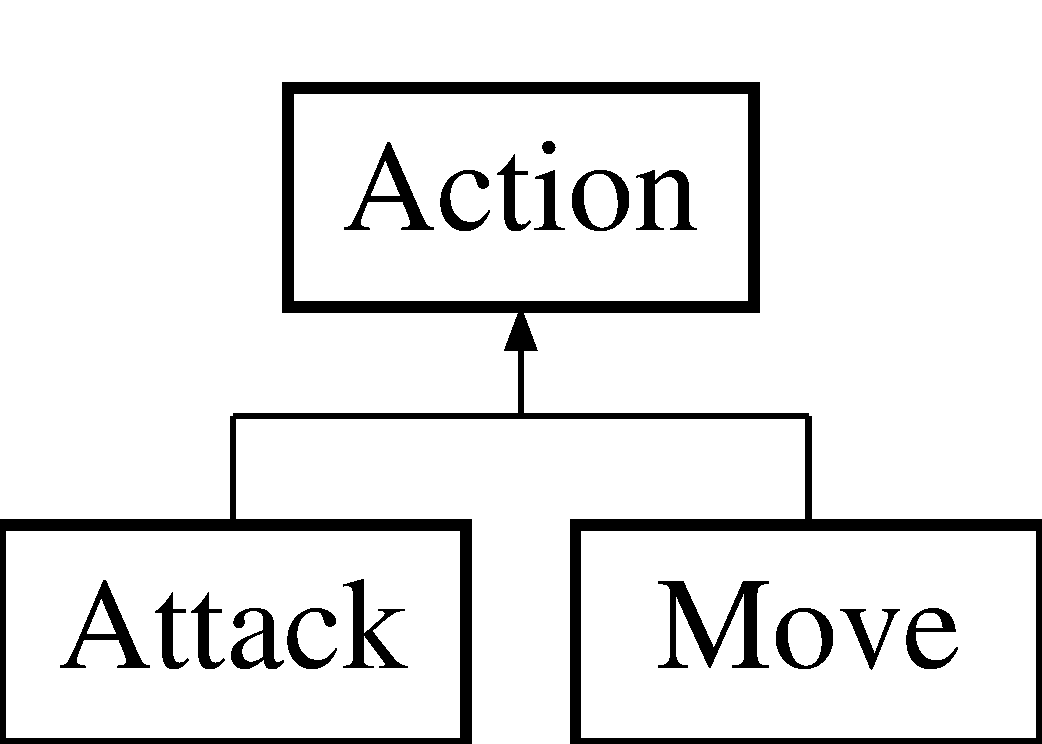
\includegraphics[height=2.000000cm]{class_action}
\end{center}
\end{figure}
\subsection*{Public Member Functions}
\begin{DoxyCompactItemize}
\item 
\hyperlink{class_action_a97da8add4b456b38347ad3447e136d48}{Action} (\hyperlink{class_actor}{Actor} $\ast$\-\_\-actor, std\-::string \&dirname)
\item 
\hyperlink{class_actor}{Actor} $\ast$ \hyperlink{class_action_a7dd87350cb42eccbf2d096eb4f1f9a85}{get\-\_\-actor} ()
\item 
\hyperlink{class_direction}{Direction} \hyperlink{class_action_a26fff2d0b1eaf0109170fe6d8fe77879}{get\-\_\-dir} ()
\item 
virtual bool \hyperlink{class_action_a18a2520db7750f26d7a571c990b82daf}{execute} (\hyperlink{class_game}{Game} $\ast$g)=0
\end{DoxyCompactItemize}
\subsection*{Protected Attributes}
\begin{DoxyCompactItemize}
\item 
\hyperlink{class_actor}{Actor} $\ast$ \hyperlink{class_action_aead5ee9e455a9b0033aca036776c255b}{actor}
\item 
\hyperlink{class_direction}{Direction} \hyperlink{class_action_a04c069c93bbaf099b040379ed976c936}{dir}
\end{DoxyCompactItemize}


\subsection{Constructor \& Destructor Documentation}
\hypertarget{class_action_a97da8add4b456b38347ad3447e136d48}{\index{Action@{Action}!Action@{Action}}
\index{Action@{Action}!Action@{Action}}
\subsubsection[{Action}]{\setlength{\rightskip}{0pt plus 5cm}Action\-::\-Action (
\begin{DoxyParamCaption}
\item[{{\bf Actor} $\ast$}]{\-\_\-actor, }
\item[{std\-::string \&}]{dirname}
\end{DoxyParamCaption}
)}}\label{class_action_a97da8add4b456b38347ad3447e136d48}


\subsection{Member Function Documentation}
\hypertarget{class_action_a18a2520db7750f26d7a571c990b82daf}{\index{Action@{Action}!execute@{execute}}
\index{execute@{execute}!Action@{Action}}
\subsubsection[{execute}]{\setlength{\rightskip}{0pt plus 5cm}virtual bool Action\-::execute (
\begin{DoxyParamCaption}
\item[{{\bf Game} $\ast$}]{g}
\end{DoxyParamCaption}
)\hspace{0.3cm}{\ttfamily [pure virtual]}}}\label{class_action_a18a2520db7750f26d7a571c990b82daf}


Implemented in \hyperlink{class_attack_a8d75db51289fb19f9e9d3d119426e008}{Attack}, and \hyperlink{class_move_a3fbaa547d4a9f9311a326d584c6c0de5}{Move}.

\hypertarget{class_action_a7dd87350cb42eccbf2d096eb4f1f9a85}{\index{Action@{Action}!get\-\_\-actor@{get\-\_\-actor}}
\index{get\-\_\-actor@{get\-\_\-actor}!Action@{Action}}
\subsubsection[{get\-\_\-actor}]{\setlength{\rightskip}{0pt plus 5cm}{\bf Actor} $\ast$ Action\-::get\-\_\-actor (
\begin{DoxyParamCaption}
{}
\end{DoxyParamCaption}
)}}\label{class_action_a7dd87350cb42eccbf2d096eb4f1f9a85}
\hypertarget{class_action_a26fff2d0b1eaf0109170fe6d8fe77879}{\index{Action@{Action}!get\-\_\-dir@{get\-\_\-dir}}
\index{get\-\_\-dir@{get\-\_\-dir}!Action@{Action}}
\subsubsection[{get\-\_\-dir}]{\setlength{\rightskip}{0pt plus 5cm}{\bf Direction} Action\-::get\-\_\-dir (
\begin{DoxyParamCaption}
{}
\end{DoxyParamCaption}
)}}\label{class_action_a26fff2d0b1eaf0109170fe6d8fe77879}


\subsection{Member Data Documentation}
\hypertarget{class_action_aead5ee9e455a9b0033aca036776c255b}{\index{Action@{Action}!actor@{actor}}
\index{actor@{actor}!Action@{Action}}
\subsubsection[{actor}]{\setlength{\rightskip}{0pt plus 5cm}{\bf Actor}$\ast$ Action\-::actor\hspace{0.3cm}{\ttfamily [protected]}}}\label{class_action_aead5ee9e455a9b0033aca036776c255b}
\hypertarget{class_action_a04c069c93bbaf099b040379ed976c936}{\index{Action@{Action}!dir@{dir}}
\index{dir@{dir}!Action@{Action}}
\subsubsection[{dir}]{\setlength{\rightskip}{0pt plus 5cm}{\bf Direction} Action\-::dir\hspace{0.3cm}{\ttfamily [protected]}}}\label{class_action_a04c069c93bbaf099b040379ed976c936}


The documentation for this class was generated from the following files\-:\begin{DoxyCompactItemize}
\item 
actions/\hyperlink{actions_8h}{actions.\-h}\item 
actions/\hyperlink{actions_8cpp}{actions.\-cpp}\end{DoxyCompactItemize}

\hypertarget{class_action__parser}{\section{Action\-\_\-parser Class Reference}
\label{class_action__parser}\index{Action\-\_\-parser@{Action\-\_\-parser}}
}


{\ttfamily \#include $<$action\-\_\-parser.\-h$>$}

Inheritance diagram for Action\-\_\-parser\-:\begin{figure}[H]
\begin{center}
\leavevmode
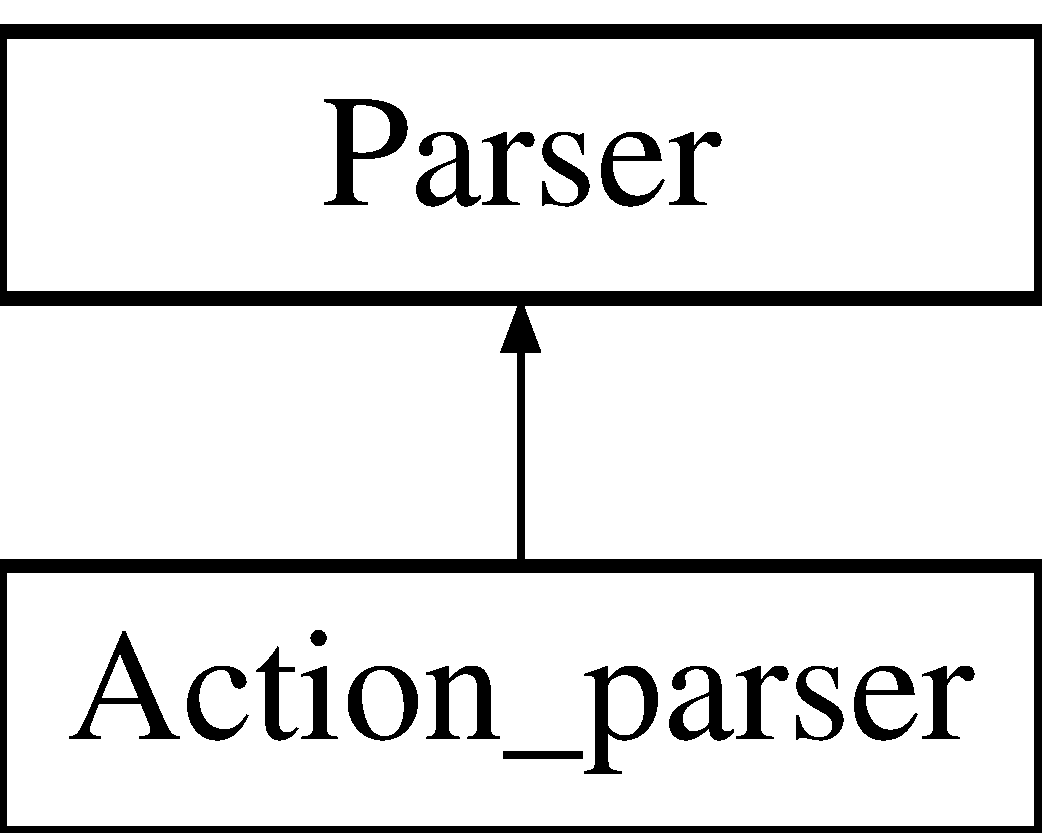
\includegraphics[height=2.000000cm]{class_action__parser}
\end{center}
\end{figure}
\subsection*{Public Member Functions}
\begin{DoxyCompactItemize}
\item 
\hyperlink{class_action__parser_a3c55a5dc1dacc4679fd8cf805a13845d}{Action\-\_\-parser} (std\-::ostream $\ast$stream, std\-::string filename)
\item 
\hyperlink{class_action__parser_a7fa6713374665d4f749a6fd512a45c80}{Action\-\_\-parser} ()=default
\item 
std\-::list$<$ \hyperlink{class_action}{Action} $\ast$ $>$ \hyperlink{class_action__parser_ac7663555d2b2d60dd764304a23f7b164}{parse\-\_\-action} (Ti\-Xml\-Element $\ast$move\-\_\-elem, \hyperlink{class_game}{Game} $\ast$g)
\end{DoxyCompactItemize}
\subsection*{Additional Inherited Members}


\subsection{Constructor \& Destructor Documentation}
\hypertarget{class_action__parser_a3c55a5dc1dacc4679fd8cf805a13845d}{\index{Action\-\_\-parser@{Action\-\_\-parser}!Action\-\_\-parser@{Action\-\_\-parser}}
\index{Action\-\_\-parser@{Action\-\_\-parser}!Action_parser@{Action\-\_\-parser}}
\subsubsection[{Action\-\_\-parser}]{\setlength{\rightskip}{0pt plus 5cm}Action\-\_\-parser\-::\-Action\-\_\-parser (
\begin{DoxyParamCaption}
\item[{std\-::ostream $\ast$}]{stream, }
\item[{std\-::string}]{filename}
\end{DoxyParamCaption}
)}}\label{class_action__parser_a3c55a5dc1dacc4679fd8cf805a13845d}
\hypertarget{class_action__parser_a7fa6713374665d4f749a6fd512a45c80}{\index{Action\-\_\-parser@{Action\-\_\-parser}!Action\-\_\-parser@{Action\-\_\-parser}}
\index{Action\-\_\-parser@{Action\-\_\-parser}!Action_parser@{Action\-\_\-parser}}
\subsubsection[{Action\-\_\-parser}]{\setlength{\rightskip}{0pt plus 5cm}Action\-\_\-parser\-::\-Action\-\_\-parser (
\begin{DoxyParamCaption}
{}
\end{DoxyParamCaption}
)\hspace{0.3cm}{\ttfamily [default]}}}\label{class_action__parser_a7fa6713374665d4f749a6fd512a45c80}


\subsection{Member Function Documentation}
\hypertarget{class_action__parser_ac7663555d2b2d60dd764304a23f7b164}{\index{Action\-\_\-parser@{Action\-\_\-parser}!parse\-\_\-action@{parse\-\_\-action}}
\index{parse\-\_\-action@{parse\-\_\-action}!Action_parser@{Action\-\_\-parser}}
\subsubsection[{parse\-\_\-action}]{\setlength{\rightskip}{0pt plus 5cm}std\-::list$<$ {\bf Action} $\ast$ $>$ Action\-\_\-parser\-::parse\-\_\-action (
\begin{DoxyParamCaption}
\item[{Ti\-Xml\-Element $\ast$}]{move\-\_\-elem, }
\item[{{\bf Game} $\ast$}]{g}
\end{DoxyParamCaption}
)}}\label{class_action__parser_ac7663555d2b2d60dd764304a23f7b164}


The documentation for this class was generated from the following files\-:\begin{DoxyCompactItemize}
\item 
parsers/\hyperlink{action__parser_8h}{action\-\_\-parser.\-h}\item 
parsers/\hyperlink{action__parser_8cpp}{action\-\_\-parser.\-cpp}\end{DoxyCompactItemize}

\hypertarget{class_actor}{\section{Actor Class Reference}
\label{class_actor}\index{Actor@{Actor}}
}


{\ttfamily \#include $<$actor.\-h$>$}

Inheritance diagram for Actor\-:\begin{figure}[H]
\begin{center}
\leavevmode
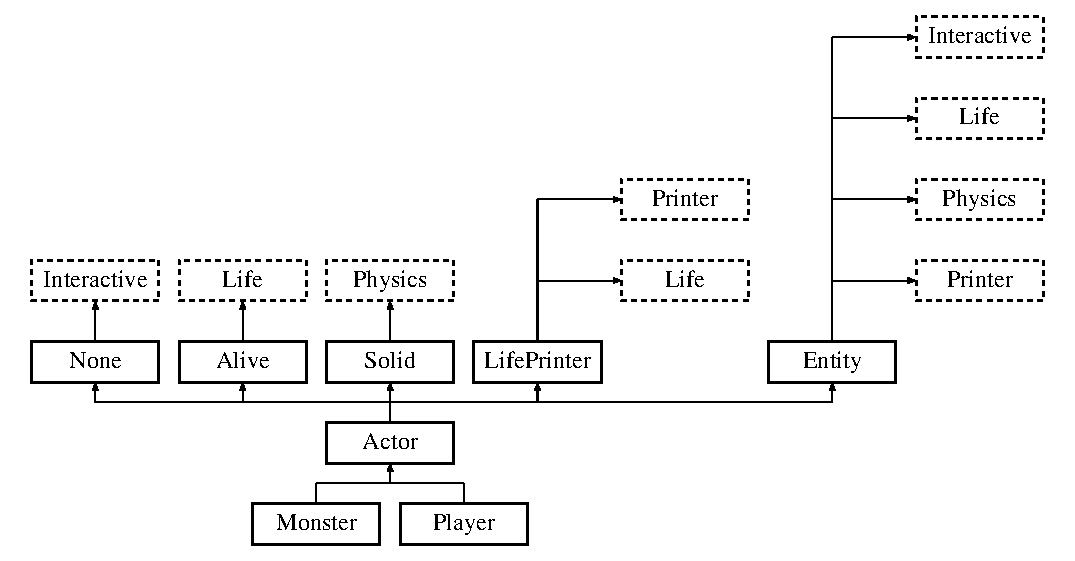
\includegraphics[height=7.000000cm]{class_actor}
\end{center}
\end{figure}
\subsection*{Public Member Functions}
\begin{DoxyCompactItemize}
\item 
\hyperlink{class_actor_a4589af12f18a05c3c9bc69624b2c4eaf}{Actor} (unsigned int \hyperlink{class_entity_afa8f48eccdb09a290e2c1ded3f135363}{x}, unsigned \hyperlink{class_entity_a9d39843430829a89bb8233dbaadae4f1}{y}, char print, std\-::string \-\_\-name)
\item 
std\-::string \& \hyperlink{class_actor_a3f29c558595d47ad9620a78bb5e21f1a}{get\-\_\-name} ()
\end{DoxyCompactItemize}
\subsection*{Additional Inherited Members}


\subsection{Constructor \& Destructor Documentation}
\hypertarget{class_actor_a4589af12f18a05c3c9bc69624b2c4eaf}{\index{Actor@{Actor}!Actor@{Actor}}
\index{Actor@{Actor}!Actor@{Actor}}
\subsubsection[{Actor}]{\setlength{\rightskip}{0pt plus 5cm}Actor\-::\-Actor (
\begin{DoxyParamCaption}
\item[{unsigned int}]{x, }
\item[{unsigned}]{y, }
\item[{char}]{print, }
\item[{std\-::string}]{\-\_\-name}
\end{DoxyParamCaption}
)}}\label{class_actor_a4589af12f18a05c3c9bc69624b2c4eaf}
E\-N\-S\-U\-R\-E(\hyperlink{class_entity_af7f20142aa7883ca29a91c43e3511e48}{properly\-Initialized()}, \char`\"{}\-Constructor must end...\char`\"{}) 

\subsection{Member Function Documentation}
\hypertarget{class_actor_a3f29c558595d47ad9620a78bb5e21f1a}{\index{Actor@{Actor}!get\-\_\-name@{get\-\_\-name}}
\index{get\-\_\-name@{get\-\_\-name}!Actor@{Actor}}
\subsubsection[{get\-\_\-name}]{\setlength{\rightskip}{0pt plus 5cm}std\-::string \& Actor\-::get\-\_\-name (
\begin{DoxyParamCaption}
{}
\end{DoxyParamCaption}
)}}\label{class_actor_a3f29c558595d47ad9620a78bb5e21f1a}
R\-E\-Q\-U\-I\-R\-E(\hyperlink{class_entity_af7f20142aa7883ca29a91c43e3511e48}{properly\-Initialized()}, \char`\"{}\-Actor wasn't initialized when calling get\-\_\-name\char`\"{}) 

The documentation for this class was generated from the following files\-:\begin{DoxyCompactItemize}
\item 
entities/\hyperlink{actor_8h}{actor.\-h}\item 
entities/\hyperlink{actor_8cpp}{actor.\-cpp}\end{DoxyCompactItemize}

\hypertarget{class_actor__parser}{\section{Actor\-\_\-parser Class Reference}
\label{class_actor__parser}\index{Actor\-\_\-parser@{Actor\-\_\-parser}}
}


{\ttfamily \#include $<$actor\-\_\-parser.\-h$>$}

Inheritance diagram for Actor\-\_\-parser\-:\begin{figure}[H]
\begin{center}
\leavevmode
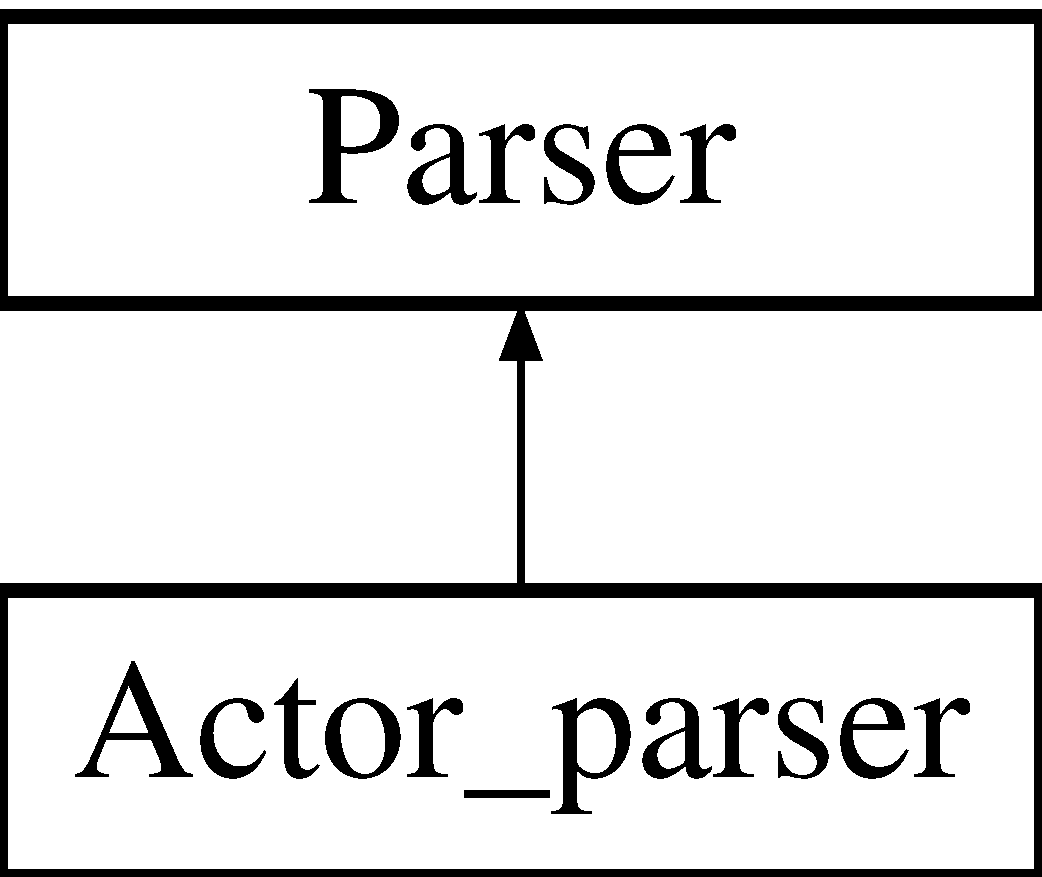
\includegraphics[height=2.000000cm]{class_actor__parser}
\end{center}
\end{figure}
\subsection*{Public Member Functions}
\begin{DoxyCompactItemize}
\item 
\hyperlink{class_actor__parser_ac313d2d8f57b99a7d207c1fe73d6dcdc}{Actor\-\_\-parser} (std\-::ostream $\ast$stream, std\-::string filename)
\item 
\hyperlink{class_actor__parser_a663d1598bbe15d136c86ac198d989eb0}{Actor\-\_\-parser} ()=default
\item 
\hyperlink{class_actor}{Actor} $\ast$ \hyperlink{class_actor__parser_a352d0ccca7a9412a507bd8f304992c98}{parse\-\_\-player} (Ti\-Xml\-Element $\ast$elem, \hyperlink{class_game_a11e553861e3a7fc842680e55171ed06f}{Game\-::\-Playermap} \&\-\_\-players, \hyperlink{class_board}{Board} \&\-\_\-board)
\item 
\hyperlink{class_actor}{Actor} $\ast$ \hyperlink{class_actor__parser_aa8e7ef952116829399ea6fd2f03e47ed}{parse\-\_\-monster} (Ti\-Xml\-Element $\ast$elem, \hyperlink{class_game_a2c39481e575abd66baa206771c504149}{Game\-::\-Monstermap} \&\-\_\-monsters, \hyperlink{class_board}{Board} \&\-\_\-board)
\end{DoxyCompactItemize}
\subsection*{Additional Inherited Members}


\subsection{Constructor \& Destructor Documentation}
\hypertarget{class_actor__parser_ac313d2d8f57b99a7d207c1fe73d6dcdc}{\index{Actor\-\_\-parser@{Actor\-\_\-parser}!Actor\-\_\-parser@{Actor\-\_\-parser}}
\index{Actor\-\_\-parser@{Actor\-\_\-parser}!Actor_parser@{Actor\-\_\-parser}}
\subsubsection[{Actor\-\_\-parser}]{\setlength{\rightskip}{0pt plus 5cm}Actor\-\_\-parser\-::\-Actor\-\_\-parser (
\begin{DoxyParamCaption}
\item[{std\-::ostream $\ast$}]{stream, }
\item[{std\-::string}]{filename}
\end{DoxyParamCaption}
)}}\label{class_actor__parser_ac313d2d8f57b99a7d207c1fe73d6dcdc}
\hypertarget{class_actor__parser_a663d1598bbe15d136c86ac198d989eb0}{\index{Actor\-\_\-parser@{Actor\-\_\-parser}!Actor\-\_\-parser@{Actor\-\_\-parser}}
\index{Actor\-\_\-parser@{Actor\-\_\-parser}!Actor_parser@{Actor\-\_\-parser}}
\subsubsection[{Actor\-\_\-parser}]{\setlength{\rightskip}{0pt plus 5cm}Actor\-\_\-parser\-::\-Actor\-\_\-parser (
\begin{DoxyParamCaption}
{}
\end{DoxyParamCaption}
)\hspace{0.3cm}{\ttfamily [default]}}}\label{class_actor__parser_a663d1598bbe15d136c86ac198d989eb0}


\subsection{Member Function Documentation}
\hypertarget{class_actor__parser_aa8e7ef952116829399ea6fd2f03e47ed}{\index{Actor\-\_\-parser@{Actor\-\_\-parser}!parse\-\_\-monster@{parse\-\_\-monster}}
\index{parse\-\_\-monster@{parse\-\_\-monster}!Actor_parser@{Actor\-\_\-parser}}
\subsubsection[{parse\-\_\-monster}]{\setlength{\rightskip}{0pt plus 5cm}{\bf Actor} $\ast$ Actor\-\_\-parser\-::parse\-\_\-monster (
\begin{DoxyParamCaption}
\item[{Ti\-Xml\-Element $\ast$}]{elem, }
\item[{{\bf Game\-::\-Monstermap} \&}]{\-\_\-monsters, }
\item[{{\bf Board} \&}]{\-\_\-board}
\end{DoxyParamCaption}
)}}\label{class_actor__parser_aa8e7ef952116829399ea6fd2f03e47ed}
\hypertarget{class_actor__parser_a352d0ccca7a9412a507bd8f304992c98}{\index{Actor\-\_\-parser@{Actor\-\_\-parser}!parse\-\_\-player@{parse\-\_\-player}}
\index{parse\-\_\-player@{parse\-\_\-player}!Actor_parser@{Actor\-\_\-parser}}
\subsubsection[{parse\-\_\-player}]{\setlength{\rightskip}{0pt plus 5cm}{\bf Actor} $\ast$ Actor\-\_\-parser\-::parse\-\_\-player (
\begin{DoxyParamCaption}
\item[{Ti\-Xml\-Element $\ast$}]{elem, }
\item[{{\bf Game\-::\-Playermap} \&}]{\-\_\-players, }
\item[{{\bf Board} \&}]{\-\_\-board}
\end{DoxyParamCaption}
)}}\label{class_actor__parser_a352d0ccca7a9412a507bd8f304992c98}


The documentation for this class was generated from the following files\-:\begin{DoxyCompactItemize}
\item 
parsers/\hyperlink{actor__parser_8h}{actor\-\_\-parser.\-h}\item 
parsers/\hyperlink{actor__parser_8cpp}{actor\-\_\-parser.\-cpp}\end{DoxyCompactItemize}

\hypertarget{class_alive}{\section{Alive Class Reference}
\label{class_alive}\index{Alive@{Alive}}
}


{\ttfamily \#include $<$alive.\-h$>$}

Inheritance diagram for Alive\-:\begin{figure}[H]
\begin{center}
\leavevmode
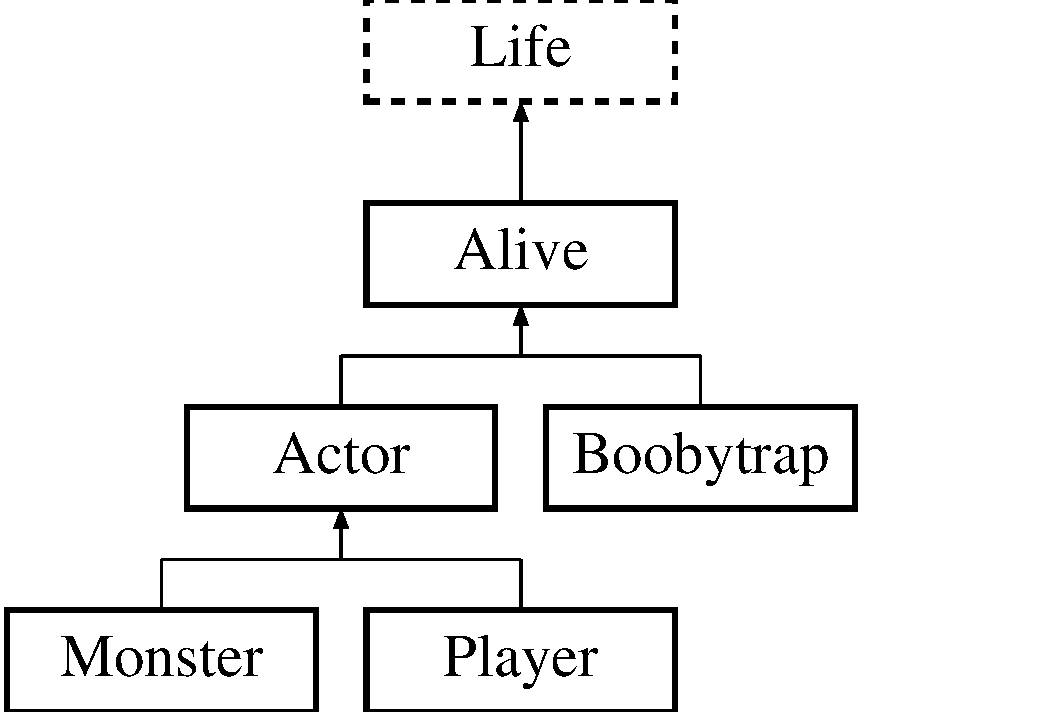
\includegraphics[height=4.000000cm]{class_alive}
\end{center}
\end{figure}
\subsection*{Public Member Functions}
\begin{DoxyCompactItemize}
\item 
\hyperlink{class_alive_ab125282112512443da759822eac32423}{Alive} (int lives)
\item 
bool \hyperlink{class_alive_a35db3016aaa9bbea5e9bcaa4965581b6}{is\-\_\-alive} ()
\item 
void \hyperlink{class_alive_aa10e42533e1f6277ce7da1ca9a2d0b71}{kill} ()
\end{DoxyCompactItemize}


\subsection{Constructor \& Destructor Documentation}
\hypertarget{class_alive_ab125282112512443da759822eac32423}{\index{Alive@{Alive}!Alive@{Alive}}
\index{Alive@{Alive}!Alive@{Alive}}
\subsubsection[{Alive}]{\setlength{\rightskip}{0pt plus 5cm}Alive\-::\-Alive (
\begin{DoxyParamCaption}
\item[{int}]{lives}
\end{DoxyParamCaption}
)}}\label{class_alive_ab125282112512443da759822eac32423}


\subsection{Member Function Documentation}
\hypertarget{class_alive_a35db3016aaa9bbea5e9bcaa4965581b6}{\index{Alive@{Alive}!is\-\_\-alive@{is\-\_\-alive}}
\index{is\-\_\-alive@{is\-\_\-alive}!Alive@{Alive}}
\subsubsection[{is\-\_\-alive}]{\setlength{\rightskip}{0pt plus 5cm}bool Alive\-::is\-\_\-alive (
\begin{DoxyParamCaption}
{}
\end{DoxyParamCaption}
)\hspace{0.3cm}{\ttfamily [virtual]}}}\label{class_alive_a35db3016aaa9bbea5e9bcaa4965581b6}


Implements \hyperlink{class_life_a8f79fb2cb57ef2a76e0c0feba345c68c}{Life}.

\hypertarget{class_alive_aa10e42533e1f6277ce7da1ca9a2d0b71}{\index{Alive@{Alive}!kill@{kill}}
\index{kill@{kill}!Alive@{Alive}}
\subsubsection[{kill}]{\setlength{\rightskip}{0pt plus 5cm}void Alive\-::kill (
\begin{DoxyParamCaption}
{}
\end{DoxyParamCaption}
)\hspace{0.3cm}{\ttfamily [virtual]}}}\label{class_alive_aa10e42533e1f6277ce7da1ca9a2d0b71}


Implements \hyperlink{class_life_a40b24b079b08e3a80a582eff6be8faa3}{Life}.



The documentation for this class was generated from the following files\-:\begin{DoxyCompactItemize}
\item 
entities/life/\hyperlink{alive_8h}{alive.\-h}\item 
entities/life/\hyperlink{alive_8cpp}{alive.\-cpp}\end{DoxyCompactItemize}

\hypertarget{classprecompile_1_1_argument}{\section{precompile.\-Argument Class Reference}
\label{classprecompile_1_1_argument}\index{precompile.\-Argument@{precompile.\-Argument}}
}
\subsection*{Public Member Functions}
\begin{DoxyCompactItemize}
\item 
def \hyperlink{classprecompile_1_1_argument_abce37c1daf9d6821f781dc91c51f5c25}{\-\_\-\-\_\-init\-\_\-\-\_\-}
\item 
def \hyperlink{classprecompile_1_1_argument_ae5b43769fe123f0f8d5621bb9704f404}{define}
\end{DoxyCompactItemize}
\subsection*{Public Attributes}
\begin{DoxyCompactItemize}
\item 
\hyperlink{classprecompile_1_1_argument_a0d0070b1c8143a6a85a467057ccdaa30}{typename}
\item 
\hyperlink{classprecompile_1_1_argument_ac93435d982bf89951e502a0329ec5908}{name}
\end{DoxyCompactItemize}


\subsection{Constructor \& Destructor Documentation}
\hypertarget{classprecompile_1_1_argument_abce37c1daf9d6821f781dc91c51f5c25}{\index{precompile\-::\-Argument@{precompile\-::\-Argument}!\-\_\-\-\_\-init\-\_\-\-\_\-@{\-\_\-\-\_\-init\-\_\-\-\_\-}}
\index{\-\_\-\-\_\-init\-\_\-\-\_\-@{\-\_\-\-\_\-init\-\_\-\-\_\-}!precompile::Argument@{precompile\-::\-Argument}}
\subsubsection[{\-\_\-\-\_\-init\-\_\-\-\_\-}]{\setlength{\rightskip}{0pt plus 5cm}def precompile.\-Argument.\-\_\-\-\_\-init\-\_\-\-\_\- (
\begin{DoxyParamCaption}
\item[{}]{self, }
\item[{}]{typename, }
\item[{}]{name}
\end{DoxyParamCaption}
)}}\label{classprecompile_1_1_argument_abce37c1daf9d6821f781dc91c51f5c25}


\subsection{Member Function Documentation}
\hypertarget{classprecompile_1_1_argument_ae5b43769fe123f0f8d5621bb9704f404}{\index{precompile\-::\-Argument@{precompile\-::\-Argument}!define@{define}}
\index{define@{define}!precompile::Argument@{precompile\-::\-Argument}}
\subsubsection[{define}]{\setlength{\rightskip}{0pt plus 5cm}def precompile.\-Argument.\-define (
\begin{DoxyParamCaption}
\item[{}]{self}
\end{DoxyParamCaption}
)}}\label{classprecompile_1_1_argument_ae5b43769fe123f0f8d5621bb9704f404}


\subsection{Member Data Documentation}
\hypertarget{classprecompile_1_1_argument_ac93435d982bf89951e502a0329ec5908}{\index{precompile\-::\-Argument@{precompile\-::\-Argument}!name@{name}}
\index{name@{name}!precompile::Argument@{precompile\-::\-Argument}}
\subsubsection[{name}]{\setlength{\rightskip}{0pt plus 5cm}precompile.\-Argument.\-name}}\label{classprecompile_1_1_argument_ac93435d982bf89951e502a0329ec5908}
\hypertarget{classprecompile_1_1_argument_a0d0070b1c8143a6a85a467057ccdaa30}{\index{precompile\-::\-Argument@{precompile\-::\-Argument}!typename@{typename}}
\index{typename@{typename}!precompile::Argument@{precompile\-::\-Argument}}
\subsubsection[{typename}]{\setlength{\rightskip}{0pt plus 5cm}precompile.\-Argument.\-typename}}\label{classprecompile_1_1_argument_a0d0070b1c8143a6a85a467057ccdaa30}


The documentation for this class was generated from the following file\-:\begin{DoxyCompactItemize}
\item 
events/dispatch/\hyperlink{precompile_8py}{precompile.\-py}\end{DoxyCompactItemize}

\hypertarget{class_attack}{\section{Attack Class Reference}
\label{class_attack}\index{Attack@{Attack}}
}


{\ttfamily \#include $<$attack.\-h$>$}

Inheritance diagram for Attack\-:\begin{figure}[H]
\begin{center}
\leavevmode
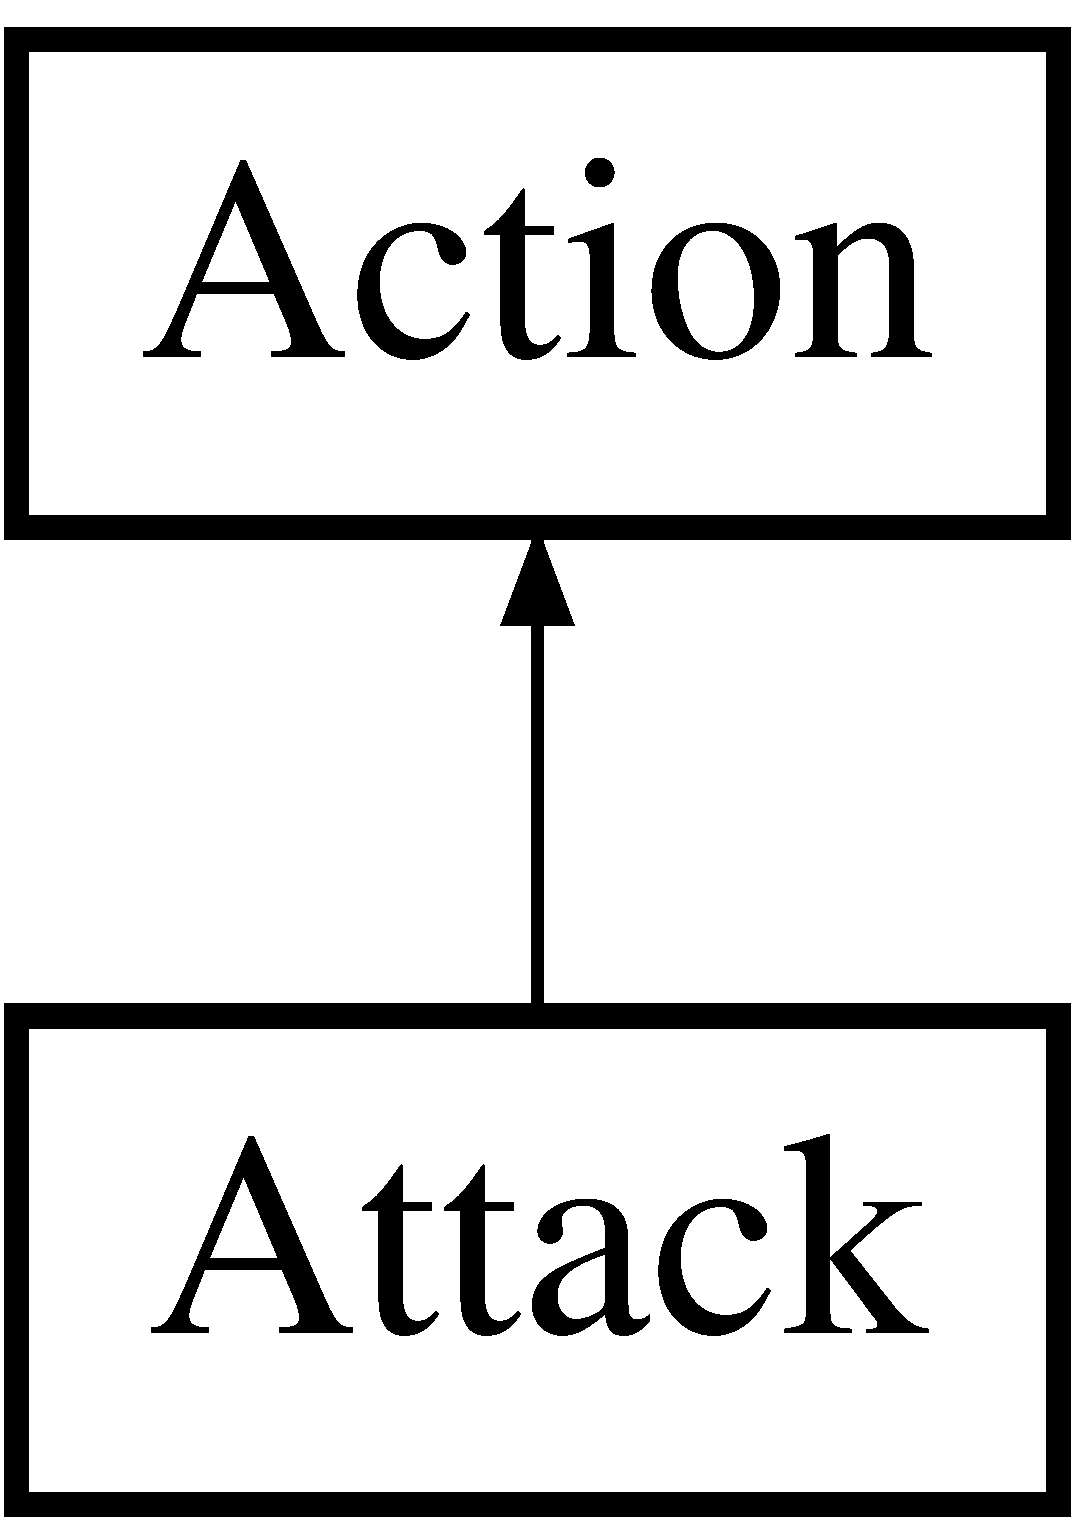
\includegraphics[height=2.000000cm]{class_attack}
\end{center}
\end{figure}
\subsection*{Public Member Functions}
\begin{DoxyCompactItemize}
\item 
\hyperlink{class_attack_ac329e732c451fed73bf14ad2f3731acc}{Attack} (\hyperlink{class_player}{Player} $\ast$player, std\-::string \&dirname)
\item 
bool \hyperlink{class_attack_a8d75db51289fb19f9e9d3d119426e008}{execute} (\hyperlink{class_game}{Game} $\ast$g)
\end{DoxyCompactItemize}
\subsection*{Additional Inherited Members}


\subsection{Constructor \& Destructor Documentation}
\hypertarget{class_attack_ac329e732c451fed73bf14ad2f3731acc}{\index{Attack@{Attack}!Attack@{Attack}}
\index{Attack@{Attack}!Attack@{Attack}}
\subsubsection[{Attack}]{\setlength{\rightskip}{0pt plus 5cm}Attack\-::\-Attack (
\begin{DoxyParamCaption}
\item[{{\bf Player} $\ast$}]{player, }
\item[{std\-::string \&}]{dirname}
\end{DoxyParamCaption}
)}}\label{class_attack_ac329e732c451fed73bf14ad2f3731acc}


\subsection{Member Function Documentation}
\hypertarget{class_attack_a8d75db51289fb19f9e9d3d119426e008}{\index{Attack@{Attack}!execute@{execute}}
\index{execute@{execute}!Attack@{Attack}}
\subsubsection[{execute}]{\setlength{\rightskip}{0pt plus 5cm}bool Attack\-::execute (
\begin{DoxyParamCaption}
\item[{{\bf Game} $\ast$}]{g}
\end{DoxyParamCaption}
)\hspace{0.3cm}{\ttfamily [virtual]}}}\label{class_attack_a8d75db51289fb19f9e9d3d119426e008}


Implements \hyperlink{class_action_a18a2520db7750f26d7a571c990b82daf}{Action}.



The documentation for this class was generated from the following files\-:\begin{DoxyCompactItemize}
\item 
actions/\hyperlink{attack_8h}{attack.\-h}\item 
actions/\hyperlink{attack_8cpp}{attack.\-cpp}\end{DoxyCompactItemize}

\hypertarget{class_barrel}{\section{Barrel Class Reference}
\label{class_barrel}\index{Barrel@{Barrel}}
}


{\ttfamily \#include $<$barrel.\-h$>$}

Inheritance diagram for Barrel\-:\begin{figure}[H]
\begin{center}
\leavevmode
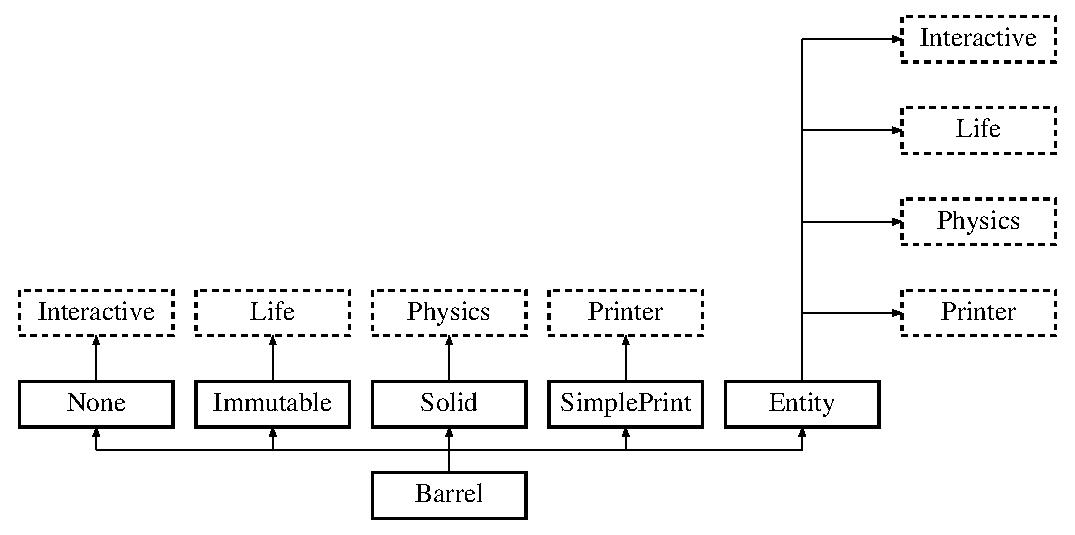
\includegraphics[height=6.000000cm]{class_barrel}
\end{center}
\end{figure}
\subsection*{Public Member Functions}
\begin{DoxyCompactItemize}
\item 
\hyperlink{class_barrel_af0e8147faafe8c847c7250f614055d89}{Barrel} (unsigned int \hyperlink{class_entity_afa8f48eccdb09a290e2c1ded3f135363}{x}, unsigned int \hyperlink{class_entity_a9d39843430829a89bb8233dbaadae4f1}{y})
\item 
void \hyperlink{class_barrel_aebd6e6fda845b455a01d4731286cee67}{info} (std\-::ostream \&out)
\end{DoxyCompactItemize}
\subsection*{Additional Inherited Members}


\subsection{Constructor \& Destructor Documentation}
\hypertarget{class_barrel_af0e8147faafe8c847c7250f614055d89}{\index{Barrel@{Barrel}!Barrel@{Barrel}}
\index{Barrel@{Barrel}!Barrel@{Barrel}}
\subsubsection[{Barrel}]{\setlength{\rightskip}{0pt plus 5cm}Barrel\-::\-Barrel (
\begin{DoxyParamCaption}
\item[{unsigned int}]{x, }
\item[{unsigned int}]{y}
\end{DoxyParamCaption}
)}}\label{class_barrel_af0e8147faafe8c847c7250f614055d89}
E\-N\-S\-U\-R\-E(\hyperlink{class_entity_af7f20142aa7883ca29a91c43e3511e48}{properly\-Initialized()}, \char`\"{}\-Constructor must end...\char`\"{}) 

\subsection{Member Function Documentation}
\hypertarget{class_barrel_aebd6e6fda845b455a01d4731286cee67}{\index{Barrel@{Barrel}!info@{info}}
\index{info@{info}!Barrel@{Barrel}}
\subsubsection[{info}]{\setlength{\rightskip}{0pt plus 5cm}void Barrel\-::info (
\begin{DoxyParamCaption}
\item[{std\-::ostream \&}]{out}
\end{DoxyParamCaption}
)\hspace{0.3cm}{\ttfamily [virtual]}}}\label{class_barrel_aebd6e6fda845b455a01d4731286cee67}
R\-E\-Q\-U\-I\-R\-E(\hyperlink{class_entity_af7f20142aa7883ca29a91c43e3511e48}{properly\-Initialized()}, \char`\"{}\-Barrel wasn't initialized when calling info\char`\"{}) 

Implements \hyperlink{class_entity_aa694874d1f59971187de675d1e0c1fdf}{Entity}.



The documentation for this class was generated from the following files\-:\begin{DoxyCompactItemize}
\item 
entities/\hyperlink{barrel_8h}{barrel.\-h}\item 
entities/\hyperlink{barrel_8cpp}{barrel.\-cpp}\end{DoxyCompactItemize}

\hypertarget{class_board}{\section{Board Class Reference}
\label{class_board}\index{Board@{Board}}
}


{\ttfamily \#include $<$board.\-h$>$}

\subsection*{Public Member Functions}
\begin{DoxyCompactItemize}
\item 
\hyperlink{class_board_a533223f28724623e763587dc401baefa}{Board} (unsigned int \-\_\-width, unsigned int \-\_\-height, \hyperlink{class_game}{Game} $\ast$\-\_\-game)
\item 
\hyperlink{class_entity}{Entity} $\ast$ \hyperlink{class_board_ae58237ab49518bbfec3260152e02335c}{get\-\_\-top} (unsigned int x, unsigned int y)
\item 
void \hyperlink{class_board_a91b01e0fb35aa30fb60252867fedb1e7}{clear\-\_\-top} (unsigned int x, unsigned int y)
\item 
\hyperlink{class_entity}{Entity} $\ast$ \hyperlink{class_board_adad073b1a8011cba63eb8c945da9ba28}{get} (unsigned int loc, unsigned int x, unsigned int y)
\item 
void \hyperlink{class_board_a458cae7e6bb9189f7bf0b3ab1036ea6f}{set\-\_\-name} (std\-::string \-\_\-name)
\item 
bool \hyperlink{class_board_a4ea85ce0aad0d905e3757a3531396178}{valid\-\_\-location} (int x, int y)
\item 
int \hyperlink{class_board_a8ee871cbc57f75299eb95652ab1c3411}{location\-\_\-height} (unsigned int x, unsigned int y)
\item 
\hyperlink{class_entity}{Entity} $\ast$ \hyperlink{class_board_ad77efbd5de132a72a97a9307b111f622}{leave\-\_\-top\-\_\-location} (unsigned int x, unsigned int y)
\item 
bool \hyperlink{class_board_a34efaf5d1af34d910525b20a00d8ff34}{enter\-\_\-top\-\_\-location} (\hyperlink{class_entity}{Entity} $\ast$e, unsigned int x, unsigned int y)
\item 
void \hyperlink{class_board_ae4b3c84812939e557a58e92468a2234b}{enter\-\_\-location} (\hyperlink{class_entity}{Entity} $\ast$e, unsigned int x, unsigned int y)
\item 
char \hyperlink{class_board_ac0253eac886de98047fc70833c4832e0}{to\-\_\-char} (unsigned int x, unsigned int y)
\item 
void \hyperlink{class_board_a272e0648e136707f6a652b84526f351c}{simple\-\_\-graphics} (std\-::ostream \&out)
\item 
void \hyperlink{class_board_ae7e407126c1c113669e645a216fc7848}{write\-\_\-board} (std\-::ostream \&out)
\item 
void \hyperlink{class_board_a85fe9fc0472a4658caada2f9ab585868}{print\-\_\-sideview} (unsigned int x, unsigned int y)
\item 
int \hyperlink{class_board_a5eb8b8fd57b54ee43c189e16a9ee577b}{get\-\_\-width} ()
\item 
int \hyperlink{class_board_a82081634443ee5ad9b00626111caf65a}{get\-\_\-height} ()
\item 
\hyperlink{class_game}{Game} $\ast$ \hyperlink{class_board_a7077136173994866ec146dcefa3dfe64}{get\-\_\-game} ()
\item 
\hyperlink{class_board_af73f45730119a1fd8f6670f53f959e68}{$\sim$\-Board} ()
\end{DoxyCompactItemize}


\subsection{Constructor \& Destructor Documentation}
\hypertarget{class_board_a533223f28724623e763587dc401baefa}{\index{Board@{Board}!Board@{Board}}
\index{Board@{Board}!Board@{Board}}
\subsubsection[{Board}]{\setlength{\rightskip}{0pt plus 5cm}Board\-::\-Board (
\begin{DoxyParamCaption}
\item[{unsigned int}]{\-\_\-width, }
\item[{unsigned int}]{\-\_\-height, }
\item[{{\bf Game} $\ast$}]{\-\_\-game}
\end{DoxyParamCaption}
)}}\label{class_board_a533223f28724623e763587dc401baefa}
\hypertarget{class_board_af73f45730119a1fd8f6670f53f959e68}{\index{Board@{Board}!$\sim$\-Board@{$\sim$\-Board}}
\index{$\sim$\-Board@{$\sim$\-Board}!Board@{Board}}
\subsubsection[{$\sim$\-Board}]{\setlength{\rightskip}{0pt plus 5cm}Board\-::$\sim$\-Board (
\begin{DoxyParamCaption}
{}
\end{DoxyParamCaption}
)}}\label{class_board_af73f45730119a1fd8f6670f53f959e68}


\subsection{Member Function Documentation}
\hypertarget{class_board_a91b01e0fb35aa30fb60252867fedb1e7}{\index{Board@{Board}!clear\-\_\-top@{clear\-\_\-top}}
\index{clear\-\_\-top@{clear\-\_\-top}!Board@{Board}}
\subsubsection[{clear\-\_\-top}]{\setlength{\rightskip}{0pt plus 5cm}void Board\-::clear\-\_\-top (
\begin{DoxyParamCaption}
\item[{unsigned int}]{x, }
\item[{unsigned int}]{y}
\end{DoxyParamCaption}
)}}\label{class_board_a91b01e0fb35aa30fb60252867fedb1e7}
\hypertarget{class_board_ae4b3c84812939e557a58e92468a2234b}{\index{Board@{Board}!enter\-\_\-location@{enter\-\_\-location}}
\index{enter\-\_\-location@{enter\-\_\-location}!Board@{Board}}
\subsubsection[{enter\-\_\-location}]{\setlength{\rightskip}{0pt plus 5cm}void Board\-::enter\-\_\-location (
\begin{DoxyParamCaption}
\item[{{\bf Entity} $\ast$}]{e, }
\item[{unsigned int}]{x, }
\item[{unsigned int}]{y}
\end{DoxyParamCaption}
)}}\label{class_board_ae4b3c84812939e557a58e92468a2234b}
\hypertarget{class_board_a34efaf5d1af34d910525b20a00d8ff34}{\index{Board@{Board}!enter\-\_\-top\-\_\-location@{enter\-\_\-top\-\_\-location}}
\index{enter\-\_\-top\-\_\-location@{enter\-\_\-top\-\_\-location}!Board@{Board}}
\subsubsection[{enter\-\_\-top\-\_\-location}]{\setlength{\rightskip}{0pt plus 5cm}bool Board\-::enter\-\_\-top\-\_\-location (
\begin{DoxyParamCaption}
\item[{{\bf Entity} $\ast$}]{e, }
\item[{unsigned int}]{x, }
\item[{unsigned int}]{y}
\end{DoxyParamCaption}
)}}\label{class_board_a34efaf5d1af34d910525b20a00d8ff34}
\hypertarget{class_board_adad073b1a8011cba63eb8c945da9ba28}{\index{Board@{Board}!get@{get}}
\index{get@{get}!Board@{Board}}
\subsubsection[{get}]{\setlength{\rightskip}{0pt plus 5cm}{\bf Entity} $\ast$ Board\-::get (
\begin{DoxyParamCaption}
\item[{unsigned int}]{loc, }
\item[{unsigned int}]{x, }
\item[{unsigned int}]{y}
\end{DoxyParamCaption}
)}}\label{class_board_adad073b1a8011cba63eb8c945da9ba28}
\hypertarget{class_board_a7077136173994866ec146dcefa3dfe64}{\index{Board@{Board}!get\-\_\-game@{get\-\_\-game}}
\index{get\-\_\-game@{get\-\_\-game}!Board@{Board}}
\subsubsection[{get\-\_\-game}]{\setlength{\rightskip}{0pt plus 5cm}{\bf Game} $\ast$ Board\-::get\-\_\-game (
\begin{DoxyParamCaption}
{}
\end{DoxyParamCaption}
)}}\label{class_board_a7077136173994866ec146dcefa3dfe64}
\hypertarget{class_board_a82081634443ee5ad9b00626111caf65a}{\index{Board@{Board}!get\-\_\-height@{get\-\_\-height}}
\index{get\-\_\-height@{get\-\_\-height}!Board@{Board}}
\subsubsection[{get\-\_\-height}]{\setlength{\rightskip}{0pt plus 5cm}int Board\-::get\-\_\-height (
\begin{DoxyParamCaption}
{}
\end{DoxyParamCaption}
)}}\label{class_board_a82081634443ee5ad9b00626111caf65a}
\hypertarget{class_board_ae58237ab49518bbfec3260152e02335c}{\index{Board@{Board}!get\-\_\-top@{get\-\_\-top}}
\index{get\-\_\-top@{get\-\_\-top}!Board@{Board}}
\subsubsection[{get\-\_\-top}]{\setlength{\rightskip}{0pt plus 5cm}{\bf Entity} $\ast$ Board\-::get\-\_\-top (
\begin{DoxyParamCaption}
\item[{unsigned int}]{x, }
\item[{unsigned int}]{y}
\end{DoxyParamCaption}
)}}\label{class_board_ae58237ab49518bbfec3260152e02335c}
\hypertarget{class_board_a5eb8b8fd57b54ee43c189e16a9ee577b}{\index{Board@{Board}!get\-\_\-width@{get\-\_\-width}}
\index{get\-\_\-width@{get\-\_\-width}!Board@{Board}}
\subsubsection[{get\-\_\-width}]{\setlength{\rightskip}{0pt plus 5cm}int Board\-::get\-\_\-width (
\begin{DoxyParamCaption}
{}
\end{DoxyParamCaption}
)}}\label{class_board_a5eb8b8fd57b54ee43c189e16a9ee577b}
\hypertarget{class_board_ad77efbd5de132a72a97a9307b111f622}{\index{Board@{Board}!leave\-\_\-top\-\_\-location@{leave\-\_\-top\-\_\-location}}
\index{leave\-\_\-top\-\_\-location@{leave\-\_\-top\-\_\-location}!Board@{Board}}
\subsubsection[{leave\-\_\-top\-\_\-location}]{\setlength{\rightskip}{0pt plus 5cm}{\bf Entity} $\ast$ Board\-::leave\-\_\-top\-\_\-location (
\begin{DoxyParamCaption}
\item[{unsigned int}]{x, }
\item[{unsigned int}]{y}
\end{DoxyParamCaption}
)}}\label{class_board_ad77efbd5de132a72a97a9307b111f622}
\hypertarget{class_board_a8ee871cbc57f75299eb95652ab1c3411}{\index{Board@{Board}!location\-\_\-height@{location\-\_\-height}}
\index{location\-\_\-height@{location\-\_\-height}!Board@{Board}}
\subsubsection[{location\-\_\-height}]{\setlength{\rightskip}{0pt plus 5cm}int Board\-::location\-\_\-height (
\begin{DoxyParamCaption}
\item[{unsigned int}]{x, }
\item[{unsigned int}]{y}
\end{DoxyParamCaption}
)}}\label{class_board_a8ee871cbc57f75299eb95652ab1c3411}
\hypertarget{class_board_a85fe9fc0472a4658caada2f9ab585868}{\index{Board@{Board}!print\-\_\-sideview@{print\-\_\-sideview}}
\index{print\-\_\-sideview@{print\-\_\-sideview}!Board@{Board}}
\subsubsection[{print\-\_\-sideview}]{\setlength{\rightskip}{0pt plus 5cm}void Board\-::print\-\_\-sideview (
\begin{DoxyParamCaption}
\item[{unsigned int}]{x, }
\item[{unsigned int}]{y}
\end{DoxyParamCaption}
)}}\label{class_board_a85fe9fc0472a4658caada2f9ab585868}
\hypertarget{class_board_a458cae7e6bb9189f7bf0b3ab1036ea6f}{\index{Board@{Board}!set\-\_\-name@{set\-\_\-name}}
\index{set\-\_\-name@{set\-\_\-name}!Board@{Board}}
\subsubsection[{set\-\_\-name}]{\setlength{\rightskip}{0pt plus 5cm}void Board\-::set\-\_\-name (
\begin{DoxyParamCaption}
\item[{std\-::string}]{\-\_\-name}
\end{DoxyParamCaption}
)}}\label{class_board_a458cae7e6bb9189f7bf0b3ab1036ea6f}
\hypertarget{class_board_a272e0648e136707f6a652b84526f351c}{\index{Board@{Board}!simple\-\_\-graphics@{simple\-\_\-graphics}}
\index{simple\-\_\-graphics@{simple\-\_\-graphics}!Board@{Board}}
\subsubsection[{simple\-\_\-graphics}]{\setlength{\rightskip}{0pt plus 5cm}void Board\-::simple\-\_\-graphics (
\begin{DoxyParamCaption}
\item[{std\-::ostream \&}]{out}
\end{DoxyParamCaption}
)}}\label{class_board_a272e0648e136707f6a652b84526f351c}
\hypertarget{class_board_ac0253eac886de98047fc70833c4832e0}{\index{Board@{Board}!to\-\_\-char@{to\-\_\-char}}
\index{to\-\_\-char@{to\-\_\-char}!Board@{Board}}
\subsubsection[{to\-\_\-char}]{\setlength{\rightskip}{0pt plus 5cm}char Board\-::to\-\_\-char (
\begin{DoxyParamCaption}
\item[{unsigned int}]{x, }
\item[{unsigned int}]{y}
\end{DoxyParamCaption}
)}}\label{class_board_ac0253eac886de98047fc70833c4832e0}
\hypertarget{class_board_a4ea85ce0aad0d905e3757a3531396178}{\index{Board@{Board}!valid\-\_\-location@{valid\-\_\-location}}
\index{valid\-\_\-location@{valid\-\_\-location}!Board@{Board}}
\subsubsection[{valid\-\_\-location}]{\setlength{\rightskip}{0pt plus 5cm}bool Board\-::valid\-\_\-location (
\begin{DoxyParamCaption}
\item[{int}]{x, }
\item[{int}]{y}
\end{DoxyParamCaption}
)}}\label{class_board_a4ea85ce0aad0d905e3757a3531396178}
\hypertarget{class_board_ae7e407126c1c113669e645a216fc7848}{\index{Board@{Board}!write\-\_\-board@{write\-\_\-board}}
\index{write\-\_\-board@{write\-\_\-board}!Board@{Board}}
\subsubsection[{write\-\_\-board}]{\setlength{\rightskip}{0pt plus 5cm}void Board\-::write\-\_\-board (
\begin{DoxyParamCaption}
\item[{std\-::ostream \&}]{out}
\end{DoxyParamCaption}
)}}\label{class_board_ae7e407126c1c113669e645a216fc7848}


The documentation for this class was generated from the following files\-:\begin{DoxyCompactItemize}
\item 
game/\hyperlink{board_8h}{board.\-h}\item 
game/\hyperlink{board_8cpp}{board.\-cpp}\end{DoxyCompactItemize}

\hypertarget{classconvert_1_1_board}{\section{convert.\-Board Class Reference}
\label{classconvert_1_1_board}\index{convert.\-Board@{convert.\-Board}}
}
\subsection*{Public Member Functions}
\begin{DoxyCompactItemize}
\item 
def \hyperlink{classconvert_1_1_board_ac83785a587ae14b70b6bbbb03b99f81c}{\-\_\-\-\_\-init\-\_\-\-\_\-}
\item 
def \hyperlink{classconvert_1_1_board_a77e51b0eff8620e0e38ab4e95c050aeb}{newtree}
\end{DoxyCompactItemize}
\subsection*{Public Attributes}
\begin{DoxyCompactItemize}
\item 
\hyperlink{classconvert_1_1_board_ab21be02b600dd26b79e21b3288f4ccff}{naam}
\item 
\hyperlink{classconvert_1_1_board_a36f114a23926efd5dcb472db47615b59}{lengte}
\item 
\hyperlink{classconvert_1_1_board_a06be1a7bc2e6511c3d5ebb8b6e0fccc4}{breedte}
\item 
\hyperlink{classconvert_1_1_board_ace8a4757fdababb59f63d112a309b1ad}{stuff}
\end{DoxyCompactItemize}


\subsection{Constructor \& Destructor Documentation}
\hypertarget{classconvert_1_1_board_ac83785a587ae14b70b6bbbb03b99f81c}{\index{convert\-::\-Board@{convert\-::\-Board}!\-\_\-\-\_\-init\-\_\-\-\_\-@{\-\_\-\-\_\-init\-\_\-\-\_\-}}
\index{\-\_\-\-\_\-init\-\_\-\-\_\-@{\-\_\-\-\_\-init\-\_\-\-\_\-}!convert::Board@{convert\-::\-Board}}
\subsubsection[{\-\_\-\-\_\-init\-\_\-\-\_\-}]{\setlength{\rightskip}{0pt plus 5cm}def convert.\-Board.\-\_\-\-\_\-init\-\_\-\-\_\- (
\begin{DoxyParamCaption}
\item[{}]{self, }
\item[{}]{tree}
\end{DoxyParamCaption}
)}}\label{classconvert_1_1_board_ac83785a587ae14b70b6bbbb03b99f81c}


\subsection{Member Function Documentation}
\hypertarget{classconvert_1_1_board_a77e51b0eff8620e0e38ab4e95c050aeb}{\index{convert\-::\-Board@{convert\-::\-Board}!newtree@{newtree}}
\index{newtree@{newtree}!convert::Board@{convert\-::\-Board}}
\subsubsection[{newtree}]{\setlength{\rightskip}{0pt plus 5cm}def convert.\-Board.\-newtree (
\begin{DoxyParamCaption}
\item[{}]{self}
\end{DoxyParamCaption}
)}}\label{classconvert_1_1_board_a77e51b0eff8620e0e38ab4e95c050aeb}


\subsection{Member Data Documentation}
\hypertarget{classconvert_1_1_board_a06be1a7bc2e6511c3d5ebb8b6e0fccc4}{\index{convert\-::\-Board@{convert\-::\-Board}!breedte@{breedte}}
\index{breedte@{breedte}!convert::Board@{convert\-::\-Board}}
\subsubsection[{breedte}]{\setlength{\rightskip}{0pt plus 5cm}convert.\-Board.\-breedte}}\label{classconvert_1_1_board_a06be1a7bc2e6511c3d5ebb8b6e0fccc4}
\hypertarget{classconvert_1_1_board_a36f114a23926efd5dcb472db47615b59}{\index{convert\-::\-Board@{convert\-::\-Board}!lengte@{lengte}}
\index{lengte@{lengte}!convert::Board@{convert\-::\-Board}}
\subsubsection[{lengte}]{\setlength{\rightskip}{0pt plus 5cm}convert.\-Board.\-lengte}}\label{classconvert_1_1_board_a36f114a23926efd5dcb472db47615b59}
\hypertarget{classconvert_1_1_board_ab21be02b600dd26b79e21b3288f4ccff}{\index{convert\-::\-Board@{convert\-::\-Board}!naam@{naam}}
\index{naam@{naam}!convert::Board@{convert\-::\-Board}}
\subsubsection[{naam}]{\setlength{\rightskip}{0pt plus 5cm}convert.\-Board.\-naam}}\label{classconvert_1_1_board_ab21be02b600dd26b79e21b3288f4ccff}
\hypertarget{classconvert_1_1_board_ace8a4757fdababb59f63d112a309b1ad}{\index{convert\-::\-Board@{convert\-::\-Board}!stuff@{stuff}}
\index{stuff@{stuff}!convert::Board@{convert\-::\-Board}}
\subsubsection[{stuff}]{\setlength{\rightskip}{0pt plus 5cm}convert.\-Board.\-stuff}}\label{classconvert_1_1_board_ace8a4757fdababb59f63d112a309b1ad}


The documentation for this class was generated from the following file\-:\begin{DoxyCompactItemize}
\item 
tests/filetests\-\_\-old/\hyperlink{convert_8py}{convert.\-py}\end{DoxyCompactItemize}

\hypertarget{class_board__parser}{\section{Board\-\_\-parser Class Reference}
\label{class_board__parser}\index{Board\-\_\-parser@{Board\-\_\-parser}}
}


{\ttfamily \#include $<$board\-\_\-parser.\-h$>$}

Inheritance diagram for Board\-\_\-parser\-:\begin{figure}[H]
\begin{center}
\leavevmode
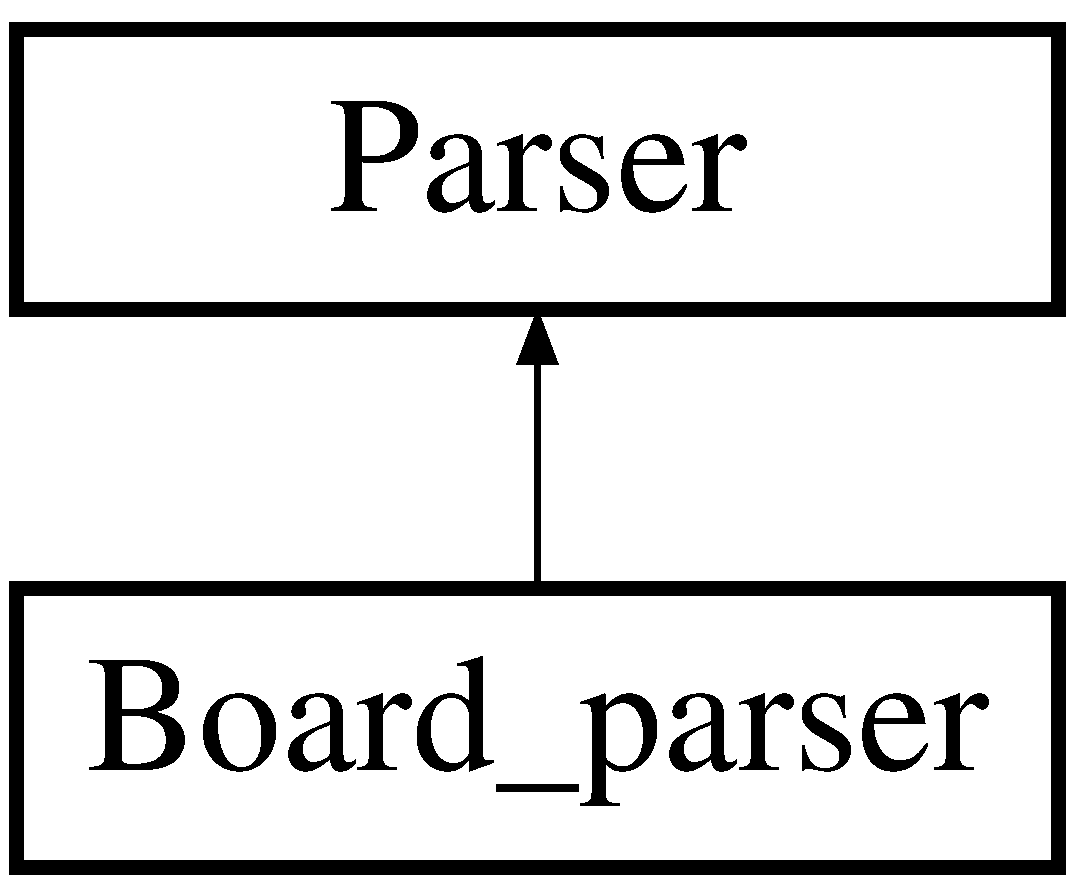
\includegraphics[height=2.000000cm]{class_board__parser}
\end{center}
\end{figure}
\subsection*{Public Member Functions}
\begin{DoxyCompactItemize}
\item 
\hyperlink{class_board__parser_ac319ba5a336e36cfa2415119d879a9d2}{Board\-\_\-parser} (std\-::ostream $\ast$stream, std\-::string filename)
\item 
\hyperlink{class_board__parser_a99271ae26b210b3624c67aeab38033ae}{Board\-\_\-parser} ()=default
\item 
\hyperlink{class_board}{Board} $\ast$ \hyperlink{class_board__parser_a31ec31613ebf8aedb0c8b7fc01c58ffa}{parse\-\_\-board} (Ti\-Xml\-Element $\ast$board\-\_\-elem, \hyperlink{class_game_a11e553861e3a7fc842680e55171ed06f}{Game\-::\-Playermap} \&\-\_\-players, \hyperlink{class_game_a3ac788aaa1e70509a9b9745acd17a8b5}{Game\-::\-Gatemap} \&\-\_\-gates, \hyperlink{class_game_a2c39481e575abd66baa206771c504149}{Game\-::\-Monstermap} \&\-\_\-monsters, \hyperlink{class_game}{Game} $\ast$game)
\end{DoxyCompactItemize}
\subsection*{Additional Inherited Members}


\subsection{Constructor \& Destructor Documentation}
\hypertarget{class_board__parser_ac319ba5a336e36cfa2415119d879a9d2}{\index{Board\-\_\-parser@{Board\-\_\-parser}!Board\-\_\-parser@{Board\-\_\-parser}}
\index{Board\-\_\-parser@{Board\-\_\-parser}!Board_parser@{Board\-\_\-parser}}
\subsubsection[{Board\-\_\-parser}]{\setlength{\rightskip}{0pt plus 5cm}Board\-\_\-parser\-::\-Board\-\_\-parser (
\begin{DoxyParamCaption}
\item[{std\-::ostream $\ast$}]{stream, }
\item[{std\-::string}]{filename}
\end{DoxyParamCaption}
)}}\label{class_board__parser_ac319ba5a336e36cfa2415119d879a9d2}
\hypertarget{class_board__parser_a99271ae26b210b3624c67aeab38033ae}{\index{Board\-\_\-parser@{Board\-\_\-parser}!Board\-\_\-parser@{Board\-\_\-parser}}
\index{Board\-\_\-parser@{Board\-\_\-parser}!Board_parser@{Board\-\_\-parser}}
\subsubsection[{Board\-\_\-parser}]{\setlength{\rightskip}{0pt plus 5cm}Board\-\_\-parser\-::\-Board\-\_\-parser (
\begin{DoxyParamCaption}
{}
\end{DoxyParamCaption}
)\hspace{0.3cm}{\ttfamily [default]}}}\label{class_board__parser_a99271ae26b210b3624c67aeab38033ae}


\subsection{Member Function Documentation}
\hypertarget{class_board__parser_a31ec31613ebf8aedb0c8b7fc01c58ffa}{\index{Board\-\_\-parser@{Board\-\_\-parser}!parse\-\_\-board@{parse\-\_\-board}}
\index{parse\-\_\-board@{parse\-\_\-board}!Board_parser@{Board\-\_\-parser}}
\subsubsection[{parse\-\_\-board}]{\setlength{\rightskip}{0pt plus 5cm}{\bf Board} $\ast$ Board\-\_\-parser\-::parse\-\_\-board (
\begin{DoxyParamCaption}
\item[{Ti\-Xml\-Element $\ast$}]{board\-\_\-elem, }
\item[{{\bf Game\-::\-Playermap} \&}]{\-\_\-players, }
\item[{{\bf Game\-::\-Gatemap} \&}]{\-\_\-gates, }
\item[{{\bf Game\-::\-Monstermap} \&}]{\-\_\-monsters, }
\item[{{\bf Game} $\ast$}]{game}
\end{DoxyParamCaption}
)}}\label{class_board__parser_a31ec31613ebf8aedb0c8b7fc01c58ffa}


The documentation for this class was generated from the following files\-:\begin{DoxyCompactItemize}
\item 
parsers/\hyperlink{board__parser_8h}{board\-\_\-parser.\-h}\item 
parsers/\hyperlink{board__parser_8cpp}{board\-\_\-parser.\-cpp}\end{DoxyCompactItemize}

\hypertarget{class_boobytrap}{\section{Boobytrap Class Reference}
\label{class_boobytrap}\index{Boobytrap@{Boobytrap}}
}


{\ttfamily \#include $<$boobytrap.\-h$>$}

Inheritance diagram for Boobytrap\-:\begin{figure}[H]
\begin{center}
\leavevmode
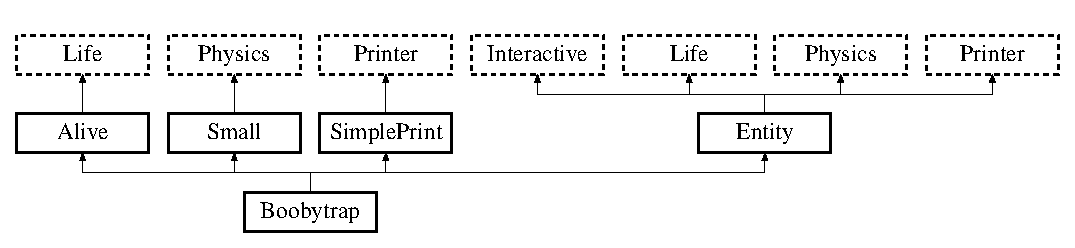
\includegraphics[height=2.891566cm]{class_boobytrap}
\end{center}
\end{figure}
\subsection*{Public Member Functions}
\begin{DoxyCompactItemize}
\item 
\hyperlink{class_boobytrap_af04c92c1eb8cd214ea8c323db5a1a3c9}{Boobytrap} (unsigned int \hyperlink{class_entity_afa8f48eccdb09a290e2c1ded3f135363}{x}, unsigned \hyperlink{class_entity_a9d39843430829a89bb8233dbaadae4f1}{y})
\item 
void \hyperlink{class_boobytrap_aa73f3cbd8027a4ae55e082a62971ef72}{info} (std\-::ostream \&)
\end{DoxyCompactItemize}
\subsection*{Additional Inherited Members}


\subsection{Constructor \& Destructor Documentation}
\hypertarget{class_boobytrap_af04c92c1eb8cd214ea8c323db5a1a3c9}{\index{Boobytrap@{Boobytrap}!Boobytrap@{Boobytrap}}
\index{Boobytrap@{Boobytrap}!Boobytrap@{Boobytrap}}
\subsubsection[{Boobytrap}]{\setlength{\rightskip}{0pt plus 5cm}Boobytrap\-::\-Boobytrap (
\begin{DoxyParamCaption}
\item[{unsigned int}]{x, }
\item[{unsigned}]{y}
\end{DoxyParamCaption}
)}}\label{class_boobytrap_af04c92c1eb8cd214ea8c323db5a1a3c9}
E\-N\-S\-U\-R\-E(\hyperlink{class_entity_af7f20142aa7883ca29a91c43e3511e48}{properly\-Initialized()}, \char`\"{}\-Constructor must end...\char`\"{}) 

\subsection{Member Function Documentation}
\hypertarget{class_boobytrap_aa73f3cbd8027a4ae55e082a62971ef72}{\index{Boobytrap@{Boobytrap}!info@{info}}
\index{info@{info}!Boobytrap@{Boobytrap}}
\subsubsection[{info}]{\setlength{\rightskip}{0pt plus 5cm}void Boobytrap\-::info (
\begin{DoxyParamCaption}
\item[{std\-::ostream \&}]{out}
\end{DoxyParamCaption}
)\hspace{0.3cm}{\ttfamily [virtual]}}}\label{class_boobytrap_aa73f3cbd8027a4ae55e082a62971ef72}
R\-E\-Q\-U\-I\-R\-E(\hyperlink{class_entity_af7f20142aa7883ca29a91c43e3511e48}{properly\-Initialized()}, \char`\"{}\-Boobytrap wasn't initialized when calling info\char`\"{}) 

Implements \hyperlink{class_entity_aa694874d1f59971187de675d1e0c1fdf}{Entity}.



The documentation for this class was generated from the following files\-:\begin{DoxyCompactItemize}
\item 
entities/\hyperlink{boobytrap_8h}{boobytrap.\-h}\item 
entities/\hyperlink{boobytrap_8cpp}{boobytrap.\-cpp}\end{DoxyCompactItemize}

\hypertarget{class_button}{\section{Button Class Reference}
\label{class_button}\index{Button@{Button}}
}


{\ttfamily \#include $<$button.\-h$>$}

Inheritance diagram for Button\-:\begin{figure}[H]
\begin{center}
\leavevmode
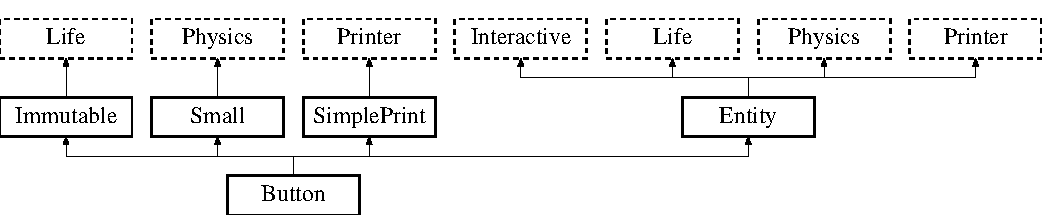
\includegraphics[height=2.891566cm]{class_button}
\end{center}
\end{figure}
\subsection*{Public Member Functions}
\begin{DoxyCompactItemize}
\item 
\hyperlink{class_button_ad6d31876c1b6fd811ed94e52a97e806c}{Button} (unsigned int \hyperlink{class_entity_afa8f48eccdb09a290e2c1ded3f135363}{x}, unsigned \hyperlink{class_entity_a9d39843430829a89bb8233dbaadae4f1}{y}, \hyperlink{class_gate}{Gate} $\ast$\-\_\-gate)
\item 
void \hyperlink{class_button_aba3d89d8caf373ced3f69f24ad09682a}{info} (std\-::ostream \&out)
\end{DoxyCompactItemize}
\subsection*{Friends}
\begin{DoxyCompactItemize}
\item 
class \hyperlink{class_button_ad46435fe6b8e9a384d33d608058862ae}{I\-A\-\_\-\-Enter\-Handler}
\item 
class \hyperlink{class_button_adc4c20007ad2fd4bc2556fbfbff54945}{I\-A\-\_\-\-Leave\-Handler}
\end{DoxyCompactItemize}
\subsection*{Additional Inherited Members}


\subsection{Constructor \& Destructor Documentation}
\hypertarget{class_button_ad6d31876c1b6fd811ed94e52a97e806c}{\index{Button@{Button}!Button@{Button}}
\index{Button@{Button}!Button@{Button}}
\subsubsection[{Button}]{\setlength{\rightskip}{0pt plus 5cm}Button\-::\-Button (
\begin{DoxyParamCaption}
\item[{unsigned int}]{x, }
\item[{unsigned}]{y, }
\item[{{\bf Gate} $\ast$}]{\-\_\-gate}
\end{DoxyParamCaption}
)}}\label{class_button_ad6d31876c1b6fd811ed94e52a97e806c}
E\-N\-S\-U\-R\-E(\hyperlink{class_entity_af7f20142aa7883ca29a91c43e3511e48}{properly\-Initialized()}, \char`\"{}\-Constructor must end...\char`\"{}) 

\subsection{Member Function Documentation}
\hypertarget{class_button_aba3d89d8caf373ced3f69f24ad09682a}{\index{Button@{Button}!info@{info}}
\index{info@{info}!Button@{Button}}
\subsubsection[{info}]{\setlength{\rightskip}{0pt plus 5cm}void Button\-::info (
\begin{DoxyParamCaption}
\item[{std\-::ostream \&}]{out}
\end{DoxyParamCaption}
)\hspace{0.3cm}{\ttfamily [virtual]}}}\label{class_button_aba3d89d8caf373ced3f69f24ad09682a}
R\-E\-Q\-U\-I\-R\-E(\hyperlink{class_entity_af7f20142aa7883ca29a91c43e3511e48}{properly\-Initialized()}, \char`\"{}\-Button wasn't initialized when calling info\char`\"{}) 

Implements \hyperlink{class_entity_aa694874d1f59971187de675d1e0c1fdf}{Entity}.



\subsection{Friends And Related Function Documentation}
\hypertarget{class_button_ad46435fe6b8e9a384d33d608058862ae}{\index{Button@{Button}!I\-A\-\_\-\-Enter\-Handler@{I\-A\-\_\-\-Enter\-Handler}}
\index{I\-A\-\_\-\-Enter\-Handler@{I\-A\-\_\-\-Enter\-Handler}!Button@{Button}}
\subsubsection[{I\-A\-\_\-\-Enter\-Handler}]{\setlength{\rightskip}{0pt plus 5cm}friend class {\bf I\-A\-\_\-\-Enter\-Handler}\hspace{0.3cm}{\ttfamily [friend]}}}\label{class_button_ad46435fe6b8e9a384d33d608058862ae}
\hypertarget{class_button_adc4c20007ad2fd4bc2556fbfbff54945}{\index{Button@{Button}!I\-A\-\_\-\-Leave\-Handler@{I\-A\-\_\-\-Leave\-Handler}}
\index{I\-A\-\_\-\-Leave\-Handler@{I\-A\-\_\-\-Leave\-Handler}!Button@{Button}}
\subsubsection[{I\-A\-\_\-\-Leave\-Handler}]{\setlength{\rightskip}{0pt plus 5cm}friend class {\bf I\-A\-\_\-\-Leave\-Handler}\hspace{0.3cm}{\ttfamily [friend]}}}\label{class_button_adc4c20007ad2fd4bc2556fbfbff54945}


The documentation for this class was generated from the following files\-:\begin{DoxyCompactItemize}
\item 
entities/\hyperlink{button_8h}{button.\-h}\item 
entities/\hyperlink{button_8cpp}{button.\-cpp}\end{DoxyCompactItemize}

\hypertarget{class_collision_dispatch}{\section{Collision\-Dispatch Class Reference}
\label{class_collision_dispatch}\index{Collision\-Dispatch@{Collision\-Dispatch}}
}


{\ttfamily \#include $<$dispatchers.\-h$>$}

Inheritance diagram for Collision\-Dispatch\-:\begin{figure}[H]
\begin{center}
\leavevmode
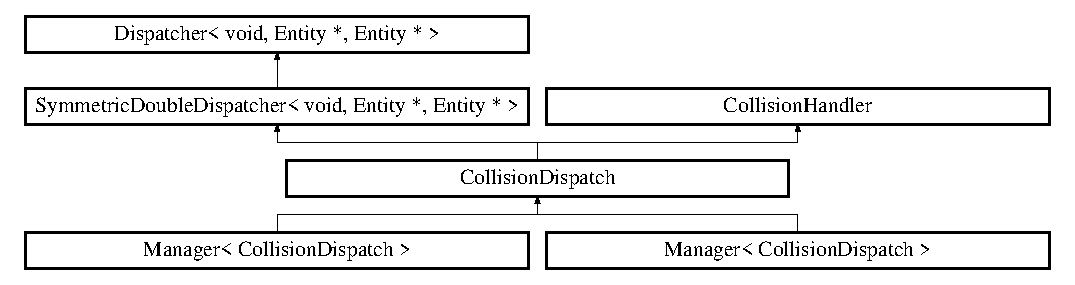
\includegraphics[height=3.383686cm]{class_collision_dispatch}
\end{center}
\end{figure}
\subsection*{Public Member Functions}
\begin{DoxyCompactItemize}
\item 
int \hyperlink{class_collision_dispatch_a11a6867a50874c73098d0744ca3f8bfe}{get\-Rule} (\hyperlink{class_entity}{Entity} $\ast$\-\_\-\-\_\-\-Entity0, \hyperlink{class_entity}{Entity} $\ast$\-\_\-\-\_\-\-Entity1)
\item 
void \hyperlink{class_collision_dispatch_a058bd125ab9bce3aaf054c6cf07381cf}{do\-Rule} (int rulenum, \hyperlink{class_entity}{Entity} $\ast$\-\_\-\-\_\-\-Entity0, \hyperlink{class_entity}{Entity} $\ast$\-\_\-\-\_\-\-Entity1)
\end{DoxyCompactItemize}


\subsection{Member Function Documentation}
\hypertarget{class_collision_dispatch_a058bd125ab9bce3aaf054c6cf07381cf}{\index{Collision\-Dispatch@{Collision\-Dispatch}!do\-Rule@{do\-Rule}}
\index{do\-Rule@{do\-Rule}!CollisionDispatch@{Collision\-Dispatch}}
\subsubsection[{do\-Rule}]{\setlength{\rightskip}{0pt plus 5cm}void Collision\-Dispatch\-::do\-Rule (
\begin{DoxyParamCaption}
\item[{int}]{rulenum, }
\item[{{\bf Entity} $\ast$}]{\-\_\-\-\_\-\-Entity0, }
\item[{{\bf Entity} $\ast$}]{\-\_\-\-\_\-\-Entity1}
\end{DoxyParamCaption}
)}}\label{class_collision_dispatch_a058bd125ab9bce3aaf054c6cf07381cf}
\hypertarget{class_collision_dispatch_a11a6867a50874c73098d0744ca3f8bfe}{\index{Collision\-Dispatch@{Collision\-Dispatch}!get\-Rule@{get\-Rule}}
\index{get\-Rule@{get\-Rule}!CollisionDispatch@{Collision\-Dispatch}}
\subsubsection[{get\-Rule}]{\setlength{\rightskip}{0pt plus 5cm}int Collision\-Dispatch\-::get\-Rule (
\begin{DoxyParamCaption}
\item[{{\bf Entity} $\ast$}]{\-\_\-\-\_\-\-Entity0, }
\item[{{\bf Entity} $\ast$}]{\-\_\-\-\_\-\-Entity1}
\end{DoxyParamCaption}
)}}\label{class_collision_dispatch_a11a6867a50874c73098d0744ca3f8bfe}


The documentation for this class was generated from the following files\-:\begin{DoxyCompactItemize}
\item 
events/dispatch/\hyperlink{dispatchers_8h}{dispatchers.\-h}\item 
events/dispatch/\hyperlink{dispatchers_8cpp}{dispatchers.\-cpp}\end{DoxyCompactItemize}

\hypertarget{class_direction}{\section{Direction Class Reference}
\label{class_direction}\index{Direction@{Direction}}
}


{\ttfamily \#include $<$actions.\-h$>$}

\subsection*{Public Types}
\begin{DoxyCompactItemize}
\item 
enum \hyperlink{class_direction_a218282b2789da5abcafb2be32cf99011}{Dirk} \{ \\*
\hyperlink{class_direction_a218282b2789da5abcafb2be32cf99011a46c48bec0d282018b9d167eef7711b2c}{Dirk\-::up}, 
\hyperlink{class_direction_a218282b2789da5abcafb2be32cf99011a811882fecd5c7618d7099ebbd39ea254}{Dirk\-::left}, 
\hyperlink{class_direction_a218282b2789da5abcafb2be32cf99011a74e8333ad11685ff3bdae589c8f6e34d}{Dirk\-::down}, 
\hyperlink{class_direction_a218282b2789da5abcafb2be32cf99011a7c4f29407893c334a6cb7a87bf045c0d}{Dirk\-::right}, 
\\*
\hyperlink{class_direction_a218282b2789da5abcafb2be32cf99011a7a7229b2be097dd8271879ea690eb5bf}{Dirk\-::no\-\_\-dir}
 \}
\end{DoxyCompactItemize}
\subsection*{Public Member Functions}
\begin{DoxyCompactItemize}
\item 
\hyperlink{class_direction_af17924e019c164609181cdf6bca30397}{Direction} (std\-::string \&s)
\item 
\hyperlink{class_direction_a180839d58bb1ff41301425963701d963}{Direction} (\hyperlink{class_direction_a218282b2789da5abcafb2be32cf99011}{Dirk} d)
\item 
\hyperlink{class_direction_a218282b2789da5abcafb2be32cf99011}{Direction\-::\-Dirk} \hyperlink{class_direction_a8160f7e9bd8442e5a5cc66743c223d1d}{get\-\_\-dir} ()
\item 
void \hyperlink{class_direction_a9ccac2a9f99b9c67cac948bfd99cd366}{move\-\_\-to} (unsigned int \&x, unsigned int \&y)
\item 
void \hyperlink{class_direction_a769ec4b4375d0a78596109005a66eb80}{move\-\_\-from} (unsigned int \&x, unsigned int \&y)
\end{DoxyCompactItemize}
\subsection*{Friends}
\begin{DoxyCompactItemize}
\item 
std\-::ostream \& \hyperlink{class_direction_a81c17e954a272036ec685b1e79b1b006}{operator$<$$<$} (std\-::ostream \&out, \hyperlink{class_direction}{Direction} \&d)
\end{DoxyCompactItemize}


\subsection{Member Enumeration Documentation}
\hypertarget{class_direction_a218282b2789da5abcafb2be32cf99011}{\index{Direction@{Direction}!Dirk@{Dirk}}
\index{Dirk@{Dirk}!Direction@{Direction}}
\subsubsection[{Dirk}]{\setlength{\rightskip}{0pt plus 5cm}enum {\bf Direction\-::\-Dirk}\hspace{0.3cm}{\ttfamily [strong]}}}\label{class_direction_a218282b2789da5abcafb2be32cf99011}
\begin{Desc}
\item[Enumerator]\par
\begin{description}
\index{up@{up}!Direction@{Direction}}\index{Direction@{Direction}!up@{up}}\item[{\em 
\hypertarget{class_direction_a218282b2789da5abcafb2be32cf99011a46c48bec0d282018b9d167eef7711b2c}{up}\label{class_direction_a218282b2789da5abcafb2be32cf99011a46c48bec0d282018b9d167eef7711b2c}
}]\index{left@{left}!Direction@{Direction}}\index{Direction@{Direction}!left@{left}}\item[{\em 
\hypertarget{class_direction_a218282b2789da5abcafb2be32cf99011a811882fecd5c7618d7099ebbd39ea254}{left}\label{class_direction_a218282b2789da5abcafb2be32cf99011a811882fecd5c7618d7099ebbd39ea254}
}]\index{down@{down}!Direction@{Direction}}\index{Direction@{Direction}!down@{down}}\item[{\em 
\hypertarget{class_direction_a218282b2789da5abcafb2be32cf99011a74e8333ad11685ff3bdae589c8f6e34d}{down}\label{class_direction_a218282b2789da5abcafb2be32cf99011a74e8333ad11685ff3bdae589c8f6e34d}
}]\index{right@{right}!Direction@{Direction}}\index{Direction@{Direction}!right@{right}}\item[{\em 
\hypertarget{class_direction_a218282b2789da5abcafb2be32cf99011a7c4f29407893c334a6cb7a87bf045c0d}{right}\label{class_direction_a218282b2789da5abcafb2be32cf99011a7c4f29407893c334a6cb7a87bf045c0d}
}]\index{no\-\_\-dir@{no\-\_\-dir}!Direction@{Direction}}\index{Direction@{Direction}!no\-\_\-dir@{no\-\_\-dir}}\item[{\em 
\hypertarget{class_direction_a218282b2789da5abcafb2be32cf99011a7a7229b2be097dd8271879ea690eb5bf}{no\-\_\-dir}\label{class_direction_a218282b2789da5abcafb2be32cf99011a7a7229b2be097dd8271879ea690eb5bf}
}]\end{description}
\end{Desc}


\subsection{Constructor \& Destructor Documentation}
\hypertarget{class_direction_af17924e019c164609181cdf6bca30397}{\index{Direction@{Direction}!Direction@{Direction}}
\index{Direction@{Direction}!Direction@{Direction}}
\subsubsection[{Direction}]{\setlength{\rightskip}{0pt plus 5cm}Direction\-::\-Direction (
\begin{DoxyParamCaption}
\item[{std\-::string \&}]{s}
\end{DoxyParamCaption}
)}}\label{class_direction_af17924e019c164609181cdf6bca30397}
\hypertarget{class_direction_a180839d58bb1ff41301425963701d963}{\index{Direction@{Direction}!Direction@{Direction}}
\index{Direction@{Direction}!Direction@{Direction}}
\subsubsection[{Direction}]{\setlength{\rightskip}{0pt plus 5cm}Direction\-::\-Direction (
\begin{DoxyParamCaption}
\item[{{\bf Direction\-::\-Dirk}}]{d}
\end{DoxyParamCaption}
)}}\label{class_direction_a180839d58bb1ff41301425963701d963}


\subsection{Member Function Documentation}
\hypertarget{class_direction_a8160f7e9bd8442e5a5cc66743c223d1d}{\index{Direction@{Direction}!get\-\_\-dir@{get\-\_\-dir}}
\index{get\-\_\-dir@{get\-\_\-dir}!Direction@{Direction}}
\subsubsection[{get\-\_\-dir}]{\setlength{\rightskip}{0pt plus 5cm}{\bf Direction\-::\-Dirk} Direction\-::get\-\_\-dir (
\begin{DoxyParamCaption}
{}
\end{DoxyParamCaption}
)}}\label{class_direction_a8160f7e9bd8442e5a5cc66743c223d1d}
\hypertarget{class_direction_a769ec4b4375d0a78596109005a66eb80}{\index{Direction@{Direction}!move\-\_\-from@{move\-\_\-from}}
\index{move\-\_\-from@{move\-\_\-from}!Direction@{Direction}}
\subsubsection[{move\-\_\-from}]{\setlength{\rightskip}{0pt plus 5cm}void Direction\-::move\-\_\-from (
\begin{DoxyParamCaption}
\item[{unsigned int \&}]{x, }
\item[{unsigned int \&}]{y}
\end{DoxyParamCaption}
)}}\label{class_direction_a769ec4b4375d0a78596109005a66eb80}
\hypertarget{class_direction_a9ccac2a9f99b9c67cac948bfd99cd366}{\index{Direction@{Direction}!move\-\_\-to@{move\-\_\-to}}
\index{move\-\_\-to@{move\-\_\-to}!Direction@{Direction}}
\subsubsection[{move\-\_\-to}]{\setlength{\rightskip}{0pt plus 5cm}void Direction\-::move\-\_\-to (
\begin{DoxyParamCaption}
\item[{unsigned int \&}]{x, }
\item[{unsigned int \&}]{y}
\end{DoxyParamCaption}
)}}\label{class_direction_a9ccac2a9f99b9c67cac948bfd99cd366}


\subsection{Friends And Related Function Documentation}
\hypertarget{class_direction_a81c17e954a272036ec685b1e79b1b006}{\index{Direction@{Direction}!operator$<$$<$@{operator$<$$<$}}
\index{operator$<$$<$@{operator$<$$<$}!Direction@{Direction}}
\subsubsection[{operator$<$$<$}]{\setlength{\rightskip}{0pt plus 5cm}std\-::ostream\& operator$<$$<$ (
\begin{DoxyParamCaption}
\item[{std\-::ostream \&}]{out, }
\item[{{\bf Direction} \&}]{d}
\end{DoxyParamCaption}
)\hspace{0.3cm}{\ttfamily [friend]}}}\label{class_direction_a81c17e954a272036ec685b1e79b1b006}


The documentation for this class was generated from the following files\-:\begin{DoxyCompactItemize}
\item 
actions/\hyperlink{actions_8h}{actions.\-h}\item 
actions/\hyperlink{actions_8cpp}{actions.\-cpp}\end{DoxyCompactItemize}

\hypertarget{class_dispatcher}{\section{Dispatcher$<$ Return\-T, Arg\-Base\-Type $>$ Class Template Reference}
\label{class_dispatcher}\index{Dispatcher$<$ Return\-T, Arg\-Base\-Type $>$@{Dispatcher$<$ Return\-T, Arg\-Base\-Type $>$}}
}


{\ttfamily \#include $<$dispatch\-\_\-base.\-h$>$}

\subsection*{Public Member Functions}
\begin{DoxyCompactItemize}
\item 
virtual Return\-T \hyperlink{class_dispatcher_a58db68df090343a88084daa153a19fac}{operator()} (Arg\-Base\-Type...\-args)
\item 
virtual int \hyperlink{class_dispatcher_a2a4ce4aac44e5481bd12c0648837e8f6}{get\-Rule} (Arg\-Base\-Type...\-args)=0
\item 
virtual Return\-T \hyperlink{class_dispatcher_a8d31bba1405451347daad1d1fc66c9c2}{do\-Rule} (int a, Arg\-Base\-Type...\-args)=0
\item 
virtual \hyperlink{class_dispatcher_a344f31cf6aee2eb8401894d44fa0988b}{$\sim$\-Dispatcher} ()
\end{DoxyCompactItemize}


\subsection{Constructor \& Destructor Documentation}
\hypertarget{class_dispatcher_a344f31cf6aee2eb8401894d44fa0988b}{\index{Dispatcher@{Dispatcher}!$\sim$\-Dispatcher@{$\sim$\-Dispatcher}}
\index{$\sim$\-Dispatcher@{$\sim$\-Dispatcher}!Dispatcher@{Dispatcher}}
\subsubsection[{$\sim$\-Dispatcher}]{\setlength{\rightskip}{0pt plus 5cm}template$<$typename Return\-T, typename... Arg\-Base\-Type$>$ virtual {\bf Dispatcher}$<$ Return\-T, Arg\-Base\-Type $>$\-::$\sim${\bf Dispatcher} (
\begin{DoxyParamCaption}
{}
\end{DoxyParamCaption}
)\hspace{0.3cm}{\ttfamily [inline]}, {\ttfamily [virtual]}}}\label{class_dispatcher_a344f31cf6aee2eb8401894d44fa0988b}


\subsection{Member Function Documentation}
\hypertarget{class_dispatcher_a8d31bba1405451347daad1d1fc66c9c2}{\index{Dispatcher@{Dispatcher}!do\-Rule@{do\-Rule}}
\index{do\-Rule@{do\-Rule}!Dispatcher@{Dispatcher}}
\subsubsection[{do\-Rule}]{\setlength{\rightskip}{0pt plus 5cm}template$<$typename Return\-T, typename... Arg\-Base\-Type$>$ virtual Return\-T {\bf Dispatcher}$<$ Return\-T, Arg\-Base\-Type $>$\-::do\-Rule (
\begin{DoxyParamCaption}
\item[{int}]{a, }
\item[{Arg\-Base\-Type...}]{args}
\end{DoxyParamCaption}
)\hspace{0.3cm}{\ttfamily [pure virtual]}}}\label{class_dispatcher_a8d31bba1405451347daad1d1fc66c9c2}
\hypertarget{class_dispatcher_a2a4ce4aac44e5481bd12c0648837e8f6}{\index{Dispatcher@{Dispatcher}!get\-Rule@{get\-Rule}}
\index{get\-Rule@{get\-Rule}!Dispatcher@{Dispatcher}}
\subsubsection[{get\-Rule}]{\setlength{\rightskip}{0pt plus 5cm}template$<$typename Return\-T, typename... Arg\-Base\-Type$>$ virtual int {\bf Dispatcher}$<$ Return\-T, Arg\-Base\-Type $>$\-::get\-Rule (
\begin{DoxyParamCaption}
\item[{Arg\-Base\-Type...}]{args}
\end{DoxyParamCaption}
)\hspace{0.3cm}{\ttfamily [pure virtual]}}}\label{class_dispatcher_a2a4ce4aac44e5481bd12c0648837e8f6}
\hypertarget{class_dispatcher_a58db68df090343a88084daa153a19fac}{\index{Dispatcher@{Dispatcher}!operator()@{operator()}}
\index{operator()@{operator()}!Dispatcher@{Dispatcher}}
\subsubsection[{operator()}]{\setlength{\rightskip}{0pt plus 5cm}template$<$typename Return\-T, typename... Arg\-Base\-Type$>$ virtual Return\-T {\bf Dispatcher}$<$ Return\-T, Arg\-Base\-Type $>$\-::operator() (
\begin{DoxyParamCaption}
\item[{Arg\-Base\-Type...}]{args}
\end{DoxyParamCaption}
)\hspace{0.3cm}{\ttfamily [inline]}, {\ttfamily [virtual]}}}\label{class_dispatcher_a58db68df090343a88084daa153a19fac}


The documentation for this class was generated from the following file\-:\begin{DoxyCompactItemize}
\item 
events/dispatch/\hyperlink{dispatch__base_8h}{dispatch\-\_\-base.\-h}\end{DoxyCompactItemize}

\hypertarget{class_entity}{\section{Entity Class Reference}
\label{class_entity}\index{Entity@{Entity}}
}


{\ttfamily \#include $<$entity.\-h$>$}

Inheritance diagram for Entity\-:\begin{figure}[H]
\begin{center}
\leavevmode
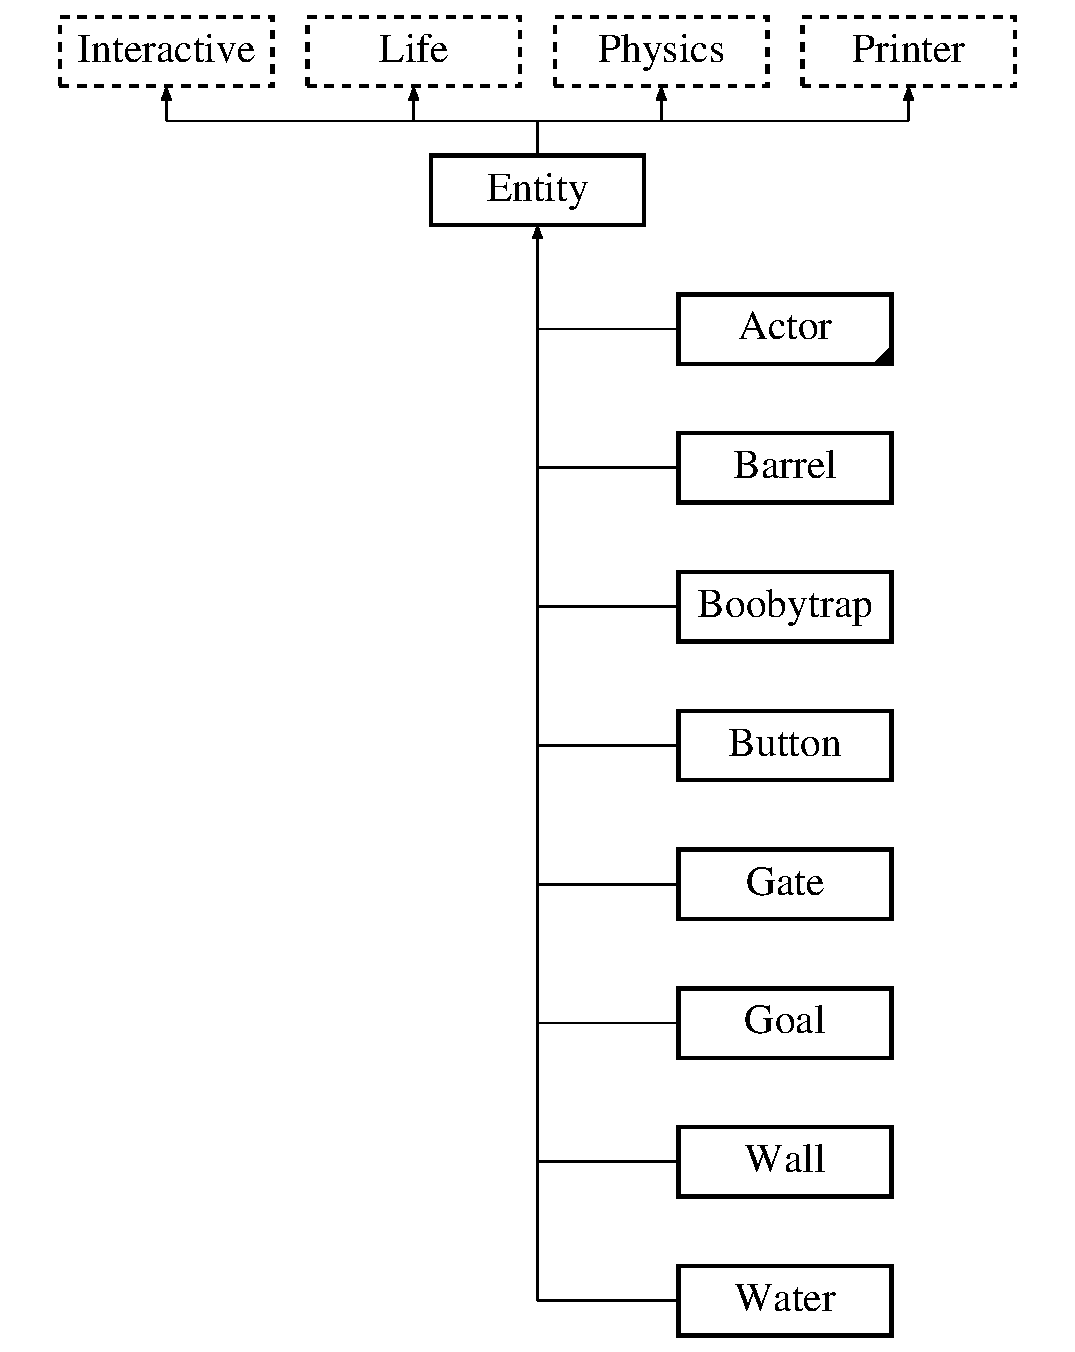
\includegraphics[height=10.000000cm]{class_entity}
\end{center}
\end{figure}
\subsection*{Public Member Functions}
\begin{DoxyCompactItemize}
\item 
virtual void \hyperlink{class_entity_a11d5655c6e057fb86551402380009c01}{\-\_\-\-\_\-polymorphic\-\_\-\-\_\-} ()
\item 
\hyperlink{class_entity_a0a44f1b08b1c84fef9d62a2e12e5af14}{Entity} (unsigned int \-\_\-x, unsigned int \-\_\-y)
\item 
\hyperlink{class_entity_ac565cb6d4e6d9dc40c910809c83e5dfe}{Entity} (const \hyperlink{class_entity}{Entity} \&that)
\begin{DoxyCompactList}\small\item\em Copy constructor. \end{DoxyCompactList}\item 
\hyperlink{class_entity}{Entity} \& \hyperlink{class_entity_a5f8e38834cf2661b2edf50b62fa8d8b8}{operator=} (const \hyperlink{class_entity}{Entity} \&that)
\begin{DoxyCompactList}\small\item\em Copy by assignment. \end{DoxyCompactList}\item 
virtual void \hyperlink{class_entity_aa694874d1f59971187de675d1e0c1fdf}{info} (std\-::ostream \&out)=0
\item 
virtual \hyperlink{class_entity_a588098978eea6a3486b7361605ff3f0f}{$\sim$\-Entity} ()
\item 
bool \hyperlink{class_entity_af7f20142aa7883ca29a91c43e3511e48}{properly\-Initialized} ()
\end{DoxyCompactItemize}
\subsection*{Public Attributes}
\begin{DoxyCompactItemize}
\item 
unsigned int \hyperlink{class_entity_afa8f48eccdb09a290e2c1ded3f135363}{x}
\item 
unsigned int \hyperlink{class_entity_a9d39843430829a89bb8233dbaadae4f1}{y}
\end{DoxyCompactItemize}


\subsection{Constructor \& Destructor Documentation}
\hypertarget{class_entity_a0a44f1b08b1c84fef9d62a2e12e5af14}{\index{Entity@{Entity}!Entity@{Entity}}
\index{Entity@{Entity}!Entity@{Entity}}
\subsubsection[{Entity}]{\setlength{\rightskip}{0pt plus 5cm}Entity\-::\-Entity (
\begin{DoxyParamCaption}
\item[{unsigned int}]{\-\_\-x, }
\item[{unsigned int}]{\-\_\-y}
\end{DoxyParamCaption}
)}}\label{class_entity_a0a44f1b08b1c84fef9d62a2e12e5af14}
E\-N\-S\-U\-R\-E(\hyperlink{class_entity_af7f20142aa7883ca29a91c43e3511e48}{properly\-Initialized()}, \char`\"{}\-Constructor must end...\char`\"{}) \hypertarget{class_entity_ac565cb6d4e6d9dc40c910809c83e5dfe}{\index{Entity@{Entity}!Entity@{Entity}}
\index{Entity@{Entity}!Entity@{Entity}}
\subsubsection[{Entity}]{\setlength{\rightskip}{0pt plus 5cm}Entity\-::\-Entity (
\begin{DoxyParamCaption}
\item[{const {\bf Entity} \&}]{that}
\end{DoxyParamCaption}
)}}\label{class_entity_ac565cb6d4e6d9dc40c910809c83e5dfe}


Copy constructor. 

E\-N\-S\-U\-R\-E(\hyperlink{class_entity_af7f20142aa7883ca29a91c43e3511e48}{properly\-Initialized()}, \char`\"{}\-Copy constructor must end...\char`\"{}) \hypertarget{class_entity_a588098978eea6a3486b7361605ff3f0f}{\index{Entity@{Entity}!$\sim$\-Entity@{$\sim$\-Entity}}
\index{$\sim$\-Entity@{$\sim$\-Entity}!Entity@{Entity}}
\subsubsection[{$\sim$\-Entity}]{\setlength{\rightskip}{0pt plus 5cm}virtual Entity\-::$\sim$\-Entity (
\begin{DoxyParamCaption}
{}
\end{DoxyParamCaption}
)\hspace{0.3cm}{\ttfamily [inline]}, {\ttfamily [virtual]}}}\label{class_entity_a588098978eea6a3486b7361605ff3f0f}


\subsection{Member Function Documentation}
\hypertarget{class_entity_a11d5655c6e057fb86551402380009c01}{\index{Entity@{Entity}!\-\_\-\-\_\-polymorphic\-\_\-\-\_\-@{\-\_\-\-\_\-polymorphic\-\_\-\-\_\-}}
\index{\-\_\-\-\_\-polymorphic\-\_\-\-\_\-@{\-\_\-\-\_\-polymorphic\-\_\-\-\_\-}!Entity@{Entity}}
\subsubsection[{\-\_\-\-\_\-polymorphic\-\_\-\-\_\-}]{\setlength{\rightskip}{0pt plus 5cm}virtual void Entity\-::\-\_\-\-\_\-polymorphic\-\_\-\-\_\- (
\begin{DoxyParamCaption}
{}
\end{DoxyParamCaption}
)\hspace{0.3cm}{\ttfamily [inline]}, {\ttfamily [virtual]}}}\label{class_entity_a11d5655c6e057fb86551402380009c01}


Reimplemented from \hyperlink{class_interactive_a07537d2f82f4b05daaa9abfe24e16673}{Interactive}.

\hypertarget{class_entity_aa694874d1f59971187de675d1e0c1fdf}{\index{Entity@{Entity}!info@{info}}
\index{info@{info}!Entity@{Entity}}
\subsubsection[{info}]{\setlength{\rightskip}{0pt plus 5cm}virtual void Entity\-::info (
\begin{DoxyParamCaption}
\item[{std\-::ostream \&}]{out}
\end{DoxyParamCaption}
)\hspace{0.3cm}{\ttfamily [pure virtual]}}}\label{class_entity_aa694874d1f59971187de675d1e0c1fdf}
Shows the info about the entity, used in the method \hyperlink{class_board_ae7e407126c1c113669e645a216fc7848}{Board\-::write\-\_\-board}. Is a pure virtual function for \hyperlink{class_entity}{Entity}. R\-E\-Q\-U\-I\-R\-E(\hyperlink{class_entity_af7f20142aa7883ca29a91c43e3511e48}{properly\-Initialized()}, \char`\"{}\-Entity wasn't initialized when calling info\char`\"{}) 

Implemented in \hyperlink{class_gate_a194b57934f4ab3ed226a7c5fb45693bd}{Gate}, \hyperlink{class_button_aba3d89d8caf373ced3f69f24ad09682a}{Button}, \hyperlink{class_water_a0931381448954bfc525aa6492860f599}{Water}, \hyperlink{class_barrel_aebd6e6fda845b455a01d4731286cee67}{Barrel}, \hyperlink{class_boobytrap_aa73f3cbd8027a4ae55e082a62971ef72}{Boobytrap}, \hyperlink{class_goal_adbce7419324f805e9b0527d85d033ce2}{Goal}, \hyperlink{class_wall_a0ff5e8bb39976f825e99dcd51a2ee610}{Wall}, \hyperlink{class_monster_aba6f66599146c238ff906e0bffb06b71}{Monster}, and \hyperlink{class_player_a43124e562ec95ecd4a2aece053b65098}{Player}.

\hypertarget{class_entity_a5f8e38834cf2661b2edf50b62fa8d8b8}{\index{Entity@{Entity}!operator=@{operator=}}
\index{operator=@{operator=}!Entity@{Entity}}
\subsubsection[{operator=}]{\setlength{\rightskip}{0pt plus 5cm}{\bf Entity} \& Entity\-::operator= (
\begin{DoxyParamCaption}
\item[{const {\bf Entity} \&}]{that}
\end{DoxyParamCaption}
)}}\label{class_entity_a5f8e38834cf2661b2edf50b62fa8d8b8}


Copy by assignment. 

E\-N\-S\-U\-R\-E(\hyperlink{class_entity_af7f20142aa7883ca29a91c43e3511e48}{properly\-Initialized()}, \char`\"{}\-Copy by assignment must end...\char`\"{}) \hypertarget{class_entity_af7f20142aa7883ca29a91c43e3511e48}{\index{Entity@{Entity}!properly\-Initialized@{properly\-Initialized}}
\index{properly\-Initialized@{properly\-Initialized}!Entity@{Entity}}
\subsubsection[{properly\-Initialized}]{\setlength{\rightskip}{0pt plus 5cm}bool Entity\-::properly\-Initialized (
\begin{DoxyParamCaption}
{}
\end{DoxyParamCaption}
)}}\label{class_entity_af7f20142aa7883ca29a91c43e3511e48}


\subsection{Member Data Documentation}
\hypertarget{class_entity_afa8f48eccdb09a290e2c1ded3f135363}{\index{Entity@{Entity}!x@{x}}
\index{x@{x}!Entity@{Entity}}
\subsubsection[{x}]{\setlength{\rightskip}{0pt plus 5cm}unsigned int Entity\-::x}}\label{class_entity_afa8f48eccdb09a290e2c1ded3f135363}
\hypertarget{class_entity_a9d39843430829a89bb8233dbaadae4f1}{\index{Entity@{Entity}!y@{y}}
\index{y@{y}!Entity@{Entity}}
\subsubsection[{y}]{\setlength{\rightskip}{0pt plus 5cm}unsigned int Entity\-::y}}\label{class_entity_a9d39843430829a89bb8233dbaadae4f1}


The documentation for this class was generated from the following files\-:\begin{DoxyCompactItemize}
\item 
entities/\hyperlink{entity_8h}{entity.\-h}\item 
entities/\hyperlink{entity_8cpp}{entity.\-cpp}\end{DoxyCompactItemize}

\hypertarget{classconvert_1_1_entity}{\section{convert.\-Entity Class Reference}
\label{classconvert_1_1_entity}\index{convert.\-Entity@{convert.\-Entity}}
}
\subsection*{Public Member Functions}
\begin{DoxyCompactItemize}
\item 
def \hyperlink{classconvert_1_1_entity_a39a85148567346bf092994df1aeb5f43}{\-\_\-\-\_\-init\-\_\-\-\_\-}
\item 
def \hyperlink{classconvert_1_1_entity_aa71aa733a4e55feec1d0a33773f98b71}{new\-\_\-format}
\end{DoxyCompactItemize}
\subsection*{Public Attributes}
\begin{DoxyCompactItemize}
\item 
\hyperlink{classconvert_1_1_entity_a80eb3f8a523f2f82bce7714aa64dd4e9}{x}
\item 
\hyperlink{classconvert_1_1_entity_adce59aac5a6f84b4eed9afc72737e11e}{y}
\item 
\hyperlink{classconvert_1_1_entity_a78936a04ea3735de546ffa877b2ad02d}{beweegbaar}
\item 
\hyperlink{classconvert_1_1_entity_a050e99f5fa3fa332ec1890b0c7ce165f}{typ}
\item 
\hyperlink{classconvert_1_1_entity_a0c8f63ae0353069137abe9a8e4c9b112}{subs}
\end{DoxyCompactItemize}


\subsection{Constructor \& Destructor Documentation}
\hypertarget{classconvert_1_1_entity_a39a85148567346bf092994df1aeb5f43}{\index{convert\-::\-Entity@{convert\-::\-Entity}!\-\_\-\-\_\-init\-\_\-\-\_\-@{\-\_\-\-\_\-init\-\_\-\-\_\-}}
\index{\-\_\-\-\_\-init\-\_\-\-\_\-@{\-\_\-\-\_\-init\-\_\-\-\_\-}!convert::Entity@{convert\-::\-Entity}}
\subsubsection[{\-\_\-\-\_\-init\-\_\-\-\_\-}]{\setlength{\rightskip}{0pt plus 5cm}def convert.\-Entity.\-\_\-\-\_\-init\-\_\-\-\_\- (
\begin{DoxyParamCaption}
\item[{}]{self, }
\item[{}]{el}
\end{DoxyParamCaption}
)}}\label{classconvert_1_1_entity_a39a85148567346bf092994df1aeb5f43}


\subsection{Member Function Documentation}
\hypertarget{classconvert_1_1_entity_aa71aa733a4e55feec1d0a33773f98b71}{\index{convert\-::\-Entity@{convert\-::\-Entity}!new\-\_\-format@{new\-\_\-format}}
\index{new\-\_\-format@{new\-\_\-format}!convert::Entity@{convert\-::\-Entity}}
\subsubsection[{new\-\_\-format}]{\setlength{\rightskip}{0pt plus 5cm}def convert.\-Entity.\-new\-\_\-format (
\begin{DoxyParamCaption}
\item[{}]{self}
\end{DoxyParamCaption}
)}}\label{classconvert_1_1_entity_aa71aa733a4e55feec1d0a33773f98b71}


\subsection{Member Data Documentation}
\hypertarget{classconvert_1_1_entity_a78936a04ea3735de546ffa877b2ad02d}{\index{convert\-::\-Entity@{convert\-::\-Entity}!beweegbaar@{beweegbaar}}
\index{beweegbaar@{beweegbaar}!convert::Entity@{convert\-::\-Entity}}
\subsubsection[{beweegbaar}]{\setlength{\rightskip}{0pt plus 5cm}convert.\-Entity.\-beweegbaar}}\label{classconvert_1_1_entity_a78936a04ea3735de546ffa877b2ad02d}
\hypertarget{classconvert_1_1_entity_a0c8f63ae0353069137abe9a8e4c9b112}{\index{convert\-::\-Entity@{convert\-::\-Entity}!subs@{subs}}
\index{subs@{subs}!convert::Entity@{convert\-::\-Entity}}
\subsubsection[{subs}]{\setlength{\rightskip}{0pt plus 5cm}convert.\-Entity.\-subs}}\label{classconvert_1_1_entity_a0c8f63ae0353069137abe9a8e4c9b112}
\hypertarget{classconvert_1_1_entity_a050e99f5fa3fa332ec1890b0c7ce165f}{\index{convert\-::\-Entity@{convert\-::\-Entity}!typ@{typ}}
\index{typ@{typ}!convert::Entity@{convert\-::\-Entity}}
\subsubsection[{typ}]{\setlength{\rightskip}{0pt plus 5cm}convert.\-Entity.\-typ}}\label{classconvert_1_1_entity_a050e99f5fa3fa332ec1890b0c7ce165f}
\hypertarget{classconvert_1_1_entity_a80eb3f8a523f2f82bce7714aa64dd4e9}{\index{convert\-::\-Entity@{convert\-::\-Entity}!x@{x}}
\index{x@{x}!convert::Entity@{convert\-::\-Entity}}
\subsubsection[{x}]{\setlength{\rightskip}{0pt plus 5cm}convert.\-Entity.\-x}}\label{classconvert_1_1_entity_a80eb3f8a523f2f82bce7714aa64dd4e9}
\hypertarget{classconvert_1_1_entity_adce59aac5a6f84b4eed9afc72737e11e}{\index{convert\-::\-Entity@{convert\-::\-Entity}!y@{y}}
\index{y@{y}!convert::Entity@{convert\-::\-Entity}}
\subsubsection[{y}]{\setlength{\rightskip}{0pt plus 5cm}convert.\-Entity.\-y}}\label{classconvert_1_1_entity_adce59aac5a6f84b4eed9afc72737e11e}


The documentation for this class was generated from the following file\-:\begin{DoxyCompactItemize}
\item 
tests/filetests\-\_\-old/\hyperlink{convert_8py}{convert.\-py}\end{DoxyCompactItemize}

\hypertarget{class_entity__parser}{\section{Entity\-\_\-parser Class Reference}
\label{class_entity__parser}\index{Entity\-\_\-parser@{Entity\-\_\-parser}}
}


{\ttfamily \#include $<$entity\-\_\-parser.\-h$>$}

Inheritance diagram for Entity\-\_\-parser\-:\begin{figure}[H]
\begin{center}
\leavevmode
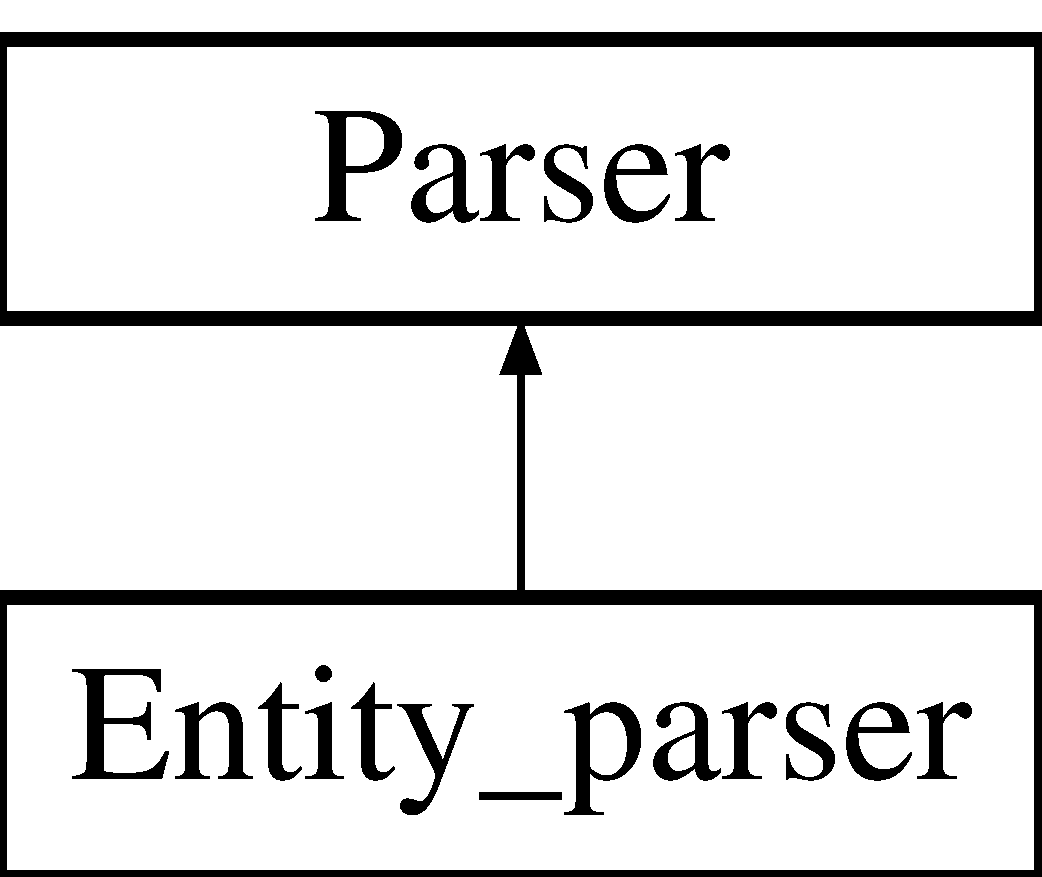
\includegraphics[height=2.000000cm]{class_entity__parser}
\end{center}
\end{figure}
\subsection*{Public Member Functions}
\begin{DoxyCompactItemize}
\item 
\hyperlink{class_entity__parser_ae71a89ee9d79647da978187f08c69b33}{Entity\-\_\-parser} (std\-::ostream $\ast$stream, std\-::string filename)
\item 
\hyperlink{class_entity__parser_a3efc9df13b6fd109315f4c6f36a76375}{Entity\-\_\-parser} ()=default
\item 
\hyperlink{class_wall}{Wall} $\ast$ \hyperlink{class_entity__parser_a4b5ec7aef90947d346db9cf6aeb8fe6b}{parse\-\_\-wall} (Ti\-Xml\-Element $\ast$elem, \hyperlink{class_board}{Board} \&\-\_\-board)
\item 
\hyperlink{class_barrel}{Barrel} $\ast$ \hyperlink{class_entity__parser_ac6460766a3fb0fb8a54e59f1a09c02f2}{parse\-\_\-barrel} (Ti\-Xml\-Element $\ast$elem, \hyperlink{class_board}{Board} \&\-\_\-board)
\item 
\hyperlink{class_water}{Water} $\ast$ \hyperlink{class_entity__parser_ab337768346e511822f49418ceb7a3549}{parse\-\_\-water} (Ti\-Xml\-Element $\ast$elem, \hyperlink{class_board}{Board} \&\-\_\-board)
\item 
\hyperlink{class_button}{Button} $\ast$ \hyperlink{class_entity__parser_a2c2da316e966ba3ac64d18874a4cd274}{parse\-\_\-button} (Ti\-Xml\-Element $\ast$elem, \hyperlink{class_board}{Board} \&\-\_\-board)
\item 
\hyperlink{class_goal}{Goal} $\ast$ \hyperlink{class_entity__parser_af9188db166e12f5def2c4423d259a57c}{parse\-\_\-goal} (Ti\-Xml\-Element $\ast$elem, \hyperlink{class_board}{Board} \&\-\_\-board)
\item 
\hyperlink{class_boobytrap}{Boobytrap} $\ast$ \hyperlink{class_entity__parser_ac1e5914d94309fe88069b1e8a5c071db}{parse\-\_\-boobytrap} (Ti\-Xml\-Element $\ast$elem, \hyperlink{class_board}{Board} \&\-\_\-board)
\item 
\hyperlink{class_gate}{Gate} $\ast$ \hyperlink{class_entity__parser_ab85fb730a2a1c07539aed278f204010b}{parse\-\_\-gate} (Ti\-Xml\-Element $\ast$elem, \hyperlink{class_board}{Board} \&\-\_\-board)
\end{DoxyCompactItemize}
\subsection*{Additional Inherited Members}


\subsection{Constructor \& Destructor Documentation}
\hypertarget{class_entity__parser_ae71a89ee9d79647da978187f08c69b33}{\index{Entity\-\_\-parser@{Entity\-\_\-parser}!Entity\-\_\-parser@{Entity\-\_\-parser}}
\index{Entity\-\_\-parser@{Entity\-\_\-parser}!Entity_parser@{Entity\-\_\-parser}}
\subsubsection[{Entity\-\_\-parser}]{\setlength{\rightskip}{0pt plus 5cm}Entity\-\_\-parser\-::\-Entity\-\_\-parser (
\begin{DoxyParamCaption}
\item[{std\-::ostream $\ast$}]{stream, }
\item[{std\-::string}]{filename}
\end{DoxyParamCaption}
)}}\label{class_entity__parser_ae71a89ee9d79647da978187f08c69b33}
\hypertarget{class_entity__parser_a3efc9df13b6fd109315f4c6f36a76375}{\index{Entity\-\_\-parser@{Entity\-\_\-parser}!Entity\-\_\-parser@{Entity\-\_\-parser}}
\index{Entity\-\_\-parser@{Entity\-\_\-parser}!Entity_parser@{Entity\-\_\-parser}}
\subsubsection[{Entity\-\_\-parser}]{\setlength{\rightskip}{0pt plus 5cm}Entity\-\_\-parser\-::\-Entity\-\_\-parser (
\begin{DoxyParamCaption}
{}
\end{DoxyParamCaption}
)\hspace{0.3cm}{\ttfamily [default]}}}\label{class_entity__parser_a3efc9df13b6fd109315f4c6f36a76375}


\subsection{Member Function Documentation}
\hypertarget{class_entity__parser_ac6460766a3fb0fb8a54e59f1a09c02f2}{\index{Entity\-\_\-parser@{Entity\-\_\-parser}!parse\-\_\-barrel@{parse\-\_\-barrel}}
\index{parse\-\_\-barrel@{parse\-\_\-barrel}!Entity_parser@{Entity\-\_\-parser}}
\subsubsection[{parse\-\_\-barrel}]{\setlength{\rightskip}{0pt plus 5cm}{\bf Barrel} $\ast$ Entity\-\_\-parser\-::parse\-\_\-barrel (
\begin{DoxyParamCaption}
\item[{Ti\-Xml\-Element $\ast$}]{elem, }
\item[{{\bf Board} \&}]{\-\_\-board}
\end{DoxyParamCaption}
)}}\label{class_entity__parser_ac6460766a3fb0fb8a54e59f1a09c02f2}
\hypertarget{class_entity__parser_ac1e5914d94309fe88069b1e8a5c071db}{\index{Entity\-\_\-parser@{Entity\-\_\-parser}!parse\-\_\-boobytrap@{parse\-\_\-boobytrap}}
\index{parse\-\_\-boobytrap@{parse\-\_\-boobytrap}!Entity_parser@{Entity\-\_\-parser}}
\subsubsection[{parse\-\_\-boobytrap}]{\setlength{\rightskip}{0pt plus 5cm}{\bf Boobytrap} $\ast$ Entity\-\_\-parser\-::parse\-\_\-boobytrap (
\begin{DoxyParamCaption}
\item[{Ti\-Xml\-Element $\ast$}]{elem, }
\item[{{\bf Board} \&}]{\-\_\-board}
\end{DoxyParamCaption}
)}}\label{class_entity__parser_ac1e5914d94309fe88069b1e8a5c071db}
\hypertarget{class_entity__parser_a2c2da316e966ba3ac64d18874a4cd274}{\index{Entity\-\_\-parser@{Entity\-\_\-parser}!parse\-\_\-button@{parse\-\_\-button}}
\index{parse\-\_\-button@{parse\-\_\-button}!Entity_parser@{Entity\-\_\-parser}}
\subsubsection[{parse\-\_\-button}]{\setlength{\rightskip}{0pt plus 5cm}{\bf Button} $\ast$ Entity\-\_\-parser\-::parse\-\_\-button (
\begin{DoxyParamCaption}
\item[{Ti\-Xml\-Element $\ast$}]{elem, }
\item[{{\bf Board} \&}]{\-\_\-board}
\end{DoxyParamCaption}
)}}\label{class_entity__parser_a2c2da316e966ba3ac64d18874a4cd274}
\hypertarget{class_entity__parser_ab85fb730a2a1c07539aed278f204010b}{\index{Entity\-\_\-parser@{Entity\-\_\-parser}!parse\-\_\-gate@{parse\-\_\-gate}}
\index{parse\-\_\-gate@{parse\-\_\-gate}!Entity_parser@{Entity\-\_\-parser}}
\subsubsection[{parse\-\_\-gate}]{\setlength{\rightskip}{0pt plus 5cm}{\bf Gate} $\ast$ Entity\-\_\-parser\-::parse\-\_\-gate (
\begin{DoxyParamCaption}
\item[{Ti\-Xml\-Element $\ast$}]{elem, }
\item[{{\bf Board} \&}]{\-\_\-board}
\end{DoxyParamCaption}
)}}\label{class_entity__parser_ab85fb730a2a1c07539aed278f204010b}
\hypertarget{class_entity__parser_af9188db166e12f5def2c4423d259a57c}{\index{Entity\-\_\-parser@{Entity\-\_\-parser}!parse\-\_\-goal@{parse\-\_\-goal}}
\index{parse\-\_\-goal@{parse\-\_\-goal}!Entity_parser@{Entity\-\_\-parser}}
\subsubsection[{parse\-\_\-goal}]{\setlength{\rightskip}{0pt plus 5cm}{\bf Goal} $\ast$ Entity\-\_\-parser\-::parse\-\_\-goal (
\begin{DoxyParamCaption}
\item[{Ti\-Xml\-Element $\ast$}]{elem, }
\item[{{\bf Board} \&}]{\-\_\-board}
\end{DoxyParamCaption}
)}}\label{class_entity__parser_af9188db166e12f5def2c4423d259a57c}
\hypertarget{class_entity__parser_a4b5ec7aef90947d346db9cf6aeb8fe6b}{\index{Entity\-\_\-parser@{Entity\-\_\-parser}!parse\-\_\-wall@{parse\-\_\-wall}}
\index{parse\-\_\-wall@{parse\-\_\-wall}!Entity_parser@{Entity\-\_\-parser}}
\subsubsection[{parse\-\_\-wall}]{\setlength{\rightskip}{0pt plus 5cm}{\bf Wall} $\ast$ Entity\-\_\-parser\-::parse\-\_\-wall (
\begin{DoxyParamCaption}
\item[{Ti\-Xml\-Element $\ast$}]{elem, }
\item[{{\bf Board} \&}]{\-\_\-board}
\end{DoxyParamCaption}
)}}\label{class_entity__parser_a4b5ec7aef90947d346db9cf6aeb8fe6b}
\hypertarget{class_entity__parser_ab337768346e511822f49418ceb7a3549}{\index{Entity\-\_\-parser@{Entity\-\_\-parser}!parse\-\_\-water@{parse\-\_\-water}}
\index{parse\-\_\-water@{parse\-\_\-water}!Entity_parser@{Entity\-\_\-parser}}
\subsubsection[{parse\-\_\-water}]{\setlength{\rightskip}{0pt plus 5cm}{\bf Water} $\ast$ Entity\-\_\-parser\-::parse\-\_\-water (
\begin{DoxyParamCaption}
\item[{Ti\-Xml\-Element $\ast$}]{elem, }
\item[{{\bf Board} \&}]{\-\_\-board}
\end{DoxyParamCaption}
)}}\label{class_entity__parser_ab337768346e511822f49418ceb7a3549}


The documentation for this class was generated from the following files\-:\begin{DoxyCompactItemize}
\item 
parsers/\hyperlink{entity__parser_8h}{entity\-\_\-parser.\-h}\item 
parsers/\hyperlink{entity__parser_8cpp}{entity\-\_\-parser.\-cpp}\end{DoxyCompactItemize}

\hypertarget{class_game}{\section{Game Class Reference}
\label{class_game}\index{Game@{Game}}
}


{\ttfamily \#include $<$game.\-h$>$}

\subsection*{Public Types}
\begin{DoxyCompactItemize}
\item 
typedef std\-::map$<$ std\-::string, \\*
\hyperlink{class_player}{Player} $\ast$ $>$ \hyperlink{class_game_a11e553861e3a7fc842680e55171ed06f}{Playermap}
\item 
typedef std\-::map$<$ std\-::string, \\*
\hyperlink{class_monster}{Monster} $\ast$ $>$ \hyperlink{class_game_a2c39481e575abd66baa206771c504149}{Monstermap}
\item 
typedef std\-::map$<$ std\-::string, \\*
\hyperlink{class_gate}{Gate} $\ast$ $>$ \hyperlink{class_game_a3ac788aaa1e70509a9b9745acd17a8b5}{Gatemap}
\end{DoxyCompactItemize}
\subsection*{Public Member Functions}
\begin{DoxyCompactItemize}
\item 
\hyperlink{class_game_ad59df6562a58a614fda24622d3715b65}{Game} ()
\item 
\hyperlink{class_player}{Player} $\ast$ \hyperlink{class_game_aeccd4cec699287294ff72399eea97bf8}{get\-\_\-player} (std\-::string \&name)
\item 
\hyperlink{class_monster}{Monster} $\ast$ \hyperlink{class_game_a84d0739f97b1d522c1c5739f1cef3e75}{get\-\_\-monster} (std\-::string \&name)
\item 
\hyperlink{class_actor}{Actor} $\ast$ \hyperlink{class_game_aa0e2afd92f042ebbc3635c05d8c2a412}{get\-\_\-actor} (std\-::string \&name)
\item 
\hyperlink{class_gate}{Gate} $\ast$ \hyperlink{class_game_af381f79ab245cb6075797323ccf730c1}{get\-\_\-gate} (std\-::string \&name)
\item 
void \hyperlink{class_game_a532e7897423e470019ada16917b457c2}{add\-\_\-player} (\hyperlink{class_player}{Player} $\ast$p)
\item 
void \hyperlink{class_game_a5b3ceb773fe5f462bb23679ed0482db1}{add\-\_\-monster} (\hyperlink{class_monster}{Monster} $\ast$m)
\item 
void \hyperlink{class_game_a2b5f926b163ba9ff405f45c5f3e7d734}{add\-\_\-gate} (\hyperlink{class_gate}{Gate} $\ast$g)
\item 
void \hyperlink{class_game_a73b72d3098c7c9a8d232b5fd4b1139ad}{write\-\_\-actions} (std\-::ostream \&out)
\item 
int \hyperlink{class_game_ad6165e671cd454ac4c2296f306d293eb}{players\-\_\-alive} ()
\item 
void \hyperlink{class_game_a1845d7f4c11f16a76e79f119f4077f17}{bury} (\hyperlink{class_entity}{Entity} $\ast$e)
\item 
void \hyperlink{class_game_a8f72aa6ced41ae11bdaa48ef73d11d39}{do\-\_\-all\-\_\-actions} (std\-::ostream \&out)
\item 
void \hyperlink{class_game_aba0acb0d0ec55e050440e9f398de773c}{do\-\_\-action} (std\-::ostream \&out)
\item 
int \hyperlink{class_game_aeb84d2cc01cb7e69e82a92bb41221d3e}{get\-\_\-num\-\_\-actions} ()
\item 
bool \hyperlink{class_game_a47be91dcc180c606507cc06d06d351b2}{is\-\_\-ended} ()
\item 
void \hyperlink{class_game_aeab39f9bf569d983f6163add6706ad82}{clear\-\_\-actions} ()
\item 
\hyperlink{class_board}{Board} $\ast$ \hyperlink{class_game_a6f66f42cdc7be06668ac60bff23db9d9}{get\-\_\-board} ()
\item 
void \hyperlink{class_game_ac164df696f1b71acc6246a08e8066b70}{set\-\_\-board} (\hyperlink{class_board}{Board} $\ast$b)
\item 
void \hyperlink{class_game_ad37c165fa3af0658bec23511f57785db}{kill} (\hyperlink{class_entity}{Entity} $\ast$a)
\item 
void \hyperlink{class_game_a3eca6db94a95d5fa843ba69a142a62bb}{collide} (\hyperlink{class_entity}{Entity} $\ast$a, \hyperlink{class_entity}{Entity} $\ast$b)
\item 
void \hyperlink{class_game_a0cc9604134dde3c5e80cebdc97a270e1}{enter} (\hyperlink{class_entity}{Entity} $\ast$top, \hyperlink{class_entity}{Entity} $\ast$bottom)
\item 
void \hyperlink{class_game_a737c0a9f00bccef6f3e8e743a2f8bea1}{leave} (\hyperlink{class_entity}{Entity} $\ast$top, \hyperlink{class_entity}{Entity} $\ast$bottom)
\item 
\hyperlink{class_game_ae3d112ca6e0e55150d2fdbc704474530}{$\sim$\-Game} ()
\item 
bool \hyperlink{class_game_a7a97d89e85982b7d67d13e0c502de6a2}{properly\-Initialized} ()
\end{DoxyCompactItemize}
\subsection*{Public Attributes}
\begin{DoxyCompactItemize}
\item 
std\-::list$<$ \hyperlink{class_action}{Action} $\ast$ $>$ \hyperlink{class_game_a8e61c60693aa39b8a3deb5f3f277b43f}{actions}
\end{DoxyCompactItemize}
\subsection*{Friends}
\begin{DoxyCompactItemize}
\item 
class \hyperlink{class_game_ab0955901615f29e137d1ad6b95fc2c55}{Collision\-Handler}
\item 
class \hyperlink{class_game_ad46435fe6b8e9a384d33d608058862ae}{I\-A\-\_\-\-Enter\-Handler}
\item 
class \hyperlink{class_game_adc4c20007ad2fd4bc2556fbfbff54945}{I\-A\-\_\-\-Leave\-Handler}
\item 
class \hyperlink{class_game_aab5a016b7fd0a16c4e689d3102ec3a17}{Kill\-Handler}
\item 
class \hyperlink{class_game_a12525b6ed7c8186be0bee5cf78e2a49c}{Board}
\end{DoxyCompactItemize}


\subsection{Member Typedef Documentation}
\hypertarget{class_game_a3ac788aaa1e70509a9b9745acd17a8b5}{\index{Game@{Game}!Gatemap@{Gatemap}}
\index{Gatemap@{Gatemap}!Game@{Game}}
\subsubsection[{Gatemap}]{\setlength{\rightskip}{0pt plus 5cm}typedef std\-::map$<$std\-::string, {\bf Gate}$\ast$$>$ {\bf Game\-::\-Gatemap}}}\label{class_game_a3ac788aaa1e70509a9b9745acd17a8b5}
\hypertarget{class_game_a2c39481e575abd66baa206771c504149}{\index{Game@{Game}!Monstermap@{Monstermap}}
\index{Monstermap@{Monstermap}!Game@{Game}}
\subsubsection[{Monstermap}]{\setlength{\rightskip}{0pt plus 5cm}typedef std\-::map$<$std\-::string, {\bf Monster}$\ast$$>$ {\bf Game\-::\-Monstermap}}}\label{class_game_a2c39481e575abd66baa206771c504149}
\hypertarget{class_game_a11e553861e3a7fc842680e55171ed06f}{\index{Game@{Game}!Playermap@{Playermap}}
\index{Playermap@{Playermap}!Game@{Game}}
\subsubsection[{Playermap}]{\setlength{\rightskip}{0pt plus 5cm}typedef std\-::map$<$std\-::string, {\bf Player}$\ast$$>$ {\bf Game\-::\-Playermap}}}\label{class_game_a11e553861e3a7fc842680e55171ed06f}


\subsection{Constructor \& Destructor Documentation}
\hypertarget{class_game_ad59df6562a58a614fda24622d3715b65}{\index{Game@{Game}!Game@{Game}}
\index{Game@{Game}!Game@{Game}}
\subsubsection[{Game}]{\setlength{\rightskip}{0pt plus 5cm}Game\-::\-Game (
\begin{DoxyParamCaption}
{}
\end{DoxyParamCaption}
)}}\label{class_game_ad59df6562a58a614fda24622d3715b65}
E\-N\-S\-U\-R\-E(\hyperlink{class_game_a7a97d89e85982b7d67d13e0c502de6a2}{properly\-Initialized()}, \char`\"{}\-Constructor must end...\char`\"{}) \hypertarget{class_game_ae3d112ca6e0e55150d2fdbc704474530}{\index{Game@{Game}!$\sim$\-Game@{$\sim$\-Game}}
\index{$\sim$\-Game@{$\sim$\-Game}!Game@{Game}}
\subsubsection[{$\sim$\-Game}]{\setlength{\rightskip}{0pt plus 5cm}Game\-::$\sim$\-Game (
\begin{DoxyParamCaption}
{}
\end{DoxyParamCaption}
)}}\label{class_game_ae3d112ca6e0e55150d2fdbc704474530}


\subsection{Member Function Documentation}
\hypertarget{class_game_a2b5f926b163ba9ff405f45c5f3e7d734}{\index{Game@{Game}!add\-\_\-gate@{add\-\_\-gate}}
\index{add\-\_\-gate@{add\-\_\-gate}!Game@{Game}}
\subsubsection[{add\-\_\-gate}]{\setlength{\rightskip}{0pt plus 5cm}void Game\-::add\-\_\-gate (
\begin{DoxyParamCaption}
\item[{{\bf Gate} $\ast$}]{g}
\end{DoxyParamCaption}
)}}\label{class_game_a2b5f926b163ba9ff405f45c5f3e7d734}
R\-E\-Q\-U\-I\-R\-E(\hyperlink{class_game_a7a97d89e85982b7d67d13e0c502de6a2}{properly\-Initialized()}, \char`\"{}\-Game wasn't initialized when calling add\-\_\-gate\char`\"{}) \hypertarget{class_game_a5b3ceb773fe5f462bb23679ed0482db1}{\index{Game@{Game}!add\-\_\-monster@{add\-\_\-monster}}
\index{add\-\_\-monster@{add\-\_\-monster}!Game@{Game}}
\subsubsection[{add\-\_\-monster}]{\setlength{\rightskip}{0pt plus 5cm}void Game\-::add\-\_\-monster (
\begin{DoxyParamCaption}
\item[{{\bf Monster} $\ast$}]{m}
\end{DoxyParamCaption}
)}}\label{class_game_a5b3ceb773fe5f462bb23679ed0482db1}
R\-E\-Q\-U\-I\-R\-E(\hyperlink{class_game_a7a97d89e85982b7d67d13e0c502de6a2}{properly\-Initialized()}, \char`\"{}\-Game wasn't initialized when calling add\-\_\-monster\char`\"{}) \hypertarget{class_game_a532e7897423e470019ada16917b457c2}{\index{Game@{Game}!add\-\_\-player@{add\-\_\-player}}
\index{add\-\_\-player@{add\-\_\-player}!Game@{Game}}
\subsubsection[{add\-\_\-player}]{\setlength{\rightskip}{0pt plus 5cm}void Game\-::add\-\_\-player (
\begin{DoxyParamCaption}
\item[{{\bf Player} $\ast$}]{p}
\end{DoxyParamCaption}
)}}\label{class_game_a532e7897423e470019ada16917b457c2}
R\-E\-Q\-U\-I\-R\-E(\hyperlink{class_game_a7a97d89e85982b7d67d13e0c502de6a2}{properly\-Initialized()}, \char`\"{}\-Game wasn't initialized when calling add\-\_\-player\char`\"{}) \hypertarget{class_game_a1845d7f4c11f16a76e79f119f4077f17}{\index{Game@{Game}!bury@{bury}}
\index{bury@{bury}!Game@{Game}}
\subsubsection[{bury}]{\setlength{\rightskip}{0pt plus 5cm}void Game\-::bury (
\begin{DoxyParamCaption}
\item[{{\bf Entity} $\ast$}]{e}
\end{DoxyParamCaption}
)}}\label{class_game_a1845d7f4c11f16a76e79f119f4077f17}
R\-E\-Q\-U\-I\-R\-E(\hyperlink{class_game_a7a97d89e85982b7d67d13e0c502de6a2}{properly\-Initialized()}, \char`\"{}\-Game wasn't initialized when calling bury\char`\"{}) \hypertarget{class_game_aeab39f9bf569d983f6163add6706ad82}{\index{Game@{Game}!clear\-\_\-actions@{clear\-\_\-actions}}
\index{clear\-\_\-actions@{clear\-\_\-actions}!Game@{Game}}
\subsubsection[{clear\-\_\-actions}]{\setlength{\rightskip}{0pt plus 5cm}void Game\-::clear\-\_\-actions (
\begin{DoxyParamCaption}
{}
\end{DoxyParamCaption}
)}}\label{class_game_aeab39f9bf569d983f6163add6706ad82}
R\-E\-Q\-U\-I\-R\-E(\hyperlink{class_game_a7a97d89e85982b7d67d13e0c502de6a2}{properly\-Initialized()}, \char`\"{}\-Game wasn't initialized when calling clear\-\_\-actions\char`\"{}) \hypertarget{class_game_a3eca6db94a95d5fa843ba69a142a62bb}{\index{Game@{Game}!collide@{collide}}
\index{collide@{collide}!Game@{Game}}
\subsubsection[{collide}]{\setlength{\rightskip}{0pt plus 5cm}void Game\-::collide (
\begin{DoxyParamCaption}
\item[{{\bf Entity} $\ast$}]{a, }
\item[{{\bf Entity} $\ast$}]{b}
\end{DoxyParamCaption}
)}}\label{class_game_a3eca6db94a95d5fa843ba69a142a62bb}
R\-E\-Q\-U\-I\-R\-E(\hyperlink{class_game_a7a97d89e85982b7d67d13e0c502de6a2}{properly\-Initialized()}, \char`\"{}\-Game wasn't initialized when calling collide\char`\"{}) \hypertarget{class_game_aba0acb0d0ec55e050440e9f398de773c}{\index{Game@{Game}!do\-\_\-action@{do\-\_\-action}}
\index{do\-\_\-action@{do\-\_\-action}!Game@{Game}}
\subsubsection[{do\-\_\-action}]{\setlength{\rightskip}{0pt plus 5cm}void Game\-::do\-\_\-action (
\begin{DoxyParamCaption}
\item[{std\-::ostream \&}]{out}
\end{DoxyParamCaption}
)}}\label{class_game_aba0acb0d0ec55e050440e9f398de773c}
R\-E\-Q\-U\-I\-R\-E(\hyperlink{class_game_a7a97d89e85982b7d67d13e0c502de6a2}{properly\-Initialized()}, \char`\"{}\-Game wasn't initialized when calling do\-\_\-action\char`\"{}) \hypertarget{class_game_a8f72aa6ced41ae11bdaa48ef73d11d39}{\index{Game@{Game}!do\-\_\-all\-\_\-actions@{do\-\_\-all\-\_\-actions}}
\index{do\-\_\-all\-\_\-actions@{do\-\_\-all\-\_\-actions}!Game@{Game}}
\subsubsection[{do\-\_\-all\-\_\-actions}]{\setlength{\rightskip}{0pt plus 5cm}void Game\-::do\-\_\-all\-\_\-actions (
\begin{DoxyParamCaption}
\item[{std\-::ostream \&}]{out}
\end{DoxyParamCaption}
)}}\label{class_game_a8f72aa6ced41ae11bdaa48ef73d11d39}
R\-E\-Q\-U\-I\-R\-E(\hyperlink{class_game_a7a97d89e85982b7d67d13e0c502de6a2}{properly\-Initialized()}, \char`\"{}\-Game wasn't initialized when calling do\-\_\-all\-\_\-actions\char`\"{}) \hypertarget{class_game_a0cc9604134dde3c5e80cebdc97a270e1}{\index{Game@{Game}!enter@{enter}}
\index{enter@{enter}!Game@{Game}}
\subsubsection[{enter}]{\setlength{\rightskip}{0pt plus 5cm}void Game\-::enter (
\begin{DoxyParamCaption}
\item[{{\bf Entity} $\ast$}]{top, }
\item[{{\bf Entity} $\ast$}]{bottom}
\end{DoxyParamCaption}
)}}\label{class_game_a0cc9604134dde3c5e80cebdc97a270e1}
R\-E\-Q\-U\-I\-R\-E(\hyperlink{class_game_a7a97d89e85982b7d67d13e0c502de6a2}{properly\-Initialized()}, \char`\"{}\-Game wasn't initialized when calling enter\char`\"{}) \hypertarget{class_game_aa0e2afd92f042ebbc3635c05d8c2a412}{\index{Game@{Game}!get\-\_\-actor@{get\-\_\-actor}}
\index{get\-\_\-actor@{get\-\_\-actor}!Game@{Game}}
\subsubsection[{get\-\_\-actor}]{\setlength{\rightskip}{0pt plus 5cm}{\bf Actor} $\ast$ Game\-::get\-\_\-actor (
\begin{DoxyParamCaption}
\item[{std\-::string \&}]{name}
\end{DoxyParamCaption}
)}}\label{class_game_aa0e2afd92f042ebbc3635c05d8c2a412}
R\-E\-Q\-U\-I\-R\-E(\hyperlink{class_game_a7a97d89e85982b7d67d13e0c502de6a2}{properly\-Initialized()}, \char`\"{}\-Game wasn't initialized when calling get\-\_\-actor\char`\"{}) \hypertarget{class_game_a6f66f42cdc7be06668ac60bff23db9d9}{\index{Game@{Game}!get\-\_\-board@{get\-\_\-board}}
\index{get\-\_\-board@{get\-\_\-board}!Game@{Game}}
\subsubsection[{get\-\_\-board}]{\setlength{\rightskip}{0pt plus 5cm}{\bf Board} $\ast$ Game\-::get\-\_\-board (
\begin{DoxyParamCaption}
{}
\end{DoxyParamCaption}
)}}\label{class_game_a6f66f42cdc7be06668ac60bff23db9d9}
R\-E\-Q\-U\-I\-R\-E(\hyperlink{class_game_a7a97d89e85982b7d67d13e0c502de6a2}{properly\-Initialized()}, \char`\"{}\-Game wasn't initialized when calling get\-\_\-board\char`\"{}) R\-E\-Q\-U\-I\-R\-E(board != nullptr, \char`\"{}\-Board wasn't specified\char`\"{}) \hypertarget{class_game_af381f79ab245cb6075797323ccf730c1}{\index{Game@{Game}!get\-\_\-gate@{get\-\_\-gate}}
\index{get\-\_\-gate@{get\-\_\-gate}!Game@{Game}}
\subsubsection[{get\-\_\-gate}]{\setlength{\rightskip}{0pt plus 5cm}{\bf Gate} $\ast$ Game\-::get\-\_\-gate (
\begin{DoxyParamCaption}
\item[{std\-::string \&}]{name}
\end{DoxyParamCaption}
)}}\label{class_game_af381f79ab245cb6075797323ccf730c1}
R\-E\-Q\-U\-I\-R\-E(\hyperlink{class_game_a7a97d89e85982b7d67d13e0c502de6a2}{properly\-Initialized()}, \char`\"{}\-Game wasn't initialized when calling get\-\_\-gate\char`\"{}) \hypertarget{class_game_a84d0739f97b1d522c1c5739f1cef3e75}{\index{Game@{Game}!get\-\_\-monster@{get\-\_\-monster}}
\index{get\-\_\-monster@{get\-\_\-monster}!Game@{Game}}
\subsubsection[{get\-\_\-monster}]{\setlength{\rightskip}{0pt plus 5cm}{\bf Monster} $\ast$ Game\-::get\-\_\-monster (
\begin{DoxyParamCaption}
\item[{std\-::string \&}]{name}
\end{DoxyParamCaption}
)}}\label{class_game_a84d0739f97b1d522c1c5739f1cef3e75}
R\-E\-Q\-U\-I\-R\-E(\hyperlink{class_game_a7a97d89e85982b7d67d13e0c502de6a2}{properly\-Initialized()}, \char`\"{}\-Game wasn't initialized when calling get\-\_\-monster\char`\"{}) \hypertarget{class_game_aeb84d2cc01cb7e69e82a92bb41221d3e}{\index{Game@{Game}!get\-\_\-num\-\_\-actions@{get\-\_\-num\-\_\-actions}}
\index{get\-\_\-num\-\_\-actions@{get\-\_\-num\-\_\-actions}!Game@{Game}}
\subsubsection[{get\-\_\-num\-\_\-actions}]{\setlength{\rightskip}{0pt plus 5cm}int Game\-::get\-\_\-num\-\_\-actions (
\begin{DoxyParamCaption}
{}
\end{DoxyParamCaption}
)}}\label{class_game_aeb84d2cc01cb7e69e82a92bb41221d3e}
R\-E\-Q\-U\-I\-R\-E(\hyperlink{class_game_a7a97d89e85982b7d67d13e0c502de6a2}{properly\-Initialized()}, \char`\"{}\-Game wasn't initialized when calling get\-\_\-num\-\_\-actions\char`\"{}) \hypertarget{class_game_aeccd4cec699287294ff72399eea97bf8}{\index{Game@{Game}!get\-\_\-player@{get\-\_\-player}}
\index{get\-\_\-player@{get\-\_\-player}!Game@{Game}}
\subsubsection[{get\-\_\-player}]{\setlength{\rightskip}{0pt plus 5cm}{\bf Player} $\ast$ Game\-::get\-\_\-player (
\begin{DoxyParamCaption}
\item[{std\-::string \&}]{name}
\end{DoxyParamCaption}
)}}\label{class_game_aeccd4cec699287294ff72399eea97bf8}
R\-E\-Q\-U\-I\-R\-E(\hyperlink{class_game_a7a97d89e85982b7d67d13e0c502de6a2}{properly\-Initialized()}, \char`\"{}\-Game wasn't initialized when calling get\-\_\-player\char`\"{}) \hypertarget{class_game_a47be91dcc180c606507cc06d06d351b2}{\index{Game@{Game}!is\-\_\-ended@{is\-\_\-ended}}
\index{is\-\_\-ended@{is\-\_\-ended}!Game@{Game}}
\subsubsection[{is\-\_\-ended}]{\setlength{\rightskip}{0pt plus 5cm}bool Game\-::is\-\_\-ended (
\begin{DoxyParamCaption}
{}
\end{DoxyParamCaption}
)}}\label{class_game_a47be91dcc180c606507cc06d06d351b2}
R\-E\-Q\-U\-I\-R\-E(\hyperlink{class_game_a7a97d89e85982b7d67d13e0c502de6a2}{properly\-Initialized()}, \char`\"{}\-Game wasn't initialized when calling is\-\_\-ended\char`\"{}) \hypertarget{class_game_ad37c165fa3af0658bec23511f57785db}{\index{Game@{Game}!kill@{kill}}
\index{kill@{kill}!Game@{Game}}
\subsubsection[{kill}]{\setlength{\rightskip}{0pt plus 5cm}void Game\-::kill (
\begin{DoxyParamCaption}
\item[{{\bf Entity} $\ast$}]{a}
\end{DoxyParamCaption}
)}}\label{class_game_ad37c165fa3af0658bec23511f57785db}
R\-E\-Q\-U\-I\-R\-E(\hyperlink{class_game_a7a97d89e85982b7d67d13e0c502de6a2}{properly\-Initialized()}, \char`\"{}\-Game wasn't initialized when calling kill\char`\"{}) \hypertarget{class_game_a737c0a9f00bccef6f3e8e743a2f8bea1}{\index{Game@{Game}!leave@{leave}}
\index{leave@{leave}!Game@{Game}}
\subsubsection[{leave}]{\setlength{\rightskip}{0pt plus 5cm}void Game\-::leave (
\begin{DoxyParamCaption}
\item[{{\bf Entity} $\ast$}]{top, }
\item[{{\bf Entity} $\ast$}]{bottom}
\end{DoxyParamCaption}
)}}\label{class_game_a737c0a9f00bccef6f3e8e743a2f8bea1}
R\-E\-Q\-U\-I\-R\-E(\hyperlink{class_game_a7a97d89e85982b7d67d13e0c502de6a2}{properly\-Initialized()}, \char`\"{}\-Game wasn't initialized when calling leave\char`\"{}) \hypertarget{class_game_ad6165e671cd454ac4c2296f306d293eb}{\index{Game@{Game}!players\-\_\-alive@{players\-\_\-alive}}
\index{players\-\_\-alive@{players\-\_\-alive}!Game@{Game}}
\subsubsection[{players\-\_\-alive}]{\setlength{\rightskip}{0pt plus 5cm}int Game\-::players\-\_\-alive (
\begin{DoxyParamCaption}
{}
\end{DoxyParamCaption}
)}}\label{class_game_ad6165e671cd454ac4c2296f306d293eb}
R\-E\-Q\-U\-I\-R\-E(\hyperlink{class_game_a7a97d89e85982b7d67d13e0c502de6a2}{properly\-Initialized()}, \char`\"{}\-Game wasn't initialized when calling players\-\_\-alive\char`\"{}) \hypertarget{class_game_a7a97d89e85982b7d67d13e0c502de6a2}{\index{Game@{Game}!properly\-Initialized@{properly\-Initialized}}
\index{properly\-Initialized@{properly\-Initialized}!Game@{Game}}
\subsubsection[{properly\-Initialized}]{\setlength{\rightskip}{0pt plus 5cm}bool Game\-::properly\-Initialized (
\begin{DoxyParamCaption}
{}
\end{DoxyParamCaption}
)}}\label{class_game_a7a97d89e85982b7d67d13e0c502de6a2}
\hypertarget{class_game_ac164df696f1b71acc6246a08e8066b70}{\index{Game@{Game}!set\-\_\-board@{set\-\_\-board}}
\index{set\-\_\-board@{set\-\_\-board}!Game@{Game}}
\subsubsection[{set\-\_\-board}]{\setlength{\rightskip}{0pt plus 5cm}void Game\-::set\-\_\-board (
\begin{DoxyParamCaption}
\item[{{\bf Board} $\ast$}]{b}
\end{DoxyParamCaption}
)}}\label{class_game_ac164df696f1b71acc6246a08e8066b70}
R\-E\-Q\-U\-I\-R\-E(\hyperlink{class_game_a7a97d89e85982b7d67d13e0c502de6a2}{properly\-Initialized()}, \char`\"{}\-Game wasn't initialized when calling set\-\_\-board\char`\"{}) \hypertarget{class_game_a73b72d3098c7c9a8d232b5fd4b1139ad}{\index{Game@{Game}!write\-\_\-actions@{write\-\_\-actions}}
\index{write\-\_\-actions@{write\-\_\-actions}!Game@{Game}}
\subsubsection[{write\-\_\-actions}]{\setlength{\rightskip}{0pt plus 5cm}void Game\-::write\-\_\-actions (
\begin{DoxyParamCaption}
\item[{std\-::ostream \&}]{out}
\end{DoxyParamCaption}
)}}\label{class_game_a73b72d3098c7c9a8d232b5fd4b1139ad}
R\-E\-Q\-U\-I\-R\-E(\hyperlink{class_game_a7a97d89e85982b7d67d13e0c502de6a2}{properly\-Initialized()}, \char`\"{}\-Game wasn't initialized when calling write\-\_\-actions\char`\"{}) 

\subsection{Friends And Related Function Documentation}
\hypertarget{class_game_a12525b6ed7c8186be0bee5cf78e2a49c}{\index{Game@{Game}!Board@{Board}}
\index{Board@{Board}!Game@{Game}}
\subsubsection[{Board}]{\setlength{\rightskip}{0pt plus 5cm}friend class {\bf Board}\hspace{0.3cm}{\ttfamily [friend]}}}\label{class_game_a12525b6ed7c8186be0bee5cf78e2a49c}
\hypertarget{class_game_ab0955901615f29e137d1ad6b95fc2c55}{\index{Game@{Game}!Collision\-Handler@{Collision\-Handler}}
\index{Collision\-Handler@{Collision\-Handler}!Game@{Game}}
\subsubsection[{Collision\-Handler}]{\setlength{\rightskip}{0pt plus 5cm}friend class Collision\-Handler\hspace{0.3cm}{\ttfamily [friend]}}}\label{class_game_ab0955901615f29e137d1ad6b95fc2c55}
\hypertarget{class_game_ad46435fe6b8e9a384d33d608058862ae}{\index{Game@{Game}!I\-A\-\_\-\-Enter\-Handler@{I\-A\-\_\-\-Enter\-Handler}}
\index{I\-A\-\_\-\-Enter\-Handler@{I\-A\-\_\-\-Enter\-Handler}!Game@{Game}}
\subsubsection[{I\-A\-\_\-\-Enter\-Handler}]{\setlength{\rightskip}{0pt plus 5cm}friend class {\bf I\-A\-\_\-\-Enter\-Handler}\hspace{0.3cm}{\ttfamily [friend]}}}\label{class_game_ad46435fe6b8e9a384d33d608058862ae}
\hypertarget{class_game_adc4c20007ad2fd4bc2556fbfbff54945}{\index{Game@{Game}!I\-A\-\_\-\-Leave\-Handler@{I\-A\-\_\-\-Leave\-Handler}}
\index{I\-A\-\_\-\-Leave\-Handler@{I\-A\-\_\-\-Leave\-Handler}!Game@{Game}}
\subsubsection[{I\-A\-\_\-\-Leave\-Handler}]{\setlength{\rightskip}{0pt plus 5cm}friend class {\bf I\-A\-\_\-\-Leave\-Handler}\hspace{0.3cm}{\ttfamily [friend]}}}\label{class_game_adc4c20007ad2fd4bc2556fbfbff54945}
\hypertarget{class_game_aab5a016b7fd0a16c4e689d3102ec3a17}{\index{Game@{Game}!Kill\-Handler@{Kill\-Handler}}
\index{Kill\-Handler@{Kill\-Handler}!Game@{Game}}
\subsubsection[{Kill\-Handler}]{\setlength{\rightskip}{0pt plus 5cm}friend class {\bf Kill\-Handler}\hspace{0.3cm}{\ttfamily [friend]}}}\label{class_game_aab5a016b7fd0a16c4e689d3102ec3a17}


\subsection{Member Data Documentation}
\hypertarget{class_game_a8e61c60693aa39b8a3deb5f3f277b43f}{\index{Game@{Game}!actions@{actions}}
\index{actions@{actions}!Game@{Game}}
\subsubsection[{actions}]{\setlength{\rightskip}{0pt plus 5cm}std\-::list$<${\bf Action}$\ast$$>$ Game\-::actions}}\label{class_game_a8e61c60693aa39b8a3deb5f3f277b43f}


The documentation for this class was generated from the following files\-:\begin{DoxyCompactItemize}
\item 
game/\hyperlink{game_8h}{game.\-h}\item 
game/\hyperlink{game_8cpp}{game.\-cpp}\end{DoxyCompactItemize}

\hypertarget{class_game__parser}{\section{Game\-\_\-parser Class Reference}
\label{class_game__parser}\index{Game\-\_\-parser@{Game\-\_\-parser}}
}


{\ttfamily \#include $<$game\-\_\-parser.\-h$>$}

Inheritance diagram for Game\-\_\-parser\-:\begin{figure}[H]
\begin{center}
\leavevmode
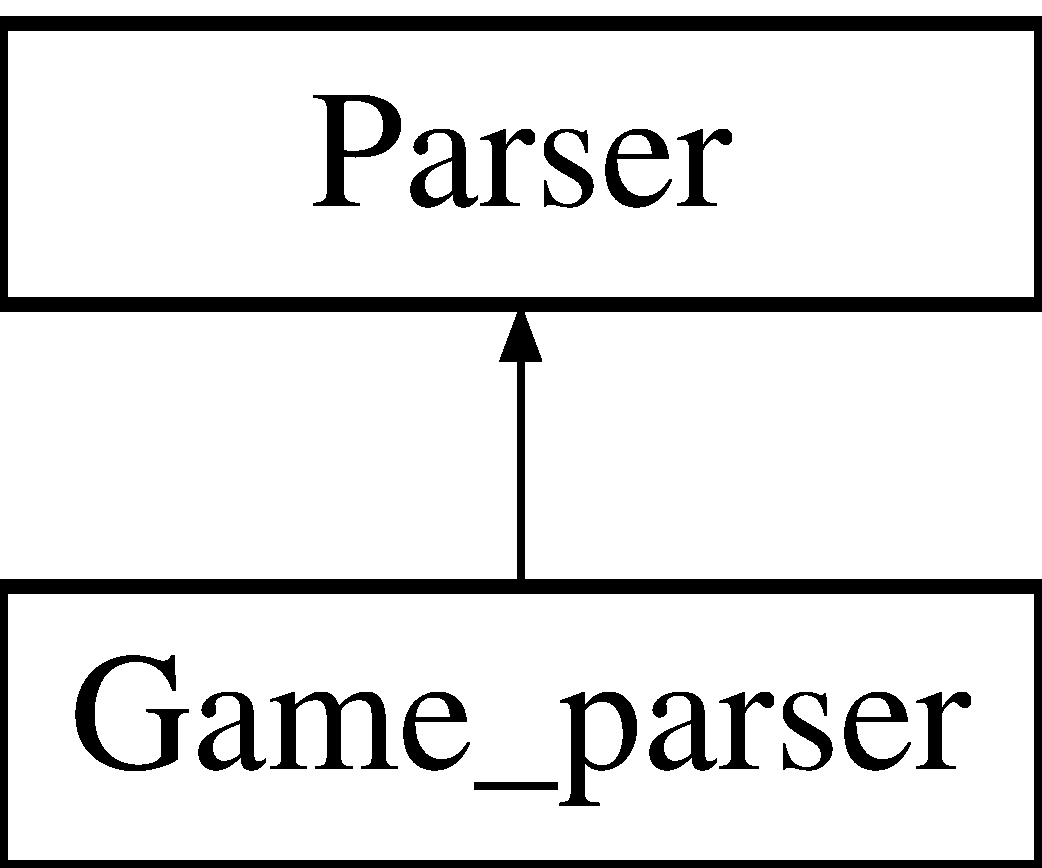
\includegraphics[height=2.000000cm]{class_game__parser}
\end{center}
\end{figure}
\subsection*{Public Member Functions}
\begin{DoxyCompactItemize}
\item 
\hyperlink{class_game__parser_ac871d4fd670b2b92c1ab27bbb2127e23}{Game\-\_\-parser} (std\-::ostream $\ast$stream, std\-::string \-\_\-board\-\_\-filename=\char`\"{}board\-\_\-file\-\_\-unspecified\char`\"{}, std\-::string \-\_\-actions\-\_\-filename=\char`\"{}moves\-\_\-file\-\_\-unspecified\char`\"{})
\item 
\hyperlink{class_game__parser_a2c346a615028b9cf26f7560620967a71}{Game\-\_\-parser} ()=default
\item 
\hyperlink{class_game}{Game} $\ast$ \hyperlink{class_game__parser_ad90be9cf48e0a2f99f7e526fab3fe33c}{parse\-\_\-game} (Ti\-Xml\-Element $\ast$board\-\_\-elem, Ti\-Xml\-Element $\ast$move\-\_\-elem=nullptr)
\end{DoxyCompactItemize}
\subsection*{Additional Inherited Members}


\subsection{Constructor \& Destructor Documentation}
\hypertarget{class_game__parser_ac871d4fd670b2b92c1ab27bbb2127e23}{\index{Game\-\_\-parser@{Game\-\_\-parser}!Game\-\_\-parser@{Game\-\_\-parser}}
\index{Game\-\_\-parser@{Game\-\_\-parser}!Game_parser@{Game\-\_\-parser}}
\subsubsection[{Game\-\_\-parser}]{\setlength{\rightskip}{0pt plus 5cm}Game\-\_\-parser\-::\-Game\-\_\-parser (
\begin{DoxyParamCaption}
\item[{std\-::ostream $\ast$}]{stream, }
\item[{std\-::string}]{\-\_\-board\-\_\-filename = {\ttfamily \char`\"{}board\-\_\-file\-\_\-unspecified\char`\"{}}, }
\item[{std\-::string}]{\-\_\-actions\-\_\-filename = {\ttfamily \char`\"{}moves\-\_\-file\-\_\-unspecified\char`\"{}}}
\end{DoxyParamCaption}
)}}\label{class_game__parser_ac871d4fd670b2b92c1ab27bbb2127e23}
\hypertarget{class_game__parser_a2c346a615028b9cf26f7560620967a71}{\index{Game\-\_\-parser@{Game\-\_\-parser}!Game\-\_\-parser@{Game\-\_\-parser}}
\index{Game\-\_\-parser@{Game\-\_\-parser}!Game_parser@{Game\-\_\-parser}}
\subsubsection[{Game\-\_\-parser}]{\setlength{\rightskip}{0pt plus 5cm}Game\-\_\-parser\-::\-Game\-\_\-parser (
\begin{DoxyParamCaption}
{}
\end{DoxyParamCaption}
)\hspace{0.3cm}{\ttfamily [default]}}}\label{class_game__parser_a2c346a615028b9cf26f7560620967a71}


\subsection{Member Function Documentation}
\hypertarget{class_game__parser_ad90be9cf48e0a2f99f7e526fab3fe33c}{\index{Game\-\_\-parser@{Game\-\_\-parser}!parse\-\_\-game@{parse\-\_\-game}}
\index{parse\-\_\-game@{parse\-\_\-game}!Game_parser@{Game\-\_\-parser}}
\subsubsection[{parse\-\_\-game}]{\setlength{\rightskip}{0pt plus 5cm}{\bf Game} $\ast$ Game\-\_\-parser\-::parse\-\_\-game (
\begin{DoxyParamCaption}
\item[{Ti\-Xml\-Element $\ast$}]{board\-\_\-elem, }
\item[{Ti\-Xml\-Element $\ast$}]{move\-\_\-elem = {\ttfamily nullptr}}
\end{DoxyParamCaption}
)}}\label{class_game__parser_ad90be9cf48e0a2f99f7e526fab3fe33c}


The documentation for this class was generated from the following files\-:\begin{DoxyCompactItemize}
\item 
parsers/\hyperlink{game__parser_8h}{game\-\_\-parser.\-h}\item 
parsers/\hyperlink{game__parser_8cpp}{game\-\_\-parser.\-cpp}\end{DoxyCompactItemize}

\hypertarget{class_gate}{\section{Gate Class Reference}
\label{class_gate}\index{Gate@{Gate}}
}


{\ttfamily \#include $<$gate.\-h$>$}

Inheritance diagram for Gate\-:\begin{figure}[H]
\begin{center}
\leavevmode
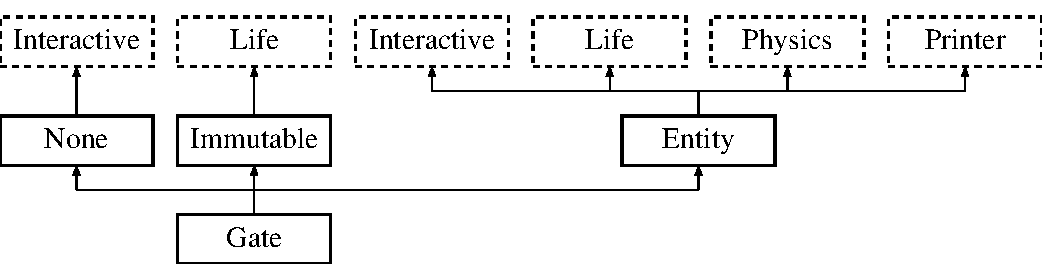
\includegraphics[height=3.000000cm]{class_gate}
\end{center}
\end{figure}
\subsection*{Public Member Functions}
\begin{DoxyCompactItemize}
\item 
\hyperlink{class_gate_a8c222415d9aa37b3057038e0fa1cb20f}{Gate} (unsigned int \hyperlink{class_entity_afa8f48eccdb09a290e2c1ded3f135363}{x}, unsigned \hyperlink{class_entity_a9d39843430829a89bb8233dbaadae4f1}{y}, std\-::string \-\_\-name)
\item 
int \hyperlink{class_gate_a92969268c88df32619ae44de87614cf8}{get\-\_\-height} ()
\item 
int \hyperlink{class_gate_a71358b21088e77ddcd7c1980e13ba063}{get\-\_\-weight} ()
\item 
char \hyperlink{class_gate_a4c957d7092b0c53a0a8e711142818dfa}{to\-\_\-char} ()
\item 
std\-::string \hyperlink{class_gate_a26fc1621b08010e7f712b68d665a6aa7}{get\-\_\-name} ()
\item 
void \hyperlink{class_gate_a6b6e01294cd8f5dbb5c93831c5cd3c3f}{open} ()
\item 
void \hyperlink{class_gate_a3733611cc86dfe641915fcbfaf4d41c8}{close} ()
\item 
void \hyperlink{class_gate_a194b57934f4ab3ed226a7c5fb45693bd}{info} (std\-::ostream \&out)
\item 
bool \hyperlink{class_gate_a5cb8530f286fcbe2c40d7f396176b805}{is\-\_\-open} ()
\end{DoxyCompactItemize}
\subsection*{Additional Inherited Members}


\subsection{Constructor \& Destructor Documentation}
\hypertarget{class_gate_a8c222415d9aa37b3057038e0fa1cb20f}{\index{Gate@{Gate}!Gate@{Gate}}
\index{Gate@{Gate}!Gate@{Gate}}
\subsubsection[{Gate}]{\setlength{\rightskip}{0pt plus 5cm}Gate\-::\-Gate (
\begin{DoxyParamCaption}
\item[{unsigned int}]{x, }
\item[{unsigned}]{y, }
\item[{std\-::string}]{\-\_\-name}
\end{DoxyParamCaption}
)}}\label{class_gate_a8c222415d9aa37b3057038e0fa1cb20f}


\subsection{Member Function Documentation}
\hypertarget{class_gate_a3733611cc86dfe641915fcbfaf4d41c8}{\index{Gate@{Gate}!close@{close}}
\index{close@{close}!Gate@{Gate}}
\subsubsection[{close}]{\setlength{\rightskip}{0pt plus 5cm}void Gate\-::close (
\begin{DoxyParamCaption}
{}
\end{DoxyParamCaption}
)}}\label{class_gate_a3733611cc86dfe641915fcbfaf4d41c8}
\hypertarget{class_gate_a92969268c88df32619ae44de87614cf8}{\index{Gate@{Gate}!get\-\_\-height@{get\-\_\-height}}
\index{get\-\_\-height@{get\-\_\-height}!Gate@{Gate}}
\subsubsection[{get\-\_\-height}]{\setlength{\rightskip}{0pt plus 5cm}int Gate\-::get\-\_\-height (
\begin{DoxyParamCaption}
{}
\end{DoxyParamCaption}
)\hspace{0.3cm}{\ttfamily [virtual]}}}\label{class_gate_a92969268c88df32619ae44de87614cf8}


Implements \hyperlink{class_physics_ae3e59e7723c9f0334b88baf60c01f376}{Physics}.

\hypertarget{class_gate_a26fc1621b08010e7f712b68d665a6aa7}{\index{Gate@{Gate}!get\-\_\-name@{get\-\_\-name}}
\index{get\-\_\-name@{get\-\_\-name}!Gate@{Gate}}
\subsubsection[{get\-\_\-name}]{\setlength{\rightskip}{0pt plus 5cm}std\-::string Gate\-::get\-\_\-name (
\begin{DoxyParamCaption}
{}
\end{DoxyParamCaption}
)}}\label{class_gate_a26fc1621b08010e7f712b68d665a6aa7}
\hypertarget{class_gate_a71358b21088e77ddcd7c1980e13ba063}{\index{Gate@{Gate}!get\-\_\-weight@{get\-\_\-weight}}
\index{get\-\_\-weight@{get\-\_\-weight}!Gate@{Gate}}
\subsubsection[{get\-\_\-weight}]{\setlength{\rightskip}{0pt plus 5cm}int Gate\-::get\-\_\-weight (
\begin{DoxyParamCaption}
{}
\end{DoxyParamCaption}
)\hspace{0.3cm}{\ttfamily [virtual]}}}\label{class_gate_a71358b21088e77ddcd7c1980e13ba063}


Implements \hyperlink{class_physics_a00580cf655d0569cc44f11b630cfcee7}{Physics}.

\hypertarget{class_gate_a194b57934f4ab3ed226a7c5fb45693bd}{\index{Gate@{Gate}!info@{info}}
\index{info@{info}!Gate@{Gate}}
\subsubsection[{info}]{\setlength{\rightskip}{0pt plus 5cm}void Gate\-::info (
\begin{DoxyParamCaption}
\item[{std\-::ostream \&}]{out}
\end{DoxyParamCaption}
)\hspace{0.3cm}{\ttfamily [virtual]}}}\label{class_gate_a194b57934f4ab3ed226a7c5fb45693bd}
Shows the info about the entity, used in the method \hyperlink{class_board_ae7e407126c1c113669e645a216fc7848}{Board\-::write\-\_\-board}. Is a pure virtual function for \hyperlink{class_entity}{Entity}. R\-E\-Q\-U\-I\-R\-E(\hyperlink{class_entity_af7f20142aa7883ca29a91c43e3511e48}{properly\-Initialized()}, \char`\"{}\-Entity wasn't initialized when calling info\char`\"{}) 

Implements \hyperlink{class_entity_aa694874d1f59971187de675d1e0c1fdf}{Entity}.

\hypertarget{class_gate_a5cb8530f286fcbe2c40d7f396176b805}{\index{Gate@{Gate}!is\-\_\-open@{is\-\_\-open}}
\index{is\-\_\-open@{is\-\_\-open}!Gate@{Gate}}
\subsubsection[{is\-\_\-open}]{\setlength{\rightskip}{0pt plus 5cm}bool Gate\-::is\-\_\-open (
\begin{DoxyParamCaption}
{}
\end{DoxyParamCaption}
)}}\label{class_gate_a5cb8530f286fcbe2c40d7f396176b805}
\hypertarget{class_gate_a6b6e01294cd8f5dbb5c93831c5cd3c3f}{\index{Gate@{Gate}!open@{open}}
\index{open@{open}!Gate@{Gate}}
\subsubsection[{open}]{\setlength{\rightskip}{0pt plus 5cm}void Gate\-::open (
\begin{DoxyParamCaption}
{}
\end{DoxyParamCaption}
)}}\label{class_gate_a6b6e01294cd8f5dbb5c93831c5cd3c3f}
\hypertarget{class_gate_a4c957d7092b0c53a0a8e711142818dfa}{\index{Gate@{Gate}!to\-\_\-char@{to\-\_\-char}}
\index{to\-\_\-char@{to\-\_\-char}!Gate@{Gate}}
\subsubsection[{to\-\_\-char}]{\setlength{\rightskip}{0pt plus 5cm}char Gate\-::to\-\_\-char (
\begin{DoxyParamCaption}
{}
\end{DoxyParamCaption}
)\hspace{0.3cm}{\ttfamily [virtual]}}}\label{class_gate_a4c957d7092b0c53a0a8e711142818dfa}


Implements \hyperlink{class_printer_a66ecfd99bb8bc0a88ed0fc1276c70e23}{Printer}.



The documentation for this class was generated from the following files\-:\begin{DoxyCompactItemize}
\item 
entities/\hyperlink{gate_8h}{gate.\-h}\item 
entities/\hyperlink{gate_8cpp}{gate.\-cpp}\end{DoxyCompactItemize}

\hypertarget{class_goal}{\section{Goal Class Reference}
\label{class_goal}\index{Goal@{Goal}}
}


{\ttfamily \#include $<$goal.\-h$>$}

Inheritance diagram for Goal\-:\begin{figure}[H]
\begin{center}
\leavevmode
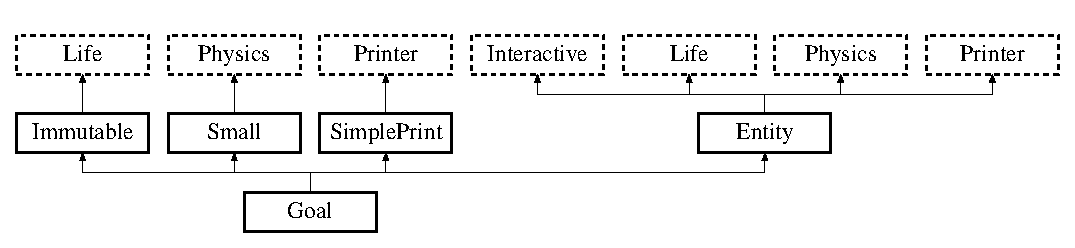
\includegraphics[height=2.891566cm]{class_goal}
\end{center}
\end{figure}
\subsection*{Public Member Functions}
\begin{DoxyCompactItemize}
\item 
\hyperlink{class_goal_aa06b63c82204ae51415a1c7dbfb36dfe}{Goal} (unsigned int \hyperlink{class_entity_afa8f48eccdb09a290e2c1ded3f135363}{x}, unsigned \hyperlink{class_entity_a9d39843430829a89bb8233dbaadae4f1}{y})
\item 
void \hyperlink{class_goal_adbce7419324f805e9b0527d85d033ce2}{info} (std\-::ostream \&out)
\end{DoxyCompactItemize}
\subsection*{Additional Inherited Members}


\subsection{Constructor \& Destructor Documentation}
\hypertarget{class_goal_aa06b63c82204ae51415a1c7dbfb36dfe}{\index{Goal@{Goal}!Goal@{Goal}}
\index{Goal@{Goal}!Goal@{Goal}}
\subsubsection[{Goal}]{\setlength{\rightskip}{0pt plus 5cm}Goal\-::\-Goal (
\begin{DoxyParamCaption}
\item[{unsigned int}]{x, }
\item[{unsigned}]{y}
\end{DoxyParamCaption}
)}}\label{class_goal_aa06b63c82204ae51415a1c7dbfb36dfe}
E\-N\-S\-U\-R\-E(\hyperlink{class_entity_af7f20142aa7883ca29a91c43e3511e48}{properly\-Initialized()}, \char`\"{}\-Constructor must end...\char`\"{}) 

\subsection{Member Function Documentation}
\hypertarget{class_goal_adbce7419324f805e9b0527d85d033ce2}{\index{Goal@{Goal}!info@{info}}
\index{info@{info}!Goal@{Goal}}
\subsubsection[{info}]{\setlength{\rightskip}{0pt plus 5cm}void Goal\-::info (
\begin{DoxyParamCaption}
\item[{std\-::ostream \&}]{out}
\end{DoxyParamCaption}
)\hspace{0.3cm}{\ttfamily [virtual]}}}\label{class_goal_adbce7419324f805e9b0527d85d033ce2}
R\-E\-Q\-U\-I\-R\-E(\hyperlink{class_entity_af7f20142aa7883ca29a91c43e3511e48}{properly\-Initialized()}, \char`\"{}\-Goal wasn't initialized when calling info\char`\"{}) 

Implements \hyperlink{class_entity_aa694874d1f59971187de675d1e0c1fdf}{Entity}.



The documentation for this class was generated from the following files\-:\begin{DoxyCompactItemize}
\item 
entities/\hyperlink{goal_8h}{goal.\-h}\item 
entities/\hyperlink{goal_8cpp}{goal.\-cpp}\end{DoxyCompactItemize}

\hypertarget{class_handler}{\section{Handler Class Reference}
\label{class_handler}\index{Handler@{Handler}}
}


{\ttfamily \#include $<$handler.\-h$>$}

Inheritance diagram for Handler\-:\begin{figure}[H]
\begin{center}
\leavevmode
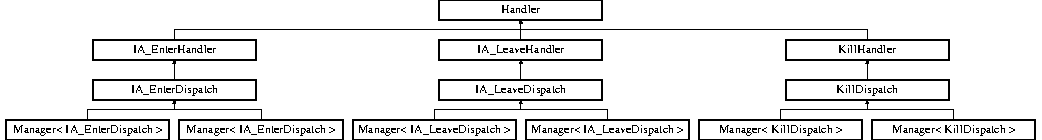
\includegraphics[height=1.885522cm]{class_handler}
\end{center}
\end{figure}
\subsection*{Public Member Functions}
\begin{DoxyCompactItemize}
\item 
\hyperlink{class_handler_a34e86cc5a32e5fe9b4675f16f7b77383}{Handler} (\hyperlink{class_game}{Game} $\ast$\-\_\-g)
\item 
\hyperlink{class_handler_a6eb353aae22778422bc71f6b00aad8be}{Handler} ()
\item 
void \hyperlink{class_handler_ac0ff81e19943c7c1c360dd5597e5b658}{set\-Game} (\hyperlink{class_game}{Game} $\ast$\-\_\-g)
\end{DoxyCompactItemize}
\subsection*{Protected Attributes}
\begin{DoxyCompactItemize}
\item 
\hyperlink{class_game}{Game} $\ast$ \hyperlink{class_handler_a1f0fad79bbada9ca4f5fd3e649a19808}{game}
\end{DoxyCompactItemize}


\subsection{Constructor \& Destructor Documentation}
\hypertarget{class_handler_a34e86cc5a32e5fe9b4675f16f7b77383}{\index{Handler@{Handler}!Handler@{Handler}}
\index{Handler@{Handler}!Handler@{Handler}}
\subsubsection[{Handler}]{\setlength{\rightskip}{0pt plus 5cm}Handler\-::\-Handler (
\begin{DoxyParamCaption}
\item[{{\bf Game} $\ast$}]{\-\_\-g}
\end{DoxyParamCaption}
)}}\label{class_handler_a34e86cc5a32e5fe9b4675f16f7b77383}
\hypertarget{class_handler_a6eb353aae22778422bc71f6b00aad8be}{\index{Handler@{Handler}!Handler@{Handler}}
\index{Handler@{Handler}!Handler@{Handler}}
\subsubsection[{Handler}]{\setlength{\rightskip}{0pt plus 5cm}Handler\-::\-Handler (
\begin{DoxyParamCaption}
{}
\end{DoxyParamCaption}
)}}\label{class_handler_a6eb353aae22778422bc71f6b00aad8be}


\subsection{Member Function Documentation}
\hypertarget{class_handler_ac0ff81e19943c7c1c360dd5597e5b658}{\index{Handler@{Handler}!set\-Game@{set\-Game}}
\index{set\-Game@{set\-Game}!Handler@{Handler}}
\subsubsection[{set\-Game}]{\setlength{\rightskip}{0pt plus 5cm}void Handler\-::set\-Game (
\begin{DoxyParamCaption}
\item[{{\bf Game} $\ast$}]{\-\_\-g}
\end{DoxyParamCaption}
)}}\label{class_handler_ac0ff81e19943c7c1c360dd5597e5b658}


\subsection{Member Data Documentation}
\hypertarget{class_handler_a1f0fad79bbada9ca4f5fd3e649a19808}{\index{Handler@{Handler}!game@{game}}
\index{game@{game}!Handler@{Handler}}
\subsubsection[{game}]{\setlength{\rightskip}{0pt plus 5cm}{\bf Game}$\ast$ Handler\-::game\hspace{0.3cm}{\ttfamily [protected]}}}\label{class_handler_a1f0fad79bbada9ca4f5fd3e649a19808}


The documentation for this class was generated from the following files\-:\begin{DoxyCompactItemize}
\item 
events/\hyperlink{handler_8h}{handler.\-h}\item 
events/\hyperlink{handler_8cpp}{handler.\-cpp}\end{DoxyCompactItemize}

\hypertarget{class_i_a___enter_dispatch}{\section{I\-A\-\_\-\-Enter\-Dispatch Class Reference}
\label{class_i_a___enter_dispatch}\index{I\-A\-\_\-\-Enter\-Dispatch@{I\-A\-\_\-\-Enter\-Dispatch}}
}


{\ttfamily \#include $<$dispatchers.\-h$>$}

Inheritance diagram for I\-A\-\_\-\-Enter\-Dispatch\-:\begin{figure}[H]
\begin{center}
\leavevmode
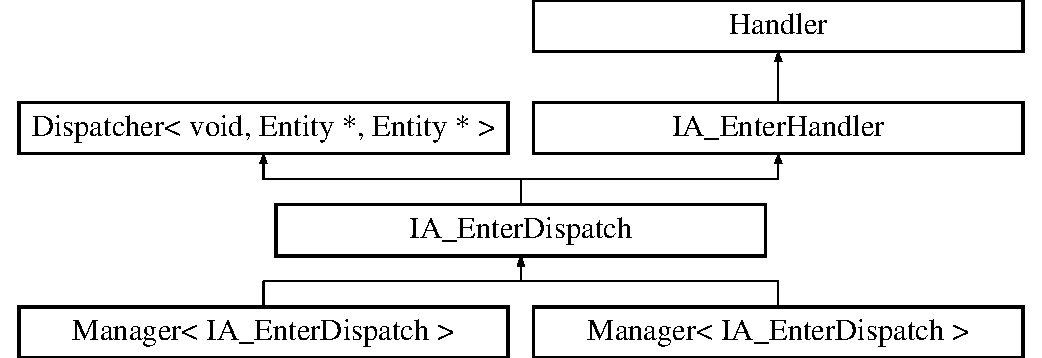
\includegraphics[height=4.000000cm]{class_i_a___enter_dispatch}
\end{center}
\end{figure}
\subsection*{Public Member Functions}
\begin{DoxyCompactItemize}
\item 
int \hyperlink{class_i_a___enter_dispatch_a88d924c856eb8afde208c45feb19eaed}{get\-Rule} (\hyperlink{class_entity}{Entity} $\ast$\-\_\-\-\_\-\-Entity0, \hyperlink{class_entity}{Entity} $\ast$\-\_\-\-\_\-\-Entity1)
\item 
void \hyperlink{class_i_a___enter_dispatch_af5e262ccfebfbea6fb0b3167b77c2d6c}{do\-Rule} (int rulenum, \hyperlink{class_entity}{Entity} $\ast$\-\_\-\-\_\-\-Entity0, \hyperlink{class_entity}{Entity} $\ast$\-\_\-\-\_\-\-Entity1)
\end{DoxyCompactItemize}
\subsection*{Additional Inherited Members}


\subsection{Member Function Documentation}
\hypertarget{class_i_a___enter_dispatch_af5e262ccfebfbea6fb0b3167b77c2d6c}{\index{I\-A\-\_\-\-Enter\-Dispatch@{I\-A\-\_\-\-Enter\-Dispatch}!do\-Rule@{do\-Rule}}
\index{do\-Rule@{do\-Rule}!IA_EnterDispatch@{I\-A\-\_\-\-Enter\-Dispatch}}
\subsubsection[{do\-Rule}]{\setlength{\rightskip}{0pt plus 5cm}void I\-A\-\_\-\-Enter\-Dispatch\-::do\-Rule (
\begin{DoxyParamCaption}
\item[{int}]{rulenum, }
\item[{{\bf Entity} $\ast$}]{\-\_\-\-\_\-\-Entity0, }
\item[{{\bf Entity} $\ast$}]{\-\_\-\-\_\-\-Entity1}
\end{DoxyParamCaption}
)}}\label{class_i_a___enter_dispatch_af5e262ccfebfbea6fb0b3167b77c2d6c}
\hypertarget{class_i_a___enter_dispatch_a88d924c856eb8afde208c45feb19eaed}{\index{I\-A\-\_\-\-Enter\-Dispatch@{I\-A\-\_\-\-Enter\-Dispatch}!get\-Rule@{get\-Rule}}
\index{get\-Rule@{get\-Rule}!IA_EnterDispatch@{I\-A\-\_\-\-Enter\-Dispatch}}
\subsubsection[{get\-Rule}]{\setlength{\rightskip}{0pt plus 5cm}int I\-A\-\_\-\-Enter\-Dispatch\-::get\-Rule (
\begin{DoxyParamCaption}
\item[{{\bf Entity} $\ast$}]{\-\_\-\-\_\-\-Entity0, }
\item[{{\bf Entity} $\ast$}]{\-\_\-\-\_\-\-Entity1}
\end{DoxyParamCaption}
)}}\label{class_i_a___enter_dispatch_a88d924c856eb8afde208c45feb19eaed}


The documentation for this class was generated from the following files\-:\begin{DoxyCompactItemize}
\item 
events/dispatch/\hyperlink{dispatchers_8h}{dispatchers.\-h}\item 
events/dispatch/\hyperlink{dispatchers_8cpp}{dispatchers.\-cpp}\end{DoxyCompactItemize}

\hypertarget{class_i_a___enter_handler}{\section{I\-A\-\_\-\-Enter\-Handler Class Reference}
\label{class_i_a___enter_handler}\index{I\-A\-\_\-\-Enter\-Handler@{I\-A\-\_\-\-Enter\-Handler}}
}


{\ttfamily \#include $<$ia\-\_\-enterhandler.\-h$>$}

Inheritance diagram for I\-A\-\_\-\-Enter\-Handler\-:\begin{figure}[H]
\begin{center}
\leavevmode
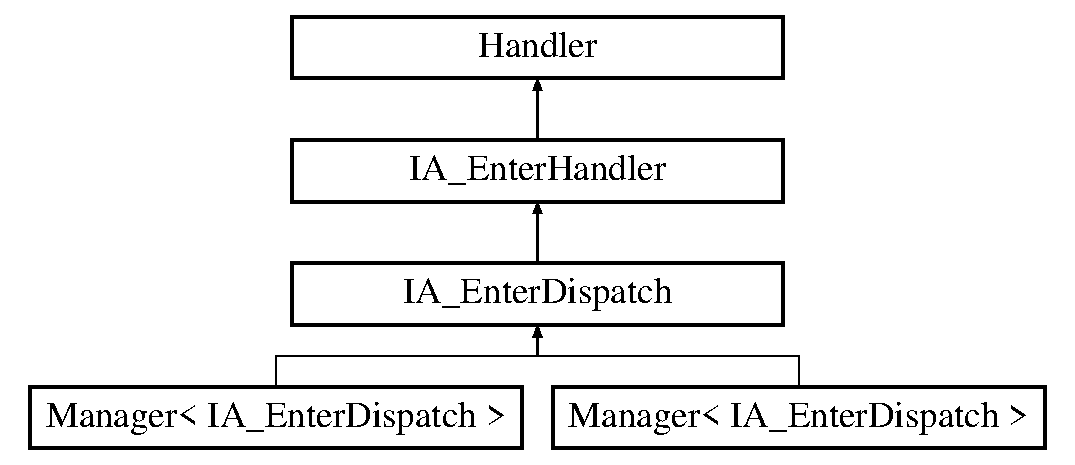
\includegraphics[height=4.000000cm]{class_i_a___enter_handler}
\end{center}
\end{figure}
\subsection*{Public Member Functions}
\begin{DoxyCompactItemize}
\item 
void \hyperlink{class_i_a___enter_handler_a1eed327c0520e3e5352952be8db4e407}{on\-Enter} (\hyperlink{class_player}{Player} $\ast$p, \hyperlink{class_goal}{Goal} $\ast$g)
\item 
void \hyperlink{class_i_a___enter_handler_a49564d959017c61f4afbbfea7c5c3eeb}{on\-Enter} (\hyperlink{class_actor}{Actor} $\ast$a, \hyperlink{class_boobytrap}{Boobytrap} $\ast$b)
\item 
void \hyperlink{class_i_a___enter_handler_a340a0096594990ce52886393b98387b6}{on\-Enter} (\hyperlink{class_entity}{Entity} $\ast$e, \hyperlink{class_button}{Button} $\ast$b)
\item 
void \hyperlink{class_i_a___enter_handler_a42dd4db9a499f32fc3be9ae956e829c8}{on\-Enter} (\hyperlink{class_entity}{Entity} $\ast$e, \hyperlink{class_entity}{Entity} $\ast$f)
\end{DoxyCompactItemize}
\subsection*{Additional Inherited Members}


\subsection{Member Function Documentation}
\hypertarget{class_i_a___enter_handler_a1eed327c0520e3e5352952be8db4e407}{\index{I\-A\-\_\-\-Enter\-Handler@{I\-A\-\_\-\-Enter\-Handler}!on\-Enter@{on\-Enter}}
\index{on\-Enter@{on\-Enter}!IA_EnterHandler@{I\-A\-\_\-\-Enter\-Handler}}
\subsubsection[{on\-Enter}]{\setlength{\rightskip}{0pt plus 5cm}void I\-A\-\_\-\-Enter\-Handler\-::on\-Enter (
\begin{DoxyParamCaption}
\item[{{\bf Player} $\ast$}]{p, }
\item[{{\bf Goal} $\ast$}]{g}
\end{DoxyParamCaption}
)}}\label{class_i_a___enter_handler_a1eed327c0520e3e5352952be8db4e407}
\hypertarget{class_i_a___enter_handler_a49564d959017c61f4afbbfea7c5c3eeb}{\index{I\-A\-\_\-\-Enter\-Handler@{I\-A\-\_\-\-Enter\-Handler}!on\-Enter@{on\-Enter}}
\index{on\-Enter@{on\-Enter}!IA_EnterHandler@{I\-A\-\_\-\-Enter\-Handler}}
\subsubsection[{on\-Enter}]{\setlength{\rightskip}{0pt plus 5cm}void I\-A\-\_\-\-Enter\-Handler\-::on\-Enter (
\begin{DoxyParamCaption}
\item[{{\bf Actor} $\ast$}]{a, }
\item[{{\bf Boobytrap} $\ast$}]{b}
\end{DoxyParamCaption}
)}}\label{class_i_a___enter_handler_a49564d959017c61f4afbbfea7c5c3eeb}
\hypertarget{class_i_a___enter_handler_a340a0096594990ce52886393b98387b6}{\index{I\-A\-\_\-\-Enter\-Handler@{I\-A\-\_\-\-Enter\-Handler}!on\-Enter@{on\-Enter}}
\index{on\-Enter@{on\-Enter}!IA_EnterHandler@{I\-A\-\_\-\-Enter\-Handler}}
\subsubsection[{on\-Enter}]{\setlength{\rightskip}{0pt plus 5cm}void I\-A\-\_\-\-Enter\-Handler\-::on\-Enter (
\begin{DoxyParamCaption}
\item[{{\bf Entity} $\ast$}]{e, }
\item[{{\bf Button} $\ast$}]{b}
\end{DoxyParamCaption}
)}}\label{class_i_a___enter_handler_a340a0096594990ce52886393b98387b6}
\hypertarget{class_i_a___enter_handler_a42dd4db9a499f32fc3be9ae956e829c8}{\index{I\-A\-\_\-\-Enter\-Handler@{I\-A\-\_\-\-Enter\-Handler}!on\-Enter@{on\-Enter}}
\index{on\-Enter@{on\-Enter}!IA_EnterHandler@{I\-A\-\_\-\-Enter\-Handler}}
\subsubsection[{on\-Enter}]{\setlength{\rightskip}{0pt plus 5cm}void I\-A\-\_\-\-Enter\-Handler\-::on\-Enter (
\begin{DoxyParamCaption}
\item[{{\bf Entity} $\ast$}]{e, }
\item[{{\bf Entity} $\ast$}]{f}
\end{DoxyParamCaption}
)}}\label{class_i_a___enter_handler_a42dd4db9a499f32fc3be9ae956e829c8}


The documentation for this class was generated from the following files\-:\begin{DoxyCompactItemize}
\item 
events/\hyperlink{ia__enterhandler_8h}{ia\-\_\-enterhandler.\-h}\item 
events/\hyperlink{ia__enterhandler_8cpp}{ia\-\_\-enterhandler.\-cpp}\end{DoxyCompactItemize}

\hypertarget{class_i_a___leave_dispatch}{\section{I\-A\-\_\-\-Leave\-Dispatch Class Reference}
\label{class_i_a___leave_dispatch}\index{I\-A\-\_\-\-Leave\-Dispatch@{I\-A\-\_\-\-Leave\-Dispatch}}
}


{\ttfamily \#include $<$dispatchers.\-h$>$}

Inheritance diagram for I\-A\-\_\-\-Leave\-Dispatch\-:\begin{figure}[H]
\begin{center}
\leavevmode
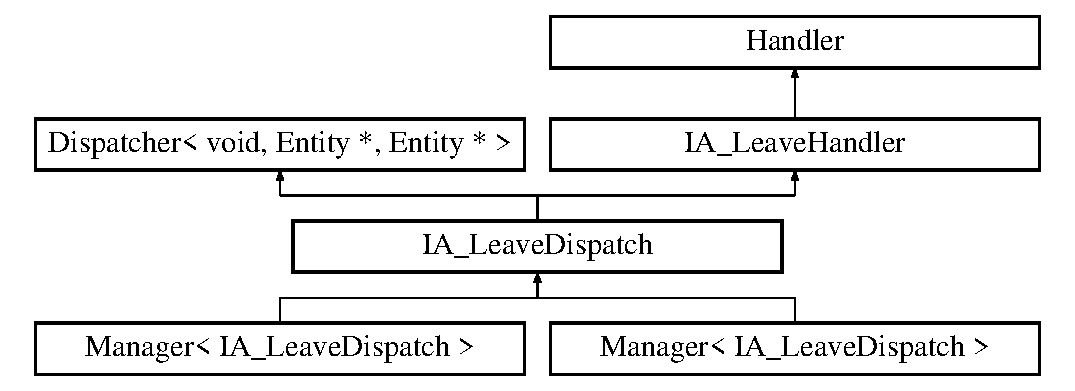
\includegraphics[height=4.000000cm]{class_i_a___leave_dispatch}
\end{center}
\end{figure}
\subsection*{Public Member Functions}
\begin{DoxyCompactItemize}
\item 
int \hyperlink{class_i_a___leave_dispatch_a41be1f81e47a0fd1a67315165f2bbb89}{get\-Rule} (\hyperlink{class_entity}{Entity} $\ast$\-\_\-\-\_\-\-Entity0, \hyperlink{class_entity}{Entity} $\ast$\-\_\-\-\_\-\-Entity1)
\item 
void \hyperlink{class_i_a___leave_dispatch_a13f472a72cc1db91fc994a9b2aba7b9a}{do\-Rule} (int rulenum, \hyperlink{class_entity}{Entity} $\ast$\-\_\-\-\_\-\-Entity0, \hyperlink{class_entity}{Entity} $\ast$\-\_\-\-\_\-\-Entity1)
\end{DoxyCompactItemize}
\subsection*{Additional Inherited Members}


\subsection{Member Function Documentation}
\hypertarget{class_i_a___leave_dispatch_a13f472a72cc1db91fc994a9b2aba7b9a}{\index{I\-A\-\_\-\-Leave\-Dispatch@{I\-A\-\_\-\-Leave\-Dispatch}!do\-Rule@{do\-Rule}}
\index{do\-Rule@{do\-Rule}!IA_LeaveDispatch@{I\-A\-\_\-\-Leave\-Dispatch}}
\subsubsection[{do\-Rule}]{\setlength{\rightskip}{0pt plus 5cm}void I\-A\-\_\-\-Leave\-Dispatch\-::do\-Rule (
\begin{DoxyParamCaption}
\item[{int}]{rulenum, }
\item[{{\bf Entity} $\ast$}]{\-\_\-\-\_\-\-Entity0, }
\item[{{\bf Entity} $\ast$}]{\-\_\-\-\_\-\-Entity1}
\end{DoxyParamCaption}
)}}\label{class_i_a___leave_dispatch_a13f472a72cc1db91fc994a9b2aba7b9a}
\hypertarget{class_i_a___leave_dispatch_a41be1f81e47a0fd1a67315165f2bbb89}{\index{I\-A\-\_\-\-Leave\-Dispatch@{I\-A\-\_\-\-Leave\-Dispatch}!get\-Rule@{get\-Rule}}
\index{get\-Rule@{get\-Rule}!IA_LeaveDispatch@{I\-A\-\_\-\-Leave\-Dispatch}}
\subsubsection[{get\-Rule}]{\setlength{\rightskip}{0pt plus 5cm}int I\-A\-\_\-\-Leave\-Dispatch\-::get\-Rule (
\begin{DoxyParamCaption}
\item[{{\bf Entity} $\ast$}]{\-\_\-\-\_\-\-Entity0, }
\item[{{\bf Entity} $\ast$}]{\-\_\-\-\_\-\-Entity1}
\end{DoxyParamCaption}
)}}\label{class_i_a___leave_dispatch_a41be1f81e47a0fd1a67315165f2bbb89}


The documentation for this class was generated from the following files\-:\begin{DoxyCompactItemize}
\item 
events/dispatch/\hyperlink{dispatchers_8h}{dispatchers.\-h}\item 
events/dispatch/\hyperlink{dispatchers_8cpp}{dispatchers.\-cpp}\end{DoxyCompactItemize}

\hypertarget{class_i_a___leave_handler}{\section{I\-A\-\_\-\-Leave\-Handler Class Reference}
\label{class_i_a___leave_handler}\index{I\-A\-\_\-\-Leave\-Handler@{I\-A\-\_\-\-Leave\-Handler}}
}


{\ttfamily \#include $<$ia\-\_\-leavehandler.\-h$>$}

Inheritance diagram for I\-A\-\_\-\-Leave\-Handler\-:\begin{figure}[H]
\begin{center}
\leavevmode
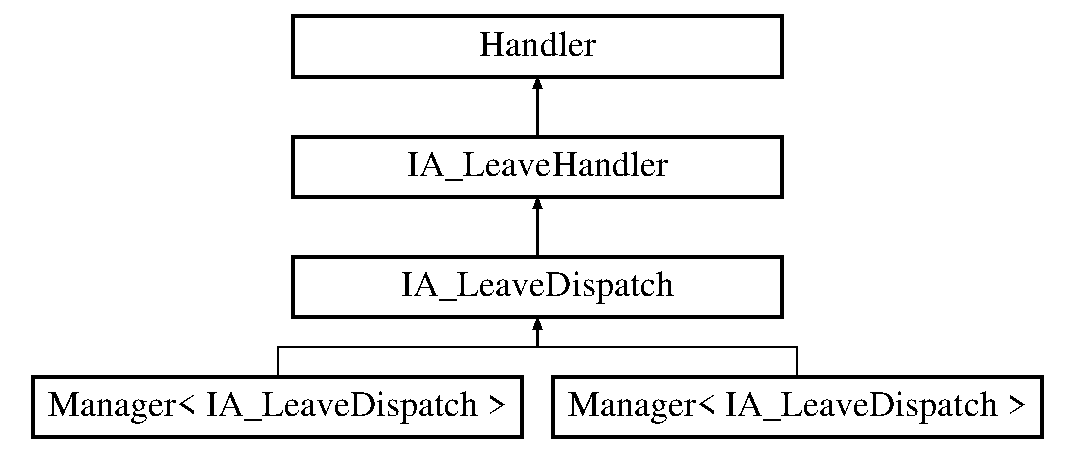
\includegraphics[height=4.000000cm]{class_i_a___leave_handler}
\end{center}
\end{figure}
\subsection*{Public Member Functions}
\begin{DoxyCompactItemize}
\item 
void \hyperlink{class_i_a___leave_handler_a5f4f139c55b4a4938c15eaff18bf870c}{on\-Leave} (\hyperlink{class_entity}{Entity} $\ast$e, \hyperlink{class_button}{Button} $\ast$b)
\item 
void \hyperlink{class_i_a___leave_handler_a40f4d48eb0b7fd01a3c663cb6fbfb871}{on\-Leave} (\hyperlink{class_entity}{Entity} $\ast$e, \hyperlink{class_entity}{Entity} $\ast$f)
\end{DoxyCompactItemize}
\subsection*{Additional Inherited Members}


\subsection{Member Function Documentation}
\hypertarget{class_i_a___leave_handler_a5f4f139c55b4a4938c15eaff18bf870c}{\index{I\-A\-\_\-\-Leave\-Handler@{I\-A\-\_\-\-Leave\-Handler}!on\-Leave@{on\-Leave}}
\index{on\-Leave@{on\-Leave}!IA_LeaveHandler@{I\-A\-\_\-\-Leave\-Handler}}
\subsubsection[{on\-Leave}]{\setlength{\rightskip}{0pt plus 5cm}void I\-A\-\_\-\-Leave\-Handler\-::on\-Leave (
\begin{DoxyParamCaption}
\item[{{\bf Entity} $\ast$}]{e, }
\item[{{\bf Button} $\ast$}]{b}
\end{DoxyParamCaption}
)}}\label{class_i_a___leave_handler_a5f4f139c55b4a4938c15eaff18bf870c}
\hypertarget{class_i_a___leave_handler_a40f4d48eb0b7fd01a3c663cb6fbfb871}{\index{I\-A\-\_\-\-Leave\-Handler@{I\-A\-\_\-\-Leave\-Handler}!on\-Leave@{on\-Leave}}
\index{on\-Leave@{on\-Leave}!IA_LeaveHandler@{I\-A\-\_\-\-Leave\-Handler}}
\subsubsection[{on\-Leave}]{\setlength{\rightskip}{0pt plus 5cm}void I\-A\-\_\-\-Leave\-Handler\-::on\-Leave (
\begin{DoxyParamCaption}
\item[{{\bf Entity} $\ast$}]{e, }
\item[{{\bf Entity} $\ast$}]{f}
\end{DoxyParamCaption}
)}}\label{class_i_a___leave_handler_a40f4d48eb0b7fd01a3c663cb6fbfb871}


The documentation for this class was generated from the following files\-:\begin{DoxyCompactItemize}
\item 
events/\hyperlink{ia__leavehandler_8h}{ia\-\_\-leavehandler.\-h}\item 
events/\hyperlink{ia__leavehandler_8cpp}{ia\-\_\-leavehandler.\-cpp}\end{DoxyCompactItemize}

\hypertarget{class_immutable}{\section{Immutable Class Reference}
\label{class_immutable}\index{Immutable@{Immutable}}
}


{\ttfamily \#include $<$immutable.\-h$>$}

Inheritance diagram for Immutable\-:\begin{figure}[H]
\begin{center}
\leavevmode
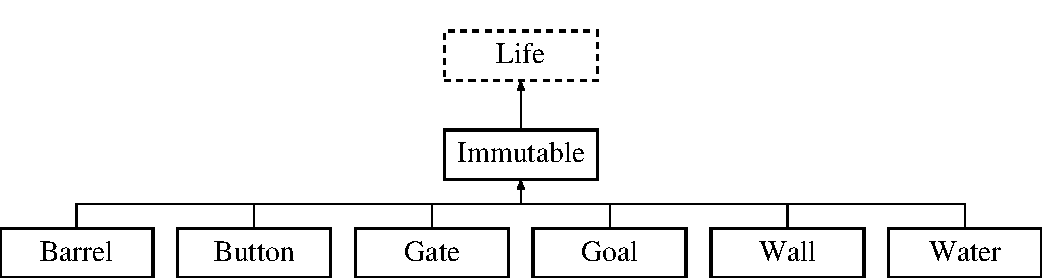
\includegraphics[height=3.000000cm]{class_immutable}
\end{center}
\end{figure}
\subsection*{Public Member Functions}
\begin{DoxyCompactItemize}
\item 
bool \hyperlink{class_immutable_a0460b0dffb45031b03bb1835a86c3185}{is\-\_\-alive} ()
\item 
void \hyperlink{class_immutable_ad74ffebf832d588e19e3746c09c90d1a}{kill} ()
\end{DoxyCompactItemize}


\subsection{Member Function Documentation}
\hypertarget{class_immutable_a0460b0dffb45031b03bb1835a86c3185}{\index{Immutable@{Immutable}!is\-\_\-alive@{is\-\_\-alive}}
\index{is\-\_\-alive@{is\-\_\-alive}!Immutable@{Immutable}}
\subsubsection[{is\-\_\-alive}]{\setlength{\rightskip}{0pt plus 5cm}bool Immutable\-::is\-\_\-alive (
\begin{DoxyParamCaption}
{}
\end{DoxyParamCaption}
)\hspace{0.3cm}{\ttfamily [virtual]}}}\label{class_immutable_a0460b0dffb45031b03bb1835a86c3185}


Implements \hyperlink{class_life_a8f79fb2cb57ef2a76e0c0feba345c68c}{Life}.

\hypertarget{class_immutable_ad74ffebf832d588e19e3746c09c90d1a}{\index{Immutable@{Immutable}!kill@{kill}}
\index{kill@{kill}!Immutable@{Immutable}}
\subsubsection[{kill}]{\setlength{\rightskip}{0pt plus 5cm}void Immutable\-::kill (
\begin{DoxyParamCaption}
{}
\end{DoxyParamCaption}
)\hspace{0.3cm}{\ttfamily [virtual]}}}\label{class_immutable_ad74ffebf832d588e19e3746c09c90d1a}


Implements \hyperlink{class_life_a40b24b079b08e3a80a582eff6be8faa3}{Life}.



The documentation for this class was generated from the following files\-:\begin{DoxyCompactItemize}
\item 
entities/life/\hyperlink{immutable_8h}{immutable.\-h}\item 
entities/life/\hyperlink{immutable_8cpp}{immutable.\-cpp}\end{DoxyCompactItemize}

\hypertarget{class_interactive}{\section{Interactive Class Reference}
\label{class_interactive}\index{Interactive@{Interactive}}
}


{\ttfamily \#include $<$ia.\-h$>$}

Inheritance diagram for Interactive\-:\begin{figure}[H]
\begin{center}
\leavevmode
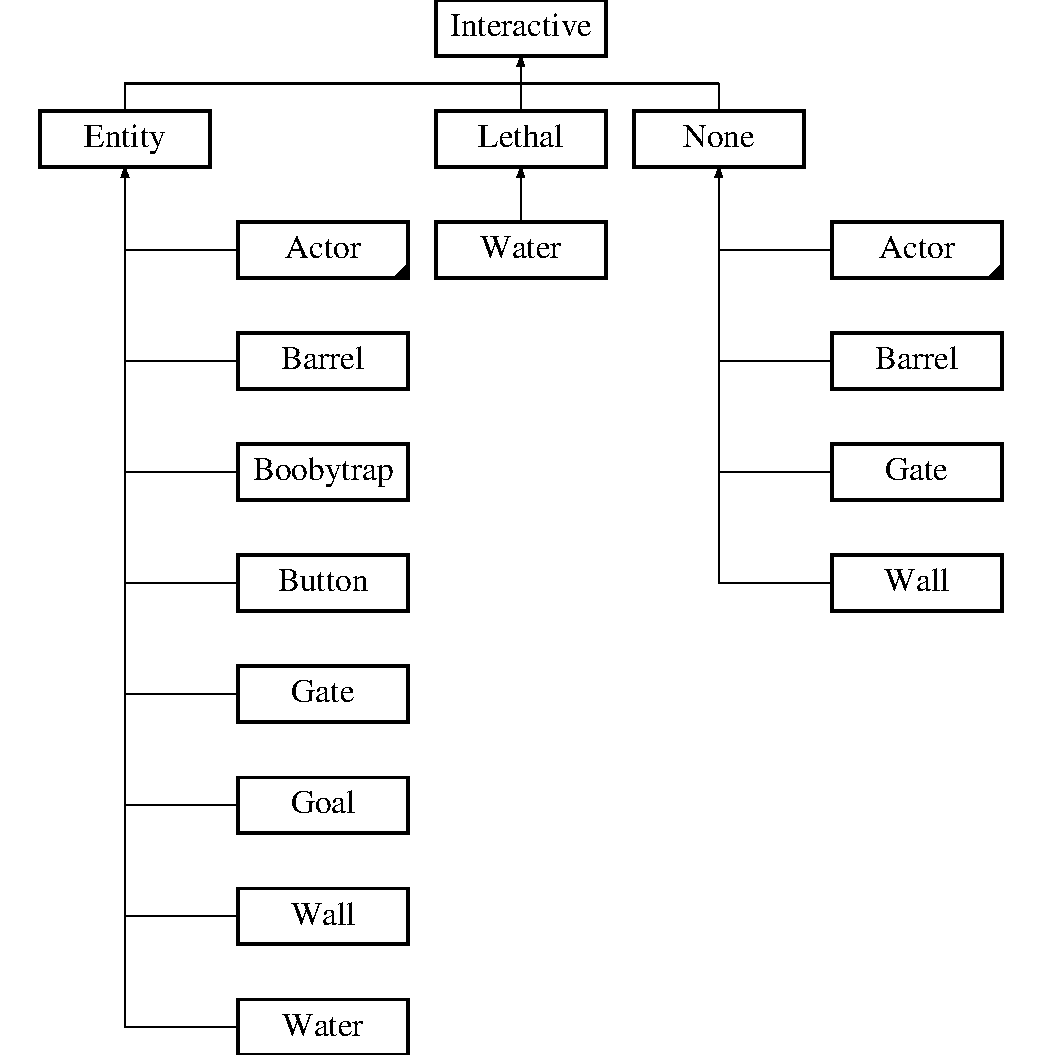
\includegraphics[height=10.000000cm]{class_interactive}
\end{center}
\end{figure}
\subsection*{Public Member Functions}
\begin{DoxyCompactItemize}
\item 
virtual void \hyperlink{class_interactive_a07537d2f82f4b05daaa9abfe24e16673}{\-\_\-\-\_\-polymorphic\-\_\-\-\_\-} ()
\item 
virtual \hyperlink{class_interactive_a2da1a8373dcd149b8b43c29c155e15a8}{$\sim$\-Interactive} ()
\end{DoxyCompactItemize}


\subsection{Constructor \& Destructor Documentation}
\hypertarget{class_interactive_a2da1a8373dcd149b8b43c29c155e15a8}{\index{Interactive@{Interactive}!$\sim$\-Interactive@{$\sim$\-Interactive}}
\index{$\sim$\-Interactive@{$\sim$\-Interactive}!Interactive@{Interactive}}
\subsubsection[{$\sim$\-Interactive}]{\setlength{\rightskip}{0pt plus 5cm}virtual Interactive\-::$\sim$\-Interactive (
\begin{DoxyParamCaption}
{}
\end{DoxyParamCaption}
)\hspace{0.3cm}{\ttfamily [inline]}, {\ttfamily [virtual]}}}\label{class_interactive_a2da1a8373dcd149b8b43c29c155e15a8}


\subsection{Member Function Documentation}
\hypertarget{class_interactive_a07537d2f82f4b05daaa9abfe24e16673}{\index{Interactive@{Interactive}!\-\_\-\-\_\-polymorphic\-\_\-\-\_\-@{\-\_\-\-\_\-polymorphic\-\_\-\-\_\-}}
\index{\-\_\-\-\_\-polymorphic\-\_\-\-\_\-@{\-\_\-\-\_\-polymorphic\-\_\-\-\_\-}!Interactive@{Interactive}}
\subsubsection[{\-\_\-\-\_\-polymorphic\-\_\-\-\_\-}]{\setlength{\rightskip}{0pt plus 5cm}virtual void Interactive\-::\-\_\-\-\_\-polymorphic\-\_\-\-\_\- (
\begin{DoxyParamCaption}
{}
\end{DoxyParamCaption}
)\hspace{0.3cm}{\ttfamily [inline]}, {\ttfamily [virtual]}}}\label{class_interactive_a07537d2f82f4b05daaa9abfe24e16673}


Reimplemented in \hyperlink{class_entity_a11d5655c6e057fb86551402380009c01}{Entity}.



The documentation for this class was generated from the following file\-:\begin{DoxyCompactItemize}
\item 
entities/ia/\hyperlink{ia_8h}{ia.\-h}\end{DoxyCompactItemize}

\hypertarget{class_kill_dispatch}{\section{Kill\-Dispatch Class Reference}
\label{class_kill_dispatch}\index{Kill\-Dispatch@{Kill\-Dispatch}}
}


{\ttfamily \#include $<$dispatchers.\-h$>$}

Inheritance diagram for Kill\-Dispatch\-:\begin{figure}[H]
\begin{center}
\leavevmode
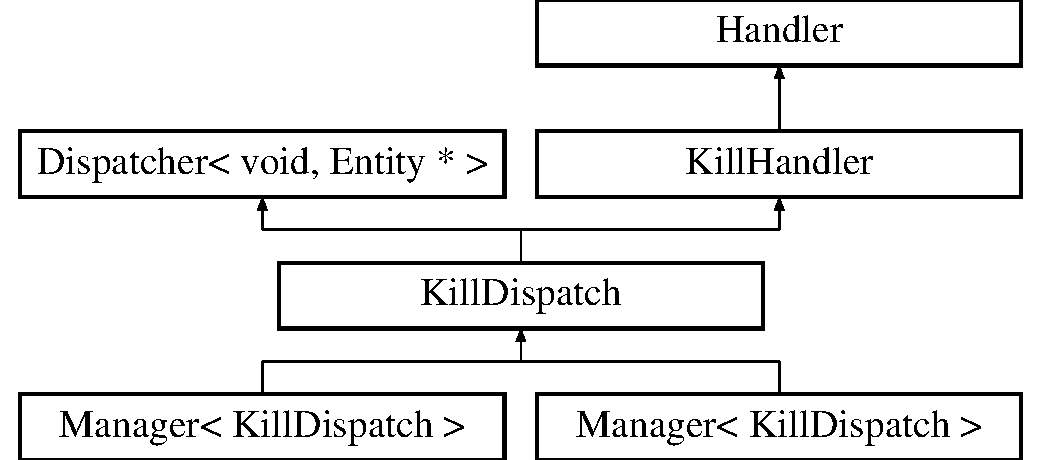
\includegraphics[height=4.000000cm]{class_kill_dispatch}
\end{center}
\end{figure}
\subsection*{Public Member Functions}
\begin{DoxyCompactItemize}
\item 
int \hyperlink{class_kill_dispatch_a3dabfd881b5b70d04048469f6161e8b2}{get\-Rule} (\hyperlink{class_entity}{Entity} $\ast$\-\_\-\-\_\-\-Entity0)
\item 
void \hyperlink{class_kill_dispatch_a77dc8cd9a45c9753fe2efdbd1080e721}{do\-Rule} (int rulenum, \hyperlink{class_entity}{Entity} $\ast$\-\_\-\-\_\-\-Entity0)
\end{DoxyCompactItemize}
\subsection*{Additional Inherited Members}


\subsection{Member Function Documentation}
\hypertarget{class_kill_dispatch_a77dc8cd9a45c9753fe2efdbd1080e721}{\index{Kill\-Dispatch@{Kill\-Dispatch}!do\-Rule@{do\-Rule}}
\index{do\-Rule@{do\-Rule}!KillDispatch@{Kill\-Dispatch}}
\subsubsection[{do\-Rule}]{\setlength{\rightskip}{0pt plus 5cm}void Kill\-Dispatch\-::do\-Rule (
\begin{DoxyParamCaption}
\item[{int}]{rulenum, }
\item[{{\bf Entity} $\ast$}]{\-\_\-\-\_\-\-Entity0}
\end{DoxyParamCaption}
)}}\label{class_kill_dispatch_a77dc8cd9a45c9753fe2efdbd1080e721}
\hypertarget{class_kill_dispatch_a3dabfd881b5b70d04048469f6161e8b2}{\index{Kill\-Dispatch@{Kill\-Dispatch}!get\-Rule@{get\-Rule}}
\index{get\-Rule@{get\-Rule}!KillDispatch@{Kill\-Dispatch}}
\subsubsection[{get\-Rule}]{\setlength{\rightskip}{0pt plus 5cm}int Kill\-Dispatch\-::get\-Rule (
\begin{DoxyParamCaption}
\item[{{\bf Entity} $\ast$}]{\-\_\-\-\_\-\-Entity0}
\end{DoxyParamCaption}
)}}\label{class_kill_dispatch_a3dabfd881b5b70d04048469f6161e8b2}


The documentation for this class was generated from the following files\-:\begin{DoxyCompactItemize}
\item 
events/dispatch/\hyperlink{dispatchers_8h}{dispatchers.\-h}\item 
events/dispatch/\hyperlink{dispatchers_8cpp}{dispatchers.\-cpp}\end{DoxyCompactItemize}

\hypertarget{class_kill_handler}{\section{Kill\-Handler Class Reference}
\label{class_kill_handler}\index{Kill\-Handler@{Kill\-Handler}}
}


{\ttfamily \#include $<$killhandler.\-h$>$}

Inheritance diagram for Kill\-Handler\-:\begin{figure}[H]
\begin{center}
\leavevmode
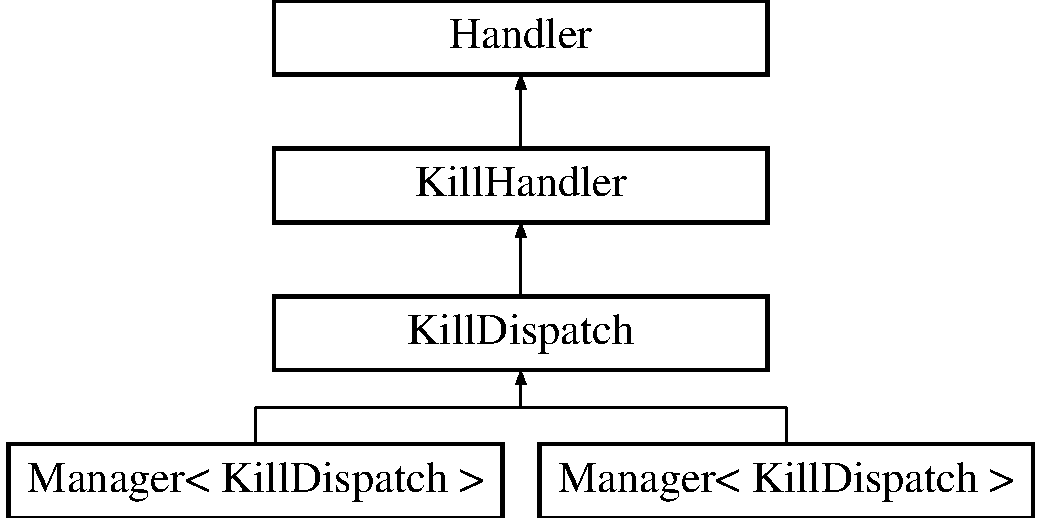
\includegraphics[height=4.000000cm]{class_kill_handler}
\end{center}
\end{figure}
\subsection*{Public Member Functions}
\begin{DoxyCompactItemize}
\item 
void \hyperlink{class_kill_handler_ad5b9007b910c238f62930dc7ba3cf8fc}{on\-Kill} (\hyperlink{class_player}{Player} $\ast$p)
\item 
void \hyperlink{class_kill_handler_a6fa4f74ade6390de9539116dae4359c4}{on\-Kill} (\hyperlink{class_alive}{Alive} $\ast$a)
\item 
void \hyperlink{class_kill_handler_a0da0e64f9ec3eaedd7b6fe2b421e26c8}{on\-Kill} (\hyperlink{class_entity}{Entity} $\ast$e)
\end{DoxyCompactItemize}
\subsection*{Additional Inherited Members}


\subsection{Member Function Documentation}
\hypertarget{class_kill_handler_ad5b9007b910c238f62930dc7ba3cf8fc}{\index{Kill\-Handler@{Kill\-Handler}!on\-Kill@{on\-Kill}}
\index{on\-Kill@{on\-Kill}!KillHandler@{Kill\-Handler}}
\subsubsection[{on\-Kill}]{\setlength{\rightskip}{0pt plus 5cm}void Kill\-Handler\-::on\-Kill (
\begin{DoxyParamCaption}
\item[{{\bf Player} $\ast$}]{p}
\end{DoxyParamCaption}
)}}\label{class_kill_handler_ad5b9007b910c238f62930dc7ba3cf8fc}
\hypertarget{class_kill_handler_a6fa4f74ade6390de9539116dae4359c4}{\index{Kill\-Handler@{Kill\-Handler}!on\-Kill@{on\-Kill}}
\index{on\-Kill@{on\-Kill}!KillHandler@{Kill\-Handler}}
\subsubsection[{on\-Kill}]{\setlength{\rightskip}{0pt plus 5cm}void Kill\-Handler\-::on\-Kill (
\begin{DoxyParamCaption}
\item[{{\bf Alive} $\ast$}]{a}
\end{DoxyParamCaption}
)}}\label{class_kill_handler_a6fa4f74ade6390de9539116dae4359c4}
\hypertarget{class_kill_handler_a0da0e64f9ec3eaedd7b6fe2b421e26c8}{\index{Kill\-Handler@{Kill\-Handler}!on\-Kill@{on\-Kill}}
\index{on\-Kill@{on\-Kill}!KillHandler@{Kill\-Handler}}
\subsubsection[{on\-Kill}]{\setlength{\rightskip}{0pt plus 5cm}void Kill\-Handler\-::on\-Kill (
\begin{DoxyParamCaption}
\item[{{\bf Entity} $\ast$}]{e}
\end{DoxyParamCaption}
)}}\label{class_kill_handler_a0da0e64f9ec3eaedd7b6fe2b421e26c8}


The documentation for this class was generated from the following files\-:\begin{DoxyCompactItemize}
\item 
events/\hyperlink{killhandler_8h}{killhandler.\-h}\item 
events/\hyperlink{killhandler_8cpp}{killhandler.\-cpp}\end{DoxyCompactItemize}

\hypertarget{class_lethal}{\section{Lethal Class Reference}
\label{class_lethal}\index{Lethal@{Lethal}}
}


{\ttfamily \#include $<$lethal.\-h$>$}

Inheritance diagram for Lethal\-:\begin{figure}[H]
\begin{center}
\leavevmode
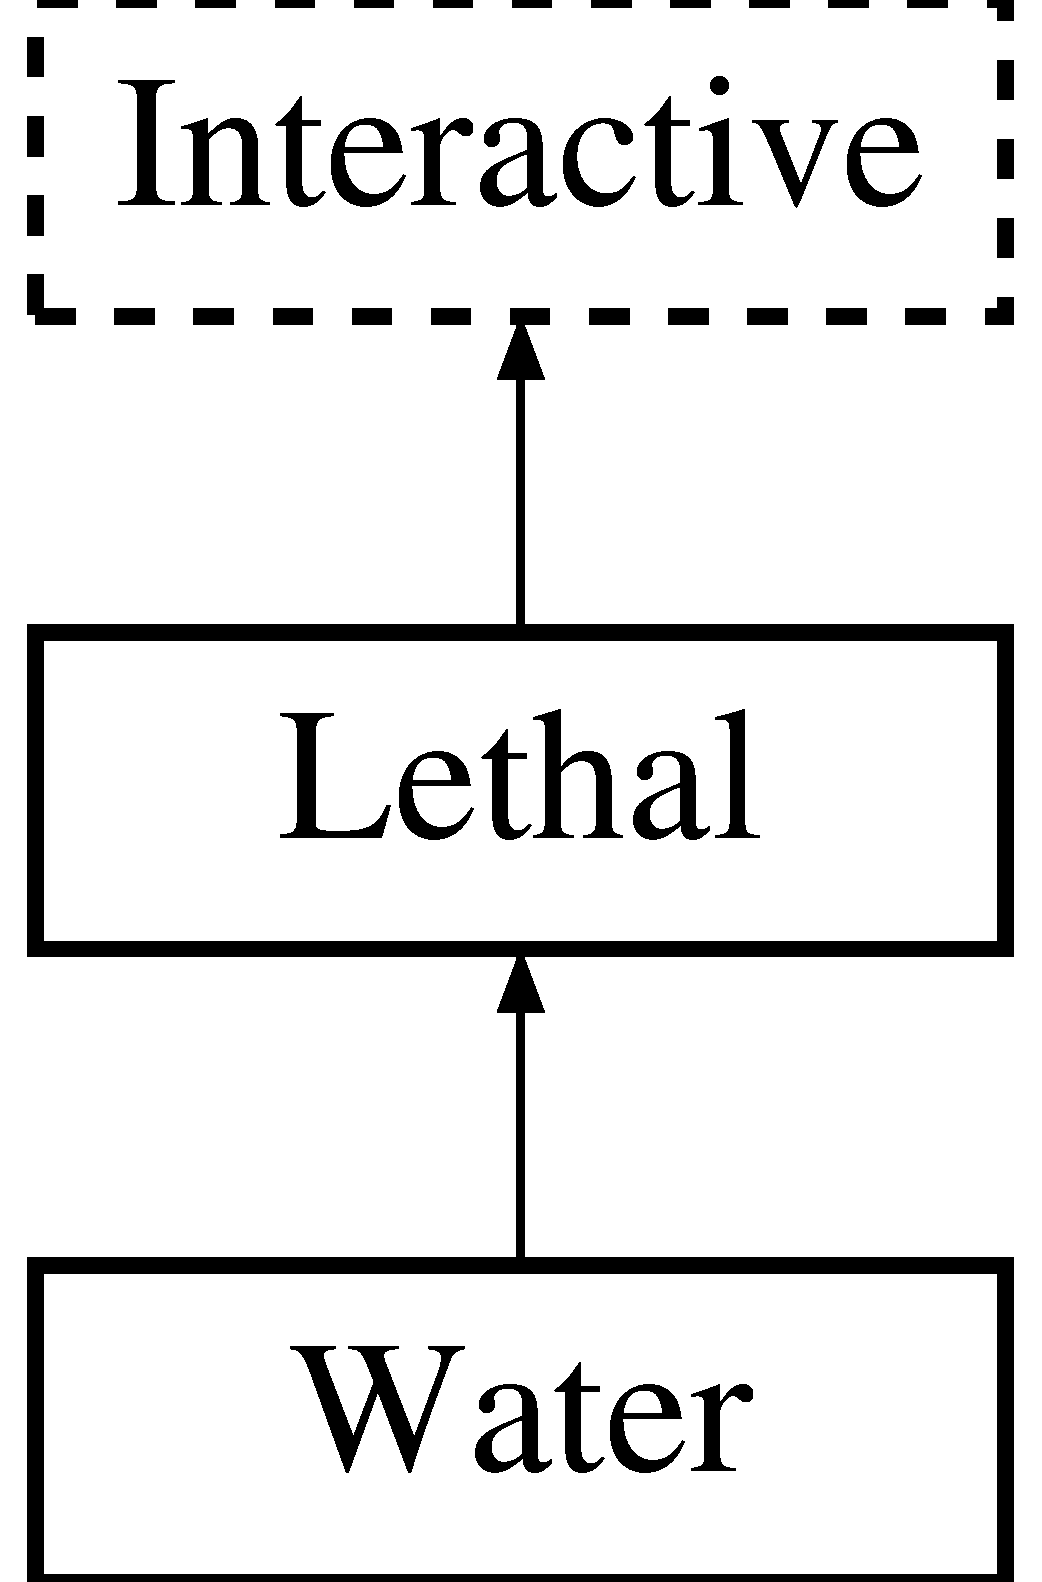
\includegraphics[height=3.000000cm]{class_lethal}
\end{center}
\end{figure}
\subsection*{Additional Inherited Members}


The documentation for this class was generated from the following file\-:\begin{DoxyCompactItemize}
\item 
entities/ia/\hyperlink{lethal_8h}{lethal.\-h}\end{DoxyCompactItemize}

\hypertarget{class_life}{\section{Life Class Reference}
\label{class_life}\index{Life@{Life}}
}


{\ttfamily \#include $<$life.\-h$>$}

Inheritance diagram for Life\-:\begin{figure}[H]
\begin{center}
\leavevmode
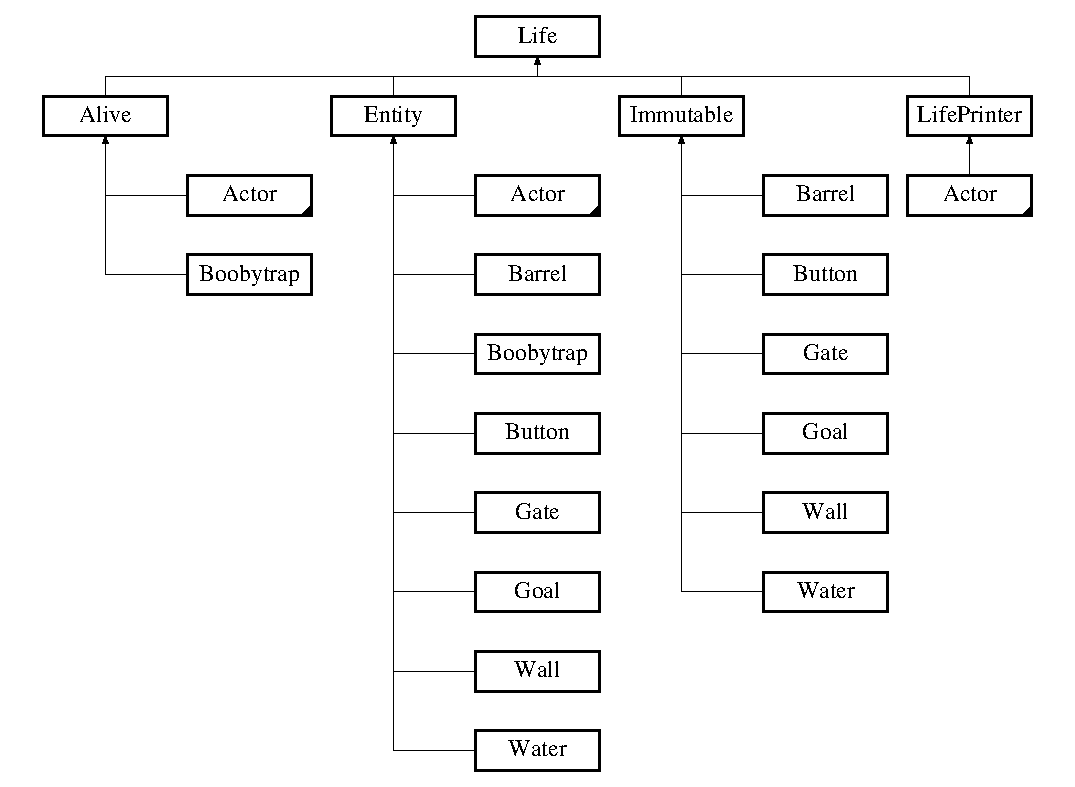
\includegraphics[height=10.000000cm]{class_life}
\end{center}
\end{figure}
\subsection*{Public Member Functions}
\begin{DoxyCompactItemize}
\item 
virtual void \hyperlink{class_life_abe871acf504c14c9c0651e0cad70aaf2}{\-\_\-\-\_\-polymorphic\-\_\-\-\_\-} ()
\item 
virtual bool \hyperlink{class_life_a8f79fb2cb57ef2a76e0c0feba345c68c}{is\-\_\-alive} ()=0
\item 
virtual void \hyperlink{class_life_a40b24b079b08e3a80a582eff6be8faa3}{kill} ()=0
\item 
virtual \hyperlink{class_life_ae236ea616d5a196a1f6b27d789c52fc5}{$\sim$\-Life} ()
\end{DoxyCompactItemize}


\subsection{Constructor \& Destructor Documentation}
\hypertarget{class_life_ae236ea616d5a196a1f6b27d789c52fc5}{\index{Life@{Life}!$\sim$\-Life@{$\sim$\-Life}}
\index{$\sim$\-Life@{$\sim$\-Life}!Life@{Life}}
\subsubsection[{$\sim$\-Life}]{\setlength{\rightskip}{0pt plus 5cm}virtual Life\-::$\sim$\-Life (
\begin{DoxyParamCaption}
{}
\end{DoxyParamCaption}
)\hspace{0.3cm}{\ttfamily [inline]}, {\ttfamily [virtual]}}}\label{class_life_ae236ea616d5a196a1f6b27d789c52fc5}


\subsection{Member Function Documentation}
\hypertarget{class_life_abe871acf504c14c9c0651e0cad70aaf2}{\index{Life@{Life}!\-\_\-\-\_\-polymorphic\-\_\-\-\_\-@{\-\_\-\-\_\-polymorphic\-\_\-\-\_\-}}
\index{\-\_\-\-\_\-polymorphic\-\_\-\-\_\-@{\-\_\-\-\_\-polymorphic\-\_\-\-\_\-}!Life@{Life}}
\subsubsection[{\-\_\-\-\_\-polymorphic\-\_\-\-\_\-}]{\setlength{\rightskip}{0pt plus 5cm}virtual void Life\-::\-\_\-\-\_\-polymorphic\-\_\-\-\_\- (
\begin{DoxyParamCaption}
{}
\end{DoxyParamCaption}
)\hspace{0.3cm}{\ttfamily [inline]}, {\ttfamily [virtual]}}}\label{class_life_abe871acf504c14c9c0651e0cad70aaf2}


Reimplemented in \hyperlink{class_entity_a11d5655c6e057fb86551402380009c01}{Entity}.

\hypertarget{class_life_a8f79fb2cb57ef2a76e0c0feba345c68c}{\index{Life@{Life}!is\-\_\-alive@{is\-\_\-alive}}
\index{is\-\_\-alive@{is\-\_\-alive}!Life@{Life}}
\subsubsection[{is\-\_\-alive}]{\setlength{\rightskip}{0pt plus 5cm}virtual bool Life\-::is\-\_\-alive (
\begin{DoxyParamCaption}
{}
\end{DoxyParamCaption}
)\hspace{0.3cm}{\ttfamily [pure virtual]}}}\label{class_life_a8f79fb2cb57ef2a76e0c0feba345c68c}


Implemented in \hyperlink{class_alive_a35db3016aaa9bbea5e9bcaa4965581b6}{Alive}, and \hyperlink{class_immutable_a0460b0dffb45031b03bb1835a86c3185}{Immutable}.

\hypertarget{class_life_a40b24b079b08e3a80a582eff6be8faa3}{\index{Life@{Life}!kill@{kill}}
\index{kill@{kill}!Life@{Life}}
\subsubsection[{kill}]{\setlength{\rightskip}{0pt plus 5cm}virtual void Life\-::kill (
\begin{DoxyParamCaption}
{}
\end{DoxyParamCaption}
)\hspace{0.3cm}{\ttfamily [pure virtual]}}}\label{class_life_a40b24b079b08e3a80a582eff6be8faa3}


Implemented in \hyperlink{class_alive_aa10e42533e1f6277ce7da1ca9a2d0b71}{Alive}, and \hyperlink{class_immutable_ad74ffebf832d588e19e3746c09c90d1a}{Immutable}.



The documentation for this class was generated from the following file\-:\begin{DoxyCompactItemize}
\item 
entities/life/\hyperlink{life_8h}{life.\-h}\end{DoxyCompactItemize}

\hypertarget{class_life_printer}{\section{Life\-Printer Class Reference}
\label{class_life_printer}\index{Life\-Printer@{Life\-Printer}}
}


{\ttfamily \#include $<$lifeprinter.\-h$>$}

Inheritance diagram for Life\-Printer\-:\begin{figure}[H]
\begin{center}
\leavevmode
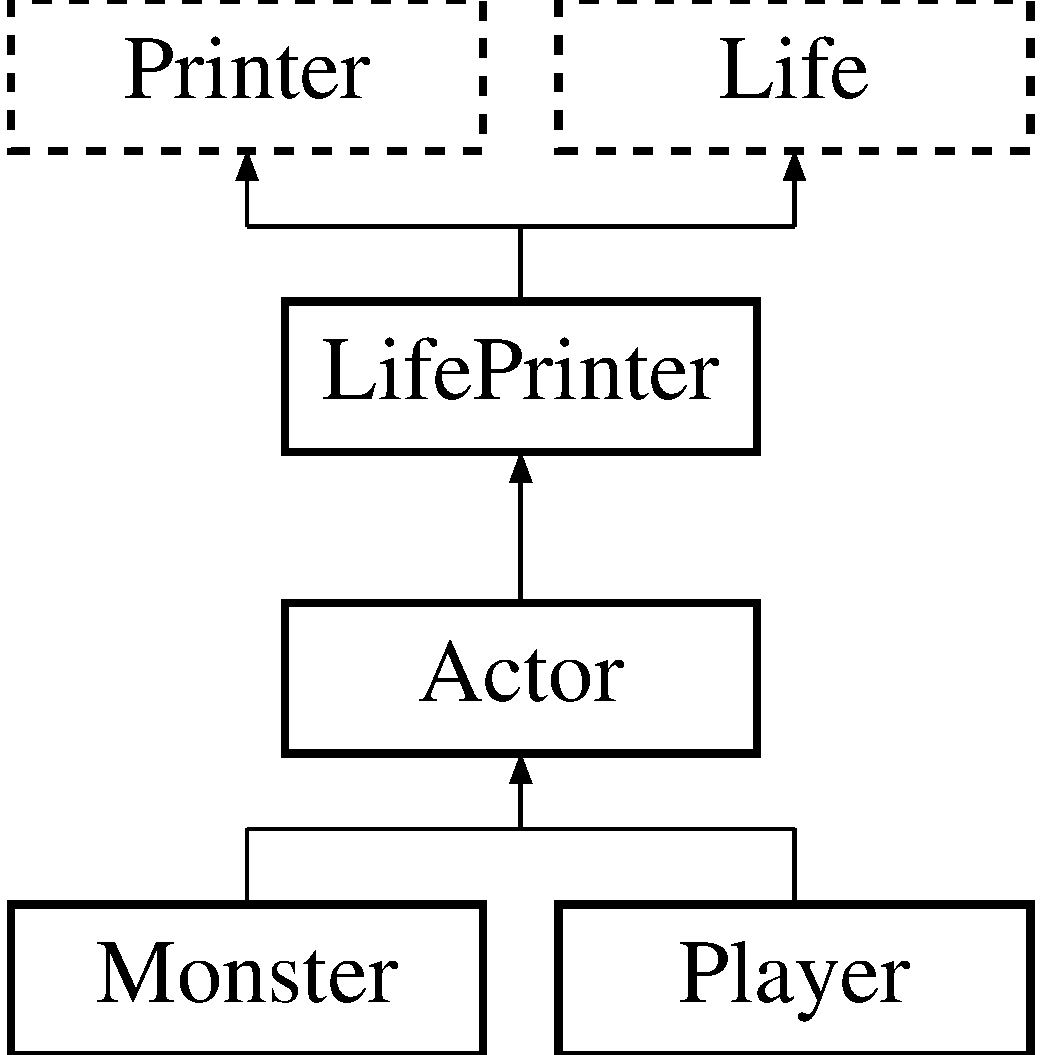
\includegraphics[height=4.000000cm]{class_life_printer}
\end{center}
\end{figure}
\subsection*{Public Member Functions}
\begin{DoxyCompactItemize}
\item 
\hyperlink{class_life_printer_a6693ebbe13889415345d4e9ad0618f75}{Life\-Printer} (char \-\_\-alive, char \-\_\-dead)
\item 
char \hyperlink{class_life_printer_ab62c96990f0f0f605255e3394d64246b}{to\-\_\-char} ()
\end{DoxyCompactItemize}


\subsection{Constructor \& Destructor Documentation}
\hypertarget{class_life_printer_a6693ebbe13889415345d4e9ad0618f75}{\index{Life\-Printer@{Life\-Printer}!Life\-Printer@{Life\-Printer}}
\index{Life\-Printer@{Life\-Printer}!LifePrinter@{Life\-Printer}}
\subsubsection[{Life\-Printer}]{\setlength{\rightskip}{0pt plus 5cm}Life\-Printer\-::\-Life\-Printer (
\begin{DoxyParamCaption}
\item[{char}]{\-\_\-alive, }
\item[{char}]{\-\_\-dead}
\end{DoxyParamCaption}
)}}\label{class_life_printer_a6693ebbe13889415345d4e9ad0618f75}


\subsection{Member Function Documentation}
\hypertarget{class_life_printer_ab62c96990f0f0f605255e3394d64246b}{\index{Life\-Printer@{Life\-Printer}!to\-\_\-char@{to\-\_\-char}}
\index{to\-\_\-char@{to\-\_\-char}!LifePrinter@{Life\-Printer}}
\subsubsection[{to\-\_\-char}]{\setlength{\rightskip}{0pt plus 5cm}char Life\-Printer\-::to\-\_\-char (
\begin{DoxyParamCaption}
{}
\end{DoxyParamCaption}
)\hspace{0.3cm}{\ttfamily [virtual]}}}\label{class_life_printer_ab62c96990f0f0f605255e3394d64246b}


Implements \hyperlink{class_printer_a66ecfd99bb8bc0a88ed0fc1276c70e23}{Printer}.



The documentation for this class was generated from the following files\-:\begin{DoxyCompactItemize}
\item 
entities/printer/\hyperlink{lifeprinter_8h}{lifeprinter.\-h}\item 
entities/printer/\hyperlink{lifeprinter_8cpp}{lifeprinter.\-cpp}\end{DoxyCompactItemize}

\hypertarget{class_manager}{\section{Manager$<$ Dispatcher\-T $>$ Class Template Reference}
\label{class_manager}\index{Manager$<$ Dispatcher\-T $>$@{Manager$<$ Dispatcher\-T $>$}}
}


{\ttfamily \#include $<$collisionmanager.\-h$>$}

Inheritance diagram for Manager$<$ Dispatcher\-T $>$\-:\begin{figure}[H]
\begin{center}
\leavevmode
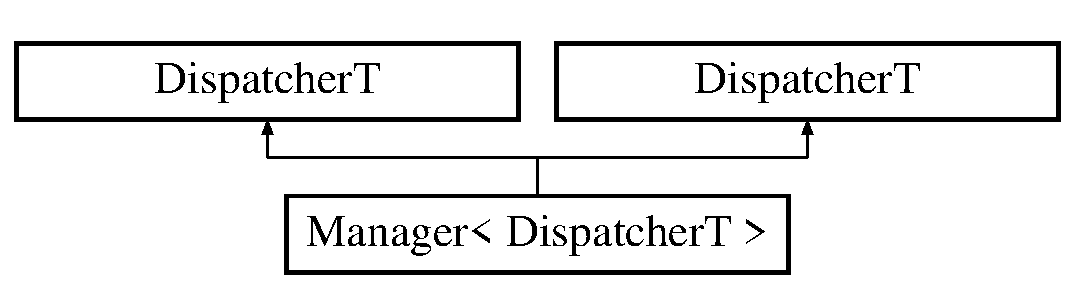
\includegraphics[height=2.000000cm]{class_manager}
\end{center}
\end{figure}
\subsection*{Public Member Functions}
\begin{DoxyCompactItemize}
\item 
\hyperlink{class_manager_acf4518aae98aa841e94511ad59d105a4}{Manager} (\hyperlink{class_game}{Game} $\ast$\-\_\-g)
\item 
\hyperlink{class_manager_acf4518aae98aa841e94511ad59d105a4}{Manager} (\hyperlink{class_game}{Game} $\ast$\-\_\-g)
\end{DoxyCompactItemize}


\subsection{Constructor \& Destructor Documentation}
\hypertarget{class_manager_acf4518aae98aa841e94511ad59d105a4}{\index{Manager@{Manager}!Manager@{Manager}}
\index{Manager@{Manager}!Manager@{Manager}}
\subsubsection[{Manager}]{\setlength{\rightskip}{0pt plus 5cm}template$<$typename Dispatcher\-T$>$ {\bf Manager}$<$ Dispatcher\-T $>$\-::{\bf Manager} (
\begin{DoxyParamCaption}
\item[{{\bf Game} $\ast$}]{\-\_\-g}
\end{DoxyParamCaption}
)\hspace{0.3cm}{\ttfamily [inline]}}}\label{class_manager_acf4518aae98aa841e94511ad59d105a4}
\hypertarget{class_manager_acf4518aae98aa841e94511ad59d105a4}{\index{Manager@{Manager}!Manager@{Manager}}
\index{Manager@{Manager}!Manager@{Manager}}
\subsubsection[{Manager}]{\setlength{\rightskip}{0pt plus 5cm}template$<$typename Dispatcher\-T$>$ {\bf Manager}$<$ Dispatcher\-T $>$\-::{\bf Manager} (
\begin{DoxyParamCaption}
\item[{{\bf Game} $\ast$}]{\-\_\-g}
\end{DoxyParamCaption}
)\hspace{0.3cm}{\ttfamily [inline]}}}\label{class_manager_acf4518aae98aa841e94511ad59d105a4}


The documentation for this class was generated from the following files\-:\begin{DoxyCompactItemize}
\item 
events/\hyperlink{collisionmanager_8h}{collisionmanager.\-h}\item 
events/\hyperlink{managers_8h}{managers.\-h}\end{DoxyCompactItemize}

\hypertarget{class_monster}{\section{Monster Class Reference}
\label{class_monster}\index{Monster@{Monster}}
}


{\ttfamily \#include $<$monster.\-h$>$}

Inheritance diagram for Monster\-:\begin{figure}[H]
\begin{center}
\leavevmode
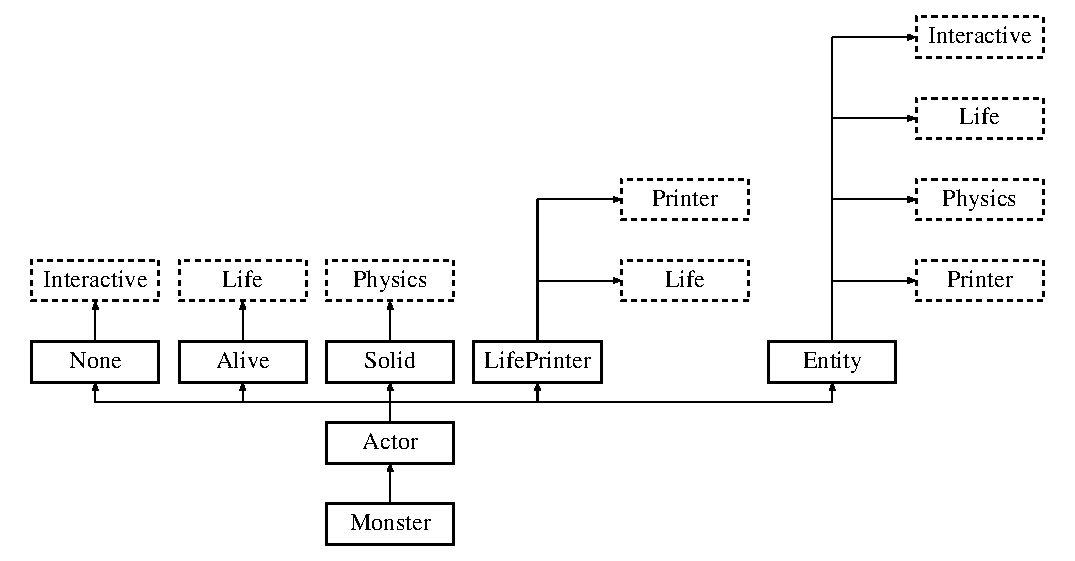
\includegraphics[height=7.000000cm]{class_monster}
\end{center}
\end{figure}
\subsection*{Public Member Functions}
\begin{DoxyCompactItemize}
\item 
\hyperlink{class_monster_ad8caa528485f4c09b84ae04fca59d786}{Monster} (unsigned int \hyperlink{class_entity_afa8f48eccdb09a290e2c1ded3f135363}{x}, unsigned \hyperlink{class_entity_a9d39843430829a89bb8233dbaadae4f1}{y}, std\-::string \-\_\-name)
\item 
void \hyperlink{class_monster_aba6f66599146c238ff906e0bffb06b71}{info} (std\-::ostream \&out)
\end{DoxyCompactItemize}
\subsection*{Additional Inherited Members}


\subsection{Constructor \& Destructor Documentation}
\hypertarget{class_monster_ad8caa528485f4c09b84ae04fca59d786}{\index{Monster@{Monster}!Monster@{Monster}}
\index{Monster@{Monster}!Monster@{Monster}}
\subsubsection[{Monster}]{\setlength{\rightskip}{0pt plus 5cm}Monster\-::\-Monster (
\begin{DoxyParamCaption}
\item[{unsigned int}]{x, }
\item[{unsigned}]{y, }
\item[{std\-::string}]{\-\_\-name}
\end{DoxyParamCaption}
)}}\label{class_monster_ad8caa528485f4c09b84ae04fca59d786}
E\-N\-S\-U\-R\-E(\hyperlink{class_entity_af7f20142aa7883ca29a91c43e3511e48}{properly\-Initialized()}, \char`\"{}\-Constructor must end...\char`\"{}) 

\subsection{Member Function Documentation}
\hypertarget{class_monster_aba6f66599146c238ff906e0bffb06b71}{\index{Monster@{Monster}!info@{info}}
\index{info@{info}!Monster@{Monster}}
\subsubsection[{info}]{\setlength{\rightskip}{0pt plus 5cm}void Monster\-::info (
\begin{DoxyParamCaption}
\item[{std\-::ostream \&}]{out}
\end{DoxyParamCaption}
)\hspace{0.3cm}{\ttfamily [virtual]}}}\label{class_monster_aba6f66599146c238ff906e0bffb06b71}
R\-E\-Q\-U\-I\-R\-E(\hyperlink{class_entity_af7f20142aa7883ca29a91c43e3511e48}{properly\-Initialized()}, \char`\"{}\-Monster wasn't initialized when calling info\char`\"{}) 

Implements \hyperlink{class_entity_aa694874d1f59971187de675d1e0c1fdf}{Entity}.



The documentation for this class was generated from the following files\-:\begin{DoxyCompactItemize}
\item 
entities/\hyperlink{monster_8h}{monster.\-h}\item 
entities/\hyperlink{monster_8cpp}{monster.\-cpp}\end{DoxyCompactItemize}

\hypertarget{class_move}{\section{Move Class Reference}
\label{class_move}\index{Move@{Move}}
}


{\ttfamily \#include $<$move.\-h$>$}

Inheritance diagram for Move\-:\begin{figure}[H]
\begin{center}
\leavevmode
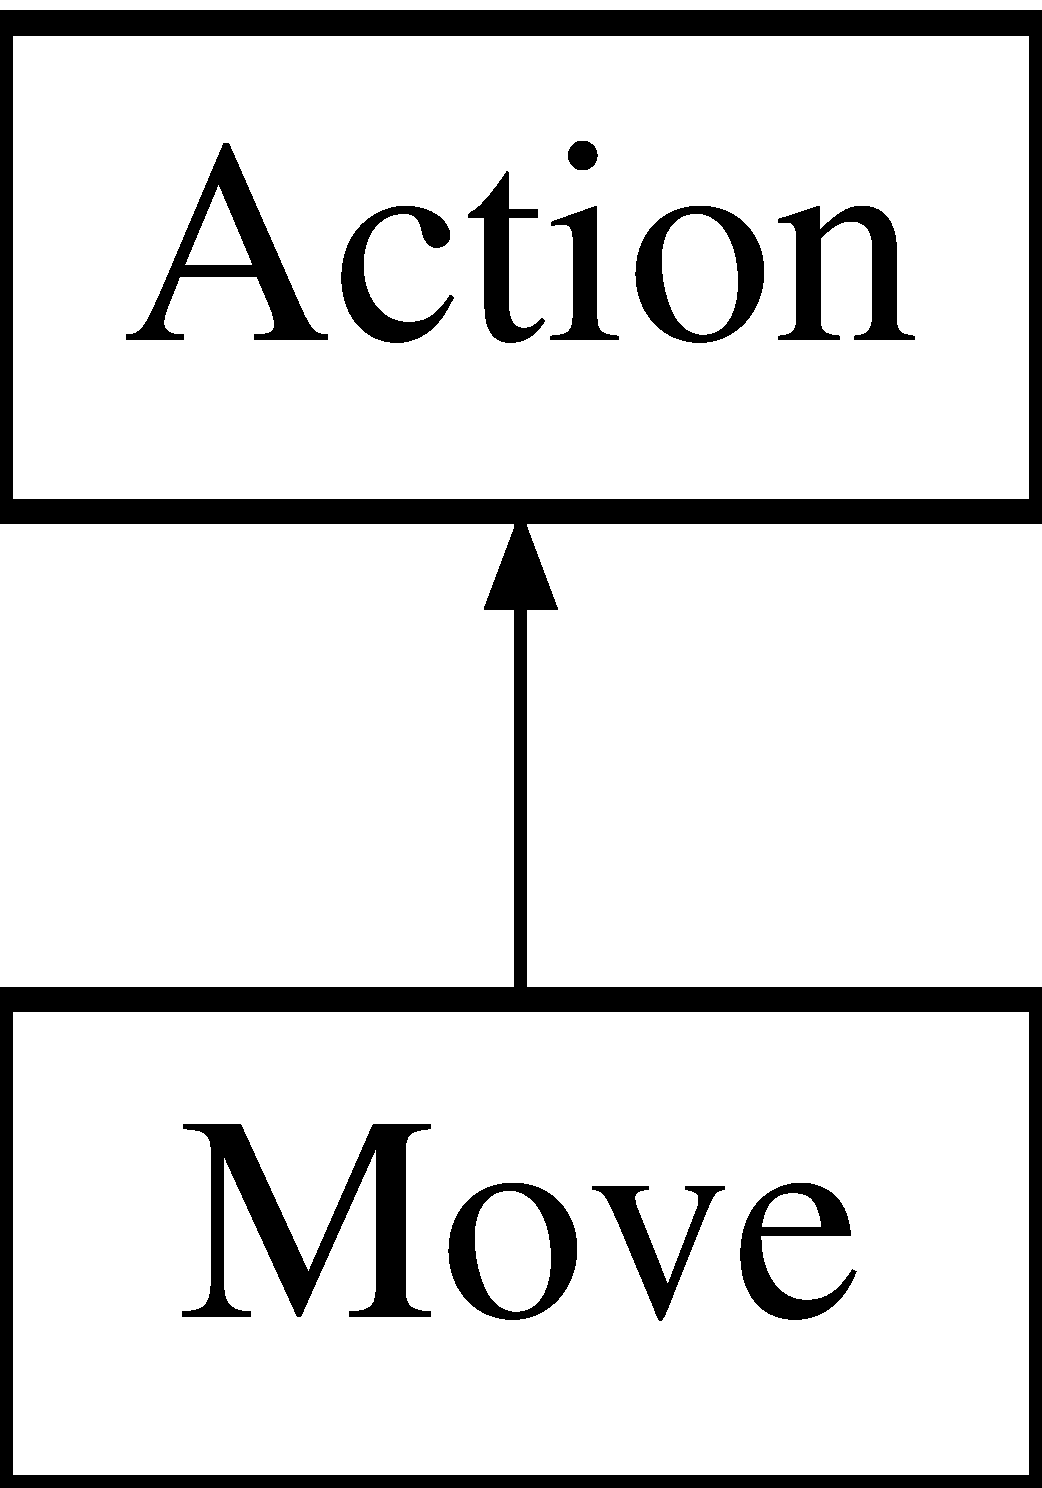
\includegraphics[height=2.000000cm]{class_move}
\end{center}
\end{figure}
\subsection*{Public Member Functions}
\begin{DoxyCompactItemize}
\item 
\hyperlink{class_move_a4713df2a93055e6aa8c6b4d84ab17e0b}{Move} (\hyperlink{class_actor}{Actor} $\ast$\-\_\-actor, std\-::string \&dirname)
\item 
bool \hyperlink{class_move_a3fbaa547d4a9f9311a326d584c6c0de5}{execute} (\hyperlink{class_game}{Game} $\ast$g)
\end{DoxyCompactItemize}
\subsection*{Additional Inherited Members}


\subsection{Constructor \& Destructor Documentation}
\hypertarget{class_move_a4713df2a93055e6aa8c6b4d84ab17e0b}{\index{Move@{Move}!Move@{Move}}
\index{Move@{Move}!Move@{Move}}
\subsubsection[{Move}]{\setlength{\rightskip}{0pt plus 5cm}Move\-::\-Move (
\begin{DoxyParamCaption}
\item[{{\bf Actor} $\ast$}]{\-\_\-actor, }
\item[{std\-::string \&}]{dirname}
\end{DoxyParamCaption}
)}}\label{class_move_a4713df2a93055e6aa8c6b4d84ab17e0b}


\subsection{Member Function Documentation}
\hypertarget{class_move_a3fbaa547d4a9f9311a326d584c6c0de5}{\index{Move@{Move}!execute@{execute}}
\index{execute@{execute}!Move@{Move}}
\subsubsection[{execute}]{\setlength{\rightskip}{0pt plus 5cm}bool Move\-::execute (
\begin{DoxyParamCaption}
\item[{{\bf Game} $\ast$}]{g}
\end{DoxyParamCaption}
)\hspace{0.3cm}{\ttfamily [virtual]}}}\label{class_move_a3fbaa547d4a9f9311a326d584c6c0de5}


Implements \hyperlink{class_action_a18a2520db7750f26d7a571c990b82daf}{Action}.



The documentation for this class was generated from the following files\-:\begin{DoxyCompactItemize}
\item 
actions/\hyperlink{move_8h}{move.\-h}\item 
actions/\hyperlink{move_8cpp}{move.\-cpp}\end{DoxyCompactItemize}

\hypertarget{class_none}{\section{None Class Reference}
\label{class_none}\index{None@{None}}
}


{\ttfamily \#include $<$none.\-h$>$}

Inheritance diagram for None\-:\begin{figure}[H]
\begin{center}
\leavevmode
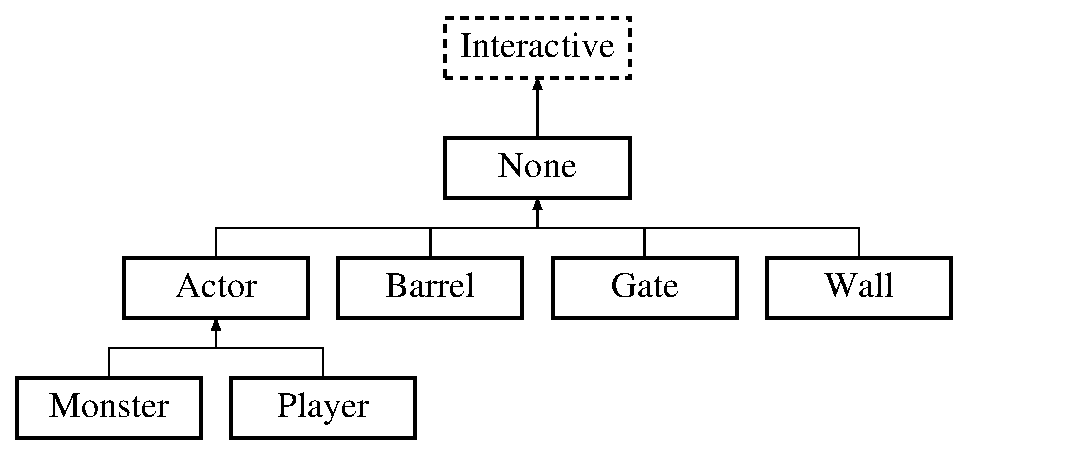
\includegraphics[height=4.000000cm]{class_none}
\end{center}
\end{figure}
\subsection*{Additional Inherited Members}


The documentation for this class was generated from the following file\-:\begin{DoxyCompactItemize}
\item 
entities/ia/\hyperlink{none_8h}{none.\-h}\end{DoxyCompactItemize}

\hypertarget{class_parse_error}{\section{Parse\-Error Class Reference}
\label{class_parse_error}\index{Parse\-Error@{Parse\-Error}}
}


{\ttfamily \#include $<$parser.\-h$>$}

Inheritance diagram for Parse\-Error\-:\begin{figure}[H]
\begin{center}
\leavevmode
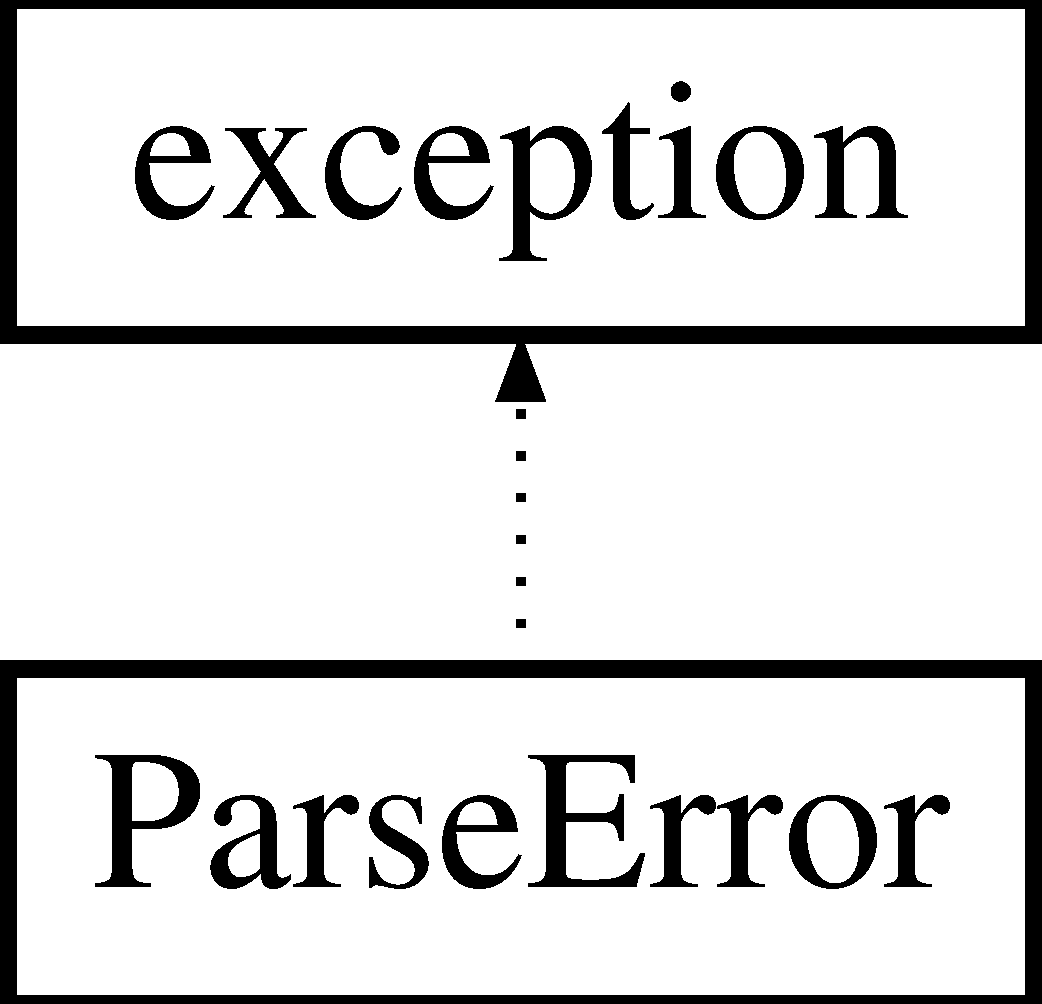
\includegraphics[height=2.000000cm]{class_parse_error}
\end{center}
\end{figure}
\subsection*{Public Member Functions}
\begin{DoxyCompactItemize}
\item 
\hyperlink{class_parse_error_a1db9c9dad671ad0a22cb04afa5df6be2}{Parse\-Error} (std\-::string info, std\-::string filename)
\item 
const char $\ast$ \hyperlink{class_parse_error_aeaca4de4aa07b84893eecbb19b540a3c}{what} ()  throw ()
\end{DoxyCompactItemize}


\subsection{Constructor \& Destructor Documentation}
\hypertarget{class_parse_error_a1db9c9dad671ad0a22cb04afa5df6be2}{\index{Parse\-Error@{Parse\-Error}!Parse\-Error@{Parse\-Error}}
\index{Parse\-Error@{Parse\-Error}!ParseError@{Parse\-Error}}
\subsubsection[{Parse\-Error}]{\setlength{\rightskip}{0pt plus 5cm}Parse\-Error\-::\-Parse\-Error (
\begin{DoxyParamCaption}
\item[{std\-::string}]{info, }
\item[{std\-::string}]{filename}
\end{DoxyParamCaption}
)\hspace{0.3cm}{\ttfamily [inline]}}}\label{class_parse_error_a1db9c9dad671ad0a22cb04afa5df6be2}


\subsection{Member Function Documentation}
\hypertarget{class_parse_error_aeaca4de4aa07b84893eecbb19b540a3c}{\index{Parse\-Error@{Parse\-Error}!what@{what}}
\index{what@{what}!ParseError@{Parse\-Error}}
\subsubsection[{what}]{\setlength{\rightskip}{0pt plus 5cm}const char$\ast$ Parse\-Error\-::what (
\begin{DoxyParamCaption}
{}
\end{DoxyParamCaption}
) throw  ) \hspace{0.3cm}{\ttfamily [inline]}}}\label{class_parse_error_aeaca4de4aa07b84893eecbb19b540a3c}


The documentation for this class was generated from the following file\-:\begin{DoxyCompactItemize}
\item 
parsers/\hyperlink{parser_8h}{parser.\-h}\end{DoxyCompactItemize}

\hypertarget{class_parser}{\section{Parser Class Reference}
\label{class_parser}\index{Parser@{Parser}}
}


{\ttfamily \#include $<$parser.\-h$>$}

Inheritance diagram for Parser\-:\begin{figure}[H]
\begin{center}
\leavevmode
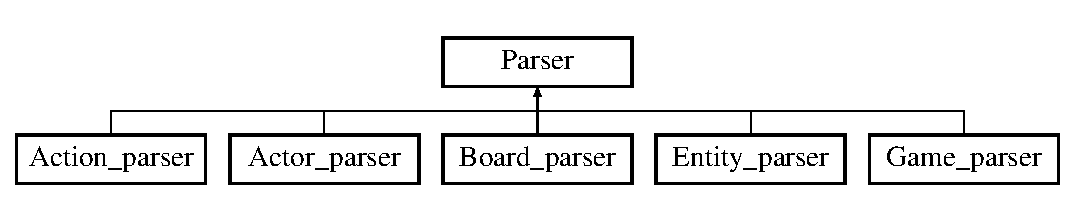
\includegraphics[height=2.000000cm]{class_parser}
\end{center}
\end{figure}
\subsection*{Public Member Functions}
\begin{DoxyCompactItemize}
\item 
\hyperlink{class_parser_a12234f6cd36b61af4b50c94a179422c1}{Parser} ()
\item 
\hyperlink{class_parser_a89acc6fb3df6ab8e057f43d065c1ff50}{Parser} (std\-::ostream $\ast$stream, std\-::string filename=\char`\"{}U\-N\-K\-N\-O\-W\-N\char`\"{})
\item 
void \hyperlink{class_parser_a5bd88cd16274ffe89c0a5ec0678525da}{set\-\_\-out} (std\-::ostream $\ast$stream)
\end{DoxyCompactItemize}
\subsection*{Protected Member Functions}
\begin{DoxyCompactItemize}
\item 
void \hyperlink{class_parser_ae8eeb9f3116dce90f8fd5ab267c5773f}{format\-\_\-message} (std\-::string \&msg, Ti\-Xml\-Base $\ast$el)
\item 
void \hyperlink{class_parser_ae4c1362cb6fe05ba3eb3f1e662654a7c}{log} (std\-::string msg, Ti\-Xml\-Base $\ast$el=nullptr)
\item 
void \hyperlink{class_parser_abc90ea43684459b62e7c6e427a837840}{fatal} (std\-::string msg, Ti\-Xml\-Base $\ast$el=nullptr)
\item 
std\-::string \hyperlink{class_parser_a977153b2f9ff5be8cf436696b18e4c6c}{read\-Element} (Ti\-Xml\-Element $\ast$elem, const char $\ast$tag)
\item 
std\-::string \hyperlink{class_parser_ad6ad607bb6ca701cdaba3dbea8d26ca6}{read\-Element} (Ti\-Xml\-Element $\ast$elem)
\item 
std\-::string \hyperlink{class_parser_ab9e0267aecaf7861b8a239fb72da949b}{read\-Attribute} (Ti\-Xml\-Element $\ast$elem, const char $\ast$tag)
\item 
bool \hyperlink{class_parser_a44cf607802b6863b512ccdbe6c34c9ad}{req\-Element} (Ti\-Xml\-Element $\ast$elem, const char $\ast$tag)
\end{DoxyCompactItemize}
\subsection*{Protected Attributes}
\begin{DoxyCompactItemize}
\item 
std\-::ostream $\ast$ \hyperlink{class_parser_a9d7a3f96e466a7a28a5402283b842341}{\-\_\-out}
\item 
std\-::string \hyperlink{class_parser_a41c96386f1b315f661dbaeca8b230090}{\-\_\-filename}
\end{DoxyCompactItemize}


\subsection{Constructor \& Destructor Documentation}
\hypertarget{class_parser_a12234f6cd36b61af4b50c94a179422c1}{\index{Parser@{Parser}!Parser@{Parser}}
\index{Parser@{Parser}!Parser@{Parser}}
\subsubsection[{Parser}]{\setlength{\rightskip}{0pt plus 5cm}Parser\-::\-Parser (
\begin{DoxyParamCaption}
{}
\end{DoxyParamCaption}
)}}\label{class_parser_a12234f6cd36b61af4b50c94a179422c1}
\hypertarget{class_parser_a89acc6fb3df6ab8e057f43d065c1ff50}{\index{Parser@{Parser}!Parser@{Parser}}
\index{Parser@{Parser}!Parser@{Parser}}
\subsubsection[{Parser}]{\setlength{\rightskip}{0pt plus 5cm}Parser\-::\-Parser (
\begin{DoxyParamCaption}
\item[{std\-::ostream $\ast$}]{stream, }
\item[{std\-::string}]{filename = {\ttfamily \char`\"{}UNKNOWN\char`\"{}}}
\end{DoxyParamCaption}
)}}\label{class_parser_a89acc6fb3df6ab8e057f43d065c1ff50}


\subsection{Member Function Documentation}
\hypertarget{class_parser_abc90ea43684459b62e7c6e427a837840}{\index{Parser@{Parser}!fatal@{fatal}}
\index{fatal@{fatal}!Parser@{Parser}}
\subsubsection[{fatal}]{\setlength{\rightskip}{0pt plus 5cm}void Parser\-::fatal (
\begin{DoxyParamCaption}
\item[{std\-::string}]{msg, }
\item[{Ti\-Xml\-Base $\ast$}]{el = {\ttfamily nullptr}}
\end{DoxyParamCaption}
)\hspace{0.3cm}{\ttfamily [protected]}}}\label{class_parser_abc90ea43684459b62e7c6e427a837840}
\hypertarget{class_parser_ae8eeb9f3116dce90f8fd5ab267c5773f}{\index{Parser@{Parser}!format\-\_\-message@{format\-\_\-message}}
\index{format\-\_\-message@{format\-\_\-message}!Parser@{Parser}}
\subsubsection[{format\-\_\-message}]{\setlength{\rightskip}{0pt plus 5cm}void Parser\-::format\-\_\-message (
\begin{DoxyParamCaption}
\item[{std\-::string \&}]{msg, }
\item[{Ti\-Xml\-Base $\ast$}]{el}
\end{DoxyParamCaption}
)\hspace{0.3cm}{\ttfamily [protected]}}}\label{class_parser_ae8eeb9f3116dce90f8fd5ab267c5773f}
\hypertarget{class_parser_ae4c1362cb6fe05ba3eb3f1e662654a7c}{\index{Parser@{Parser}!log@{log}}
\index{log@{log}!Parser@{Parser}}
\subsubsection[{log}]{\setlength{\rightskip}{0pt plus 5cm}void Parser\-::log (
\begin{DoxyParamCaption}
\item[{std\-::string}]{msg, }
\item[{Ti\-Xml\-Base $\ast$}]{el = {\ttfamily nullptr}}
\end{DoxyParamCaption}
)\hspace{0.3cm}{\ttfamily [protected]}}}\label{class_parser_ae4c1362cb6fe05ba3eb3f1e662654a7c}
\hypertarget{class_parser_ab9e0267aecaf7861b8a239fb72da949b}{\index{Parser@{Parser}!read\-Attribute@{read\-Attribute}}
\index{read\-Attribute@{read\-Attribute}!Parser@{Parser}}
\subsubsection[{read\-Attribute}]{\setlength{\rightskip}{0pt plus 5cm}std\-::string Parser\-::read\-Attribute (
\begin{DoxyParamCaption}
\item[{Ti\-Xml\-Element $\ast$}]{elem, }
\item[{const char $\ast$}]{tag}
\end{DoxyParamCaption}
)\hspace{0.3cm}{\ttfamily [protected]}}}\label{class_parser_ab9e0267aecaf7861b8a239fb72da949b}
\hypertarget{class_parser_a977153b2f9ff5be8cf436696b18e4c6c}{\index{Parser@{Parser}!read\-Element@{read\-Element}}
\index{read\-Element@{read\-Element}!Parser@{Parser}}
\subsubsection[{read\-Element}]{\setlength{\rightskip}{0pt plus 5cm}std\-::string Parser\-::read\-Element (
\begin{DoxyParamCaption}
\item[{Ti\-Xml\-Element $\ast$}]{elem, }
\item[{const char $\ast$}]{tag}
\end{DoxyParamCaption}
)\hspace{0.3cm}{\ttfamily [protected]}}}\label{class_parser_a977153b2f9ff5be8cf436696b18e4c6c}
\hypertarget{class_parser_ad6ad607bb6ca701cdaba3dbea8d26ca6}{\index{Parser@{Parser}!read\-Element@{read\-Element}}
\index{read\-Element@{read\-Element}!Parser@{Parser}}
\subsubsection[{read\-Element}]{\setlength{\rightskip}{0pt plus 5cm}std\-::string Parser\-::read\-Element (
\begin{DoxyParamCaption}
\item[{Ti\-Xml\-Element $\ast$}]{elem}
\end{DoxyParamCaption}
)\hspace{0.3cm}{\ttfamily [protected]}}}\label{class_parser_ad6ad607bb6ca701cdaba3dbea8d26ca6}
\hypertarget{class_parser_a44cf607802b6863b512ccdbe6c34c9ad}{\index{Parser@{Parser}!req\-Element@{req\-Element}}
\index{req\-Element@{req\-Element}!Parser@{Parser}}
\subsubsection[{req\-Element}]{\setlength{\rightskip}{0pt plus 5cm}bool Parser\-::req\-Element (
\begin{DoxyParamCaption}
\item[{Ti\-Xml\-Element $\ast$}]{elem, }
\item[{const char $\ast$}]{tag}
\end{DoxyParamCaption}
)\hspace{0.3cm}{\ttfamily [protected]}}}\label{class_parser_a44cf607802b6863b512ccdbe6c34c9ad}
\hypertarget{class_parser_a5bd88cd16274ffe89c0a5ec0678525da}{\index{Parser@{Parser}!set\-\_\-out@{set\-\_\-out}}
\index{set\-\_\-out@{set\-\_\-out}!Parser@{Parser}}
\subsubsection[{set\-\_\-out}]{\setlength{\rightskip}{0pt plus 5cm}void Parser\-::set\-\_\-out (
\begin{DoxyParamCaption}
\item[{std\-::ostream $\ast$}]{stream}
\end{DoxyParamCaption}
)}}\label{class_parser_a5bd88cd16274ffe89c0a5ec0678525da}


\subsection{Member Data Documentation}
\hypertarget{class_parser_a41c96386f1b315f661dbaeca8b230090}{\index{Parser@{Parser}!\-\_\-filename@{\-\_\-filename}}
\index{\-\_\-filename@{\-\_\-filename}!Parser@{Parser}}
\subsubsection[{\-\_\-filename}]{\setlength{\rightskip}{0pt plus 5cm}std\-::string Parser\-::\-\_\-filename\hspace{0.3cm}{\ttfamily [protected]}}}\label{class_parser_a41c96386f1b315f661dbaeca8b230090}
\hypertarget{class_parser_a9d7a3f96e466a7a28a5402283b842341}{\index{Parser@{Parser}!\-\_\-out@{\-\_\-out}}
\index{\-\_\-out@{\-\_\-out}!Parser@{Parser}}
\subsubsection[{\-\_\-out}]{\setlength{\rightskip}{0pt plus 5cm}std\-::ostream$\ast$ Parser\-::\-\_\-out\hspace{0.3cm}{\ttfamily [protected]}}}\label{class_parser_a9d7a3f96e466a7a28a5402283b842341}


The documentation for this class was generated from the following files\-:\begin{DoxyCompactItemize}
\item 
parsers/\hyperlink{parser_8h}{parser.\-h}\item 
parsers/\hyperlink{parser_8cpp}{parser.\-cpp}\end{DoxyCompactItemize}

\hypertarget{class_physics}{\section{Physics Class Reference}
\label{class_physics}\index{Physics@{Physics}}
}


{\ttfamily \#include $<$physics.\-h$>$}

Inheritance diagram for Physics\-:\begin{figure}[H]
\begin{center}
\leavevmode
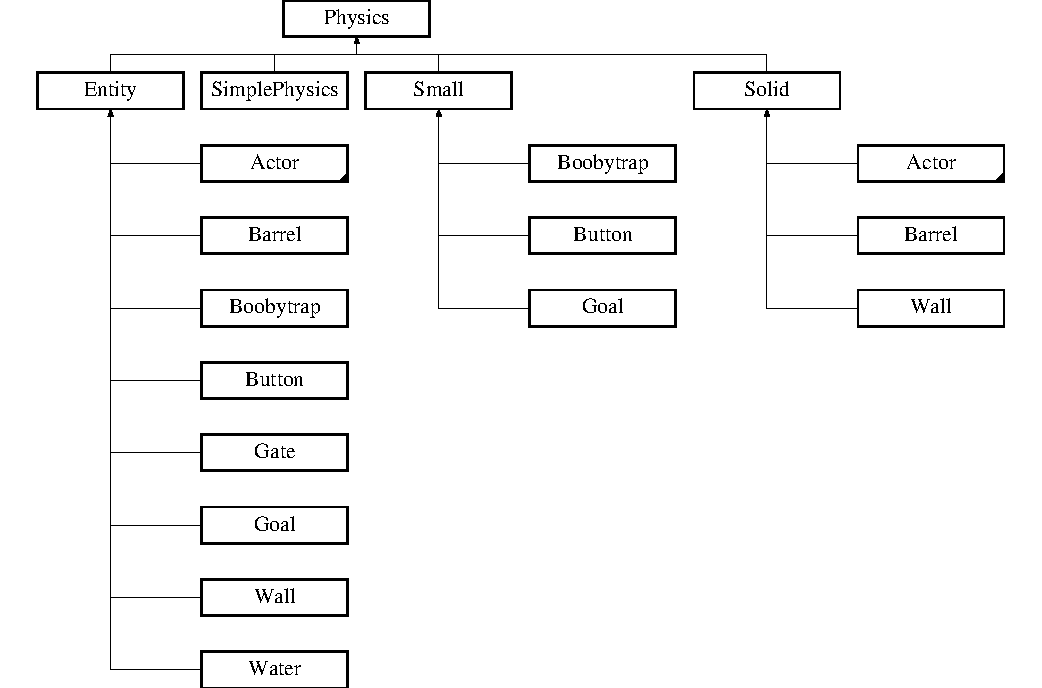
\includegraphics[height=9.240924cm]{class_physics}
\end{center}
\end{figure}
\subsection*{Public Member Functions}
\begin{DoxyCompactItemize}
\item 
virtual void \hyperlink{class_physics_ade73fc725515aeddef262f5b17b1b48c}{\-\_\-\-\_\-polymorphic\-\_\-\-\_\-} ()
\item 
virtual int \hyperlink{class_physics_ae3e59e7723c9f0334b88baf60c01f376}{get\-\_\-height} ()=0
\item 
virtual int \hyperlink{class_physics_a00580cf655d0569cc44f11b630cfcee7}{get\-\_\-weight} ()=0
\item 
virtual \hyperlink{class_physics_afdd87b5bb9fe2e927c37d50fbeb8216b}{$\sim$\-Physics} ()
\end{DoxyCompactItemize}


\subsection{Constructor \& Destructor Documentation}
\hypertarget{class_physics_afdd87b5bb9fe2e927c37d50fbeb8216b}{\index{Physics@{Physics}!$\sim$\-Physics@{$\sim$\-Physics}}
\index{$\sim$\-Physics@{$\sim$\-Physics}!Physics@{Physics}}
\subsubsection[{$\sim$\-Physics}]{\setlength{\rightskip}{0pt plus 5cm}virtual Physics\-::$\sim$\-Physics (
\begin{DoxyParamCaption}
{}
\end{DoxyParamCaption}
)\hspace{0.3cm}{\ttfamily [inline]}, {\ttfamily [virtual]}}}\label{class_physics_afdd87b5bb9fe2e927c37d50fbeb8216b}


\subsection{Member Function Documentation}
\hypertarget{class_physics_ade73fc725515aeddef262f5b17b1b48c}{\index{Physics@{Physics}!\-\_\-\-\_\-polymorphic\-\_\-\-\_\-@{\-\_\-\-\_\-polymorphic\-\_\-\-\_\-}}
\index{\-\_\-\-\_\-polymorphic\-\_\-\-\_\-@{\-\_\-\-\_\-polymorphic\-\_\-\-\_\-}!Physics@{Physics}}
\subsubsection[{\-\_\-\-\_\-polymorphic\-\_\-\-\_\-}]{\setlength{\rightskip}{0pt plus 5cm}virtual void Physics\-::\-\_\-\-\_\-polymorphic\-\_\-\-\_\- (
\begin{DoxyParamCaption}
{}
\end{DoxyParamCaption}
)\hspace{0.3cm}{\ttfamily [inline]}, {\ttfamily [virtual]}}}\label{class_physics_ade73fc725515aeddef262f5b17b1b48c}


Reimplemented in \hyperlink{class_entity_a11d5655c6e057fb86551402380009c01}{Entity}.

\hypertarget{class_physics_ae3e59e7723c9f0334b88baf60c01f376}{\index{Physics@{Physics}!get\-\_\-height@{get\-\_\-height}}
\index{get\-\_\-height@{get\-\_\-height}!Physics@{Physics}}
\subsubsection[{get\-\_\-height}]{\setlength{\rightskip}{0pt plus 5cm}virtual int Physics\-::get\-\_\-height (
\begin{DoxyParamCaption}
{}
\end{DoxyParamCaption}
)\hspace{0.3cm}{\ttfamily [pure virtual]}}}\label{class_physics_ae3e59e7723c9f0334b88baf60c01f376}


Implemented in \hyperlink{class_gate_a92969268c88df32619ae44de87614cf8}{Gate}, \hyperlink{class_water_a090400fa44c929081aa6b097ed6f16e7}{Water}, \hyperlink{class_small_a89be5d71d35f47ad611670abda1b9cdf}{Small}, \hyperlink{class_simple_physics_a28c8856df7f4abc5c483f6f1db2e8249}{Simple\-Physics}, and \hyperlink{class_solid_a761885671b0a974a905c4056d7c8ef1f}{Solid}.

\hypertarget{class_physics_a00580cf655d0569cc44f11b630cfcee7}{\index{Physics@{Physics}!get\-\_\-weight@{get\-\_\-weight}}
\index{get\-\_\-weight@{get\-\_\-weight}!Physics@{Physics}}
\subsubsection[{get\-\_\-weight}]{\setlength{\rightskip}{0pt plus 5cm}virtual int Physics\-::get\-\_\-weight (
\begin{DoxyParamCaption}
{}
\end{DoxyParamCaption}
)\hspace{0.3cm}{\ttfamily [pure virtual]}}}\label{class_physics_a00580cf655d0569cc44f11b630cfcee7}


Implemented in \hyperlink{class_gate_a71358b21088e77ddcd7c1980e13ba063}{Gate}, \hyperlink{class_water_a3f9cea082bd0a91d0e8a3b5737d3fbd2}{Water}, \hyperlink{class_small_a088f55606741de6a39a7d9af5f78ada9}{Small}, \hyperlink{class_simple_physics_a30837d444d7f3aee786546b25d075e58}{Simple\-Physics}, and \hyperlink{class_solid_a40e04cb5537a2f6f952fda357afbe970}{Solid}.



The documentation for this class was generated from the following file\-:\begin{DoxyCompactItemize}
\item 
entities/physics/\hyperlink{physics_8h}{physics.\-h}\end{DoxyCompactItemize}

\hypertarget{class_player}{\section{Player Class Reference}
\label{class_player}\index{Player@{Player}}
}


{\ttfamily \#include $<$player.\-h$>$}

Inheritance diagram for Player\-:\begin{figure}[H]
\begin{center}
\leavevmode
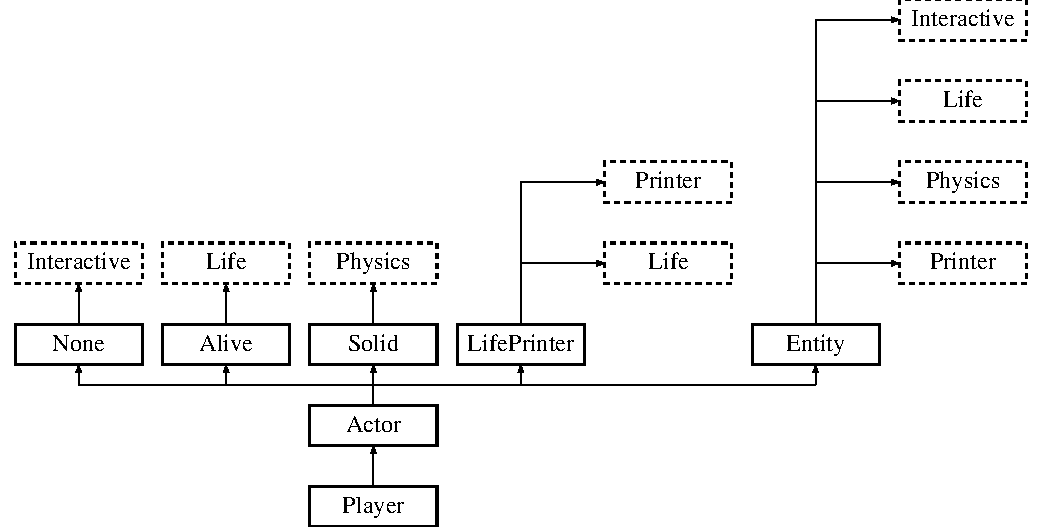
\includegraphics[height=7.000000cm]{class_player}
\end{center}
\end{figure}
\subsection*{Public Member Functions}
\begin{DoxyCompactItemize}
\item 
\hyperlink{class_player_ac9e3911538a0ce6b4bbae000671136bb}{Player} (unsigned int \hyperlink{class_entity_afa8f48eccdb09a290e2c1ded3f135363}{x}, unsigned \hyperlink{class_entity_a9d39843430829a89bb8233dbaadae4f1}{y}, std\-::string \-\_\-name)
\item 
void \hyperlink{class_player_a43124e562ec95ecd4a2aece053b65098}{info} (std\-::ostream \&out)
\end{DoxyCompactItemize}
\subsection*{Additional Inherited Members}


\subsection{Constructor \& Destructor Documentation}
\hypertarget{class_player_ac9e3911538a0ce6b4bbae000671136bb}{\index{Player@{Player}!Player@{Player}}
\index{Player@{Player}!Player@{Player}}
\subsubsection[{Player}]{\setlength{\rightskip}{0pt plus 5cm}Player\-::\-Player (
\begin{DoxyParamCaption}
\item[{unsigned int}]{x, }
\item[{unsigned}]{y, }
\item[{std\-::string}]{\-\_\-name}
\end{DoxyParamCaption}
)}}\label{class_player_ac9e3911538a0ce6b4bbae000671136bb}
E\-N\-S\-U\-R\-E(\hyperlink{class_entity_af7f20142aa7883ca29a91c43e3511e48}{properly\-Initialized()}, \char`\"{}\-Constructor must end...\char`\"{}) 

\subsection{Member Function Documentation}
\hypertarget{class_player_a43124e562ec95ecd4a2aece053b65098}{\index{Player@{Player}!info@{info}}
\index{info@{info}!Player@{Player}}
\subsubsection[{info}]{\setlength{\rightskip}{0pt plus 5cm}void Player\-::info (
\begin{DoxyParamCaption}
\item[{std\-::ostream \&}]{out}
\end{DoxyParamCaption}
)\hspace{0.3cm}{\ttfamily [virtual]}}}\label{class_player_a43124e562ec95ecd4a2aece053b65098}
R\-E\-Q\-U\-I\-R\-E(\hyperlink{class_entity_af7f20142aa7883ca29a91c43e3511e48}{properly\-Initialized()}, \char`\"{}\-Player wasn't initialized when calling info\char`\"{}) 

Implements \hyperlink{class_entity_aa694874d1f59971187de675d1e0c1fdf}{Entity}.



The documentation for this class was generated from the following files\-:\begin{DoxyCompactItemize}
\item 
entities/\hyperlink{player_8h}{player.\-h}\item 
entities/\hyperlink{player_8cpp}{player.\-cpp}\end{DoxyCompactItemize}

\hypertarget{class_printer}{\section{Printer Class Reference}
\label{class_printer}\index{Printer@{Printer}}
}


{\ttfamily \#include $<$printer.\-h$>$}

Inheritance diagram for Printer\-:\begin{figure}[H]
\begin{center}
\leavevmode
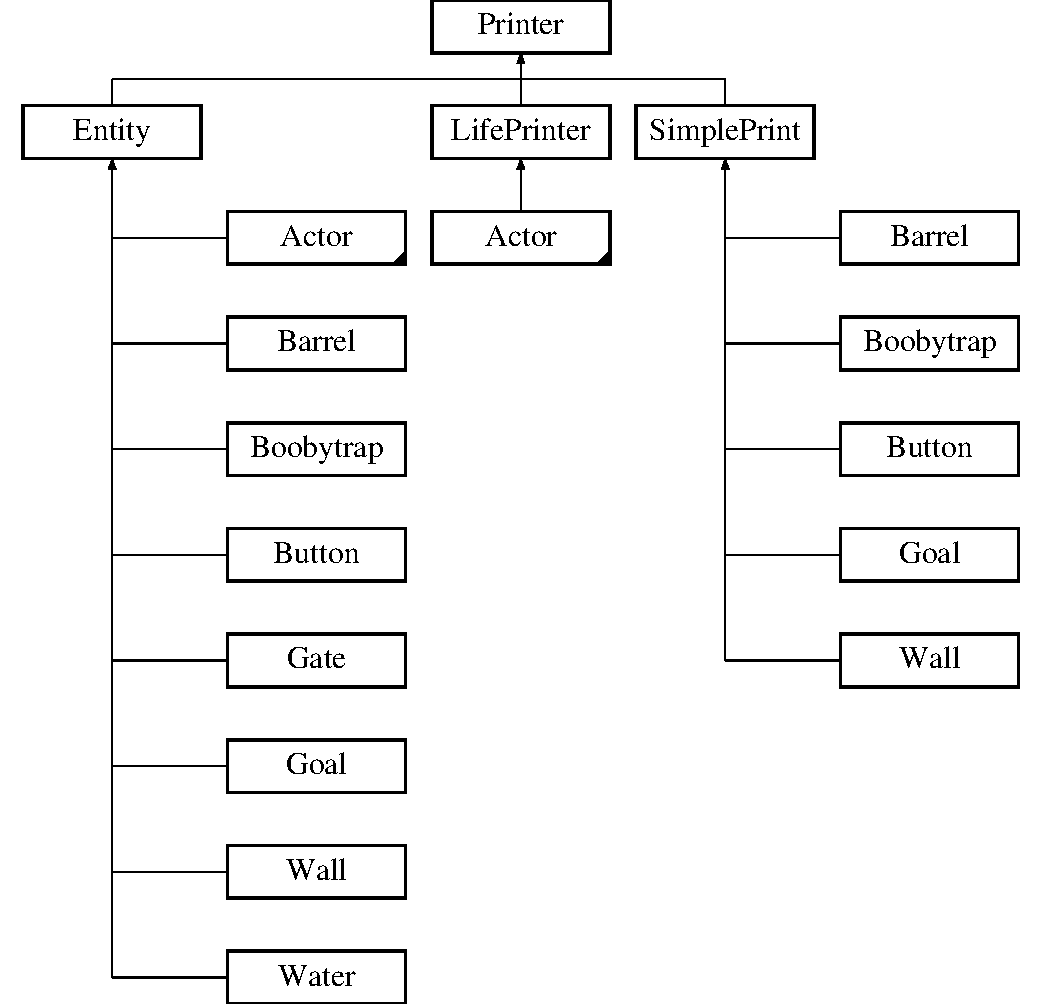
\includegraphics[height=10.000000cm]{class_printer}
\end{center}
\end{figure}
\subsection*{Public Member Functions}
\begin{DoxyCompactItemize}
\item 
virtual void \hyperlink{class_printer_ae92d7cb7cbb97d1427a352ce055c89f0}{\-\_\-\-\_\-polymorphic\-\_\-\-\_\-} ()
\item 
virtual char \hyperlink{class_printer_a66ecfd99bb8bc0a88ed0fc1276c70e23}{to\-\_\-char} ()=0
\item 
virtual \hyperlink{class_printer_ab537b50f5dfc65a74908db69c556d0f8}{$\sim$\-Printer} ()
\end{DoxyCompactItemize}


\subsection{Constructor \& Destructor Documentation}
\hypertarget{class_printer_ab537b50f5dfc65a74908db69c556d0f8}{\index{Printer@{Printer}!$\sim$\-Printer@{$\sim$\-Printer}}
\index{$\sim$\-Printer@{$\sim$\-Printer}!Printer@{Printer}}
\subsubsection[{$\sim$\-Printer}]{\setlength{\rightskip}{0pt plus 5cm}virtual Printer\-::$\sim$\-Printer (
\begin{DoxyParamCaption}
{}
\end{DoxyParamCaption}
)\hspace{0.3cm}{\ttfamily [inline]}, {\ttfamily [virtual]}}}\label{class_printer_ab537b50f5dfc65a74908db69c556d0f8}


\subsection{Member Function Documentation}
\hypertarget{class_printer_ae92d7cb7cbb97d1427a352ce055c89f0}{\index{Printer@{Printer}!\-\_\-\-\_\-polymorphic\-\_\-\-\_\-@{\-\_\-\-\_\-polymorphic\-\_\-\-\_\-}}
\index{\-\_\-\-\_\-polymorphic\-\_\-\-\_\-@{\-\_\-\-\_\-polymorphic\-\_\-\-\_\-}!Printer@{Printer}}
\subsubsection[{\-\_\-\-\_\-polymorphic\-\_\-\-\_\-}]{\setlength{\rightskip}{0pt plus 5cm}virtual void Printer\-::\-\_\-\-\_\-polymorphic\-\_\-\-\_\- (
\begin{DoxyParamCaption}
{}
\end{DoxyParamCaption}
)\hspace{0.3cm}{\ttfamily [inline]}, {\ttfamily [virtual]}}}\label{class_printer_ae92d7cb7cbb97d1427a352ce055c89f0}


Reimplemented in \hyperlink{class_entity_a11d5655c6e057fb86551402380009c01}{Entity}.

\hypertarget{class_printer_a66ecfd99bb8bc0a88ed0fc1276c70e23}{\index{Printer@{Printer}!to\-\_\-char@{to\-\_\-char}}
\index{to\-\_\-char@{to\-\_\-char}!Printer@{Printer}}
\subsubsection[{to\-\_\-char}]{\setlength{\rightskip}{0pt plus 5cm}virtual char Printer\-::to\-\_\-char (
\begin{DoxyParamCaption}
{}
\end{DoxyParamCaption}
)\hspace{0.3cm}{\ttfamily [pure virtual]}}}\label{class_printer_a66ecfd99bb8bc0a88ed0fc1276c70e23}


Implemented in \hyperlink{class_gate_a4c957d7092b0c53a0a8e711142818dfa}{Gate}, \hyperlink{class_water_a979406ad1fe514e132bf1d0e50802f49}{Water}, \hyperlink{class_life_printer_ab62c96990f0f0f605255e3394d64246b}{Life\-Printer}, and \hyperlink{class_simple_print_a96a054dd10cc1eb8b5139a8581b53c50}{Simple\-Print}.



The documentation for this class was generated from the following file\-:\begin{DoxyCompactItemize}
\item 
entities/printer/\hyperlink{printer_8h}{printer.\-h}\end{DoxyCompactItemize}

\hypertarget{classprecompile_1_1_rule}{\section{precompile.\-Rule Class Reference}
\label{classprecompile_1_1_rule}\index{precompile.\-Rule@{precompile.\-Rule}}
}
\subsection*{Public Member Functions}
\begin{DoxyCompactItemize}
\item 
def \hyperlink{classprecompile_1_1_rule_aa93d4e42de2fcd4fe853f4c6833311c4}{\-\_\-\-\_\-init\-\_\-\-\_\-}
\item 
def \hyperlink{classprecompile_1_1_rule_a1dcbe514ac5a84083102720b93dd144d}{call}
\item 
def \hyperlink{classprecompile_1_1_rule_a396e0bc608dd51e7fb92d722d3ad7c45}{get}
\end{DoxyCompactItemize}
\subsection*{Public Attributes}
\begin{DoxyCompactItemize}
\item 
\hyperlink{classprecompile_1_1_rule_ab0ff3b4766f25405312c0edb807a1fd0}{types}
\item 
\hyperlink{classprecompile_1_1_rule_abb65ba8d5e80deffd9124437cd2e25b1}{priority}
\end{DoxyCompactItemize}


\subsection{Constructor \& Destructor Documentation}
\hypertarget{classprecompile_1_1_rule_aa93d4e42de2fcd4fe853f4c6833311c4}{\index{precompile\-::\-Rule@{precompile\-::\-Rule}!\-\_\-\-\_\-init\-\_\-\-\_\-@{\-\_\-\-\_\-init\-\_\-\-\_\-}}
\index{\-\_\-\-\_\-init\-\_\-\-\_\-@{\-\_\-\-\_\-init\-\_\-\-\_\-}!precompile::Rule@{precompile\-::\-Rule}}
\subsubsection[{\-\_\-\-\_\-init\-\_\-\-\_\-}]{\setlength{\rightskip}{0pt plus 5cm}def precompile.\-Rule.\-\_\-\-\_\-init\-\_\-\-\_\- (
\begin{DoxyParamCaption}
\item[{}]{self, }
\item[{}]{types, }
\item[{}]{priority}
\end{DoxyParamCaption}
)}}\label{classprecompile_1_1_rule_aa93d4e42de2fcd4fe853f4c6833311c4}


\subsection{Member Function Documentation}
\hypertarget{classprecompile_1_1_rule_a1dcbe514ac5a84083102720b93dd144d}{\index{precompile\-::\-Rule@{precompile\-::\-Rule}!call@{call}}
\index{call@{call}!precompile::Rule@{precompile\-::\-Rule}}
\subsubsection[{call}]{\setlength{\rightskip}{0pt plus 5cm}def precompile.\-Rule.\-call (
\begin{DoxyParamCaption}
\item[{}]{self, }
\item[{}]{funcname, }
\item[{}]{varnames}
\end{DoxyParamCaption}
)}}\label{classprecompile_1_1_rule_a1dcbe514ac5a84083102720b93dd144d}
\hypertarget{classprecompile_1_1_rule_a396e0bc608dd51e7fb92d722d3ad7c45}{\index{precompile\-::\-Rule@{precompile\-::\-Rule}!get@{get}}
\index{get@{get}!precompile::Rule@{precompile\-::\-Rule}}
\subsubsection[{get}]{\setlength{\rightskip}{0pt plus 5cm}def precompile.\-Rule.\-get (
\begin{DoxyParamCaption}
\item[{}]{self, }
\item[{}]{args}
\end{DoxyParamCaption}
)}}\label{classprecompile_1_1_rule_a396e0bc608dd51e7fb92d722d3ad7c45}


\subsection{Member Data Documentation}
\hypertarget{classprecompile_1_1_rule_abb65ba8d5e80deffd9124437cd2e25b1}{\index{precompile\-::\-Rule@{precompile\-::\-Rule}!priority@{priority}}
\index{priority@{priority}!precompile::Rule@{precompile\-::\-Rule}}
\subsubsection[{priority}]{\setlength{\rightskip}{0pt plus 5cm}precompile.\-Rule.\-priority}}\label{classprecompile_1_1_rule_abb65ba8d5e80deffd9124437cd2e25b1}
\hypertarget{classprecompile_1_1_rule_ab0ff3b4766f25405312c0edb807a1fd0}{\index{precompile\-::\-Rule@{precompile\-::\-Rule}!types@{types}}
\index{types@{types}!precompile::Rule@{precompile\-::\-Rule}}
\subsubsection[{types}]{\setlength{\rightskip}{0pt plus 5cm}precompile.\-Rule.\-types}}\label{classprecompile_1_1_rule_ab0ff3b4766f25405312c0edb807a1fd0}


The documentation for this class was generated from the following file\-:\begin{DoxyCompactItemize}
\item 
events/dispatch/\hyperlink{precompile_8py}{precompile.\-py}\end{DoxyCompactItemize}

\hypertarget{class_simple_physics}{\section{Simple\-Physics Class Reference}
\label{class_simple_physics}\index{Simple\-Physics@{Simple\-Physics}}
}


{\ttfamily \#include $<$simplephysics.\-h$>$}

Inheritance diagram for Simple\-Physics\-:\begin{figure}[H]
\begin{center}
\leavevmode
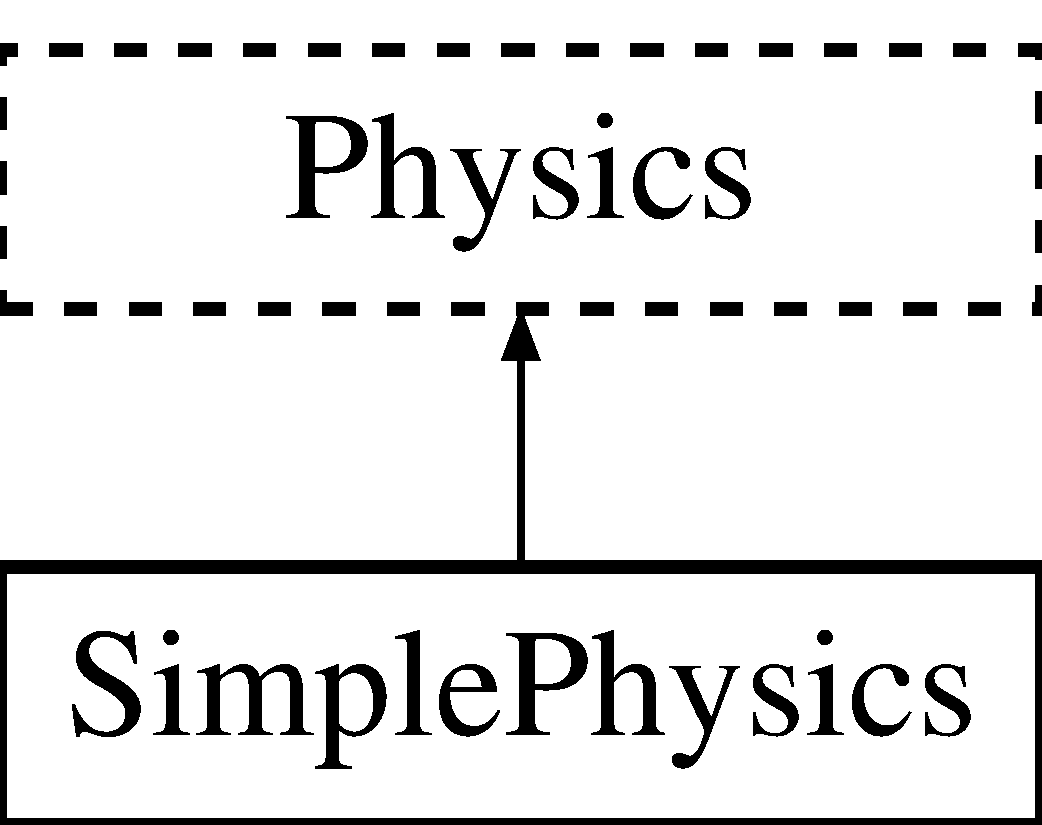
\includegraphics[height=2.000000cm]{class_simple_physics}
\end{center}
\end{figure}
\subsection*{Public Member Functions}
\begin{DoxyCompactItemize}
\item 
\hyperlink{class_simple_physics_a7b112689e7cbf3d4831a4cbcc5560156}{Simple\-Physics} (int \-\_\-height, int \-\_\-weight)
\item 
int \hyperlink{class_simple_physics_a28c8856df7f4abc5c483f6f1db2e8249}{get\-\_\-height} ()
\item 
int \hyperlink{class_simple_physics_a30837d444d7f3aee786546b25d075e58}{get\-\_\-weight} ()
\end{DoxyCompactItemize}


\subsection{Constructor \& Destructor Documentation}
\hypertarget{class_simple_physics_a7b112689e7cbf3d4831a4cbcc5560156}{\index{Simple\-Physics@{Simple\-Physics}!Simple\-Physics@{Simple\-Physics}}
\index{Simple\-Physics@{Simple\-Physics}!SimplePhysics@{Simple\-Physics}}
\subsubsection[{Simple\-Physics}]{\setlength{\rightskip}{0pt plus 5cm}Simple\-Physics\-::\-Simple\-Physics (
\begin{DoxyParamCaption}
\item[{int}]{\-\_\-height, }
\item[{int}]{\-\_\-weight}
\end{DoxyParamCaption}
)}}\label{class_simple_physics_a7b112689e7cbf3d4831a4cbcc5560156}


\subsection{Member Function Documentation}
\hypertarget{class_simple_physics_a28c8856df7f4abc5c483f6f1db2e8249}{\index{Simple\-Physics@{Simple\-Physics}!get\-\_\-height@{get\-\_\-height}}
\index{get\-\_\-height@{get\-\_\-height}!SimplePhysics@{Simple\-Physics}}
\subsubsection[{get\-\_\-height}]{\setlength{\rightskip}{0pt plus 5cm}int Simple\-Physics\-::get\-\_\-height (
\begin{DoxyParamCaption}
{}
\end{DoxyParamCaption}
)\hspace{0.3cm}{\ttfamily [virtual]}}}\label{class_simple_physics_a28c8856df7f4abc5c483f6f1db2e8249}


Implements \hyperlink{class_physics_ae3e59e7723c9f0334b88baf60c01f376}{Physics}.

\hypertarget{class_simple_physics_a30837d444d7f3aee786546b25d075e58}{\index{Simple\-Physics@{Simple\-Physics}!get\-\_\-weight@{get\-\_\-weight}}
\index{get\-\_\-weight@{get\-\_\-weight}!SimplePhysics@{Simple\-Physics}}
\subsubsection[{get\-\_\-weight}]{\setlength{\rightskip}{0pt plus 5cm}int Simple\-Physics\-::get\-\_\-weight (
\begin{DoxyParamCaption}
{}
\end{DoxyParamCaption}
)\hspace{0.3cm}{\ttfamily [virtual]}}}\label{class_simple_physics_a30837d444d7f3aee786546b25d075e58}


Implements \hyperlink{class_physics_a00580cf655d0569cc44f11b630cfcee7}{Physics}.



The documentation for this class was generated from the following files\-:\begin{DoxyCompactItemize}
\item 
entities/physics/\hyperlink{simplephysics_8h}{simplephysics.\-h}\item 
entities/physics/\hyperlink{simplephysics_8cpp}{simplephysics.\-cpp}\end{DoxyCompactItemize}

\hypertarget{class_simple_print}{\section{Simple\-Print Class Reference}
\label{class_simple_print}\index{Simple\-Print@{Simple\-Print}}
}


{\ttfamily \#include $<$simpleprint.\-h$>$}

Inheritance diagram for Simple\-Print\-:\begin{figure}[H]
\begin{center}
\leavevmode
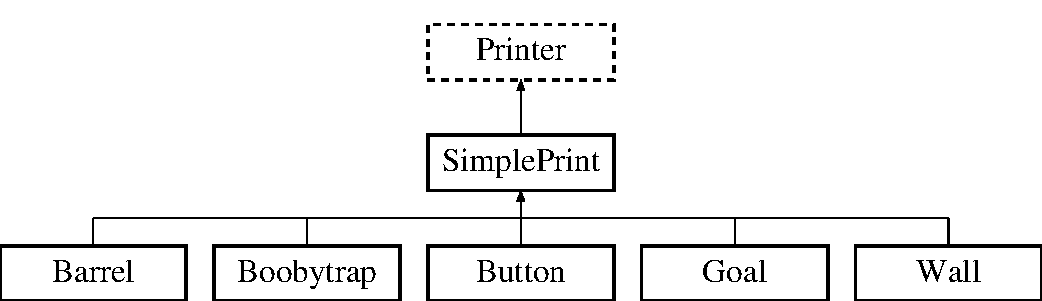
\includegraphics[height=3.000000cm]{class_simple_print}
\end{center}
\end{figure}
\subsection*{Public Member Functions}
\begin{DoxyCompactItemize}
\item 
\hyperlink{class_simple_print_ae02e09f4c1f2f4814654b07661294735}{Simple\-Print} (char s)
\item 
char \hyperlink{class_simple_print_a96a054dd10cc1eb8b5139a8581b53c50}{to\-\_\-char} ()
\end{DoxyCompactItemize}


\subsection{Constructor \& Destructor Documentation}
\hypertarget{class_simple_print_ae02e09f4c1f2f4814654b07661294735}{\index{Simple\-Print@{Simple\-Print}!Simple\-Print@{Simple\-Print}}
\index{Simple\-Print@{Simple\-Print}!SimplePrint@{Simple\-Print}}
\subsubsection[{Simple\-Print}]{\setlength{\rightskip}{0pt plus 5cm}Simple\-Print\-::\-Simple\-Print (
\begin{DoxyParamCaption}
\item[{char}]{s}
\end{DoxyParamCaption}
)}}\label{class_simple_print_ae02e09f4c1f2f4814654b07661294735}


\subsection{Member Function Documentation}
\hypertarget{class_simple_print_a96a054dd10cc1eb8b5139a8581b53c50}{\index{Simple\-Print@{Simple\-Print}!to\-\_\-char@{to\-\_\-char}}
\index{to\-\_\-char@{to\-\_\-char}!SimplePrint@{Simple\-Print}}
\subsubsection[{to\-\_\-char}]{\setlength{\rightskip}{0pt plus 5cm}char Simple\-Print\-::to\-\_\-char (
\begin{DoxyParamCaption}
{}
\end{DoxyParamCaption}
)\hspace{0.3cm}{\ttfamily [virtual]}}}\label{class_simple_print_a96a054dd10cc1eb8b5139a8581b53c50}


Implements \hyperlink{class_printer_a66ecfd99bb8bc0a88ed0fc1276c70e23}{Printer}.



The documentation for this class was generated from the following files\-:\begin{DoxyCompactItemize}
\item 
entities/printer/\hyperlink{simpleprint_8h}{simpleprint.\-h}\item 
entities/printer/\hyperlink{simpleprint_8cpp}{simpleprint.\-cpp}\end{DoxyCompactItemize}

\hypertarget{class_small}{\section{Small Class Reference}
\label{class_small}\index{Small@{Small}}
}


{\ttfamily \#include $<$small.\-h$>$}

Inheritance diagram for Small\-:\begin{figure}[H]
\begin{center}
\leavevmode
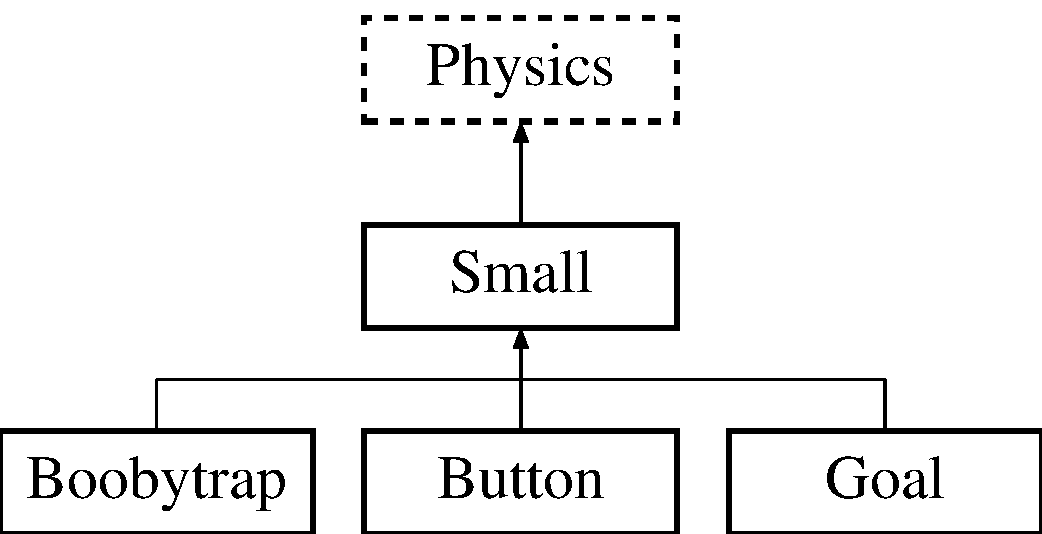
\includegraphics[height=3.000000cm]{class_small}
\end{center}
\end{figure}
\subsection*{Public Member Functions}
\begin{DoxyCompactItemize}
\item 
int \hyperlink{class_small_a89be5d71d35f47ad611670abda1b9cdf}{get\-\_\-height} ()
\item 
int \hyperlink{class_small_a088f55606741de6a39a7d9af5f78ada9}{get\-\_\-weight} ()
\end{DoxyCompactItemize}


\subsection{Member Function Documentation}
\hypertarget{class_small_a89be5d71d35f47ad611670abda1b9cdf}{\index{Small@{Small}!get\-\_\-height@{get\-\_\-height}}
\index{get\-\_\-height@{get\-\_\-height}!Small@{Small}}
\subsubsection[{get\-\_\-height}]{\setlength{\rightskip}{0pt plus 5cm}int Small\-::get\-\_\-height (
\begin{DoxyParamCaption}
{}
\end{DoxyParamCaption}
)\hspace{0.3cm}{\ttfamily [virtual]}}}\label{class_small_a89be5d71d35f47ad611670abda1b9cdf}


Implements \hyperlink{class_physics_ae3e59e7723c9f0334b88baf60c01f376}{Physics}.

\hypertarget{class_small_a088f55606741de6a39a7d9af5f78ada9}{\index{Small@{Small}!get\-\_\-weight@{get\-\_\-weight}}
\index{get\-\_\-weight@{get\-\_\-weight}!Small@{Small}}
\subsubsection[{get\-\_\-weight}]{\setlength{\rightskip}{0pt plus 5cm}int Small\-::get\-\_\-weight (
\begin{DoxyParamCaption}
{}
\end{DoxyParamCaption}
)\hspace{0.3cm}{\ttfamily [virtual]}}}\label{class_small_a088f55606741de6a39a7d9af5f78ada9}


Implements \hyperlink{class_physics_a00580cf655d0569cc44f11b630cfcee7}{Physics}.



The documentation for this class was generated from the following files\-:\begin{DoxyCompactItemize}
\item 
entities/physics/\hyperlink{small_8h}{small.\-h}\item 
entities/physics/\hyperlink{small_8cpp}{small.\-cpp}\end{DoxyCompactItemize}

\hypertarget{class_solid}{\section{Solid Class Reference}
\label{class_solid}\index{Solid@{Solid}}
}


{\ttfamily \#include $<$solid.\-h$>$}

Inheritance diagram for Solid\-:\begin{figure}[H]
\begin{center}
\leavevmode
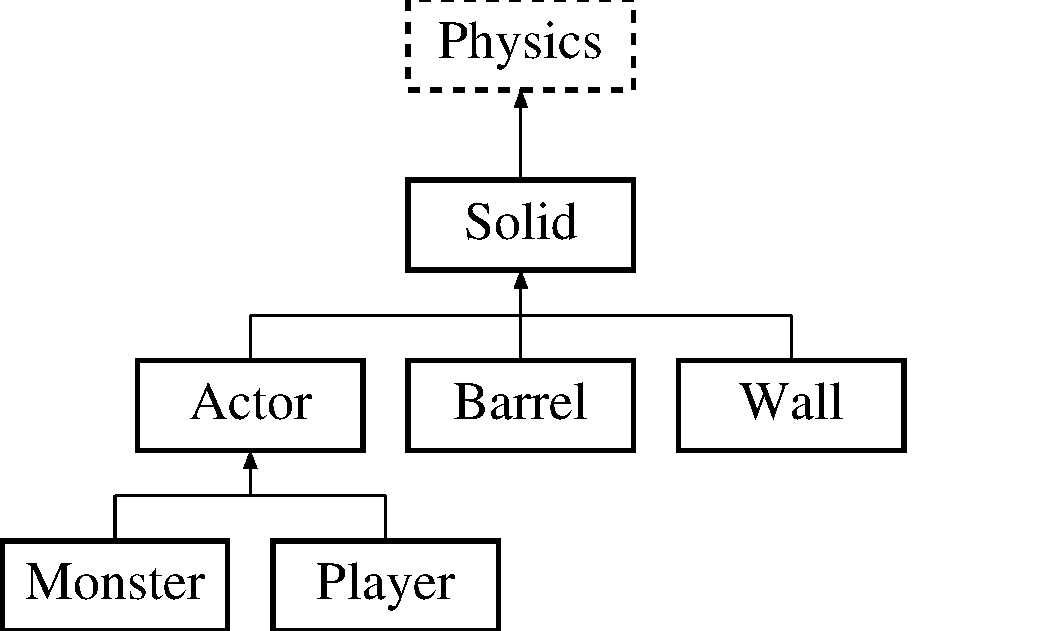
\includegraphics[height=4.000000cm]{class_solid}
\end{center}
\end{figure}
\subsection*{Public Member Functions}
\begin{DoxyCompactItemize}
\item 
\hyperlink{class_solid_a2f8cf8edb1bb73a0c0cd75082b80a28d}{Solid} (int \-\_\-height, int \-\_\-weight)
\item 
int \hyperlink{class_solid_a761885671b0a974a905c4056d7c8ef1f}{get\-\_\-height} ()
\item 
int \hyperlink{class_solid_a40e04cb5537a2f6f952fda357afbe970}{get\-\_\-weight} ()
\end{DoxyCompactItemize}


\subsection{Constructor \& Destructor Documentation}
\hypertarget{class_solid_a2f8cf8edb1bb73a0c0cd75082b80a28d}{\index{Solid@{Solid}!Solid@{Solid}}
\index{Solid@{Solid}!Solid@{Solid}}
\subsubsection[{Solid}]{\setlength{\rightskip}{0pt plus 5cm}Solid\-::\-Solid (
\begin{DoxyParamCaption}
\item[{int}]{\-\_\-height, }
\item[{int}]{\-\_\-weight}
\end{DoxyParamCaption}
)}}\label{class_solid_a2f8cf8edb1bb73a0c0cd75082b80a28d}


\subsection{Member Function Documentation}
\hypertarget{class_solid_a761885671b0a974a905c4056d7c8ef1f}{\index{Solid@{Solid}!get\-\_\-height@{get\-\_\-height}}
\index{get\-\_\-height@{get\-\_\-height}!Solid@{Solid}}
\subsubsection[{get\-\_\-height}]{\setlength{\rightskip}{0pt plus 5cm}int Solid\-::get\-\_\-height (
\begin{DoxyParamCaption}
{}
\end{DoxyParamCaption}
)\hspace{0.3cm}{\ttfamily [virtual]}}}\label{class_solid_a761885671b0a974a905c4056d7c8ef1f}


Implements \hyperlink{class_physics_ae3e59e7723c9f0334b88baf60c01f376}{Physics}.

\hypertarget{class_solid_a40e04cb5537a2f6f952fda357afbe970}{\index{Solid@{Solid}!get\-\_\-weight@{get\-\_\-weight}}
\index{get\-\_\-weight@{get\-\_\-weight}!Solid@{Solid}}
\subsubsection[{get\-\_\-weight}]{\setlength{\rightskip}{0pt plus 5cm}int Solid\-::get\-\_\-weight (
\begin{DoxyParamCaption}
{}
\end{DoxyParamCaption}
)\hspace{0.3cm}{\ttfamily [virtual]}}}\label{class_solid_a40e04cb5537a2f6f952fda357afbe970}


Implements \hyperlink{class_physics_a00580cf655d0569cc44f11b630cfcee7}{Physics}.



The documentation for this class was generated from the following files\-:\begin{DoxyCompactItemize}
\item 
entities/physics/\hyperlink{solid_8h}{solid.\-h}\item 
entities/physics/\hyperlink{solid_8cpp}{solid.\-cpp}\end{DoxyCompactItemize}

\hypertarget{class_symmetric_double_dispatcher}{\section{Symmetric\-Double\-Dispatcher$<$ Return\-T, Arg1\-T, Arg2\-T $>$ Class Template Reference}
\label{class_symmetric_double_dispatcher}\index{Symmetric\-Double\-Dispatcher$<$ Return\-T, Arg1\-T, Arg2\-T $>$@{Symmetric\-Double\-Dispatcher$<$ Return\-T, Arg1\-T, Arg2\-T $>$}}
}


{\ttfamily \#include $<$dispatch\-\_\-base.\-h$>$}

Inheritance diagram for Symmetric\-Double\-Dispatcher$<$ Return\-T, Arg1\-T, Arg2\-T $>$\-:\begin{figure}[H]
\begin{center}
\leavevmode
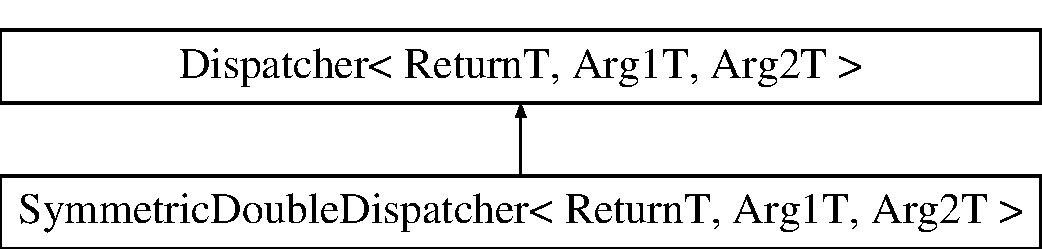
\includegraphics[height=2.000000cm]{class_symmetric_double_dispatcher}
\end{center}
\end{figure}
\subsection*{Public Member Functions}
\begin{DoxyCompactItemize}
\item 
Return\-T \hyperlink{class_symmetric_double_dispatcher_a05be0f4a0c041f56156525e18bc93f35}{operator()} (Arg1\-T arg1, Arg2\-T arg2)
\end{DoxyCompactItemize}


\subsection{Member Function Documentation}
\hypertarget{class_symmetric_double_dispatcher_a05be0f4a0c041f56156525e18bc93f35}{\index{Symmetric\-Double\-Dispatcher@{Symmetric\-Double\-Dispatcher}!operator()@{operator()}}
\index{operator()@{operator()}!SymmetricDoubleDispatcher@{Symmetric\-Double\-Dispatcher}}
\subsubsection[{operator()}]{\setlength{\rightskip}{0pt plus 5cm}template$<$typename Return\-T, typename Arg1\-T, typename Arg2\-T$>$ Return\-T {\bf Symmetric\-Double\-Dispatcher}$<$ Return\-T, Arg1\-T, Arg2\-T $>$\-::operator() (
\begin{DoxyParamCaption}
\item[{Arg1\-T}]{arg1, }
\item[{Arg2\-T}]{arg2}
\end{DoxyParamCaption}
)\hspace{0.3cm}{\ttfamily [inline]}}}\label{class_symmetric_double_dispatcher_a05be0f4a0c041f56156525e18bc93f35}


The documentation for this class was generated from the following file\-:\begin{DoxyCompactItemize}
\item 
events/dispatch/\hyperlink{dispatch__base_8h}{dispatch\-\_\-base.\-h}\end{DoxyCompactItemize}

\hypertarget{class_u_i}{\section{U\-I Class Reference}
\label{class_u_i}\index{U\-I@{U\-I}}
}


{\ttfamily \#include $<$U\-I.\-h$>$}

\subsection*{Public Member Functions}
\begin{DoxyCompactItemize}
\item 
\hyperlink{class_u_i_a675985a56b5e87ebdc8e5884b9f2ee09}{U\-I} ()
\item 
void \hyperlink{class_u_i_ae02d9a71dd29b037d1ee7d8bd673c1de}{reset} ()
\item 
void \hyperlink{class_u_i_a6bdaec41e41f67039516936fae3f0c30}{run} ()
\item 
void \hyperlink{class_u_i_a96b47da4488ec28a5cbb7eb31f332d72}{fancy\-\_\-command} (std\-::string \&command)
\item 
bool \hyperlink{class_u_i_aa40f2ee754e1bbf193f1661aeb6928bc}{parse\-\_\-and\-\_\-do} (std\-::string \&command)
\item 
void \hyperlink{class_u_i_a492a00f5cc27e21fab4bbd812fb6c4ee}{help} ()
\item 
void \hyperlink{class_u_i_aceecd424a608445e4ee9f4b8ee75a64b}{read\-\_\-board} (std\-::string \&filename)
\item 
void \hyperlink{class_u_i_a3036f1791dce9d55da94d4e572b0d4a3}{read\-\_\-actions} (std\-::string \&filename)
\item 
void \hyperlink{class_u_i_af69a6800f49eb64c616b9d3c6e861776}{simulate} ()
\item 
void \hyperlink{class_u_i_a622632c0a198b6d799489eff4f1069c3}{write\-\_\-board} (std\-::ostream \&out)
\item 
void \hyperlink{class_u_i_a96dcbe153fb0624e4695a32ea99233b4}{write\-\_\-actions} (std\-::ostream \&out)
\item 
void \hyperlink{class_u_i_a589a1aaee2f73707fef65872b1ba9853}{show} (std\-::ostream \&out)
\item 
bool \hyperlink{class_u_i_adf4e96404df921e04f60217c93763fcd}{init\-\_\-game} ()
\end{DoxyCompactItemize}


\subsection{Constructor \& Destructor Documentation}
\hypertarget{class_u_i_a675985a56b5e87ebdc8e5884b9f2ee09}{\index{U\-I@{U\-I}!U\-I@{U\-I}}
\index{U\-I@{U\-I}!UI@{U\-I}}
\subsubsection[{U\-I}]{\setlength{\rightskip}{0pt plus 5cm}U\-I\-::\-U\-I (
\begin{DoxyParamCaption}
{}
\end{DoxyParamCaption}
)}}\label{class_u_i_a675985a56b5e87ebdc8e5884b9f2ee09}


\subsection{Member Function Documentation}
\hypertarget{class_u_i_a96b47da4488ec28a5cbb7eb31f332d72}{\index{U\-I@{U\-I}!fancy\-\_\-command@{fancy\-\_\-command}}
\index{fancy\-\_\-command@{fancy\-\_\-command}!UI@{U\-I}}
\subsubsection[{fancy\-\_\-command}]{\setlength{\rightskip}{0pt plus 5cm}void U\-I\-::fancy\-\_\-command (
\begin{DoxyParamCaption}
\item[{std\-::string \&}]{command}
\end{DoxyParamCaption}
)}}\label{class_u_i_a96b47da4488ec28a5cbb7eb31f332d72}
\hypertarget{class_u_i_a492a00f5cc27e21fab4bbd812fb6c4ee}{\index{U\-I@{U\-I}!help@{help}}
\index{help@{help}!UI@{U\-I}}
\subsubsection[{help}]{\setlength{\rightskip}{0pt plus 5cm}void U\-I\-::help (
\begin{DoxyParamCaption}
{}
\end{DoxyParamCaption}
)}}\label{class_u_i_a492a00f5cc27e21fab4bbd812fb6c4ee}
\hypertarget{class_u_i_adf4e96404df921e04f60217c93763fcd}{\index{U\-I@{U\-I}!init\-\_\-game@{init\-\_\-game}}
\index{init\-\_\-game@{init\-\_\-game}!UI@{U\-I}}
\subsubsection[{init\-\_\-game}]{\setlength{\rightskip}{0pt plus 5cm}bool U\-I\-::init\-\_\-game (
\begin{DoxyParamCaption}
{}
\end{DoxyParamCaption}
)}}\label{class_u_i_adf4e96404df921e04f60217c93763fcd}
\hypertarget{class_u_i_aa40f2ee754e1bbf193f1661aeb6928bc}{\index{U\-I@{U\-I}!parse\-\_\-and\-\_\-do@{parse\-\_\-and\-\_\-do}}
\index{parse\-\_\-and\-\_\-do@{parse\-\_\-and\-\_\-do}!UI@{U\-I}}
\subsubsection[{parse\-\_\-and\-\_\-do}]{\setlength{\rightskip}{0pt plus 5cm}bool U\-I\-::parse\-\_\-and\-\_\-do (
\begin{DoxyParamCaption}
\item[{std\-::string \&}]{command}
\end{DoxyParamCaption}
)}}\label{class_u_i_aa40f2ee754e1bbf193f1661aeb6928bc}
\hypertarget{class_u_i_a3036f1791dce9d55da94d4e572b0d4a3}{\index{U\-I@{U\-I}!read\-\_\-actions@{read\-\_\-actions}}
\index{read\-\_\-actions@{read\-\_\-actions}!UI@{U\-I}}
\subsubsection[{read\-\_\-actions}]{\setlength{\rightskip}{0pt plus 5cm}void U\-I\-::read\-\_\-actions (
\begin{DoxyParamCaption}
\item[{std\-::string \&}]{filename}
\end{DoxyParamCaption}
)}}\label{class_u_i_a3036f1791dce9d55da94d4e572b0d4a3}
\hypertarget{class_u_i_aceecd424a608445e4ee9f4b8ee75a64b}{\index{U\-I@{U\-I}!read\-\_\-board@{read\-\_\-board}}
\index{read\-\_\-board@{read\-\_\-board}!UI@{U\-I}}
\subsubsection[{read\-\_\-board}]{\setlength{\rightskip}{0pt plus 5cm}void U\-I\-::read\-\_\-board (
\begin{DoxyParamCaption}
\item[{std\-::string \&}]{filename}
\end{DoxyParamCaption}
)}}\label{class_u_i_aceecd424a608445e4ee9f4b8ee75a64b}
\hypertarget{class_u_i_ae02d9a71dd29b037d1ee7d8bd673c1de}{\index{U\-I@{U\-I}!reset@{reset}}
\index{reset@{reset}!UI@{U\-I}}
\subsubsection[{reset}]{\setlength{\rightskip}{0pt plus 5cm}void U\-I\-::reset (
\begin{DoxyParamCaption}
{}
\end{DoxyParamCaption}
)}}\label{class_u_i_ae02d9a71dd29b037d1ee7d8bd673c1de}
\hypertarget{class_u_i_a6bdaec41e41f67039516936fae3f0c30}{\index{U\-I@{U\-I}!run@{run}}
\index{run@{run}!UI@{U\-I}}
\subsubsection[{run}]{\setlength{\rightskip}{0pt plus 5cm}void U\-I\-::run (
\begin{DoxyParamCaption}
{}
\end{DoxyParamCaption}
)}}\label{class_u_i_a6bdaec41e41f67039516936fae3f0c30}
\hypertarget{class_u_i_a589a1aaee2f73707fef65872b1ba9853}{\index{U\-I@{U\-I}!show@{show}}
\index{show@{show}!UI@{U\-I}}
\subsubsection[{show}]{\setlength{\rightskip}{0pt plus 5cm}void U\-I\-::show (
\begin{DoxyParamCaption}
\item[{std\-::ostream \&}]{out}
\end{DoxyParamCaption}
)}}\label{class_u_i_a589a1aaee2f73707fef65872b1ba9853}
\hypertarget{class_u_i_af69a6800f49eb64c616b9d3c6e861776}{\index{U\-I@{U\-I}!simulate@{simulate}}
\index{simulate@{simulate}!UI@{U\-I}}
\subsubsection[{simulate}]{\setlength{\rightskip}{0pt plus 5cm}void U\-I\-::simulate (
\begin{DoxyParamCaption}
{}
\end{DoxyParamCaption}
)}}\label{class_u_i_af69a6800f49eb64c616b9d3c6e861776}
\hypertarget{class_u_i_a96dcbe153fb0624e4695a32ea99233b4}{\index{U\-I@{U\-I}!write\-\_\-actions@{write\-\_\-actions}}
\index{write\-\_\-actions@{write\-\_\-actions}!UI@{U\-I}}
\subsubsection[{write\-\_\-actions}]{\setlength{\rightskip}{0pt plus 5cm}void U\-I\-::write\-\_\-actions (
\begin{DoxyParamCaption}
\item[{std\-::ostream \&}]{out}
\end{DoxyParamCaption}
)}}\label{class_u_i_a96dcbe153fb0624e4695a32ea99233b4}
\hypertarget{class_u_i_a622632c0a198b6d799489eff4f1069c3}{\index{U\-I@{U\-I}!write\-\_\-board@{write\-\_\-board}}
\index{write\-\_\-board@{write\-\_\-board}!UI@{U\-I}}
\subsubsection[{write\-\_\-board}]{\setlength{\rightskip}{0pt plus 5cm}void U\-I\-::write\-\_\-board (
\begin{DoxyParamCaption}
\item[{std\-::ostream \&}]{out}
\end{DoxyParamCaption}
)}}\label{class_u_i_a622632c0a198b6d799489eff4f1069c3}


The documentation for this class was generated from the following files\-:\begin{DoxyCompactItemize}
\item 
U\-I/\hyperlink{_u_i_8h}{U\-I.\-h}\item 
U\-I/\hyperlink{_u_i_8cpp}{U\-I.\-cpp}\end{DoxyCompactItemize}

\hypertarget{class_wall}{\section{Wall Class Reference}
\label{class_wall}\index{Wall@{Wall}}
}


{\ttfamily \#include $<$wall.\-h$>$}

Inheritance diagram for Wall\-:\begin{figure}[H]
\begin{center}
\leavevmode
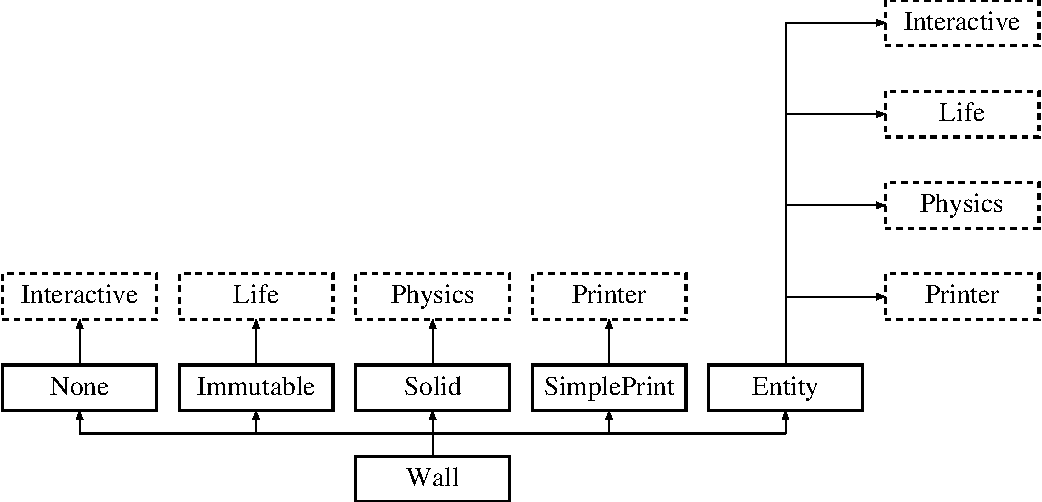
\includegraphics[height=6.000000cm]{class_wall}
\end{center}
\end{figure}
\subsection*{Public Member Functions}
\begin{DoxyCompactItemize}
\item 
\hyperlink{class_wall_a00ec988fcc89a3c1645b0d84c31f1613}{Wall} (unsigned int \hyperlink{class_entity_afa8f48eccdb09a290e2c1ded3f135363}{x}, unsigned \hyperlink{class_entity_a9d39843430829a89bb8233dbaadae4f1}{y})
\item 
void \hyperlink{class_wall_a0ff5e8bb39976f825e99dcd51a2ee610}{info} (std\-::ostream \&out)
\end{DoxyCompactItemize}
\subsection*{Additional Inherited Members}


\subsection{Constructor \& Destructor Documentation}
\hypertarget{class_wall_a00ec988fcc89a3c1645b0d84c31f1613}{\index{Wall@{Wall}!Wall@{Wall}}
\index{Wall@{Wall}!Wall@{Wall}}
\subsubsection[{Wall}]{\setlength{\rightskip}{0pt plus 5cm}Wall\-::\-Wall (
\begin{DoxyParamCaption}
\item[{unsigned int}]{x, }
\item[{unsigned}]{y}
\end{DoxyParamCaption}
)}}\label{class_wall_a00ec988fcc89a3c1645b0d84c31f1613}


\subsection{Member Function Documentation}
\hypertarget{class_wall_a0ff5e8bb39976f825e99dcd51a2ee610}{\index{Wall@{Wall}!info@{info}}
\index{info@{info}!Wall@{Wall}}
\subsubsection[{info}]{\setlength{\rightskip}{0pt plus 5cm}void Wall\-::info (
\begin{DoxyParamCaption}
\item[{std\-::ostream \&}]{out}
\end{DoxyParamCaption}
)\hspace{0.3cm}{\ttfamily [virtual]}}}\label{class_wall_a0ff5e8bb39976f825e99dcd51a2ee610}
Shows the info about the entity, used in the method \hyperlink{class_board_ae7e407126c1c113669e645a216fc7848}{Board\-::write\-\_\-board}. Is a pure virtual function for \hyperlink{class_entity}{Entity}. R\-E\-Q\-U\-I\-R\-E(\hyperlink{class_entity_af7f20142aa7883ca29a91c43e3511e48}{properly\-Initialized()}, \char`\"{}\-Entity wasn't initialized when calling info\char`\"{}) 

Implements \hyperlink{class_entity_aa694874d1f59971187de675d1e0c1fdf}{Entity}.



The documentation for this class was generated from the following files\-:\begin{DoxyCompactItemize}
\item 
entities/\hyperlink{wall_8h}{wall.\-h}\item 
entities/\hyperlink{wall_8cpp}{wall.\-cpp}\end{DoxyCompactItemize}

\hypertarget{class_water}{\section{Water Class Reference}
\label{class_water}\index{Water@{Water}}
}


{\ttfamily \#include $<$water.\-h$>$}

Inheritance diagram for Water\-:\begin{figure}[H]
\begin{center}
\leavevmode
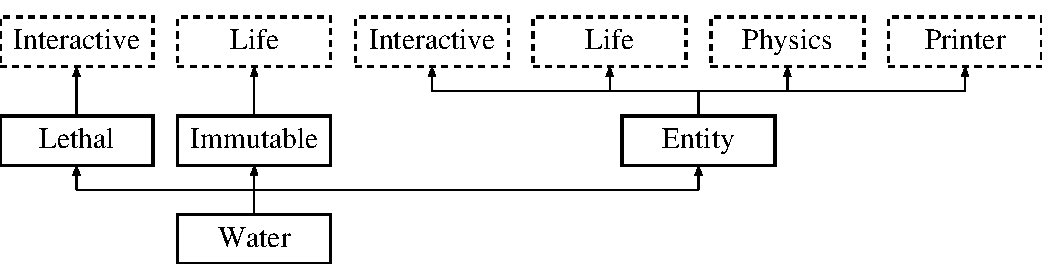
\includegraphics[height=3.000000cm]{class_water}
\end{center}
\end{figure}
\subsection*{Public Member Functions}
\begin{DoxyCompactItemize}
\item 
\hyperlink{class_water_ab5347dafc5898a03fd556f1640d0fd55}{Water} (unsigned int \hyperlink{class_entity_afa8f48eccdb09a290e2c1ded3f135363}{x}, unsigned \hyperlink{class_entity_a9d39843430829a89bb8233dbaadae4f1}{y})
\item 
bool \hyperlink{class_water_a063397ad0da6b286bdad0a27cc646cb4}{is\-\_\-filled} ()
\item 
char \hyperlink{class_water_a979406ad1fe514e132bf1d0e50802f49}{to\-\_\-char} ()
\item 
int \hyperlink{class_water_a3f9cea082bd0a91d0e8a3b5737d3fbd2}{get\-\_\-weight} ()
\item 
int \hyperlink{class_water_a090400fa44c929081aa6b097ed6f16e7}{get\-\_\-height} ()
\item 
void \hyperlink{class_water_a0931381448954bfc525aa6492860f599}{info} (std\-::ostream \&out)
\end{DoxyCompactItemize}
\subsection*{Public Attributes}
\begin{DoxyCompactItemize}
\item 
\hyperlink{class_entity}{Entity} $\ast$ \hyperlink{class_water_a71b18a4a6cbd58ebbe7c927a84eaab3c}{contained}
\end{DoxyCompactItemize}


\subsection{Constructor \& Destructor Documentation}
\hypertarget{class_water_ab5347dafc5898a03fd556f1640d0fd55}{\index{Water@{Water}!Water@{Water}}
\index{Water@{Water}!Water@{Water}}
\subsubsection[{Water}]{\setlength{\rightskip}{0pt plus 5cm}Water\-::\-Water (
\begin{DoxyParamCaption}
\item[{unsigned int}]{x, }
\item[{unsigned}]{y}
\end{DoxyParamCaption}
)}}\label{class_water_ab5347dafc5898a03fd556f1640d0fd55}


\subsection{Member Function Documentation}
\hypertarget{class_water_a090400fa44c929081aa6b097ed6f16e7}{\index{Water@{Water}!get\-\_\-height@{get\-\_\-height}}
\index{get\-\_\-height@{get\-\_\-height}!Water@{Water}}
\subsubsection[{get\-\_\-height}]{\setlength{\rightskip}{0pt plus 5cm}int Water\-::get\-\_\-height (
\begin{DoxyParamCaption}
{}
\end{DoxyParamCaption}
)\hspace{0.3cm}{\ttfamily [virtual]}}}\label{class_water_a090400fa44c929081aa6b097ed6f16e7}


Implements \hyperlink{class_physics_ae3e59e7723c9f0334b88baf60c01f376}{Physics}.

\hypertarget{class_water_a3f9cea082bd0a91d0e8a3b5737d3fbd2}{\index{Water@{Water}!get\-\_\-weight@{get\-\_\-weight}}
\index{get\-\_\-weight@{get\-\_\-weight}!Water@{Water}}
\subsubsection[{get\-\_\-weight}]{\setlength{\rightskip}{0pt plus 5cm}int Water\-::get\-\_\-weight (
\begin{DoxyParamCaption}
{}
\end{DoxyParamCaption}
)\hspace{0.3cm}{\ttfamily [virtual]}}}\label{class_water_a3f9cea082bd0a91d0e8a3b5737d3fbd2}


Implements \hyperlink{class_physics_a00580cf655d0569cc44f11b630cfcee7}{Physics}.

\hypertarget{class_water_a0931381448954bfc525aa6492860f599}{\index{Water@{Water}!info@{info}}
\index{info@{info}!Water@{Water}}
\subsubsection[{info}]{\setlength{\rightskip}{0pt plus 5cm}void Water\-::info (
\begin{DoxyParamCaption}
\item[{std\-::ostream \&}]{out}
\end{DoxyParamCaption}
)\hspace{0.3cm}{\ttfamily [virtual]}}}\label{class_water_a0931381448954bfc525aa6492860f599}
Shows the info about the entity, used in the method \hyperlink{class_board_ae7e407126c1c113669e645a216fc7848}{Board\-::write\-\_\-board}. Is a pure virtual function for \hyperlink{class_entity}{Entity}. R\-E\-Q\-U\-I\-R\-E(\hyperlink{class_entity_af7f20142aa7883ca29a91c43e3511e48}{properly\-Initialized()}, \char`\"{}\-Entity wasn't initialized when calling info\char`\"{}) 

Implements \hyperlink{class_entity_aa694874d1f59971187de675d1e0c1fdf}{Entity}.

\hypertarget{class_water_a063397ad0da6b286bdad0a27cc646cb4}{\index{Water@{Water}!is\-\_\-filled@{is\-\_\-filled}}
\index{is\-\_\-filled@{is\-\_\-filled}!Water@{Water}}
\subsubsection[{is\-\_\-filled}]{\setlength{\rightskip}{0pt plus 5cm}bool Water\-::is\-\_\-filled (
\begin{DoxyParamCaption}
{}
\end{DoxyParamCaption}
)}}\label{class_water_a063397ad0da6b286bdad0a27cc646cb4}
\hypertarget{class_water_a979406ad1fe514e132bf1d0e50802f49}{\index{Water@{Water}!to\-\_\-char@{to\-\_\-char}}
\index{to\-\_\-char@{to\-\_\-char}!Water@{Water}}
\subsubsection[{to\-\_\-char}]{\setlength{\rightskip}{0pt plus 5cm}char Water\-::to\-\_\-char (
\begin{DoxyParamCaption}
{}
\end{DoxyParamCaption}
)\hspace{0.3cm}{\ttfamily [virtual]}}}\label{class_water_a979406ad1fe514e132bf1d0e50802f49}


Implements \hyperlink{class_printer_a66ecfd99bb8bc0a88ed0fc1276c70e23}{Printer}.



\subsection{Member Data Documentation}
\hypertarget{class_water_a71b18a4a6cbd58ebbe7c927a84eaab3c}{\index{Water@{Water}!contained@{contained}}
\index{contained@{contained}!Water@{Water}}
\subsubsection[{contained}]{\setlength{\rightskip}{0pt plus 5cm}{\bf Entity}$\ast$ Water\-::contained}}\label{class_water_a71b18a4a6cbd58ebbe7c927a84eaab3c}


The documentation for this class was generated from the following files\-:\begin{DoxyCompactItemize}
\item 
entities/\hyperlink{water_8h}{water.\-h}\item 
entities/\hyperlink{water_8cpp}{water.\-cpp}\end{DoxyCompactItemize}

\chapter{File Documentation}
\hypertarget{actions_8cpp}{\section{actions/actions.cpp File Reference}
\label{actions_8cpp}\index{actions/actions.\-cpp@{actions/actions.\-cpp}}
}
{\ttfamily \#include \char`\"{}actions.\-h\char`\"{}}\\*
{\ttfamily \#include \char`\"{}game.\-h\char`\"{}}\\*
\subsection*{Functions}
\begin{DoxyCompactItemize}
\item 
std\-::ostream \& \hyperlink{actions_8cpp_a81c17e954a272036ec685b1e79b1b006}{operator$<$$<$} (std\-::ostream \&out, \hyperlink{class_direction}{Direction} \&d)
\end{DoxyCompactItemize}


\subsection{Function Documentation}
\hypertarget{actions_8cpp_a81c17e954a272036ec685b1e79b1b006}{\index{actions.\-cpp@{actions.\-cpp}!operator$<$$<$@{operator$<$$<$}}
\index{operator$<$$<$@{operator$<$$<$}!actions.cpp@{actions.\-cpp}}
\subsubsection[{operator$<$$<$}]{\setlength{\rightskip}{0pt plus 5cm}std\-::ostream\& operator$<$$<$ (
\begin{DoxyParamCaption}
\item[{std\-::ostream \&}]{out, }
\item[{{\bf Direction} \&}]{d}
\end{DoxyParamCaption}
)}}\label{actions_8cpp_a81c17e954a272036ec685b1e79b1b006}

\hypertarget{actions_8h}{\section{actions/actions.h File Reference}
\label{actions_8h}\index{actions/actions.\-h@{actions/actions.\-h}}
}
{\ttfamily \#include $<$iostream$>$}\\*
{\ttfamily \#include \char`\"{}../entities/actor.\-h\char`\"{}}\\*
{\ttfamily \#include \char`\"{}../entities/player.\-h\char`\"{}}\\*
{\ttfamily \#include $<$../entities/monster.\-h$>$}\\*
{\ttfamily \#include \char`\"{}string\char`\"{}}\\*
\subsection*{Classes}
\begin{DoxyCompactItemize}
\item 
class \hyperlink{class_direction}{Direction}
\item 
class \hyperlink{class_action}{Action}
\end{DoxyCompactItemize}

\hypertarget{attack_8cpp}{\section{actions/attack.cpp File Reference}
\label{attack_8cpp}\index{actions/attack.\-cpp@{actions/attack.\-cpp}}
}
{\ttfamily \#include \char`\"{}attack.\-h\char`\"{}}\\*
{\ttfamily \#include \char`\"{}game.\-h\char`\"{}}\\*
{\ttfamily \#include $<$iostream$>$}\\*

\hypertarget{attack_8h}{\section{actions/attack.h File Reference}
\label{attack_8h}\index{actions/attack.\-h@{actions/attack.\-h}}
}
{\ttfamily \#include \char`\"{}actions.\-h\char`\"{}}\\*
\subsection*{Classes}
\begin{DoxyCompactItemize}
\item 
class \hyperlink{class_attack}{Attack}
\end{DoxyCompactItemize}

\hypertarget{move_8cpp}{\section{actions/move.cpp File Reference}
\label{move_8cpp}\index{actions/move.\-cpp@{actions/move.\-cpp}}
}
{\ttfamily \#include \char`\"{}move.\-h\char`\"{}}\\*
{\ttfamily \#include \char`\"{}../game/game.\-h\char`\"{}}\\*
{\ttfamily \#include \char`\"{}../entities/constants.\-h\char`\"{}}\\*
{\ttfamily \#include \char`\"{}../entities/actor.\-h\char`\"{}}\\*
{\ttfamily \#include $<$iostream$>$}\\*

\hypertarget{move_8h}{\section{actions/move.h File Reference}
\label{move_8h}\index{actions/move.\-h@{actions/move.\-h}}
}
{\ttfamily \#include \char`\"{}actions.\-h\char`\"{}}\\*
\subsection*{Classes}
\begin{DoxyCompactItemize}
\item 
class \hyperlink{class_move}{Move}
\end{DoxyCompactItemize}

\hypertarget{_arcade_main_8cpp}{\section{Arcade\-Main.\-cpp File Reference}
\label{_arcade_main_8cpp}\index{Arcade\-Main.\-cpp@{Arcade\-Main.\-cpp}}
}
{\ttfamily \#include $<$iostream$>$}\\*
{\ttfamily \#include $<$functional$>$}\\*
{\ttfamily \#include \char`\"{}game/game.\-h\char`\"{}}\\*
{\ttfamily \#include \char`\"{}parsers/game\-\_\-parser.\-h\char`\"{}}\\*
{\ttfamily \#include \char`\"{}U\-I/\-U\-I.\-h\char`\"{}}\\*
{\ttfamily \#include \char`\"{}lib/tinyxml/tinyxml.\-h\char`\"{}}\\*
\subsection*{Functions}
\begin{DoxyCompactItemize}
\item 
int \hyperlink{_arcade_main_8cpp_a217dbf8b442f20279ea00b898af96f52}{main} (int argc, const char $\ast$$\ast$argv)
\end{DoxyCompactItemize}


\subsection{Function Documentation}
\hypertarget{_arcade_main_8cpp_a217dbf8b442f20279ea00b898af96f52}{\index{Arcade\-Main.\-cpp@{Arcade\-Main.\-cpp}!main@{main}}
\index{main@{main}!ArcadeMain.cpp@{Arcade\-Main.\-cpp}}
\subsubsection[{main}]{\setlength{\rightskip}{0pt plus 5cm}int main (
\begin{DoxyParamCaption}
\item[{int}]{argc, }
\item[{const char $\ast$$\ast$}]{argv}
\end{DoxyParamCaption}
)}}\label{_arcade_main_8cpp_a217dbf8b442f20279ea00b898af96f52}

\hypertarget{_arcade_tests_8cpp}{\section{Arcade\-Tests.\-cpp File Reference}
\label{_arcade_tests_8cpp}\index{Arcade\-Tests.\-cpp@{Arcade\-Tests.\-cpp}}
}
{\ttfamily \#include \char`\"{}gtest/gtest.\-h\char`\"{}}\\*
{\ttfamily \#include \char`\"{}game.\-h\char`\"{}}\\*
{\ttfamily \#include \char`\"{}../parsers/game\-\_\-parser.\-h\char`\"{}}\\*
{\ttfamily \#include $<$iostream$>$}\\*
{\ttfamily \#include $<$fstream$>$}\\*
{\ttfamily \#include $<$sys/stat.\-h$>$}\\*
{\ttfamily \#include \char`\"{}../lib/tinyxml/tinyxml.\-h\char`\"{}}\\*
{\ttfamily \#include \char`\"{}tests/filetests.\-tests\char`\"{}}\\*
{\ttfamily \#include \char`\"{}tests/etc.\-cpp\char`\"{}}\\*
\subsection*{Functions}
\begin{DoxyCompactItemize}
\item 
bool \hyperlink{_arcade_tests_8cpp_a5dc15d7dfd3cc647491dc46e297cf40b}{file\-Compare} (std\-::string left\-File\-Name, std\-::string right\-File\-Name)
\item 
\hyperlink{_arcade_tests_8cpp_a2eac4f8cc81fe10fdb5d6cf25485ac7d}{T\-E\-S\-T} (Meta, G\-Test\-Test)
\item 
int \hyperlink{_arcade_tests_8cpp_a3c04138a5bfe5d72780bb7e82a18e627}{main} (int argc, char $\ast$$\ast$argv)
\end{DoxyCompactItemize}


\subsection{Function Documentation}
\hypertarget{_arcade_tests_8cpp_a5dc15d7dfd3cc647491dc46e297cf40b}{\index{Arcade\-Tests.\-cpp@{Arcade\-Tests.\-cpp}!file\-Compare@{file\-Compare}}
\index{file\-Compare@{file\-Compare}!ArcadeTests.cpp@{Arcade\-Tests.\-cpp}}
\subsubsection[{file\-Compare}]{\setlength{\rightskip}{0pt plus 5cm}bool file\-Compare (
\begin{DoxyParamCaption}
\item[{std\-::string}]{left\-File\-Name, }
\item[{std\-::string}]{right\-File\-Name}
\end{DoxyParamCaption}
)}}\label{_arcade_tests_8cpp_a5dc15d7dfd3cc647491dc46e297cf40b}
Auxiliary function for file manipulation in unit tests. \hypertarget{_arcade_tests_8cpp_a3c04138a5bfe5d72780bb7e82a18e627}{\index{Arcade\-Tests.\-cpp@{Arcade\-Tests.\-cpp}!main@{main}}
\index{main@{main}!ArcadeTests.cpp@{Arcade\-Tests.\-cpp}}
\subsubsection[{main}]{\setlength{\rightskip}{0pt plus 5cm}int main (
\begin{DoxyParamCaption}
\item[{int}]{argc, }
\item[{char $\ast$$\ast$}]{argv}
\end{DoxyParamCaption}
)}}\label{_arcade_tests_8cpp_a3c04138a5bfe5d72780bb7e82a18e627}
\hypertarget{_arcade_tests_8cpp_a2eac4f8cc81fe10fdb5d6cf25485ac7d}{\index{Arcade\-Tests.\-cpp@{Arcade\-Tests.\-cpp}!T\-E\-S\-T@{T\-E\-S\-T}}
\index{T\-E\-S\-T@{T\-E\-S\-T}!ArcadeTests.cpp@{Arcade\-Tests.\-cpp}}
\subsubsection[{T\-E\-S\-T}]{\setlength{\rightskip}{0pt plus 5cm}T\-E\-S\-T (
\begin{DoxyParamCaption}
\item[{Meta}]{, }
\item[{G\-Test\-Test}]{}
\end{DoxyParamCaption}
)}}\label{_arcade_tests_8cpp_a2eac4f8cc81fe10fdb5d6cf25485ac7d}

\hypertarget{_design_by_contract_8h}{\section{Design\-By\-Contract.\-h File Reference}
\label{_design_by_contract_8h}\index{Design\-By\-Contract.\-h@{Design\-By\-Contract.\-h}}
}
{\ttfamily \#include $<$assert.\-h$>$}\\*
\subsection*{Macros}
\begin{DoxyCompactItemize}
\item 
\#define \hyperlink{_design_by_contract_8h_aeb774672b46dbe80afc14e0d1970f017}{R\-E\-Q\-U\-I\-R\-E}(assertion, what)~if (!(assertion)) \-\_\-\-\_\-assert (what, \-\_\-\-\_\-\-F\-I\-L\-E\-\_\-\-\_\-, \-\_\-\-\_\-\-L\-I\-N\-E\-\_\-\-\_\-)
\item 
\#define \hyperlink{_design_by_contract_8h_ab8da60ea2bcdd55183cc29d8526e6857}{E\-N\-S\-U\-R\-E}(assertion, what)~if (!(assertion)) \-\_\-\-\_\-assert (what, \-\_\-\-\_\-\-F\-I\-L\-E\-\_\-\-\_\-, \-\_\-\-\_\-\-L\-I\-N\-E\-\_\-\-\_\-)
\end{DoxyCompactItemize}


\subsection{Macro Definition Documentation}
\hypertarget{_design_by_contract_8h_ab8da60ea2bcdd55183cc29d8526e6857}{\index{Design\-By\-Contract.\-h@{Design\-By\-Contract.\-h}!E\-N\-S\-U\-R\-E@{E\-N\-S\-U\-R\-E}}
\index{E\-N\-S\-U\-R\-E@{E\-N\-S\-U\-R\-E}!DesignByContract.h@{Design\-By\-Contract.\-h}}
\subsubsection[{E\-N\-S\-U\-R\-E}]{\setlength{\rightskip}{0pt plus 5cm}\#define E\-N\-S\-U\-R\-E(
\begin{DoxyParamCaption}
\item[{}]{assertion, }
\item[{}]{what}
\end{DoxyParamCaption}
)~if (!(assertion)) \-\_\-\-\_\-assert (what, \-\_\-\-\_\-\-F\-I\-L\-E\-\_\-\-\_\-, \-\_\-\-\_\-\-L\-I\-N\-E\-\_\-\-\_\-)}}\label{_design_by_contract_8h_ab8da60ea2bcdd55183cc29d8526e6857}
\hypertarget{_design_by_contract_8h_aeb774672b46dbe80afc14e0d1970f017}{\index{Design\-By\-Contract.\-h@{Design\-By\-Contract.\-h}!R\-E\-Q\-U\-I\-R\-E@{R\-E\-Q\-U\-I\-R\-E}}
\index{R\-E\-Q\-U\-I\-R\-E@{R\-E\-Q\-U\-I\-R\-E}!DesignByContract.h@{Design\-By\-Contract.\-h}}
\subsubsection[{R\-E\-Q\-U\-I\-R\-E}]{\setlength{\rightskip}{0pt plus 5cm}\#define R\-E\-Q\-U\-I\-R\-E(
\begin{DoxyParamCaption}
\item[{}]{assertion, }
\item[{}]{what}
\end{DoxyParamCaption}
)~if (!(assertion)) \-\_\-\-\_\-assert (what, \-\_\-\-\_\-\-F\-I\-L\-E\-\_\-\-\_\-, \-\_\-\-\_\-\-L\-I\-N\-E\-\_\-\-\_\-)}}\label{_design_by_contract_8h_aeb774672b46dbe80afc14e0d1970f017}

\hypertarget{actor_8cpp}{\section{entities/actor.cpp File Reference}
\label{actor_8cpp}\index{entities/actor.\-cpp@{entities/actor.\-cpp}}
}
{\ttfamily \#include \char`\"{}actor.\-h\char`\"{}}\\*
{\ttfamily \#include \char`\"{}constants.\-h\char`\"{}}\\*

\hypertarget{actor_8h}{\section{entities/actor.h File Reference}
\label{actor_8h}\index{entities/actor.\-h@{entities/actor.\-h}}
}
{\ttfamily \#include $<$string$>$}\\*
{\ttfamily \#include \char`\"{}ia/none.\-h\char`\"{}}\\*
{\ttfamily \#include \char`\"{}life/alive.\-h\char`\"{}}\\*
{\ttfamily \#include \char`\"{}physics/solid.\-h\char`\"{}}\\*
{\ttfamily \#include \char`\"{}printer/lifeprinter.\-h\char`\"{}}\\*
{\ttfamily \#include \char`\"{}entity.\-h\char`\"{}}\\*
\subsection*{Classes}
\begin{DoxyCompactItemize}
\item 
class \hyperlink{class_actor}{Actor}
\end{DoxyCompactItemize}

\hypertarget{barrel_8cpp}{\section{entities/barrel.cpp File Reference}
\label{barrel_8cpp}\index{entities/barrel.\-cpp@{entities/barrel.\-cpp}}
}
{\ttfamily \#include \char`\"{}barrel.\-h\char`\"{}}\\*
{\ttfamily \#include \char`\"{}constants.\-h\char`\"{}}\\*

\hypertarget{barrel_8h}{\section{entities/barrel.h File Reference}
\label{barrel_8h}\index{entities/barrel.\-h@{entities/barrel.\-h}}
}
{\ttfamily \#include \char`\"{}entity.\-h\char`\"{}}\\*
{\ttfamily \#include \char`\"{}life/immutable.\-h\char`\"{}}\\*
{\ttfamily \#include \char`\"{}physics/solid.\-h\char`\"{}}\\*
{\ttfamily \#include \char`\"{}printer/simpleprint.\-h\char`\"{}}\\*
{\ttfamily \#include \char`\"{}ia/none.\-h\char`\"{}}\\*
\subsection*{Classes}
\begin{DoxyCompactItemize}
\item 
class \hyperlink{class_barrel}{Barrel}
\end{DoxyCompactItemize}

\hypertarget{boobytrap_8cpp}{\section{entities/boobytrap.cpp File Reference}
\label{boobytrap_8cpp}\index{entities/boobytrap.\-cpp@{entities/boobytrap.\-cpp}}
}
{\ttfamily \#include \char`\"{}boobytrap.\-h\char`\"{}}\\*
{\ttfamily \#include \char`\"{}constants.\-h\char`\"{}}\\*

\hypertarget{boobytrap_8h}{\section{entities/boobytrap.h File Reference}
\label{boobytrap_8h}\index{entities/boobytrap.\-h@{entities/boobytrap.\-h}}
}
{\ttfamily \#include \char`\"{}entity.\-h\char`\"{}}\\*
{\ttfamily \#include \char`\"{}life/alive.\-h\char`\"{}}\\*
{\ttfamily \#include \char`\"{}physics/small.\-h\char`\"{}}\\*
{\ttfamily \#include \char`\"{}printer/simpleprint.\-h\char`\"{}}\\*
{\ttfamily \#include \char`\"{}ia/none.\-h\char`\"{}}\\*
\subsection*{Classes}
\begin{DoxyCompactItemize}
\item 
class \hyperlink{class_boobytrap}{Boobytrap}
\end{DoxyCompactItemize}

\hypertarget{button_8cpp}{\section{entities/button.cpp File Reference}
\label{button_8cpp}\index{entities/button.\-cpp@{entities/button.\-cpp}}
}
{\ttfamily \#include \char`\"{}button.\-h\char`\"{}}\\*
{\ttfamily \#include \char`\"{}constants.\-h\char`\"{}}\\*

\hypertarget{button_8h}{\section{entities/button.h File Reference}
\label{button_8h}\index{entities/button.\-h@{entities/button.\-h}}
}
{\ttfamily \#include \char`\"{}entity.\-h\char`\"{}}\\*
{\ttfamily \#include \char`\"{}gate.\-h\char`\"{}}\\*
{\ttfamily \#include \char`\"{}life/immutable.\-h\char`\"{}}\\*
{\ttfamily \#include \char`\"{}physics/small.\-h\char`\"{}}\\*
{\ttfamily \#include \char`\"{}printer/simpleprint.\-h\char`\"{}}\\*
{\ttfamily \#include \char`\"{}ia/none.\-h\char`\"{}}\\*
{\ttfamily \#include \char`\"{}../events/ia\-\_\-enterhandler.\-h\char`\"{}}\\*
{\ttfamily \#include \char`\"{}../events/ia\-\_\-leavehandler.\-h\char`\"{}}\\*
\subsection*{Classes}
\begin{DoxyCompactItemize}
\item 
class \hyperlink{class_button}{Button}
\end{DoxyCompactItemize}

\hypertarget{constants_8h}{\section{entities/constants.h File Reference}
\label{constants_8h}\index{entities/constants.\-h@{entities/constants.\-h}}
}
\subsection*{Variables}
\begin{DoxyCompactItemize}
\item 
const int \hyperlink{constants_8h_a204a7f411dae8b1cfd84d934c03947e0}{B\-A\-R\-R\-E\-L\-\_\-\-H\-E\-I\-G\-H\-T} = 100
\item 
const int \hyperlink{constants_8h_a610de148d8a00f3ed908e50b141bd11b}{B\-A\-R\-R\-E\-L\-\_\-\-W\-E\-I\-G\-H\-T} = 1000
\item 
const char \hyperlink{constants_8h_a9731b760d3ac73d40822063d744c853f}{B\-A\-R\-R\-E\-L\-\_\-\-S\-Y\-M\-B\-O\-L} = 'O'
\item 
const char \hyperlink{constants_8h_a3d8971bd80b4120f4b526ea83d4dc7ab}{G\-O\-A\-L\-\_\-\-S\-Y\-M\-B\-O\-L} = 'X'
\item 
const int \hyperlink{constants_8h_a2c179e1471a7811b980f69083e55e53f}{W\-A\-L\-L\-\_\-\-H\-E\-I\-G\-H\-T} = 200
\item 
const int \hyperlink{constants_8h_a1bc52a58e5611bc2b14a1fb4ed450904}{W\-A\-L\-L\-\_\-\-W\-E\-I\-G\-H\-T} = 10000
\item 
const char \hyperlink{constants_8h_ac31497685bd0808f66c0533c775340c4}{W\-A\-L\-L\-\_\-\-S\-Y\-M\-B\-O\-L} = '\#'
\item 
const int \hyperlink{constants_8h_a711e378deab8ff8bb9271c840260b505}{A\-C\-T\-O\-R\-\_\-\-H\-E\-I\-G\-H\-T} = 0
\item 
const int \hyperlink{constants_8h_ad300c7a6295032d29bb45ec67d52a5ea}{A\-C\-T\-O\-R\-\_\-\-W\-E\-I\-G\-H\-T} = 1000
\item 
const int \hyperlink{constants_8h_ad1544c2655ac095f3fa0acb9345c4ca2}{A\-C\-T\-O\-R\-\_\-\-L\-I\-V\-E\-S} = 1
\item 
const int \hyperlink{constants_8h_a70fce11ef15402db2ddae015b106e9a7}{A\-C\-T\-O\-R\-\_\-\-P\-O\-W\-E\-R} = 10000
\item 
const char \hyperlink{constants_8h_a3773bb6c39810e7c29c03adcc93ed613}{P\-L\-A\-Y\-E\-R\-\_\-\-S\-Y\-M\-B\-O\-L} = 'Y'
\item 
const char \hyperlink{constants_8h_ab54ff43336b4dd9126db1b4554d86751}{M\-O\-N\-S\-T\-E\-R\-\_\-\-S\-Y\-M\-B\-O\-L} = '@'
\item 
const int \hyperlink{constants_8h_a89ed6070bbabee7e11c8c34a8315fc18}{W\-A\-T\-E\-R\-\_\-\-H\-E\-I\-G\-H\-T} = -\/100
\item 
const int \hyperlink{constants_8h_aa21d8706c95bff1b2a880ac040b2f588}{W\-A\-T\-E\-R\-\_\-\-W\-E\-I\-G\-H\-T} = 500
\item 
const char \hyperlink{constants_8h_a9677842e871ad3aa1c011cb5eb006950}{W\-A\-T\-E\-R\-\_\-\-S\-Y\-M\-B\-O\-L\-\_\-\-E\-M\-P\-T\-Y} = '$\sim$'
\item 
const char \hyperlink{constants_8h_a1a01f1ae1ab9931122dad025de3733b3}{W\-A\-T\-E\-R\-\_\-\-S\-Y\-M\-B\-O\-L\-\_\-\-F\-U\-L\-L} = ' '
\item 
const int \hyperlink{constants_8h_a71fe99475a5bf0516ec8072918c72889}{B\-O\-O\-B\-Y\-T\-R\-A\-P\-\_\-\-L\-I\-V\-E\-S} = 1
\item 
const char \hyperlink{constants_8h_a8cb115ff7e59b4bb13f7b5038ce96554}{B\-O\-O\-B\-Y\-T\-R\-A\-P\-\_\-\-S\-Y\-M\-B\-O\-L} = 0
\item 
const char \hyperlink{constants_8h_a322eb72760ed01fe71dadc9bb672c465}{B\-U\-T\-T\-O\-N\-\_\-\-S\-Y\-M\-B\-O\-L} = '.'
\item 
const int \hyperlink{constants_8h_a0305c3cc89ae34336c7ecb73bf10a8d3}{B\-U\-T\-T\-O\-N\-\_\-\-A\-C\-T\-I\-V\-A\-T\-E\-\_\-\-F\-R\-O\-M} = 999
\item 
const int \hyperlink{constants_8h_a7024e93f0d50623a09ef5a8bc1ce0798}{G\-A\-T\-E\-\_\-\-H\-E\-I\-G\-H\-T\-\_\-\-O\-P\-E\-N} = 0
\item 
const int \hyperlink{constants_8h_a174a06a0694fc7c90889c8e7fc6d94ca}{G\-A\-T\-E\-\_\-\-H\-E\-I\-G\-H\-T\-\_\-\-C\-L\-O\-S\-E\-D} = 100
\item 
const int \hyperlink{constants_8h_a4bbff09775e39f5d294ef4ba9cc5ee95}{G\-A\-T\-E\-\_\-\-W\-E\-I\-G\-H\-T} = 500
\item 
const char \hyperlink{constants_8h_a6e3606504c854213646b65d9c8ebf879}{G\-A\-T\-E\-\_\-\-S\-Y\-M\-B\-O\-L\-\_\-\-O\-P\-E\-N} = 0
\item 
const char \hyperlink{constants_8h_a5485682e83bf34264b4e8af456241397}{G\-A\-T\-E\-\_\-\-S\-Y\-M\-B\-O\-L\-\_\-\-C\-L\-O\-S\-E\-D} = '='
\end{DoxyCompactItemize}


\subsection{Variable Documentation}
\hypertarget{constants_8h_a711e378deab8ff8bb9271c840260b505}{\index{constants.\-h@{constants.\-h}!A\-C\-T\-O\-R\-\_\-\-H\-E\-I\-G\-H\-T@{A\-C\-T\-O\-R\-\_\-\-H\-E\-I\-G\-H\-T}}
\index{A\-C\-T\-O\-R\-\_\-\-H\-E\-I\-G\-H\-T@{A\-C\-T\-O\-R\-\_\-\-H\-E\-I\-G\-H\-T}!constants.h@{constants.\-h}}
\subsubsection[{A\-C\-T\-O\-R\-\_\-\-H\-E\-I\-G\-H\-T}]{\setlength{\rightskip}{0pt plus 5cm}const int A\-C\-T\-O\-R\-\_\-\-H\-E\-I\-G\-H\-T = 0}}\label{constants_8h_a711e378deab8ff8bb9271c840260b505}
\hypertarget{constants_8h_ad1544c2655ac095f3fa0acb9345c4ca2}{\index{constants.\-h@{constants.\-h}!A\-C\-T\-O\-R\-\_\-\-L\-I\-V\-E\-S@{A\-C\-T\-O\-R\-\_\-\-L\-I\-V\-E\-S}}
\index{A\-C\-T\-O\-R\-\_\-\-L\-I\-V\-E\-S@{A\-C\-T\-O\-R\-\_\-\-L\-I\-V\-E\-S}!constants.h@{constants.\-h}}
\subsubsection[{A\-C\-T\-O\-R\-\_\-\-L\-I\-V\-E\-S}]{\setlength{\rightskip}{0pt plus 5cm}const int A\-C\-T\-O\-R\-\_\-\-L\-I\-V\-E\-S = 1}}\label{constants_8h_ad1544c2655ac095f3fa0acb9345c4ca2}
\hypertarget{constants_8h_a70fce11ef15402db2ddae015b106e9a7}{\index{constants.\-h@{constants.\-h}!A\-C\-T\-O\-R\-\_\-\-P\-O\-W\-E\-R@{A\-C\-T\-O\-R\-\_\-\-P\-O\-W\-E\-R}}
\index{A\-C\-T\-O\-R\-\_\-\-P\-O\-W\-E\-R@{A\-C\-T\-O\-R\-\_\-\-P\-O\-W\-E\-R}!constants.h@{constants.\-h}}
\subsubsection[{A\-C\-T\-O\-R\-\_\-\-P\-O\-W\-E\-R}]{\setlength{\rightskip}{0pt plus 5cm}const int A\-C\-T\-O\-R\-\_\-\-P\-O\-W\-E\-R = 10000}}\label{constants_8h_a70fce11ef15402db2ddae015b106e9a7}
\hypertarget{constants_8h_ad300c7a6295032d29bb45ec67d52a5ea}{\index{constants.\-h@{constants.\-h}!A\-C\-T\-O\-R\-\_\-\-W\-E\-I\-G\-H\-T@{A\-C\-T\-O\-R\-\_\-\-W\-E\-I\-G\-H\-T}}
\index{A\-C\-T\-O\-R\-\_\-\-W\-E\-I\-G\-H\-T@{A\-C\-T\-O\-R\-\_\-\-W\-E\-I\-G\-H\-T}!constants.h@{constants.\-h}}
\subsubsection[{A\-C\-T\-O\-R\-\_\-\-W\-E\-I\-G\-H\-T}]{\setlength{\rightskip}{0pt plus 5cm}const int A\-C\-T\-O\-R\-\_\-\-W\-E\-I\-G\-H\-T = 1000}}\label{constants_8h_ad300c7a6295032d29bb45ec67d52a5ea}
\hypertarget{constants_8h_a204a7f411dae8b1cfd84d934c03947e0}{\index{constants.\-h@{constants.\-h}!B\-A\-R\-R\-E\-L\-\_\-\-H\-E\-I\-G\-H\-T@{B\-A\-R\-R\-E\-L\-\_\-\-H\-E\-I\-G\-H\-T}}
\index{B\-A\-R\-R\-E\-L\-\_\-\-H\-E\-I\-G\-H\-T@{B\-A\-R\-R\-E\-L\-\_\-\-H\-E\-I\-G\-H\-T}!constants.h@{constants.\-h}}
\subsubsection[{B\-A\-R\-R\-E\-L\-\_\-\-H\-E\-I\-G\-H\-T}]{\setlength{\rightskip}{0pt plus 5cm}const int B\-A\-R\-R\-E\-L\-\_\-\-H\-E\-I\-G\-H\-T = 100}}\label{constants_8h_a204a7f411dae8b1cfd84d934c03947e0}
\hypertarget{constants_8h_a9731b760d3ac73d40822063d744c853f}{\index{constants.\-h@{constants.\-h}!B\-A\-R\-R\-E\-L\-\_\-\-S\-Y\-M\-B\-O\-L@{B\-A\-R\-R\-E\-L\-\_\-\-S\-Y\-M\-B\-O\-L}}
\index{B\-A\-R\-R\-E\-L\-\_\-\-S\-Y\-M\-B\-O\-L@{B\-A\-R\-R\-E\-L\-\_\-\-S\-Y\-M\-B\-O\-L}!constants.h@{constants.\-h}}
\subsubsection[{B\-A\-R\-R\-E\-L\-\_\-\-S\-Y\-M\-B\-O\-L}]{\setlength{\rightskip}{0pt plus 5cm}const char B\-A\-R\-R\-E\-L\-\_\-\-S\-Y\-M\-B\-O\-L = 'O'}}\label{constants_8h_a9731b760d3ac73d40822063d744c853f}
\hypertarget{constants_8h_a610de148d8a00f3ed908e50b141bd11b}{\index{constants.\-h@{constants.\-h}!B\-A\-R\-R\-E\-L\-\_\-\-W\-E\-I\-G\-H\-T@{B\-A\-R\-R\-E\-L\-\_\-\-W\-E\-I\-G\-H\-T}}
\index{B\-A\-R\-R\-E\-L\-\_\-\-W\-E\-I\-G\-H\-T@{B\-A\-R\-R\-E\-L\-\_\-\-W\-E\-I\-G\-H\-T}!constants.h@{constants.\-h}}
\subsubsection[{B\-A\-R\-R\-E\-L\-\_\-\-W\-E\-I\-G\-H\-T}]{\setlength{\rightskip}{0pt plus 5cm}const int B\-A\-R\-R\-E\-L\-\_\-\-W\-E\-I\-G\-H\-T = 1000}}\label{constants_8h_a610de148d8a00f3ed908e50b141bd11b}
\hypertarget{constants_8h_a71fe99475a5bf0516ec8072918c72889}{\index{constants.\-h@{constants.\-h}!B\-O\-O\-B\-Y\-T\-R\-A\-P\-\_\-\-L\-I\-V\-E\-S@{B\-O\-O\-B\-Y\-T\-R\-A\-P\-\_\-\-L\-I\-V\-E\-S}}
\index{B\-O\-O\-B\-Y\-T\-R\-A\-P\-\_\-\-L\-I\-V\-E\-S@{B\-O\-O\-B\-Y\-T\-R\-A\-P\-\_\-\-L\-I\-V\-E\-S}!constants.h@{constants.\-h}}
\subsubsection[{B\-O\-O\-B\-Y\-T\-R\-A\-P\-\_\-\-L\-I\-V\-E\-S}]{\setlength{\rightskip}{0pt plus 5cm}const int B\-O\-O\-B\-Y\-T\-R\-A\-P\-\_\-\-L\-I\-V\-E\-S = 1}}\label{constants_8h_a71fe99475a5bf0516ec8072918c72889}
\hypertarget{constants_8h_a8cb115ff7e59b4bb13f7b5038ce96554}{\index{constants.\-h@{constants.\-h}!B\-O\-O\-B\-Y\-T\-R\-A\-P\-\_\-\-S\-Y\-M\-B\-O\-L@{B\-O\-O\-B\-Y\-T\-R\-A\-P\-\_\-\-S\-Y\-M\-B\-O\-L}}
\index{B\-O\-O\-B\-Y\-T\-R\-A\-P\-\_\-\-S\-Y\-M\-B\-O\-L@{B\-O\-O\-B\-Y\-T\-R\-A\-P\-\_\-\-S\-Y\-M\-B\-O\-L}!constants.h@{constants.\-h}}
\subsubsection[{B\-O\-O\-B\-Y\-T\-R\-A\-P\-\_\-\-S\-Y\-M\-B\-O\-L}]{\setlength{\rightskip}{0pt plus 5cm}const char B\-O\-O\-B\-Y\-T\-R\-A\-P\-\_\-\-S\-Y\-M\-B\-O\-L = 0}}\label{constants_8h_a8cb115ff7e59b4bb13f7b5038ce96554}
\hypertarget{constants_8h_a0305c3cc89ae34336c7ecb73bf10a8d3}{\index{constants.\-h@{constants.\-h}!B\-U\-T\-T\-O\-N\-\_\-\-A\-C\-T\-I\-V\-A\-T\-E\-\_\-\-F\-R\-O\-M@{B\-U\-T\-T\-O\-N\-\_\-\-A\-C\-T\-I\-V\-A\-T\-E\-\_\-\-F\-R\-O\-M}}
\index{B\-U\-T\-T\-O\-N\-\_\-\-A\-C\-T\-I\-V\-A\-T\-E\-\_\-\-F\-R\-O\-M@{B\-U\-T\-T\-O\-N\-\_\-\-A\-C\-T\-I\-V\-A\-T\-E\-\_\-\-F\-R\-O\-M}!constants.h@{constants.\-h}}
\subsubsection[{B\-U\-T\-T\-O\-N\-\_\-\-A\-C\-T\-I\-V\-A\-T\-E\-\_\-\-F\-R\-O\-M}]{\setlength{\rightskip}{0pt plus 5cm}const int B\-U\-T\-T\-O\-N\-\_\-\-A\-C\-T\-I\-V\-A\-T\-E\-\_\-\-F\-R\-O\-M = 999}}\label{constants_8h_a0305c3cc89ae34336c7ecb73bf10a8d3}
\hypertarget{constants_8h_a322eb72760ed01fe71dadc9bb672c465}{\index{constants.\-h@{constants.\-h}!B\-U\-T\-T\-O\-N\-\_\-\-S\-Y\-M\-B\-O\-L@{B\-U\-T\-T\-O\-N\-\_\-\-S\-Y\-M\-B\-O\-L}}
\index{B\-U\-T\-T\-O\-N\-\_\-\-S\-Y\-M\-B\-O\-L@{B\-U\-T\-T\-O\-N\-\_\-\-S\-Y\-M\-B\-O\-L}!constants.h@{constants.\-h}}
\subsubsection[{B\-U\-T\-T\-O\-N\-\_\-\-S\-Y\-M\-B\-O\-L}]{\setlength{\rightskip}{0pt plus 5cm}const char B\-U\-T\-T\-O\-N\-\_\-\-S\-Y\-M\-B\-O\-L = '.'}}\label{constants_8h_a322eb72760ed01fe71dadc9bb672c465}
\hypertarget{constants_8h_a174a06a0694fc7c90889c8e7fc6d94ca}{\index{constants.\-h@{constants.\-h}!G\-A\-T\-E\-\_\-\-H\-E\-I\-G\-H\-T\-\_\-\-C\-L\-O\-S\-E\-D@{G\-A\-T\-E\-\_\-\-H\-E\-I\-G\-H\-T\-\_\-\-C\-L\-O\-S\-E\-D}}
\index{G\-A\-T\-E\-\_\-\-H\-E\-I\-G\-H\-T\-\_\-\-C\-L\-O\-S\-E\-D@{G\-A\-T\-E\-\_\-\-H\-E\-I\-G\-H\-T\-\_\-\-C\-L\-O\-S\-E\-D}!constants.h@{constants.\-h}}
\subsubsection[{G\-A\-T\-E\-\_\-\-H\-E\-I\-G\-H\-T\-\_\-\-C\-L\-O\-S\-E\-D}]{\setlength{\rightskip}{0pt plus 5cm}const int G\-A\-T\-E\-\_\-\-H\-E\-I\-G\-H\-T\-\_\-\-C\-L\-O\-S\-E\-D = 100}}\label{constants_8h_a174a06a0694fc7c90889c8e7fc6d94ca}
\hypertarget{constants_8h_a7024e93f0d50623a09ef5a8bc1ce0798}{\index{constants.\-h@{constants.\-h}!G\-A\-T\-E\-\_\-\-H\-E\-I\-G\-H\-T\-\_\-\-O\-P\-E\-N@{G\-A\-T\-E\-\_\-\-H\-E\-I\-G\-H\-T\-\_\-\-O\-P\-E\-N}}
\index{G\-A\-T\-E\-\_\-\-H\-E\-I\-G\-H\-T\-\_\-\-O\-P\-E\-N@{G\-A\-T\-E\-\_\-\-H\-E\-I\-G\-H\-T\-\_\-\-O\-P\-E\-N}!constants.h@{constants.\-h}}
\subsubsection[{G\-A\-T\-E\-\_\-\-H\-E\-I\-G\-H\-T\-\_\-\-O\-P\-E\-N}]{\setlength{\rightskip}{0pt plus 5cm}const int G\-A\-T\-E\-\_\-\-H\-E\-I\-G\-H\-T\-\_\-\-O\-P\-E\-N = 0}}\label{constants_8h_a7024e93f0d50623a09ef5a8bc1ce0798}
\hypertarget{constants_8h_a5485682e83bf34264b4e8af456241397}{\index{constants.\-h@{constants.\-h}!G\-A\-T\-E\-\_\-\-S\-Y\-M\-B\-O\-L\-\_\-\-C\-L\-O\-S\-E\-D@{G\-A\-T\-E\-\_\-\-S\-Y\-M\-B\-O\-L\-\_\-\-C\-L\-O\-S\-E\-D}}
\index{G\-A\-T\-E\-\_\-\-S\-Y\-M\-B\-O\-L\-\_\-\-C\-L\-O\-S\-E\-D@{G\-A\-T\-E\-\_\-\-S\-Y\-M\-B\-O\-L\-\_\-\-C\-L\-O\-S\-E\-D}!constants.h@{constants.\-h}}
\subsubsection[{G\-A\-T\-E\-\_\-\-S\-Y\-M\-B\-O\-L\-\_\-\-C\-L\-O\-S\-E\-D}]{\setlength{\rightskip}{0pt plus 5cm}const char G\-A\-T\-E\-\_\-\-S\-Y\-M\-B\-O\-L\-\_\-\-C\-L\-O\-S\-E\-D = '='}}\label{constants_8h_a5485682e83bf34264b4e8af456241397}
\hypertarget{constants_8h_a6e3606504c854213646b65d9c8ebf879}{\index{constants.\-h@{constants.\-h}!G\-A\-T\-E\-\_\-\-S\-Y\-M\-B\-O\-L\-\_\-\-O\-P\-E\-N@{G\-A\-T\-E\-\_\-\-S\-Y\-M\-B\-O\-L\-\_\-\-O\-P\-E\-N}}
\index{G\-A\-T\-E\-\_\-\-S\-Y\-M\-B\-O\-L\-\_\-\-O\-P\-E\-N@{G\-A\-T\-E\-\_\-\-S\-Y\-M\-B\-O\-L\-\_\-\-O\-P\-E\-N}!constants.h@{constants.\-h}}
\subsubsection[{G\-A\-T\-E\-\_\-\-S\-Y\-M\-B\-O\-L\-\_\-\-O\-P\-E\-N}]{\setlength{\rightskip}{0pt plus 5cm}const char G\-A\-T\-E\-\_\-\-S\-Y\-M\-B\-O\-L\-\_\-\-O\-P\-E\-N = 0}}\label{constants_8h_a6e3606504c854213646b65d9c8ebf879}
\hypertarget{constants_8h_a4bbff09775e39f5d294ef4ba9cc5ee95}{\index{constants.\-h@{constants.\-h}!G\-A\-T\-E\-\_\-\-W\-E\-I\-G\-H\-T@{G\-A\-T\-E\-\_\-\-W\-E\-I\-G\-H\-T}}
\index{G\-A\-T\-E\-\_\-\-W\-E\-I\-G\-H\-T@{G\-A\-T\-E\-\_\-\-W\-E\-I\-G\-H\-T}!constants.h@{constants.\-h}}
\subsubsection[{G\-A\-T\-E\-\_\-\-W\-E\-I\-G\-H\-T}]{\setlength{\rightskip}{0pt plus 5cm}const int G\-A\-T\-E\-\_\-\-W\-E\-I\-G\-H\-T = 500}}\label{constants_8h_a4bbff09775e39f5d294ef4ba9cc5ee95}
\hypertarget{constants_8h_a3d8971bd80b4120f4b526ea83d4dc7ab}{\index{constants.\-h@{constants.\-h}!G\-O\-A\-L\-\_\-\-S\-Y\-M\-B\-O\-L@{G\-O\-A\-L\-\_\-\-S\-Y\-M\-B\-O\-L}}
\index{G\-O\-A\-L\-\_\-\-S\-Y\-M\-B\-O\-L@{G\-O\-A\-L\-\_\-\-S\-Y\-M\-B\-O\-L}!constants.h@{constants.\-h}}
\subsubsection[{G\-O\-A\-L\-\_\-\-S\-Y\-M\-B\-O\-L}]{\setlength{\rightskip}{0pt plus 5cm}const char G\-O\-A\-L\-\_\-\-S\-Y\-M\-B\-O\-L = 'X'}}\label{constants_8h_a3d8971bd80b4120f4b526ea83d4dc7ab}
\hypertarget{constants_8h_ab54ff43336b4dd9126db1b4554d86751}{\index{constants.\-h@{constants.\-h}!M\-O\-N\-S\-T\-E\-R\-\_\-\-S\-Y\-M\-B\-O\-L@{M\-O\-N\-S\-T\-E\-R\-\_\-\-S\-Y\-M\-B\-O\-L}}
\index{M\-O\-N\-S\-T\-E\-R\-\_\-\-S\-Y\-M\-B\-O\-L@{M\-O\-N\-S\-T\-E\-R\-\_\-\-S\-Y\-M\-B\-O\-L}!constants.h@{constants.\-h}}
\subsubsection[{M\-O\-N\-S\-T\-E\-R\-\_\-\-S\-Y\-M\-B\-O\-L}]{\setlength{\rightskip}{0pt plus 5cm}const char M\-O\-N\-S\-T\-E\-R\-\_\-\-S\-Y\-M\-B\-O\-L = '@'}}\label{constants_8h_ab54ff43336b4dd9126db1b4554d86751}
\hypertarget{constants_8h_a3773bb6c39810e7c29c03adcc93ed613}{\index{constants.\-h@{constants.\-h}!P\-L\-A\-Y\-E\-R\-\_\-\-S\-Y\-M\-B\-O\-L@{P\-L\-A\-Y\-E\-R\-\_\-\-S\-Y\-M\-B\-O\-L}}
\index{P\-L\-A\-Y\-E\-R\-\_\-\-S\-Y\-M\-B\-O\-L@{P\-L\-A\-Y\-E\-R\-\_\-\-S\-Y\-M\-B\-O\-L}!constants.h@{constants.\-h}}
\subsubsection[{P\-L\-A\-Y\-E\-R\-\_\-\-S\-Y\-M\-B\-O\-L}]{\setlength{\rightskip}{0pt plus 5cm}const char P\-L\-A\-Y\-E\-R\-\_\-\-S\-Y\-M\-B\-O\-L = 'Y'}}\label{constants_8h_a3773bb6c39810e7c29c03adcc93ed613}
\hypertarget{constants_8h_a2c179e1471a7811b980f69083e55e53f}{\index{constants.\-h@{constants.\-h}!W\-A\-L\-L\-\_\-\-H\-E\-I\-G\-H\-T@{W\-A\-L\-L\-\_\-\-H\-E\-I\-G\-H\-T}}
\index{W\-A\-L\-L\-\_\-\-H\-E\-I\-G\-H\-T@{W\-A\-L\-L\-\_\-\-H\-E\-I\-G\-H\-T}!constants.h@{constants.\-h}}
\subsubsection[{W\-A\-L\-L\-\_\-\-H\-E\-I\-G\-H\-T}]{\setlength{\rightskip}{0pt plus 5cm}const int W\-A\-L\-L\-\_\-\-H\-E\-I\-G\-H\-T = 200}}\label{constants_8h_a2c179e1471a7811b980f69083e55e53f}
\hypertarget{constants_8h_ac31497685bd0808f66c0533c775340c4}{\index{constants.\-h@{constants.\-h}!W\-A\-L\-L\-\_\-\-S\-Y\-M\-B\-O\-L@{W\-A\-L\-L\-\_\-\-S\-Y\-M\-B\-O\-L}}
\index{W\-A\-L\-L\-\_\-\-S\-Y\-M\-B\-O\-L@{W\-A\-L\-L\-\_\-\-S\-Y\-M\-B\-O\-L}!constants.h@{constants.\-h}}
\subsubsection[{W\-A\-L\-L\-\_\-\-S\-Y\-M\-B\-O\-L}]{\setlength{\rightskip}{0pt plus 5cm}const char W\-A\-L\-L\-\_\-\-S\-Y\-M\-B\-O\-L = '\#'}}\label{constants_8h_ac31497685bd0808f66c0533c775340c4}
\hypertarget{constants_8h_a1bc52a58e5611bc2b14a1fb4ed450904}{\index{constants.\-h@{constants.\-h}!W\-A\-L\-L\-\_\-\-W\-E\-I\-G\-H\-T@{W\-A\-L\-L\-\_\-\-W\-E\-I\-G\-H\-T}}
\index{W\-A\-L\-L\-\_\-\-W\-E\-I\-G\-H\-T@{W\-A\-L\-L\-\_\-\-W\-E\-I\-G\-H\-T}!constants.h@{constants.\-h}}
\subsubsection[{W\-A\-L\-L\-\_\-\-W\-E\-I\-G\-H\-T}]{\setlength{\rightskip}{0pt plus 5cm}const int W\-A\-L\-L\-\_\-\-W\-E\-I\-G\-H\-T = 10000}}\label{constants_8h_a1bc52a58e5611bc2b14a1fb4ed450904}
\hypertarget{constants_8h_a89ed6070bbabee7e11c8c34a8315fc18}{\index{constants.\-h@{constants.\-h}!W\-A\-T\-E\-R\-\_\-\-H\-E\-I\-G\-H\-T@{W\-A\-T\-E\-R\-\_\-\-H\-E\-I\-G\-H\-T}}
\index{W\-A\-T\-E\-R\-\_\-\-H\-E\-I\-G\-H\-T@{W\-A\-T\-E\-R\-\_\-\-H\-E\-I\-G\-H\-T}!constants.h@{constants.\-h}}
\subsubsection[{W\-A\-T\-E\-R\-\_\-\-H\-E\-I\-G\-H\-T}]{\setlength{\rightskip}{0pt plus 5cm}const int W\-A\-T\-E\-R\-\_\-\-H\-E\-I\-G\-H\-T = -\/100}}\label{constants_8h_a89ed6070bbabee7e11c8c34a8315fc18}
\hypertarget{constants_8h_a9677842e871ad3aa1c011cb5eb006950}{\index{constants.\-h@{constants.\-h}!W\-A\-T\-E\-R\-\_\-\-S\-Y\-M\-B\-O\-L\-\_\-\-E\-M\-P\-T\-Y@{W\-A\-T\-E\-R\-\_\-\-S\-Y\-M\-B\-O\-L\-\_\-\-E\-M\-P\-T\-Y}}
\index{W\-A\-T\-E\-R\-\_\-\-S\-Y\-M\-B\-O\-L\-\_\-\-E\-M\-P\-T\-Y@{W\-A\-T\-E\-R\-\_\-\-S\-Y\-M\-B\-O\-L\-\_\-\-E\-M\-P\-T\-Y}!constants.h@{constants.\-h}}
\subsubsection[{W\-A\-T\-E\-R\-\_\-\-S\-Y\-M\-B\-O\-L\-\_\-\-E\-M\-P\-T\-Y}]{\setlength{\rightskip}{0pt plus 5cm}const char W\-A\-T\-E\-R\-\_\-\-S\-Y\-M\-B\-O\-L\-\_\-\-E\-M\-P\-T\-Y = '$\sim$'}}\label{constants_8h_a9677842e871ad3aa1c011cb5eb006950}
\hypertarget{constants_8h_a1a01f1ae1ab9931122dad025de3733b3}{\index{constants.\-h@{constants.\-h}!W\-A\-T\-E\-R\-\_\-\-S\-Y\-M\-B\-O\-L\-\_\-\-F\-U\-L\-L@{W\-A\-T\-E\-R\-\_\-\-S\-Y\-M\-B\-O\-L\-\_\-\-F\-U\-L\-L}}
\index{W\-A\-T\-E\-R\-\_\-\-S\-Y\-M\-B\-O\-L\-\_\-\-F\-U\-L\-L@{W\-A\-T\-E\-R\-\_\-\-S\-Y\-M\-B\-O\-L\-\_\-\-F\-U\-L\-L}!constants.h@{constants.\-h}}
\subsubsection[{W\-A\-T\-E\-R\-\_\-\-S\-Y\-M\-B\-O\-L\-\_\-\-F\-U\-L\-L}]{\setlength{\rightskip}{0pt plus 5cm}const char W\-A\-T\-E\-R\-\_\-\-S\-Y\-M\-B\-O\-L\-\_\-\-F\-U\-L\-L = ' '}}\label{constants_8h_a1a01f1ae1ab9931122dad025de3733b3}
\hypertarget{constants_8h_aa21d8706c95bff1b2a880ac040b2f588}{\index{constants.\-h@{constants.\-h}!W\-A\-T\-E\-R\-\_\-\-W\-E\-I\-G\-H\-T@{W\-A\-T\-E\-R\-\_\-\-W\-E\-I\-G\-H\-T}}
\index{W\-A\-T\-E\-R\-\_\-\-W\-E\-I\-G\-H\-T@{W\-A\-T\-E\-R\-\_\-\-W\-E\-I\-G\-H\-T}!constants.h@{constants.\-h}}
\subsubsection[{W\-A\-T\-E\-R\-\_\-\-W\-E\-I\-G\-H\-T}]{\setlength{\rightskip}{0pt plus 5cm}const int W\-A\-T\-E\-R\-\_\-\-W\-E\-I\-G\-H\-T = 500}}\label{constants_8h_aa21d8706c95bff1b2a880ac040b2f588}

\hypertarget{entity_8cpp}{\section{entities/entity.cpp File Reference}
\label{entity_8cpp}\index{entities/entity.\-cpp@{entities/entity.\-cpp}}
}
{\ttfamily \#include \char`\"{}entity.\-h\char`\"{}}\\*

\hypertarget{entity_8h}{\section{entities/entity.h File Reference}
\label{entity_8h}\index{entities/entity.\-h@{entities/entity.\-h}}
}
{\ttfamily \#include \char`\"{}ia/ia.\-h\char`\"{}}\\*
{\ttfamily \#include \char`\"{}life/life.\-h\char`\"{}}\\*
{\ttfamily \#include \char`\"{}physics/physics.\-h\char`\"{}}\\*
{\ttfamily \#include \char`\"{}printer/printer.\-h\char`\"{}}\\*
{\ttfamily \#include \char`\"{}Design\-By\-Contract.\-h\char`\"{}}\\*
\subsection*{Classes}
\begin{DoxyCompactItemize}
\item 
class \hyperlink{class_entity}{Entity}
\end{DoxyCompactItemize}

\hypertarget{gate_8cpp}{\section{entities/gate.cpp File Reference}
\label{gate_8cpp}\index{entities/gate.\-cpp@{entities/gate.\-cpp}}
}
{\ttfamily \#include \char`\"{}gate.\-h\char`\"{}}\\*
{\ttfamily \#include \char`\"{}constants.\-h\char`\"{}}\\*

\hypertarget{gate_8h}{\section{entities/gate.h File Reference}
\label{gate_8h}\index{entities/gate.\-h@{entities/gate.\-h}}
}
{\ttfamily \#include \char`\"{}entity.\-h\char`\"{}}\\*
{\ttfamily \#include $<$string$>$}\\*
{\ttfamily \#include \char`\"{}life/immutable.\-h\char`\"{}}\\*
{\ttfamily \#include \char`\"{}physics/small.\-h\char`\"{}}\\*
{\ttfamily \#include \char`\"{}printer/simpleprint.\-h\char`\"{}}\\*
{\ttfamily \#include \char`\"{}ia/none.\-h\char`\"{}}\\*
\subsection*{Classes}
\begin{DoxyCompactItemize}
\item 
class \hyperlink{class_gate}{Gate}
\end{DoxyCompactItemize}

\hypertarget{goal_8cpp}{\section{entities/goal.cpp File Reference}
\label{goal_8cpp}\index{entities/goal.\-cpp@{entities/goal.\-cpp}}
}
{\ttfamily \#include \char`\"{}goal.\-h\char`\"{}}\\*
{\ttfamily \#include \char`\"{}constants.\-h\char`\"{}}\\*

\hypertarget{goal_8h}{\section{entities/goal.h File Reference}
\label{goal_8h}\index{entities/goal.\-h@{entities/goal.\-h}}
}
{\ttfamily \#include \char`\"{}entity.\-h\char`\"{}}\\*
{\ttfamily \#include \char`\"{}life/immutable.\-h\char`\"{}}\\*
{\ttfamily \#include \char`\"{}physics/small.\-h\char`\"{}}\\*
{\ttfamily \#include \char`\"{}printer/simpleprint.\-h\char`\"{}}\\*
{\ttfamily \#include \char`\"{}ia/none.\-h\char`\"{}}\\*
\subsection*{Classes}
\begin{DoxyCompactItemize}
\item 
class \hyperlink{class_goal}{Goal}
\end{DoxyCompactItemize}

\hypertarget{ia_8cpp}{\section{entities/ia/ia.cpp File Reference}
\label{ia_8cpp}\index{entities/ia/ia.\-cpp@{entities/ia/ia.\-cpp}}
}

\hypertarget{ia_8h}{\section{entities/ia/ia.h File Reference}
\label{ia_8h}\index{entities/ia/ia.\-h@{entities/ia/ia.\-h}}
}
\subsection*{Classes}
\begin{DoxyCompactItemize}
\item 
class \hyperlink{class_interactive}{Interactive}
\end{DoxyCompactItemize}

\hypertarget{lethal_8cpp}{\section{entities/ia/lethal.cpp File Reference}
\label{lethal_8cpp}\index{entities/ia/lethal.\-cpp@{entities/ia/lethal.\-cpp}}
}

\hypertarget{lethal_8h}{\section{entities/ia/lethal.h File Reference}
\label{lethal_8h}\index{entities/ia/lethal.\-h@{entities/ia/lethal.\-h}}
}
{\ttfamily \#include \char`\"{}ia.\-h\char`\"{}}\\*
\subsection*{Classes}
\begin{DoxyCompactItemize}
\item 
class \hyperlink{class_lethal}{Lethal}
\end{DoxyCompactItemize}

\hypertarget{none_8cpp}{\section{entities/ia/none.cpp File Reference}
\label{none_8cpp}\index{entities/ia/none.\-cpp@{entities/ia/none.\-cpp}}
}

\hypertarget{none_8h}{\section{entities/ia/none.h File Reference}
\label{none_8h}\index{entities/ia/none.\-h@{entities/ia/none.\-h}}
}
{\ttfamily \#include \char`\"{}ia.\-h\char`\"{}}\\*
\subsection*{Classes}
\begin{DoxyCompactItemize}
\item 
class \hyperlink{class_none}{None}
\end{DoxyCompactItemize}

\hypertarget{alive_8cpp}{\section{entities/life/alive.cpp File Reference}
\label{alive_8cpp}\index{entities/life/alive.\-cpp@{entities/life/alive.\-cpp}}
}
{\ttfamily \#include \char`\"{}alive.\-h\char`\"{}}\\*

\hypertarget{alive_8h}{\section{entities/life/alive.h File Reference}
\label{alive_8h}\index{entities/life/alive.\-h@{entities/life/alive.\-h}}
}
{\ttfamily \#include \char`\"{}life.\-h\char`\"{}}\\*
\subsection*{Classes}
\begin{DoxyCompactItemize}
\item 
class \hyperlink{class_alive}{Alive}
\end{DoxyCompactItemize}

\hypertarget{immutable_8cpp}{\section{entities/life/immutable.cpp File Reference}
\label{immutable_8cpp}\index{entities/life/immutable.\-cpp@{entities/life/immutable.\-cpp}}
}
{\ttfamily \#include \char`\"{}immutable.\-h\char`\"{}}\\*

\hypertarget{immutable_8h}{\section{entities/life/immutable.h File Reference}
\label{immutable_8h}\index{entities/life/immutable.\-h@{entities/life/immutable.\-h}}
}
{\ttfamily \#include \char`\"{}life.\-h\char`\"{}}\\*
\subsection*{Classes}
\begin{DoxyCompactItemize}
\item 
class \hyperlink{class_immutable}{Immutable}
\end{DoxyCompactItemize}

\hypertarget{life_8cpp}{\section{entities/life/life.cpp File Reference}
\label{life_8cpp}\index{entities/life/life.\-cpp@{entities/life/life.\-cpp}}
}

\hypertarget{life_8h}{\section{entities/life/life.h File Reference}
\label{life_8h}\index{entities/life/life.\-h@{entities/life/life.\-h}}
}
\subsection*{Classes}
\begin{DoxyCompactItemize}
\item 
class \hyperlink{class_life}{Life}
\end{DoxyCompactItemize}

\hypertarget{monster_8cpp}{\section{entities/monster.cpp File Reference}
\label{monster_8cpp}\index{entities/monster.\-cpp@{entities/monster.\-cpp}}
}
{\ttfamily \#include \char`\"{}monster.\-h\char`\"{}}\\*
{\ttfamily \#include \char`\"{}constants.\-h\char`\"{}}\\*

\hypertarget{monster_8h}{\section{entities/monster.h File Reference}
\label{monster_8h}\index{entities/monster.\-h@{entities/monster.\-h}}
}
{\ttfamily \#include \char`\"{}actor.\-h\char`\"{}}\\*
{\ttfamily \#include $<$string$>$}\\*
\subsection*{Classes}
\begin{DoxyCompactItemize}
\item 
class \hyperlink{class_monster}{Monster}
\end{DoxyCompactItemize}

\hypertarget{physics_8cpp}{\section{entities/physics/physics.cpp File Reference}
\label{physics_8cpp}\index{entities/physics/physics.\-cpp@{entities/physics/physics.\-cpp}}
}

\hypertarget{physics_8h}{\section{entities/physics/physics.h File Reference}
\label{physics_8h}\index{entities/physics/physics.\-h@{entities/physics/physics.\-h}}
}
\subsection*{Classes}
\begin{DoxyCompactItemize}
\item 
class \hyperlink{class_physics}{Physics}
\end{DoxyCompactItemize}

\hypertarget{simplephysics_8cpp}{\section{entities/physics/simplephysics.cpp File Reference}
\label{simplephysics_8cpp}\index{entities/physics/simplephysics.\-cpp@{entities/physics/simplephysics.\-cpp}}
}
{\ttfamily \#include \char`\"{}simplephysics.\-h\char`\"{}}\\*

\hypertarget{simplephysics_8h}{\section{entities/physics/simplephysics.h File Reference}
\label{simplephysics_8h}\index{entities/physics/simplephysics.\-h@{entities/physics/simplephysics.\-h}}
}
{\ttfamily \#include \char`\"{}physics.\-h\char`\"{}}\\*
\subsection*{Classes}
\begin{DoxyCompactItemize}
\item 
class \hyperlink{class_simple_physics}{Simple\-Physics}
\end{DoxyCompactItemize}

\hypertarget{small_8cpp}{\section{entities/physics/small.cpp File Reference}
\label{small_8cpp}\index{entities/physics/small.\-cpp@{entities/physics/small.\-cpp}}
}
{\ttfamily \#include \char`\"{}small.\-h\char`\"{}}\\*

\hypertarget{small_8h}{\section{entities/physics/small.h File Reference}
\label{small_8h}\index{entities/physics/small.\-h@{entities/physics/small.\-h}}
}
{\ttfamily \#include \char`\"{}physics.\-h\char`\"{}}\\*
\subsection*{Classes}
\begin{DoxyCompactItemize}
\item 
class \hyperlink{class_small}{Small}
\end{DoxyCompactItemize}

\hypertarget{solid_8cpp}{\section{entities/physics/solid.cpp File Reference}
\label{solid_8cpp}\index{entities/physics/solid.\-cpp@{entities/physics/solid.\-cpp}}
}
{\ttfamily \#include \char`\"{}solid.\-h\char`\"{}}\\*

\hypertarget{solid_8h}{\section{entities/physics/solid.h File Reference}
\label{solid_8h}\index{entities/physics/solid.\-h@{entities/physics/solid.\-h}}
}
{\ttfamily \#include \char`\"{}physics.\-h\char`\"{}}\\*
\subsection*{Classes}
\begin{DoxyCompactItemize}
\item 
class \hyperlink{class_solid}{Solid}
\end{DoxyCompactItemize}

\hypertarget{player_8cpp}{\section{entities/player.cpp File Reference}
\label{player_8cpp}\index{entities/player.\-cpp@{entities/player.\-cpp}}
}
{\ttfamily \#include \char`\"{}player.\-h\char`\"{}}\\*
{\ttfamily \#include \char`\"{}constants.\-h\char`\"{}}\\*

\hypertarget{player_8h}{\section{entities/player.h File Reference}
\label{player_8h}\index{entities/player.\-h@{entities/player.\-h}}
}
{\ttfamily \#include \char`\"{}actor.\-h\char`\"{}}\\*
{\ttfamily \#include $<$string$>$}\\*
\subsection*{Classes}
\begin{DoxyCompactItemize}
\item 
class \hyperlink{class_player}{Player}
\end{DoxyCompactItemize}

\hypertarget{lifeprinter_8cpp}{\section{entities/printer/lifeprinter.cpp File Reference}
\label{lifeprinter_8cpp}\index{entities/printer/lifeprinter.\-cpp@{entities/printer/lifeprinter.\-cpp}}
}
{\ttfamily \#include \char`\"{}lifeprinter.\-h\char`\"{}}\\*

\hypertarget{lifeprinter_8h}{\section{entities/printer/lifeprinter.h File Reference}
\label{lifeprinter_8h}\index{entities/printer/lifeprinter.\-h@{entities/printer/lifeprinter.\-h}}
}
{\ttfamily \#include \char`\"{}printer.\-h\char`\"{}}\\*
{\ttfamily \#include \char`\"{}../life/life.\-h\char`\"{}}\\*
\subsection*{Classes}
\begin{DoxyCompactItemize}
\item 
class \hyperlink{class_life_printer}{Life\-Printer}
\end{DoxyCompactItemize}

\hypertarget{printer_8cpp}{\section{entities/printer/printer.cpp File Reference}
\label{printer_8cpp}\index{entities/printer/printer.\-cpp@{entities/printer/printer.\-cpp}}
}

\hypertarget{printer_8h}{\section{entities/printer/printer.h File Reference}
\label{printer_8h}\index{entities/printer/printer.\-h@{entities/printer/printer.\-h}}
}
{\ttfamily \#include $<$iostream$>$}\\*
\subsection*{Classes}
\begin{DoxyCompactItemize}
\item 
class \hyperlink{class_printer}{Printer}
\end{DoxyCompactItemize}

\hypertarget{simpleprint_8cpp}{\section{entities/printer/simpleprint.cpp File Reference}
\label{simpleprint_8cpp}\index{entities/printer/simpleprint.\-cpp@{entities/printer/simpleprint.\-cpp}}
}
{\ttfamily \#include \char`\"{}simpleprint.\-h\char`\"{}}\\*

\hypertarget{simpleprint_8h}{\section{entities/printer/simpleprint.h File Reference}
\label{simpleprint_8h}\index{entities/printer/simpleprint.\-h@{entities/printer/simpleprint.\-h}}
}
{\ttfamily \#include \char`\"{}printer.\-h\char`\"{}}\\*
\subsection*{Classes}
\begin{DoxyCompactItemize}
\item 
class \hyperlink{class_simple_print}{Simple\-Print}
\end{DoxyCompactItemize}

\hypertarget{wall_8cpp}{\section{entities/wall.cpp File Reference}
\label{wall_8cpp}\index{entities/wall.\-cpp@{entities/wall.\-cpp}}
}
{\ttfamily \#include \char`\"{}wall.\-h\char`\"{}}\\*
{\ttfamily \#include \char`\"{}constants.\-h\char`\"{}}\\*

\hypertarget{wall_8h}{\section{entities/wall.h File Reference}
\label{wall_8h}\index{entities/wall.\-h@{entities/wall.\-h}}
}
{\ttfamily \#include \char`\"{}entity.\-h\char`\"{}}\\*
{\ttfamily \#include \char`\"{}life/immutable.\-h\char`\"{}}\\*
{\ttfamily \#include \char`\"{}physics/solid.\-h\char`\"{}}\\*
{\ttfamily \#include \char`\"{}printer/simpleprint.\-h\char`\"{}}\\*
{\ttfamily \#include \char`\"{}ia/none.\-h\char`\"{}}\\*
\subsection*{Classes}
\begin{DoxyCompactItemize}
\item 
class \hyperlink{class_wall}{Wall}
\end{DoxyCompactItemize}

\hypertarget{water_8cpp}{\section{entities/water.cpp File Reference}
\label{water_8cpp}\index{entities/water.\-cpp@{entities/water.\-cpp}}
}
{\ttfamily \#include \char`\"{}water.\-h\char`\"{}}\\*
{\ttfamily \#include \char`\"{}constants.\-h\char`\"{}}\\*

\hypertarget{water_8h}{\section{entities/water.h File Reference}
\label{water_8h}\index{entities/water.\-h@{entities/water.\-h}}
}
{\ttfamily \#include \char`\"{}entity.\-h\char`\"{}}\\*
{\ttfamily \#include \char`\"{}life/immutable.\-h\char`\"{}}\\*
{\ttfamily \#include \char`\"{}physics/solid.\-h\char`\"{}}\\*
{\ttfamily \#include \char`\"{}printer/simpleprint.\-h\char`\"{}}\\*
{\ttfamily \#include \char`\"{}ia/lethal.\-h\char`\"{}}\\*
\subsection*{Classes}
\begin{DoxyCompactItemize}
\item 
class \hyperlink{class_water}{Water}
\end{DoxyCompactItemize}

\hypertarget{collisionhandler_8cpp}{\section{events/collisionhandler.cpp File Reference}
\label{collisionhandler_8cpp}\index{events/collisionhandler.\-cpp@{events/collisionhandler.\-cpp}}
}
{\ttfamily \#include \char`\"{}collisionhandler.\-h\char`\"{}}\\*
{\ttfamily \#include \char`\"{}game.\-h\char`\"{}}\\*
{\ttfamily \#include \char`\"{}water.\-h\char`\"{}}\\*
{\ttfamily \#include $<$iostream$>$}\\*

\hypertarget{collisionhandler_8h}{\section{events/collisionhandler.h File Reference}
\label{collisionhandler_8h}\index{events/collisionhandler.\-h@{events/collisionhandler.\-h}}
}
{\ttfamily \#include \char`\"{}dispatch/dispatchers.\-h\char`\"{}}\\*
{\ttfamily \#include \char`\"{}player.\-h\char`\"{}}\\*
{\ttfamily \#include \char`\"{}entity.\-h\char`\"{}}\\*
{\ttfamily \#include \char`\"{}monster.\-h\char`\"{}}\\*
{\ttfamily \#include \char`\"{}handler.\-h\char`\"{}}\\*

\hypertarget{collisionmanager_8cpp}{\section{events/collisionmanager.cpp File Reference}
\label{collisionmanager_8cpp}\index{events/collisionmanager.\-cpp@{events/collisionmanager.\-cpp}}
}

\hypertarget{collisionmanager_8h}{\section{events/collisionmanager.h File Reference}
\label{collisionmanager_8h}\index{events/collisionmanager.\-h@{events/collisionmanager.\-h}}
}
{\ttfamily \#include \char`\"{}dispatch/dispatchers.\-h\char`\"{}}\\*
\subsection*{Classes}
\begin{DoxyCompactItemize}
\item 
class \hyperlink{class_manager}{Manager$<$ Dispatcher\-T $>$}
\end{DoxyCompactItemize}
\subsection*{Typedefs}
\begin{DoxyCompactItemize}
\item 
typedef \hyperlink{class_manager}{Manager}\\*
$<$ \hyperlink{class_collision_dispatch}{Collision\-Dispatch} $>$ \hyperlink{collisionmanager_8h_aa6e6f4ef51ae9973907d531f6b4a1185}{Collision\-Manager}
\item 
typedef \hyperlink{class_manager}{Manager}$<$ \hyperlink{class_i_a___enter_dispatch}{I\-A\-\_\-\-Enter\-Dispatch} $>$ \hyperlink{collisionmanager_8h_ad2f95bbc2be9cd96bdcf6e78d8f2c68f}{I\-A\-\_\-\-Enter\-Manager}
\item 
typedef \hyperlink{class_manager}{Manager}$<$ \hyperlink{class_i_a___leave_dispatch}{I\-A\-\_\-\-Leave\-Dispatch} $>$ \hyperlink{collisionmanager_8h_a197a12544b0eb494b21e8808db01dc7f}{I\-A\-\_\-\-Leave\-Manager}
\item 
typedef \hyperlink{class_manager}{Manager}$<$ \hyperlink{class_kill_dispatch}{Kill\-Dispatch} $>$ \hyperlink{collisionmanager_8h_a68b133893cc2135753d73d2eb67d8862}{Kill\-Manager}
\end{DoxyCompactItemize}


\subsection{Typedef Documentation}
\hypertarget{collisionmanager_8h_aa6e6f4ef51ae9973907d531f6b4a1185}{\index{collisionmanager.\-h@{collisionmanager.\-h}!Collision\-Manager@{Collision\-Manager}}
\index{Collision\-Manager@{Collision\-Manager}!collisionmanager.h@{collisionmanager.\-h}}
\subsubsection[{Collision\-Manager}]{\setlength{\rightskip}{0pt plus 5cm}typedef {\bf Manager}$<${\bf Collision\-Dispatch}$>$ {\bf Collision\-Manager}}}\label{collisionmanager_8h_aa6e6f4ef51ae9973907d531f6b4a1185}
\hypertarget{collisionmanager_8h_ad2f95bbc2be9cd96bdcf6e78d8f2c68f}{\index{collisionmanager.\-h@{collisionmanager.\-h}!I\-A\-\_\-\-Enter\-Manager@{I\-A\-\_\-\-Enter\-Manager}}
\index{I\-A\-\_\-\-Enter\-Manager@{I\-A\-\_\-\-Enter\-Manager}!collisionmanager.h@{collisionmanager.\-h}}
\subsubsection[{I\-A\-\_\-\-Enter\-Manager}]{\setlength{\rightskip}{0pt plus 5cm}typedef {\bf Manager}$<${\bf I\-A\-\_\-\-Enter\-Dispatch}$>$ {\bf I\-A\-\_\-\-Enter\-Manager}}}\label{collisionmanager_8h_ad2f95bbc2be9cd96bdcf6e78d8f2c68f}
\hypertarget{collisionmanager_8h_a197a12544b0eb494b21e8808db01dc7f}{\index{collisionmanager.\-h@{collisionmanager.\-h}!I\-A\-\_\-\-Leave\-Manager@{I\-A\-\_\-\-Leave\-Manager}}
\index{I\-A\-\_\-\-Leave\-Manager@{I\-A\-\_\-\-Leave\-Manager}!collisionmanager.h@{collisionmanager.\-h}}
\subsubsection[{I\-A\-\_\-\-Leave\-Manager}]{\setlength{\rightskip}{0pt plus 5cm}typedef {\bf Manager}$<${\bf I\-A\-\_\-\-Leave\-Dispatch}$>$ {\bf I\-A\-\_\-\-Leave\-Manager}}}\label{collisionmanager_8h_a197a12544b0eb494b21e8808db01dc7f}
\hypertarget{collisionmanager_8h_a68b133893cc2135753d73d2eb67d8862}{\index{collisionmanager.\-h@{collisionmanager.\-h}!Kill\-Manager@{Kill\-Manager}}
\index{Kill\-Manager@{Kill\-Manager}!collisionmanager.h@{collisionmanager.\-h}}
\subsubsection[{Kill\-Manager}]{\setlength{\rightskip}{0pt plus 5cm}typedef {\bf Manager}$<${\bf Kill\-Dispatch}$>$ {\bf Kill\-Manager}}}\label{collisionmanager_8h_a68b133893cc2135753d73d2eb67d8862}

\hypertarget{dispatch__base_8h}{\section{events/dispatch/dispatch\-\_\-base.h File Reference}
\label{dispatch__base_8h}\index{events/dispatch/dispatch\-\_\-base.\-h@{events/dispatch/dispatch\-\_\-base.\-h}}
}
\subsection*{Classes}
\begin{DoxyCompactItemize}
\item 
class \hyperlink{class_dispatcher}{Dispatcher$<$ Return\-T, Arg\-Base\-Type $>$}
\item 
class \hyperlink{class_symmetric_double_dispatcher}{Symmetric\-Double\-Dispatcher$<$ Return\-T, Arg1\-T, Arg2\-T $>$}
\end{DoxyCompactItemize}

\hypertarget{dispatchers_8cpp}{\section{events/dispatch/dispatchers.cpp File Reference}
\label{dispatchers_8cpp}\index{events/dispatch/dispatchers.\-cpp@{events/dispatch/dispatchers.\-cpp}}
}
{\ttfamily \#include \char`\"{}./events/dispatch/dispatchers.\-h\char`\"{}}\\*
{\ttfamily \#include $<$iostream$>$}\\*
{\ttfamily \#include $<$dispatch\-\_\-base.\-h$>$}\\*
{\ttfamily \#include $<$water.\-h$>$}\\*
{\ttfamily \#include $<$entity.\-h$>$}\\*
{\ttfamily \#include $<$button.\-h$>$}\\*
{\ttfamily \#include $<$goal.\-h$>$}\\*
{\ttfamily \#include $<$boobytrap.\-h$>$}\\*
{\ttfamily \#include $<$../collisionhandler.\-h$>$}\\*
{\ttfamily \#include $<$../ia\-\_\-enterhandler.\-h$>$}\\*
{\ttfamily \#include $<$../ia\-\_\-leavehandler.\-h$>$}\\*
{\ttfamily \#include $<$../killhandler.\-h$>$}\\*
{\ttfamily \#include $<$limits$>$}\\*

\hypertarget{dispatchers_8h}{\section{events/dispatch/dispatchers.h File Reference}
\label{dispatchers_8h}\index{events/dispatch/dispatchers.\-h@{events/dispatch/dispatchers.\-h}}
}
{\ttfamily \#include $<$iostream$>$}\\*
{\ttfamily \#include $<$dispatch\-\_\-base.\-h$>$}\\*
{\ttfamily \#include $<$water.\-h$>$}\\*
{\ttfamily \#include $<$entity.\-h$>$}\\*
{\ttfamily \#include $<$button.\-h$>$}\\*
{\ttfamily \#include $<$goal.\-h$>$}\\*
{\ttfamily \#include $<$boobytrap.\-h$>$}\\*
{\ttfamily \#include $<$../collisionhandler.\-h$>$}\\*
{\ttfamily \#include $<$../ia\-\_\-enterhandler.\-h$>$}\\*
{\ttfamily \#include $<$../ia\-\_\-leavehandler.\-h$>$}\\*
{\ttfamily \#include $<$../killhandler.\-h$>$}\\*
\subsection*{Classes}
\begin{DoxyCompactItemize}
\item 
class \hyperlink{class_kill_dispatch}{Kill\-Dispatch}
\item 
class \hyperlink{class_i_a___leave_dispatch}{I\-A\-\_\-\-Leave\-Dispatch}
\item 
class \hyperlink{class_i_a___enter_dispatch}{I\-A\-\_\-\-Enter\-Dispatch}
\item 
class \hyperlink{class_collision_dispatch}{Collision\-Dispatch}
\end{DoxyCompactItemize}

\hypertarget{precompile_8py}{\section{events/dispatch/precompile.py File Reference}
\label{precompile_8py}\index{events/dispatch/precompile.\-py@{events/dispatch/precompile.\-py}}
}
\subsection*{Classes}
\begin{DoxyCompactItemize}
\item 
class \hyperlink{classprecompile_1_1_argument}{precompile.\-Argument}
\item 
class \hyperlink{classprecompile_1_1_rule}{precompile.\-Rule}
\end{DoxyCompactItemize}
\subsection*{Namespaces}
\begin{DoxyCompactItemize}
\item 
\hyperlink{namespaceprecompile}{precompile}
\end{DoxyCompactItemize}
\subsection*{Functions}
\begin{DoxyCompactItemize}
\item 
def \hyperlink{namespaceprecompile_addd9f61dbf0e623d070597812399f6a7}{precompile.\-safetext}
\item 
def \hyperlink{namespaceprecompile_a4e61ae1ed52408a8e5d52d59a4b1ab6d}{precompile.\-write\-\_\-dispatcher}
\item 
def \hyperlink{namespaceprecompile_ac67357c475053dc30e9fc5ac393c5165}{precompile.\-main}
\end{DoxyCompactItemize}
\subsection*{Variables}
\begin{DoxyCompactItemize}
\item 
string \hyperlink{namespaceprecompile_a915445fe95e0ce576375efaa28f9e9cf}{precompile.\-hbase}
\item 
string \hyperlink{namespaceprecompile_addc48dfad488613fed77b317717bd97b}{precompile.\-cppbase}
\item 
string \hyperlink{namespaceprecompile_a2f94726aab8db781d7b05ebe57c45b15}{precompile.\-cpp\-\_\-dorule\-\_\-base}
\end{DoxyCompactItemize}

\hypertarget{handler_8cpp}{\section{events/handler.cpp File Reference}
\label{handler_8cpp}\index{events/handler.\-cpp@{events/handler.\-cpp}}
}
{\ttfamily \#include \char`\"{}handler.\-h\char`\"{}}\\*

\hypertarget{handler_8h}{\section{events/handler.h File Reference}
\label{handler_8h}\index{events/handler.\-h@{events/handler.\-h}}
}
\subsection*{Classes}
\begin{DoxyCompactItemize}
\item 
class \hyperlink{class_handler}{Handler}
\end{DoxyCompactItemize}

\hypertarget{ia__enterhandler_8cpp}{\section{events/ia\-\_\-enterhandler.cpp File Reference}
\label{ia__enterhandler_8cpp}\index{events/ia\-\_\-enterhandler.\-cpp@{events/ia\-\_\-enterhandler.\-cpp}}
}
{\ttfamily \#include \char`\"{}ia\-\_\-enterhandler.\-h\char`\"{}}\\*
{\ttfamily \#include \char`\"{}constants.\-h\char`\"{}}\\*
{\ttfamily \#include \char`\"{}game.\-h\char`\"{}}\\*
{\ttfamily \#include $<$iostream$>$}\\*

\hypertarget{ia__enterhandler_8h}{\section{events/ia\-\_\-enterhandler.h File Reference}
\label{ia__enterhandler_8h}\index{events/ia\-\_\-enterhandler.\-h@{events/ia\-\_\-enterhandler.\-h}}
}
{\ttfamily \#include \char`\"{}dispatch/dispatchers.\-h\char`\"{}}\\*
{\ttfamily \#include \char`\"{}entity.\-h\char`\"{}}\\*
{\ttfamily \#include \char`\"{}goal.\-h\char`\"{}}\\*
{\ttfamily \#include \char`\"{}player.\-h\char`\"{}}\\*
{\ttfamily \#include \char`\"{}actor.\-h\char`\"{}}\\*
{\ttfamily \#include \char`\"{}boobytrap.\-h\char`\"{}}\\*
{\ttfamily \#include \char`\"{}handler.\-h\char`\"{}}\\*
\subsection*{Classes}
\begin{DoxyCompactItemize}
\item 
class \hyperlink{class_i_a___enter_handler}{I\-A\-\_\-\-Enter\-Handler}
\end{DoxyCompactItemize}

\hypertarget{ia__leavehandler_8cpp}{\section{events/ia\-\_\-leavehandler.cpp File Reference}
\label{ia__leavehandler_8cpp}\index{events/ia\-\_\-leavehandler.\-cpp@{events/ia\-\_\-leavehandler.\-cpp}}
}
{\ttfamily \#include \char`\"{}ia\-\_\-leavehandler.\-h\char`\"{}}\\*
{\ttfamily \#include \char`\"{}button.\-h\char`\"{}}\\*

\hypertarget{ia__leavehandler_8h}{\section{events/ia\-\_\-leavehandler.h File Reference}
\label{ia__leavehandler_8h}\index{events/ia\-\_\-leavehandler.\-h@{events/ia\-\_\-leavehandler.\-h}}
}
{\ttfamily \#include \char`\"{}dispatch/dispatchers.\-h\char`\"{}}\\*
{\ttfamily \#include \char`\"{}entity.\-h\char`\"{}}\\*
{\ttfamily \#include \char`\"{}handler.\-h\char`\"{}}\\*
\subsection*{Classes}
\begin{DoxyCompactItemize}
\item 
class \hyperlink{class_i_a___leave_handler}{I\-A\-\_\-\-Leave\-Handler}
\end{DoxyCompactItemize}

\hypertarget{killhandler_8cpp}{\section{events/killhandler.cpp File Reference}
\label{killhandler_8cpp}\index{events/killhandler.\-cpp@{events/killhandler.\-cpp}}
}
{\ttfamily \#include \char`\"{}killhandler.\-h\char`\"{}}\\*
{\ttfamily \#include \char`\"{}game.\-h\char`\"{}}\\*
{\ttfamily \#include $<$iostream$>$}\\*

\hypertarget{killhandler_8h}{\section{events/killhandler.h File Reference}
\label{killhandler_8h}\index{events/killhandler.\-h@{events/killhandler.\-h}}
}
{\ttfamily \#include \char`\"{}dispatch/dispatchers.\-h\char`\"{}}\\*
{\ttfamily \#include \char`\"{}entity.\-h\char`\"{}}\\*
{\ttfamily \#include \char`\"{}player.\-h\char`\"{}}\\*
{\ttfamily \#include \char`\"{}life/alive.\-h\char`\"{}}\\*
{\ttfamily \#include \char`\"{}handler.\-h\char`\"{}}\\*
\subsection*{Classes}
\begin{DoxyCompactItemize}
\item 
class \hyperlink{class_kill_handler}{Kill\-Handler}
\end{DoxyCompactItemize}

\hypertarget{managers_8cpp}{\section{events/managers.cpp File Reference}
\label{managers_8cpp}\index{events/managers.\-cpp@{events/managers.\-cpp}}
}

\hypertarget{managers_8h}{\section{events/managers.h File Reference}
\label{managers_8h}\index{events/managers.\-h@{events/managers.\-h}}
}
{\ttfamily \#include \char`\"{}dispatch/dispatchers.\-h\char`\"{}}\\*
\subsection*{Classes}
\begin{DoxyCompactItemize}
\item 
class \hyperlink{class_manager}{Manager$<$ Dispatcher\-T $>$}
\end{DoxyCompactItemize}
\subsection*{Typedefs}
\begin{DoxyCompactItemize}
\item 
typedef \hyperlink{class_manager}{Manager}\\*
$<$ \hyperlink{class_collision_dispatch}{Collision\-Dispatch} $>$ \hyperlink{managers_8h_aa6e6f4ef51ae9973907d531f6b4a1185}{Collision\-Manager}
\item 
typedef \hyperlink{class_manager}{Manager}$<$ \hyperlink{class_i_a___enter_dispatch}{I\-A\-\_\-\-Enter\-Dispatch} $>$ \hyperlink{managers_8h_ad2f95bbc2be9cd96bdcf6e78d8f2c68f}{I\-A\-\_\-\-Enter\-Manager}
\item 
typedef \hyperlink{class_manager}{Manager}$<$ \hyperlink{class_i_a___leave_dispatch}{I\-A\-\_\-\-Leave\-Dispatch} $>$ \hyperlink{managers_8h_a197a12544b0eb494b21e8808db01dc7f}{I\-A\-\_\-\-Leave\-Manager}
\item 
typedef \hyperlink{class_manager}{Manager}$<$ \hyperlink{class_kill_dispatch}{Kill\-Dispatch} $>$ \hyperlink{managers_8h_a68b133893cc2135753d73d2eb67d8862}{Kill\-Manager}
\end{DoxyCompactItemize}


\subsection{Typedef Documentation}
\hypertarget{managers_8h_aa6e6f4ef51ae9973907d531f6b4a1185}{\index{managers.\-h@{managers.\-h}!Collision\-Manager@{Collision\-Manager}}
\index{Collision\-Manager@{Collision\-Manager}!managers.h@{managers.\-h}}
\subsubsection[{Collision\-Manager}]{\setlength{\rightskip}{0pt plus 5cm}typedef {\bf Manager}$<${\bf Collision\-Dispatch}$>$ {\bf Collision\-Manager}}}\label{managers_8h_aa6e6f4ef51ae9973907d531f6b4a1185}
\hypertarget{managers_8h_ad2f95bbc2be9cd96bdcf6e78d8f2c68f}{\index{managers.\-h@{managers.\-h}!I\-A\-\_\-\-Enter\-Manager@{I\-A\-\_\-\-Enter\-Manager}}
\index{I\-A\-\_\-\-Enter\-Manager@{I\-A\-\_\-\-Enter\-Manager}!managers.h@{managers.\-h}}
\subsubsection[{I\-A\-\_\-\-Enter\-Manager}]{\setlength{\rightskip}{0pt plus 5cm}typedef {\bf Manager}$<${\bf I\-A\-\_\-\-Enter\-Dispatch}$>$ {\bf I\-A\-\_\-\-Enter\-Manager}}}\label{managers_8h_ad2f95bbc2be9cd96bdcf6e78d8f2c68f}
\hypertarget{managers_8h_a197a12544b0eb494b21e8808db01dc7f}{\index{managers.\-h@{managers.\-h}!I\-A\-\_\-\-Leave\-Manager@{I\-A\-\_\-\-Leave\-Manager}}
\index{I\-A\-\_\-\-Leave\-Manager@{I\-A\-\_\-\-Leave\-Manager}!managers.h@{managers.\-h}}
\subsubsection[{I\-A\-\_\-\-Leave\-Manager}]{\setlength{\rightskip}{0pt plus 5cm}typedef {\bf Manager}$<${\bf I\-A\-\_\-\-Leave\-Dispatch}$>$ {\bf I\-A\-\_\-\-Leave\-Manager}}}\label{managers_8h_a197a12544b0eb494b21e8808db01dc7f}
\hypertarget{managers_8h_a68b133893cc2135753d73d2eb67d8862}{\index{managers.\-h@{managers.\-h}!Kill\-Manager@{Kill\-Manager}}
\index{Kill\-Manager@{Kill\-Manager}!managers.h@{managers.\-h}}
\subsubsection[{Kill\-Manager}]{\setlength{\rightskip}{0pt plus 5cm}typedef {\bf Manager}$<${\bf Kill\-Dispatch}$>$ {\bf Kill\-Manager}}}\label{managers_8h_a68b133893cc2135753d73d2eb67d8862}

\hypertarget{board_8cpp}{\section{game/board.cpp File Reference}
\label{board_8cpp}\index{game/board.\-cpp@{game/board.\-cpp}}
}
{\ttfamily \#include \char`\"{}board.\-h\char`\"{}}\\*
{\ttfamily \#include \char`\"{}game.\-h\char`\"{}}\\*
{\ttfamily \#include \char`\"{}../entities/water.\-h\char`\"{}}\\*
{\ttfamily \#include \char`\"{}../entities/physics/small.\-h\char`\"{}}\\*
{\ttfamily \#include $<$iostream$>$}\\*
{\ttfamily \#include $<$algorithm$>$}\\*

\hypertarget{board_8h}{\section{game/board.h File Reference}
\label{board_8h}\index{game/board.\-h@{game/board.\-h}}
}
{\ttfamily \#include $<$iostream$>$}\\*
{\ttfamily \#include $<$vector$>$}\\*
{\ttfamily \#include $<$string$>$}\\*
{\ttfamily \#include \char`\"{}entity.\-h\char`\"{}}\\*
\subsection*{Classes}
\begin{DoxyCompactItemize}
\item 
class \hyperlink{class_board}{Board}
\end{DoxyCompactItemize}

\hypertarget{game_8cpp}{\section{game/game.cpp File Reference}
\label{game_8cpp}\index{game/game.\-cpp@{game/game.\-cpp}}
}
{\ttfamily \#include \char`\"{}game.\-h\char`\"{}}\\*
{\ttfamily \#include \char`\"{}../events/managers.\-h\char`\"{}}\\*
{\ttfamily \#include $<$events/collisionmanager.\-h$>$}\\*
{\ttfamily \#include \char`\"{}../entities/entity.\-h\char`\"{}}\\*
{\ttfamily \#include \char`\"{}../entities/water.\-h\char`\"{}}\\*
{\ttfamily \#include \char`\"{}../entities/player.\-h\char`\"{}}\\*
{\ttfamily \#include \char`\"{}../entities/monster.\-h\char`\"{}}\\*
{\ttfamily \#include \char`\"{}../entities/barrel.\-h\char`\"{}}\\*
{\ttfamily \#include \char`\"{}../entities/button.\-h\char`\"{}}\\*
{\ttfamily \#include \char`\"{}../entities/gate.\-h\char`\"{}}\\*
{\ttfamily \#include \char`\"{}../actions/move.\-h\char`\"{}}\\*
{\ttfamily \#include \char`\"{}../actions/attack.\-h\char`\"{}}\\*
{\ttfamily \#include $<$iostream$>$}\\*
{\ttfamily \#include $<$typeinfo$>$}\\*
{\ttfamily \#include $<$string$>$}\\*

\hypertarget{game_8h}{\section{game/game.h File Reference}
\label{game_8h}\index{game/game.\-h@{game/game.\-h}}
}
{\ttfamily \#include $<$iostream$>$}\\*
{\ttfamily \#include $<$string$>$}\\*
{\ttfamily \#include $<$map$>$}\\*
{\ttfamily \#include $<$list$>$}\\*
{\ttfamily \#include \char`\"{}entities/entity.\-h\char`\"{}}\\*
{\ttfamily \#include \char`\"{}entities/gate.\-h\char`\"{}}\\*
{\ttfamily \#include \char`\"{}entities/actor.\-h\char`\"{}}\\*
{\ttfamily \#include \char`\"{}entities/player.\-h\char`\"{}}\\*
{\ttfamily \#include \char`\"{}entities/monster.\-h\char`\"{}}\\*
{\ttfamily \#include \char`\"{}events/managers.\-h\char`\"{}}\\*
{\ttfamily \#include \char`\"{}events/collisionhandler.\-h\char`\"{}}\\*
{\ttfamily \#include \char`\"{}events/ia\-\_\-enterhandler.\-h\char`\"{}}\\*
{\ttfamily \#include \char`\"{}events/ia\-\_\-leavehandler.\-h\char`\"{}}\\*
{\ttfamily \#include \char`\"{}events/killhandler.\-h\char`\"{}}\\*
{\ttfamily \#include \char`\"{}board.\-h\char`\"{}}\\*
{\ttfamily \#include \char`\"{}actions.\-h\char`\"{}}\\*
\subsection*{Classes}
\begin{DoxyCompactItemize}
\item 
class \hyperlink{class_game}{Game}
\end{DoxyCompactItemize}

\hypertarget{spot_8cpp}{\section{game/spot.cpp File Reference}
\label{spot_8cpp}\index{game/spot.\-cpp@{game/spot.\-cpp}}
}

\hypertarget{spot_8h}{\section{game/spot.h File Reference}
\label{spot_8h}\index{game/spot.\-h@{game/spot.\-h}}
}
{\ttfamily \#include $<$vector$>$}\\*
{\ttfamily \#include \char`\"{}entity.\-h\char`\"{}}\\*

\hypertarget{action__parser_8cpp}{\section{parsers/action\-\_\-parser.cpp File Reference}
\label{action__parser_8cpp}\index{parsers/action\-\_\-parser.\-cpp@{parsers/action\-\_\-parser.\-cpp}}
}
{\ttfamily \#include \char`\"{}action\-\_\-parser.\-h\char`\"{}}\\*
{\ttfamily \#include \char`\"{}../actions/actions.\-h\char`\"{}}\\*
{\ttfamily \#include \char`\"{}../actions/move.\-h\char`\"{}}\\*
{\ttfamily \#include \char`\"{}../actions/attack.\-h\char`\"{}}\\*
{\ttfamily \#include $<$string$>$}\\*
{\ttfamily \#include \char`\"{}../../\-Design\-By\-Contract.\-h\char`\"{}}\\*

\hypertarget{action__parser_8h}{\section{parsers/action\-\_\-parser.h File Reference}
\label{action__parser_8h}\index{parsers/action\-\_\-parser.\-h@{parsers/action\-\_\-parser.\-h}}
}
{\ttfamily \#include \char`\"{}../../../lib/tinyxml/tinyxml.\-h\char`\"{}}\\*
{\ttfamily \#include \char`\"{}../actions/actions.\-h\char`\"{}}\\*
{\ttfamily \#include \char`\"{}parser.\-h\char`\"{}}\\*
{\ttfamily \#include \char`\"{}../game/game.\-h\char`\"{}}\\*
{\ttfamily \#include $<$list$>$}\\*
\subsection*{Classes}
\begin{DoxyCompactItemize}
\item 
class \hyperlink{class_action__parser}{Action\-\_\-parser}
\end{DoxyCompactItemize}

\hypertarget{actor__parser_8cpp}{\section{parsers/actor\-\_\-parser.cpp File Reference}
\label{actor__parser_8cpp}\index{parsers/actor\-\_\-parser.\-cpp@{parsers/actor\-\_\-parser.\-cpp}}
}
{\ttfamily \#include \char`\"{}actor\-\_\-parser.\-h\char`\"{}}\\*

\hypertarget{actor__parser_8h}{\section{parsers/actor\-\_\-parser.h File Reference}
\label{actor__parser_8h}\index{parsers/actor\-\_\-parser.\-h@{parsers/actor\-\_\-parser.\-h}}
}
{\ttfamily \#include \char`\"{}../../../lib/tinyxml/tinyxml.\-h\char`\"{}}\\*
{\ttfamily \#include \char`\"{}../entities/player.\-h\char`\"{}}\\*
{\ttfamily \#include \char`\"{}../game/board.\-h\char`\"{}}\\*
{\ttfamily \#include \char`\"{}../entities/monster.\-h\char`\"{}}\\*
{\ttfamily \#include \char`\"{}../entities/actor.\-h\char`\"{}}\\*
{\ttfamily \#include \char`\"{}parser.\-h\char`\"{}}\\*
{\ttfamily \#include \char`\"{}../game/game.\-h\char`\"{}}\\*
\subsection*{Classes}
\begin{DoxyCompactItemize}
\item 
class \hyperlink{class_actor__parser}{Actor\-\_\-parser}
\end{DoxyCompactItemize}

\hypertarget{board__parser_8cpp}{\section{parsers/board\-\_\-parser.cpp File Reference}
\label{board__parser_8cpp}\index{parsers/board\-\_\-parser.\-cpp@{parsers/board\-\_\-parser.\-cpp}}
}
{\ttfamily \#include \char`\"{}board\-\_\-parser.\-h\char`\"{}}\\*
{\ttfamily \#include \char`\"{}../game/board.\-h\char`\"{}}\\*
{\ttfamily \#include \char`\"{}../entities/barrel.\-h\char`\"{}}\\*
{\ttfamily \#include \char`\"{}../entities/wall.\-h\char`\"{}}\\*
{\ttfamily \#include \char`\"{}../entities/water.\-h\char`\"{}}\\*
{\ttfamily \#include \char`\"{}../entities/button.\-h\char`\"{}}\\*
{\ttfamily \#include \char`\"{}../entities/gate.\-h\char`\"{}}\\*
{\ttfamily \#include \char`\"{}../entities/goal.\-h\char`\"{}}\\*
{\ttfamily \#include \char`\"{}../entities/entity.\-h\char`\"{}}\\*
{\ttfamily \#include \char`\"{}../entities/actor.\-h\char`\"{}}\\*
{\ttfamily \#include \char`\"{}../entities/boobytrap.\-h\char`\"{}}\\*
{\ttfamily \#include \char`\"{}../game/game.\-h\char`\"{}}\\*
{\ttfamily \#include $<$iostream$>$}\\*
{\ttfamily \#include $<$string$>$}\\*

\hypertarget{board__parser_8h}{\section{parsers/board\-\_\-parser.h File Reference}
\label{board__parser_8h}\index{parsers/board\-\_\-parser.\-h@{parsers/board\-\_\-parser.\-h}}
}
{\ttfamily \#include \char`\"{}../../../lib/tinyxml/tinyxml.\-h\char`\"{}}\\*
{\ttfamily \#include \char`\"{}../game/board.\-h\char`\"{}}\\*
{\ttfamily \#include \char`\"{}../game/game.\-h\char`\"{}}\\*
{\ttfamily \#include \char`\"{}actor\-\_\-parser.\-h\char`\"{}}\\*
{\ttfamily \#include \char`\"{}parser.\-h\char`\"{}}\\*
{\ttfamily \#include \char`\"{}entity\-\_\-parser.\-h\char`\"{}}\\*
\subsection*{Classes}
\begin{DoxyCompactItemize}
\item 
class \hyperlink{class_board__parser}{Board\-\_\-parser}
\end{DoxyCompactItemize}

\hypertarget{entity__parser_8cpp}{\section{parsers/entity\-\_\-parser.cpp File Reference}
\label{entity__parser_8cpp}\index{parsers/entity\-\_\-parser.\-cpp@{parsers/entity\-\_\-parser.\-cpp}}
}
{\ttfamily \#include \char`\"{}../game/board.\-h\char`\"{}}\\*
{\ttfamily \#include \char`\"{}../entities/barrel.\-h\char`\"{}}\\*
{\ttfamily \#include \char`\"{}../entities/wall.\-h\char`\"{}}\\*
{\ttfamily \#include \char`\"{}../entities/water.\-h\char`\"{}}\\*
{\ttfamily \#include \char`\"{}../entities/button.\-h\char`\"{}}\\*
{\ttfamily \#include \char`\"{}../entities/gate.\-h\char`\"{}}\\*
{\ttfamily \#include \char`\"{}../entities/goal.\-h\char`\"{}}\\*
{\ttfamily \#include \char`\"{}../entities/entity.\-h\char`\"{}}\\*
{\ttfamily \#include \char`\"{}../entities/actor.\-h\char`\"{}}\\*
{\ttfamily \#include \char`\"{}../entities/boobytrap.\-h\char`\"{}}\\*
{\ttfamily \#include \char`\"{}../game/game.\-h\char`\"{}}\\*
{\ttfamily \#include $<$iostream$>$}\\*
{\ttfamily \#include $<$string$>$}\\*
{\ttfamily \#include \char`\"{}entity\-\_\-parser.\-h\char`\"{}}\\*

\hypertarget{entity__parser_8h}{\section{parsers/entity\-\_\-parser.h File Reference}
\label{entity__parser_8h}\index{parsers/entity\-\_\-parser.\-h@{parsers/entity\-\_\-parser.\-h}}
}
{\ttfamily \#include \char`\"{}../../../lib/tinyxml/tinyxml.\-h\char`\"{}}\\*
{\ttfamily \#include \char`\"{}parser.\-h\char`\"{}}\\*
{\ttfamily \#include \char`\"{}../game/board.\-h\char`\"{}}\\*
{\ttfamily \#include \char`\"{}../entities/barrel.\-h\char`\"{}}\\*
{\ttfamily \#include \char`\"{}../entities/wall.\-h\char`\"{}}\\*
{\ttfamily \#include \char`\"{}../entities/water.\-h\char`\"{}}\\*
{\ttfamily \#include \char`\"{}../entities/button.\-h\char`\"{}}\\*
{\ttfamily \#include \char`\"{}../entities/gate.\-h\char`\"{}}\\*
{\ttfamily \#include \char`\"{}../entities/goal.\-h\char`\"{}}\\*
{\ttfamily \#include \char`\"{}../entities/entity.\-h\char`\"{}}\\*
{\ttfamily \#include \char`\"{}../entities/actor.\-h\char`\"{}}\\*
{\ttfamily \#include \char`\"{}../entities/boobytrap.\-h\char`\"{}}\\*
{\ttfamily \#include \char`\"{}../game/game.\-h\char`\"{}}\\*
{\ttfamily \#include $<$iostream$>$}\\*
{\ttfamily \#include $<$string$>$}\\*
\subsection*{Classes}
\begin{DoxyCompactItemize}
\item 
class \hyperlink{class_entity__parser}{Entity\-\_\-parser}
\end{DoxyCompactItemize}

\hypertarget{game__parser_8cpp}{\section{parsers/game\-\_\-parser.cpp File Reference}
\label{game__parser_8cpp}\index{parsers/game\-\_\-parser.\-cpp@{parsers/game\-\_\-parser.\-cpp}}
}
{\ttfamily \#include \char`\"{}game\-\_\-parser.\-h\char`\"{}}\\*
{\ttfamily \#include \char`\"{}../../../lib/tinyxml/tinyxml.\-h\char`\"{}}\\*
{\ttfamily \#include \char`\"{}board\-\_\-parser.\-h\char`\"{}}\\*
{\ttfamily \#include \char`\"{}action\-\_\-parser.\-h\char`\"{}}\\*
{\ttfamily \#include \char`\"{}../game/game.\-h\char`\"{}}\\*
{\ttfamily \#include $<$string$>$}\\*
{\ttfamily \#include $<$iostream$>$}\\*
{\ttfamily \#include $<$list$>$}\\*

\hypertarget{game__parser_8h}{\section{parsers/game\-\_\-parser.h File Reference}
\label{game__parser_8h}\index{parsers/game\-\_\-parser.\-h@{parsers/game\-\_\-parser.\-h}}
}
{\ttfamily \#include \char`\"{}../../../lib/tinyxml/tinyxml.\-h\char`\"{}}\\*
{\ttfamily \#include \char`\"{}../game/game.\-h\char`\"{}}\\*
{\ttfamily \#include \char`\"{}parser.\-h\char`\"{}}\\*
{\ttfamily \#include \char`\"{}board\-\_\-parser.\-h\char`\"{}}\\*
{\ttfamily \#include $<$iostream$>$}\\*
\subsection*{Classes}
\begin{DoxyCompactItemize}
\item 
class \hyperlink{class_game__parser}{Game\-\_\-parser}
\end{DoxyCompactItemize}

\hypertarget{parser_8cpp}{\section{parsers/parser.cpp File Reference}
\label{parser_8cpp}\index{parsers/parser.\-cpp@{parsers/parser.\-cpp}}
}
{\ttfamily \#include $<$iostream$>$}\\*
{\ttfamily \#include $<$string$>$}\\*
{\ttfamily \#include \char`\"{}parser.\-h\char`\"{}}\\*

\hypertarget{parser_8h}{\section{parsers/parser.h File Reference}
\label{parser_8h}\index{parsers/parser.\-h@{parsers/parser.\-h}}
}
{\ttfamily \#include $<$iostream$>$}\\*
{\ttfamily \#include $<$string$>$}\\*
{\ttfamily \#include \char`\"{}../../../lib/tinyxml/tinyxml.\-h\char`\"{}}\\*
\subsection*{Classes}
\begin{DoxyCompactItemize}
\item 
class \hyperlink{class_parse_error}{Parse\-Error}
\item 
class \hyperlink{class_parser}{Parser}
\end{DoxyCompactItemize}

\hypertarget{_r_e_a_d_m_e_8md}{\section{R\-E\-A\-D\-M\-E.\-md File Reference}
\label{_r_e_a_d_m_e_8md}\index{R\-E\-A\-D\-M\-E.\-md@{R\-E\-A\-D\-M\-E.\-md}}
}

\hypertarget{etc_8cpp}{\section{tests/etc.cpp File Reference}
\label{etc_8cpp}\index{tests/etc.\-cpp@{tests/etc.\-cpp}}
}
\subsection*{Functions}
\begin{DoxyCompactItemize}
\item 
\hyperlink{etc_8cpp_a6b8cd6d6c0f288227af681b020593ceb}{T\-E\-S\-T} (\hyperlink{_arcade_tests_8cpp_a5dc15d7dfd3cc647491dc46e297cf40b}{file\-Compare}, Equality)
\item 
\hyperlink{etc_8cpp_a59db79ab88a10cb1aa805212daed1f24}{T\-E\-S\-T} (\hyperlink{_arcade_tests_8cpp_a5dc15d7dfd3cc647491dc46e297cf40b}{file\-Compare}, Inequality)
\item 
\hyperlink{etc_8cpp_ab684218bb6f1a3bf53a91f19a54ff8f8}{T\-E\-S\-T} (\hyperlink{_arcade_tests_8cpp_a5dc15d7dfd3cc647491dc46e297cf40b}{file\-Compare}, Emptiness)
\item 
\hyperlink{etc_8cpp_ac9ff9d2ac7f4b7dc6bbeaa3fe07776d9}{T\-E\-S\-T} (\hyperlink{_arcade_tests_8cpp_a5dc15d7dfd3cc647491dc46e297cf40b}{file\-Compare}, E\-O\-L)
\item 
\hyperlink{etc_8cpp_af53e3e026563d6be2e229509873b2107}{T\-E\-S\-T} (\hyperlink{_arcade_tests_8cpp_a5dc15d7dfd3cc647491dc46e297cf40b}{file\-Compare}, One\-Char)
\end{DoxyCompactItemize}


\subsection{Function Documentation}
\hypertarget{etc_8cpp_a6b8cd6d6c0f288227af681b020593ceb}{\index{etc.\-cpp@{etc.\-cpp}!T\-E\-S\-T@{T\-E\-S\-T}}
\index{T\-E\-S\-T@{T\-E\-S\-T}!etc.cpp@{etc.\-cpp}}
\subsubsection[{T\-E\-S\-T}]{\setlength{\rightskip}{0pt plus 5cm}T\-E\-S\-T (
\begin{DoxyParamCaption}
\item[{{\bf file\-Compare}}]{, }
\item[{Equality}]{}
\end{DoxyParamCaption}
)}}\label{etc_8cpp_a6b8cd6d6c0f288227af681b020593ceb}
\hypertarget{etc_8cpp_a59db79ab88a10cb1aa805212daed1f24}{\index{etc.\-cpp@{etc.\-cpp}!T\-E\-S\-T@{T\-E\-S\-T}}
\index{T\-E\-S\-T@{T\-E\-S\-T}!etc.cpp@{etc.\-cpp}}
\subsubsection[{T\-E\-S\-T}]{\setlength{\rightskip}{0pt plus 5cm}T\-E\-S\-T (
\begin{DoxyParamCaption}
\item[{{\bf file\-Compare}}]{, }
\item[{Inequality}]{}
\end{DoxyParamCaption}
)}}\label{etc_8cpp_a59db79ab88a10cb1aa805212daed1f24}
\hypertarget{etc_8cpp_ab684218bb6f1a3bf53a91f19a54ff8f8}{\index{etc.\-cpp@{etc.\-cpp}!T\-E\-S\-T@{T\-E\-S\-T}}
\index{T\-E\-S\-T@{T\-E\-S\-T}!etc.cpp@{etc.\-cpp}}
\subsubsection[{T\-E\-S\-T}]{\setlength{\rightskip}{0pt plus 5cm}T\-E\-S\-T (
\begin{DoxyParamCaption}
\item[{{\bf file\-Compare}}]{, }
\item[{Emptiness}]{}
\end{DoxyParamCaption}
)}}\label{etc_8cpp_ab684218bb6f1a3bf53a91f19a54ff8f8}
\hypertarget{etc_8cpp_ac9ff9d2ac7f4b7dc6bbeaa3fe07776d9}{\index{etc.\-cpp@{etc.\-cpp}!T\-E\-S\-T@{T\-E\-S\-T}}
\index{T\-E\-S\-T@{T\-E\-S\-T}!etc.cpp@{etc.\-cpp}}
\subsubsection[{T\-E\-S\-T}]{\setlength{\rightskip}{0pt plus 5cm}T\-E\-S\-T (
\begin{DoxyParamCaption}
\item[{{\bf file\-Compare}}]{, }
\item[{E\-O\-L}]{}
\end{DoxyParamCaption}
)}}\label{etc_8cpp_ac9ff9d2ac7f4b7dc6bbeaa3fe07776d9}
\hypertarget{etc_8cpp_af53e3e026563d6be2e229509873b2107}{\index{etc.\-cpp@{etc.\-cpp}!T\-E\-S\-T@{T\-E\-S\-T}}
\index{T\-E\-S\-T@{T\-E\-S\-T}!etc.cpp@{etc.\-cpp}}
\subsubsection[{T\-E\-S\-T}]{\setlength{\rightskip}{0pt plus 5cm}T\-E\-S\-T (
\begin{DoxyParamCaption}
\item[{{\bf file\-Compare}}]{, }
\item[{One\-Char}]{}
\end{DoxyParamCaption}
)}}\label{etc_8cpp_af53e3e026563d6be2e229509873b2107}

\hypertarget{convert_8py}{\section{tests/filetests\-\_\-old/convert.py File Reference}
\label{convert_8py}\index{tests/filetests\-\_\-old/convert.\-py@{tests/filetests\-\_\-old/convert.\-py}}
}
\subsection*{Classes}
\begin{DoxyCompactItemize}
\item 
class \hyperlink{classconvert_1_1_entity}{convert.\-Entity}
\item 
class \hyperlink{classconvert_1_1_board}{convert.\-Board}
\end{DoxyCompactItemize}
\subsection*{Namespaces}
\begin{DoxyCompactItemize}
\item 
\hyperlink{namespaceconvert}{convert}
\end{DoxyCompactItemize}
\subsection*{Functions}
\begin{DoxyCompactItemize}
\item 
def \hyperlink{namespaceconvert_a20a7fc4f39238bb405fcf404425fec60}{convert.\-main}
\end{DoxyCompactItemize}

\hypertarget{generate__filetests_8py}{\section{tests/generate\-\_\-filetests.py File Reference}
\label{generate__filetests_8py}\index{tests/generate\-\_\-filetests.\-py@{tests/generate\-\_\-filetests.\-py}}
}
\subsection*{Namespaces}
\begin{DoxyCompactItemize}
\item 
\hyperlink{namespacegenerate__filetests}{generate\-\_\-filetests}
\end{DoxyCompactItemize}
\subsection*{Variables}
\begin{DoxyCompactItemize}
\item 
string \hyperlink{namespacegenerate__filetests_ac0919571eb1d80df2a86c1f3481dead7}{generate\-\_\-filetests.\-text}
\item 
tuple \hyperlink{namespacegenerate__filetests_a3b6acc5bb114474ac72cd02baf9443ee}{generate\-\_\-filetests.\-f} = open('tests/filetests.\-tests', 'w')
\end{DoxyCompactItemize}

\hypertarget{replace__filetests_8py}{\section{tests/replace\-\_\-filetests.py File Reference}
\label{replace__filetests_8py}\index{tests/replace\-\_\-filetests.\-py@{tests/replace\-\_\-filetests.\-py}}
}
\subsection*{Namespaces}
\begin{DoxyCompactItemize}
\item 
\hyperlink{namespacereplace__filetests}{replace\-\_\-filetests}
\end{DoxyCompactItemize}

\hypertarget{_u_i_8cpp}{\section{U\-I/\-U\-I.cpp File Reference}
\label{_u_i_8cpp}\index{U\-I/\-U\-I.\-cpp@{U\-I/\-U\-I.\-cpp}}
}
{\ttfamily \#include \char`\"{}../\-U\-I/\-U\-I.\-h\char`\"{}}\\*
{\ttfamily \#include \char`\"{}../parsers/game\-\_\-parser.\-h\char`\"{}}\\*
{\ttfamily \#include \char`\"{}../parsers/action\-\_\-parser.\-h\char`\"{}}\\*
{\ttfamily \#include $<$fstream$>$}\\*
{\ttfamily \#include $<$sstream$>$}\\*
{\ttfamily \#include $<$string$>$}\\*
{\ttfamily \#include $<$readline/readline.\-h$>$}\\*
{\ttfamily \#include $<$readline/history.\-h$>$}\\*
\subsection*{Functions}
\begin{DoxyCompactItemize}
\item 
std\-::vector$<$ std\-::string $>$ \hyperlink{_u_i_8cpp_a401b1a46a839e6751219bb8ba152c827}{split} (std\-::string \&s, char delim)
\end{DoxyCompactItemize}


\subsection{Function Documentation}
\hypertarget{_u_i_8cpp_a401b1a46a839e6751219bb8ba152c827}{\index{U\-I.\-cpp@{U\-I.\-cpp}!split@{split}}
\index{split@{split}!UI.cpp@{U\-I.\-cpp}}
\subsubsection[{split}]{\setlength{\rightskip}{0pt plus 5cm}std\-::vector$<$std\-::string$>$ split (
\begin{DoxyParamCaption}
\item[{std\-::string \&}]{s, }
\item[{char}]{delim}
\end{DoxyParamCaption}
)}}\label{_u_i_8cpp_a401b1a46a839e6751219bb8ba152c827}

\hypertarget{_u_i_8h}{\section{U\-I/\-U\-I.h File Reference}
\label{_u_i_8h}\index{U\-I/\-U\-I.\-h@{U\-I/\-U\-I.\-h}}
}
{\ttfamily \#include \char`\"{}../../lib/tinyxml/tinyxml.\-h\char`\"{}}\\*
{\ttfamily \#include $<$string$>$}\\*
{\ttfamily \#include $<$vector$>$}\\*
{\ttfamily \#include $<$iostream$>$}\\*
{\ttfamily \#include \char`\"{}../game/game.\-h\char`\"{}}\\*
{\ttfamily \#include \char`\"{}../game/board.\-h\char`\"{}}\\*
\subsection*{Classes}
\begin{DoxyCompactItemize}
\item 
class \hyperlink{class_u_i}{U\-I}
\end{DoxyCompactItemize}
\subsection*{Functions}
\begin{DoxyCompactItemize}
\item 
std\-::vector$<$ std\-::string $>$ \hyperlink{_u_i_8h_a401b1a46a839e6751219bb8ba152c827}{split} (std\-::string \&s, char delim)
\end{DoxyCompactItemize}


\subsection{Function Documentation}
\hypertarget{_u_i_8h_a401b1a46a839e6751219bb8ba152c827}{\index{U\-I.\-h@{U\-I.\-h}!split@{split}}
\index{split@{split}!UI.h@{U\-I.\-h}}
\subsubsection[{split}]{\setlength{\rightskip}{0pt plus 5cm}std\-::vector$<$std\-::string$>$ split (
\begin{DoxyParamCaption}
\item[{std\-::string \&}]{s, }
\item[{char}]{delim}
\end{DoxyParamCaption}
)}}\label{_u_i_8h_a401b1a46a839e6751219bb8ba152c827}

%--- End generated contents ---

% Index
\newpage
\phantomsection
\addcontentsline{toc}{chapter}{Index}
\printindex

\end{document}
